\documentclass[12pt,a4paper]{article}
% Globalni nastaveni dokumentu.
\usepackage[a4paper,left=3.2cm,right=3.2cm,top=2.7cm,bottom=2.9cm,headheight=15pt]{geometry}
\usepackage{fontspec}
\usepackage{polyglossia}
\setdefaultlanguage{czech}
\setmainfont{TeX Gyre Pagella}
\setsansfont{TeX Gyre Heros}
\usepackage{microtype}
\usepackage{enumitem}
\usepackage{hyperref}
\usepackage{xcolor}
\usepackage{amsmath,amssymb}
\DeclareMathOperator*{\plim}{plim}
\usepackage{titlesec}
\usepackage{tocloft}
\setlength{\cftsecnumwidth}{2.6em}
\usepackage{fancyhdr}
\hypersetup{colorlinks=true,linkcolor=black,urlcolor=blue}
\linespread{1.08}
\setlength{\parindent}{0pt}
\setlength{\parskip}{0.45\baselineskip plus 1pt}
\setlength{\emergencystretch}{2em}

\makeatletter
\renewcommand*\l@section{\@dottedtocline{1}{0em}{2.4em}}
\makeatother

\setlist[itemize]{topsep=4pt,itemsep=2pt,parsep=0pt,leftmargin=1.4em}
\setlist[enumerate]{topsep=4pt,itemsep=2pt,parsep=0pt,leftmargin=1.7em}
\titleformat{\section}{\Large\bfseries\sffamily}{\thesection}{0.6em}{}
\titleformat{\subsection}{\large\bfseries\sffamily}{\thesubsection}{0.6em}{}
\titleformat{\subsubsection}{\normalsize\bfseries\sffamily}{\thesubsubsection}{0.6em}{}
\titlespacing*{\section}{0pt}{1.2\baselineskip}{0.55\baselineskip}
\titlespacing*{\subsection}{0pt}{0.9\baselineskip}{0.35\baselineskip}
\titlespacing*{\subsubsection}{0pt}{0.7\baselineskip}{0.25\baselineskip}
\pagestyle{fancy}
\fancyhf{}
\lhead{\small Příprava ke státnicím - Data Analytics}
\rhead{\small\thepage}
\cfoot{}
\newcommand{\term}[1]{\textbf{#1}}
\newcommand{\uv}[1]{„#1“}
\newcommand{\todohead}{\subsection*{Co doplnit mimo dodané materiály}}
\newcommand{\pozor}{\subsection*{Pozor u zkoušky}}


\begin{document}

\begin{titlepage}
  \centering
  \vspace*{2.4cm}
  {\Large\bfseries Bakalářské studium\par}
  \vspace{1.2cm}
  {\Huge\bfseries Příprava ke státní závěrečné zkoušce\par}
  \vspace{0.6cm}
  {\LARGE\bfseries Data Analytics\par}
  \vspace{0.8cm}
  \rule{0.72\textwidth}{0.4pt}\par
  \vspace{0.8cm}
  {\large Přehled státnicových témat a studijních poznámek\par}
  \vfill
\end{titlepage}

\tableofcontents
\newpage

\section{Transakční data. Zdroje a typy podnikových transakčních dat, úložiště a datové pumpy}

\subsection*{Transakce a transakční data}
Transakční data vznikají při běžném provozu organizace jako záznamy o konkrétních událostech. Typicky jde o objednávku, fakturu, platbu, skladový pohyb, výdej materiálu, reklamaci, změnu stavu zakázky, přijetí zaměstnance, kontakt se zákazníkem nebo záznam servisního úkonu. V materiálech se pojem transakce vysvětluje jako změna stavu, která buď proběhne celá, nebo se systém vrátí do původního stavu. V databázovém pojetí je transakce logická posloupnost operací, která se do databáze promítá jako jeden celek.

Pro státnicovou odpověď je důležité rozlišit dvě roviny:
\begin{itemize}
  \item \term{byznys transakce} - událost v podniku, která mění stav byznysu, například vystavení faktury nebo objednání zboží;
  \item \term{databázová transakce} - technický mechanismus, který zajistí bezpečný zápis změn do databáze.
\end{itemize}

Transakční data mají zpravidla vysokou granularitu. Jeden řádek bývá jedna událost, jeden doklad, jedna položka objednávky nebo jeden záznam změny. Díky tomu jsou cenným zdrojem pro analytiku, ale samy o sobě nejsou vždy vhodné pro přímé manažerské analýzy. Provozní databáze jsou navrženy hlavně pro rychlé ukládání, změny a mazání záznamů, nikoli pro složité souhrnné dotazy.

\subsection*{ACID vlastnosti}
U databázových transakcí je potřeba znát zkratku ACID:
\begin{itemize}
  \item \term{Atomicita} - transakce proběhne celá, nebo vůbec. Pokud pátý krok z pěti skončí chybou, nesmí v databázi zůstat jen první čtyři kroky.
  \item \term{Konzistence} - transakce převádí databázi z jednoho konzistentního stavu do druhého. Musí respektovat integritní omezení, klíče, pravidla a domény.
  \item \term{Izolovanost} - souběžné transakce si nemají navzájem nekonzistentně zasahovat do mezivýsledků.
  \item \term{Trvanlivost} - jednou potvrzená transakce zůstane uložena i po pádu systému.
\end{itemize}

K základním příkazům patří \texttt{BEGIN TRANSACTION}, \texttt{COMMIT} a \texttt{ROLLBACK}. Pro obnovu po havárii se používá logování změn, tedy žurnálový soubor. Při problému lze provést \texttt{UNDO}/\texttt{ROLLBACK} pro odstranění nedokončených změn a \texttt{REDO}/\texttt{ROLLFORWARD} pro opětovné promítnutí dokončených transakcí.

\subsection*{OLTP jako typické úložiště transakčních dat}
Transakční data jsou v podniku obvykle uložena v provozních databázích typu OLTP - \textit{On-Line Transaction Processing}. Takové databáze jsou optimalizované na velký počet relativně malých transakcí. Typické požadavky na OLTP jsou:
\begin{itemize}
  \item rychlé vložení, změna a smazání jednotlivých záznamů;
  \item vysoká současnost uživatelů;
  \item ochrana konzistence dat při souběžném přístupu;
  \item normalizovaná struktura, aby se minimalizovala duplicita;
  \item podpora provozních procesů v reálném nebo téměř reálném čase.
\end{itemize}

OLTP se liší od analytického zpracování. V OLTP se řeší například vytvoření objednávky. V analytice se řeší například měsíční obrat podle regionu, segmentu zákazníků a produktové kategorie. Právě proto se data z OLTP často kopírují a transformují do analytických úložišť.

\subsection*{Zdroje podnikových transakčních dat}
Materiály zmiňují zejména podnikové systémy ERP, CRM, SCM a MES. Pro odpověď je dobré je svázat s konkrétním typem dat.

\term{ERP} je celopodnikový informační systém pokrývající účetnictví, finance, nákup, výrobu, prodej, logistiku, skladové hospodářství, personalistiku a mzdy. Z ERP pocházejí například faktury, účetní doklady, skladové pohyby, nákupní objednávky, výrobní příkazy, dodací listy, mzdy nebo evidence majetku.

\term{CRM} spravuje vztahy se zákazníky. Zdrojem transakčních dat jsou kontakty se zákazníky, obchodní příležitosti, marketingové kampaně, servisní požadavky, reklamace, historie komunikace nebo výsledky prodejních aktivit.

\term{SCM} se vztahuje k dodavatelskému řetězci. Vznikají zde data o dodávkách, dostupnosti zásob, dopravě, požadavcích dodavatelů, termínech plnění, stavu zakázek a koordinaci partnerů v řetězci.

\term{MES} se používá ve výrobě. Zachycuje data o výrobních operacích, průběhu výroby, strojích, časech, prostojích, kvalitě a spotřebě materiálu.

Vedle těchto interních systémů se mohou připojit také e-shopy, platební brány, helpdesk, webové a aplikační logy, senzory, pokladní systémy nebo externí zdroje. Důležité je zdůraznit, že datové zdroje bývají heterogenní: mají různé struktury, různé číselníky, různou kvalitu a často vznikaly pro provozní účely, nikoli pro analytiku.

\subsection*{Datové pumpy a přesun do analytických úložišť}
Materiály popisují datové pumpy jako ETL - \textit{Extraction, Transformation and Loading}. Jejich úkolem je dostat data ze zdrojových systémů do analytického úložiště.

\begin{enumerate}
  \item \term{Extraction} - výběr a načtení dat ze zdrojových systémů, například z ERP, CRM, SCM nebo externích databází.
  \item \term{Transformation} - čištění, sjednocení, převod formátů, kontrola číselníků, odstraňování duplicit, doplňování odvozených atributů, převod měn, časových pásem a jednotek.
  \item \term{Loading} - nahrání připravených dat do datového skladu, datového tržiště, OLAP kostky nebo jiného analytického úložiště.
\end{enumerate}

ETL nástroje v materiálech pracují typicky dávkově, tedy v denních, týdenních nebo měsíčních intervalech. Vedle ETL se objevuje také EAI - \textit{Enterprise Application Integration}. Rozdíl je v tom, že ETL slouží hlavně pro dávkové přesuny a transformace dat do analytických struktur, zatímco EAI se zaměřuje na integraci aplikací a výměnu dat nebo funkcí v reálném čase.

\subsection*{DSA, ODS, DWH, datové tržiště a OLAP}
Při zpracování transakčních dat pro analytiku se v materiálech objevuje několik úložišť:

\term{DSA - Data Staging Area} je dočasné úložiště extrahovaných dat. Data zde často ještě nejsou vyčištěná ani konsolidovaná. Slouží k tomu, aby se zdrojové systémy nemusely opakovaně zatěžovat a aby bylo možné data předzpracovat.

\term{ODS - Operational Data Store} je operativní úložiště aktuálních, konsolidovaných a konzistentních dat. Oproti DSA už může obsahovat sjednocená data a někdy i agregace, ale typicky neobsahuje dlouhou historii jako datový sklad.

\term{DWH - datový sklad} je integrovaný, subjektově orientovaný, stálý a časově rozlišený souhrn dat pro podporu managementu. Integrovanost znamená, že data nejsou jen za jedno oddělení. Subjektová orientace znamená členění podle předmětů zájmu, například zákazník, produkt nebo zakázka, ne podle aplikace, kde data vznikla. Stálost znamená, že data se ve skladu běžně nemění jako v OLTP. Časové rozlišení znamená, že data nesou historii.

\term{Datové tržiště} je menší, problémově nebo uživatelsky orientovaný sklad pro omezenou skupinu uživatelů nebo konkrétní oblast, například finance, prodej nebo marketing.

\term{OLAP} představuje analytické zpracování nad multidimenzionálními daty. Data jsou organizována do kostek, kde lze sledovat ukazatele podle dimenzí, jako je čas, region, produkt, zákazník nebo organizační jednotka.

\todohead
\begin{itemize}
  \item Konkrétněji doplnit typy transakčních dat podle oblastí: účetní, logistická, výrobní, obchodní, zákaznická, webová a senzorová.
  \item Doplnit rozdíl ETL versus ELT a moderní datové pipeline.
  \item Doplnit CDC - Change Data Capture, streamové zpracování a fronty zpráv.
  \item Doplnit konkrétní příklady nástrojů pro datové pumpy a integraci.
\end{itemize}

\newpage

\section{Metodika výběrových šetření. Fáze dotazování, sestavení dotazníku, metody vážení}

\subsection*{Kvantitativní, kvalitativní a smíšený výzkum}
V dodaných materiálech je pro toto téma použitelný hlavně rozdíl mezi kvalitativním a kvantitativním výzkumem a část o sběru dat dotazníkem, rozhovorem a pozorováním.

\term{Kvalitativní výzkum} má za cíl porozumění, tvorbu nových hypotéz a nové teorie. Logika je induktivní: nejdříve se sbírají data, potom se v nich hledají pravidelnosti a významy. Používají se méně standardizované metody, například rozhovory, pozorování, terénní poznámky, audio a videozáznamy nebo deníky. Výhodou je hlubší pochopení kontextu a často vyšší validita. Nevýhodou bývá nižší reliabilita a horší zobecnitelnost.

\term{Kvantitativní výzkum} je založen na datech, proměnných, hypotézách a statistickém zpracování. Logika je deduktivní: z teorie nebo problému se vytvoří hypotézy, vyberou se proměnné, nasbírají se data a hypotézy se přijímají nebo zamítají. Výhodou je standardizace, relativně snadné porovnání odpovědí a možnost zobecnění výsledků na populaci. Nevýhodou může být redukce informace, protože respondent často vybírá jen z předem připravených kategorií.

\term{Smíšený výzkum} neboli metodologická triangulace kombinuje kvalitativní a kvantitativní metody. Například nejdříve rozhovory pomohou pochopit problém a formulovat hypotézy, potom dotazník ověří četnost jevů na větším vzorku.

\subsection*{Techniky shromažďování dat}
Materiály uvádějí několik technik, které lze využít i při výběrovém šetření.

\term{Analýza dokumentace} znamená zkoumání dostupných dokumentů, například výročních zpráv, směrnic, formulářů, popisů pracovních postupů, smluv, zápisů z jednání nebo projektové dokumentace. Umožňuje zjistit používanou terminologii, datové toky, formát dat, pravidla oběhu dokumentů a formální náležitosti. Rizikem je „paralýza analýzy“, tedy situace, kdy se sbírá příliš mnoho podkladů bez dostatečného přínosu.

\term{Pozorování} spočívá ve sledování činností v reálném prostředí. Je vhodné tam, kde lidé neumí přesně popsat, co skutečně dělají, nebo kde se chování liší od formálních postupů. U automatizovaných systémů lze podobnou roli plnit analýzou logů.

\term{Interview} je formální přímá komunikace tazatele s dotazovaným ve formě otázka - odpověď. Hodí se pro získávání obecných faktů, názorů, postojů a neformálních informací. Příprava rozhovoru zahrnuje definici cíle, seznámení s podklady, výběr respondenta, domluvu termínu a sestavení scénáře.

\term{Dotazník} je nepřímá a formalizovaná metoda sběru dat od většího počtu osob. Materiály jej popisují jako nejvíce formální a strukturovanou techniku. Dotazník se hodí pro zjišťování stanovisek, mínění, chování, charakteristik osob a empirických faktů. Výhodou je levnost, možnost oslovit více respondentů a snadnější kvantifikace. Nevýhodou je absence přímého kontaktu, nemožnost okamžitě vysvětlit nejasnou otázku a náročnost správného vyhodnocení.

\term{Anketa} je méně reprezentativní forma zjišťování názorů. Výsledky ankety nelze automaticky zobecnit na populaci, protože výběr respondentů nebývá reprezentativní.

\subsection*{Fáze dotazování}
Pro odpověď u zkoušky lze fáze dotazování sestavit z postupů uvedených v materiálech:
\begin{enumerate}
  \item \term{Vymezení cíle} - co chceme zjistit a proč. Bez jasného cíle nelze dobře formulovat otázky ani interpretovat odpovědi.
  \item \term{Vymezení cílové populace} - kdo má být předmětem šetření, například zákazníci, zaměstnanci, domácnosti nebo firmy.
  \item \term{Výběr respondentů} - kdo bude osloven. V materiálech není systematicky zpracovaná teorie výběru, ale pro praxi je nutné vědět, že výběr ovlivňuje reprezentativnost.
  \item \term{Návrh dotazníku nebo scénáře} - formulace otázek, jejich pořadí, typy odpovědí, škály a instrukce.
  \item \term{Pilotáž} - ověření, zda respondenti otázkám rozumějí a zda dotazník měří to, co měřit má.
  \item \term{Sběr odpovědí} - osobně, telefonicky, elektronicky nebo kombinovaně.
  \item \term{Kontrola a čištění dat} - kontrola úplnosti, validních hodnot, duplicit a logických nesrovnalostí.
  \item \term{Vyhodnocení} - popisné statistiky, porovnání skupin, případně modelování vztahů.
  \item \term{Interpretace a prezentace} - vysvětlení výsledků s ohledem na cíl šetření a omezení dat.
\end{enumerate}

\subsection*{Sestavení dotazníku}
Kvalitní dotazník musí být navržen tak, aby respondent rozuměl otázkám stejně jako autor dotazníku. Materiály zdůrazňují několik zásad.

Nejdříve je nutné jasně vysvětlit účel dotazníku a předem rozhodnout, jak budou odpovědi vyhodnocovány. Otázky mají být nezaujaté, jednoznačné, výstižné, přiměřeně krátké a terminologicky blízké respondentům. Je potřeba vyhnout se nápovědným otázkám, které respondenta tlačí k určité odpovědi, a dublovaným otázkám, které se ptají na dvě věci najednou.

\subsubsection*{Otevřené a uzavřené otázky}
\term{Otevřené otázky} dávají respondentovi prostor odpovědět vlastními slovy. Hodí se pro získání nových pohledů a kvalitativních informací. Nevýhodou je náročné vyhodnocení a obtížné porovnání mezi respondenty.

\term{Uzavřené otázky} mají předem dané možnosti odpovědi. Jsou rychlé, snadno porovnatelné a dobře kvantifikovatelné. Při jejich tvorbě je nutné zajistit, aby možnosti odpovědí byly srozumitelné, pokud možno vyčerpávající a vzájemně se nepřekrývaly. Pokud nejde pokrýt všechny varianty, lze použít možnost „jiné“ s doplněním.

\subsubsection*{Uspořádání otázek}
Materiály uvádějí tři přístupy:
\begin{itemize}
  \item \term{induktivní pyramida} - od detailních uzavřených otázek k obecnějším otevřeným;
  \item \term{deduktivní nálevka} - od obecných otevřených otázek k užším uzavřeným;
  \item \term{kosočtverec} - nejprve jednodušší uzavřené otázky, poté širší otevřené otázky a na závěr opět zúžení.
\end{itemize}

Pro dotazník je praktické sdružovat otázky tematicky, dávat důležité otázky spíše dříve a volit přehledný design formuláře.

\subsection*{Škálování odpovědí}
Škálování znamená přiřazení hodnot nebo symbolů vlastnostem, které chceme měřit. Materiály rozlišují:
\begin{itemize}
  \item \term{nominální měřítko} - pouze rozlišuje kategorie, například typ používaného programu nebo pohlaví;
  \item \term{ordinální měřítko} - umožňuje pořadí, například škála spokojenosti od velmi nespokojen po velmi spokojen;
  \item \term{intervalové měřítko} - vzdálenosti mezi hodnotami mají význam, ale nula nemusí znamenat neexistenci vlastnosti;
  \item \term{poměrové měřítko} - má absolutní nulu, lze porovnávat i poměry, například počet hodin nebo výše příjmu.
\end{itemize}

U zkoušky je dobré říct, že typ měřítka ovlivňuje, jaké statistické metody smíme použít. Ordinální odpovědi například nelze bez rozmyslu interpretovat jako plně metrické hodnoty.

\todohead
\begin{itemize}
  \item Doplnit pravděpodobnostní a nepravděpodobnostní výběr: náhodný, systematický, stratifikovaný, shlukový, kvótní, záměrný a snowball.
  \item Doplnit výběrovou chybu, nevýběrové chyby, non-response bias a pokrytí populace.
  \item Doplnit metody vážení: designové váhy, korekce na neodpovědi, post-stratifikace, kalibrace vah, normalizace vah.
  \item Doplnit praktický příklad výpočtu váhy respondenta.
\end{itemize}

\newpage

\section{Externí datové a informační zdroje. Sekundární zdroje dat a informací, role competitive intelligence, přístup k externím zdrojům}

\subsection*{Smysl externích zdrojů}
Externí datový nebo informační zdroj je zdroj, který nevzniká primárně uvnitř analyzované organizace.
Může jít o veřejnou statistickou databázi, registr veřejné správy, otevřená data, placenou databázi,
oborový report, data z API, webové stránky, dokumenty konkurentů, vědecké publikace nebo mediální
monitoring.

Externí zdroje se v datové analytice používají hlavně k tomu, aby interní data dostala širší kontext.
Samotné interní tržby například neřeknou, zda firma roste díky vlastní výkonnosti, nebo jen kopíruje
růst celého trhu. Po doplnění externích dat lze porovnávat výkon firmy s trhem, hodnotit regionální
potenciál, odhadovat poptávku, sledovat makroekonomické vlivy, obohacovat zákaznická data nebo
vytvářet varovné signály o změnách v okolí podniku.

\subsection*{Data, informace a zdroje}
Pro zkoušku je dobré rozlišit tři roviny:
\begin{itemize}
  \item \term{data} - jednotlivé hodnoty nebo záznamy, například počet obyvatel obce, IČO firmy,
  kurz měny nebo cena produktu;
  \item \term{informace} - data zasazená do významu, například pokles počtu zákazníků v regionu
  s klesající kupní silou;
  \item \term{znalost pro rozhodnutí} - interpretace informace ve vztahu k cíli, například zda má
  firma otevřít novou pobočku, změnit cenu nebo upravit segmentaci zákazníků.
\end{itemize}

Externí zdroj proto nemá hodnotu jen tím, že existuje. Hodnotu má tehdy, když je důvěryhodný,
srozumitelný, legálně použitelný, technicky dostupný a relevantní pro konkrétní analytickou otázku.

\subsection*{Primární a sekundární zdroje}
\term{Primární zdroj} přináší původní data nebo původní informaci. V datové analytice to mohou být
přímo naměřená data, odpovědi respondentů, experimentální data, provozní logy, interní transakce,
senzorová měření nebo originální dokumenty organizace. U externích zdrojů mohou být primárním zdrojem
například úřední registry, účetní závěrky ve sbírce listin, oficiální statistické časové řady,
meteorologická měření nebo data publikovaná institucí, která je sama vytváří.

\term{Sekundární zdroj} původní data nevytváří, ale shrnuje, interpretuje, agreguje nebo odkazuje
na jiné zdroje. Patří sem slovníky, encyklopedie, lexikony, přehledové články, analytické reporty,
tržní studie, oborové databáze, agregátory cen, katalogy datových sad nebo rešerše.

Rozdíl není vždy absolutní. Datový portál může být sekundárním zdrojem metadat, protože katalogizuje
datové sady jiných institucí, ale samotná datová sada zveřejněná přes tento portál může být primárním
zdrojem pro analýzu. U zkoušky je dobré vysvětlit nejen typ zdroje, ale i to, kdo data vytvořil,
kdo je publikuje a zda jde o originální měření, nebo o odvozenou interpretaci.

\subsection*{Typy externích zdrojů}
\begin{center}
\small
\begin{tabular}{@{}>{\raggedright\arraybackslash}p{0.24\textwidth}
                >{\raggedright\arraybackslash}p{0.35\textwidth}
                >{\raggedright\arraybackslash}p{0.30\textwidth}@{}}
\hline
\term{Typ zdroje} & \term{Příklady} & \term{Analytické využití} \\
\hline
Oficiální statistiky & ČSÚ, Eurostat, OECD, World Bank, ČNB ARAD &
makroekonomické proměnné, regiony, demografie, benchmarky \\
Veřejné registry & ARES, veřejný rejstřík, registr smluv, RÚIAN, insolvenční rejstřík &
identifikace firem, vlastnické vazby, sídla, veřejné zakázky, riziko partnera \\
Open data portály & data.gov.cz, data.europa.eu, městské a krajské portály &
strojově čitelné datové sady, geodata, doprava, životní prostředí \\
Komerční databáze & tržní databáze, ratingové databáze, kreditní informace, panelová data &
tržní podíly, bonita, konkurence, cílení kampaní \\
Web a dokumenty & weby firem, ceníky, e-shopy, výroční zprávy, tiskové zprávy, nabídky práce &
competitive intelligence, cenový monitoring, signály růstu nebo změny strategie \\
Sociální a mediální data & sociální sítě, zprávy, recenze, diskuse, mediální monitoring &
sentiment, reputace, témata zákazníků, krizové signály \\
Geografická a senzorová data & mapy, družicová data, počasí, dopravní data, IoT zdroje &
lokalizační analýzy, logistika, predikce poptávky, rizika počasí \\
\hline
\end{tabular}
\end{center}

\subsection*{Příklady veřejných zdrojů pro ČR a EU}
U státnic je užitečné umět uvést konkrétní zdroje a říct, k čemu se hodí:
\begin{itemize}
  \item \term{ČSÚ} - oficiální statistiky o obyvatelstvu, ekonomice, regionech, cenách, trhu práce
  a podnikatelském sektoru; část dat je dostupná přes veřejnou databázi a otevřená data.
  \item \term{Eurostat} - evropské statistiky pro srovnání států a regionů; data lze stahovat přes
  Data Browser i API.
  \item \term{data.gov.cz} - Národní katalog otevřených dat, který pomáhá najít datové sady veřejné
  správy a jejich metadata.
  \item \term{data.europa.eu} - oficiální evropský portál dat; sjednocuje metadata z institucí EU
  i členských států a obsahuje také datové sady s vysokou hodnotou.
  \item \term{ARES} - administrativní registr ekonomických subjektů; umožňuje vyhledávat údaje
  o ekonomických subjektech registrovaných v ČR a nabízí veřejné API.
  \item \term{Veřejný rejstřík a sbírka listin} - zákonem stanovené údaje o právnických osobách,
  výpisy, účetní závěrky, výroční zprávy a další listiny.
  \item \term{ČNB ARAD} - veřejná databáze časových řad z oblasti měnové, finanční a ekonomické
  statistiky; pro automatizované použití existuje ARAD-REST-API.
  \item \term{RÚIAN a geodata ČÚZK} - adresy, územní prvky, parcely a další prostorová data.
  \item \term{Registr smluv, NEN a Věstník veřejných zakázek} - veřejné smlouvy a zakázky, vhodné
  pro analýzu veřejných výdajů, dodavatelů a trhu B2G.
\end{itemize}

\subsection*{Otevřená data}
\term{Otevřená data} jsou data zveřejněná tak, aby je bylo možné snadno najít, stáhnout, strojově
zpracovat a znovu použít. Důležité vlastnosti otevřených dat jsou:
\begin{itemize}
  \item dostupnost na webu bez zbytečných překážek;
  \item strojově čitelný a otevřený formát, například CSV, JSON, XML nebo RDF;
  \item jasné podmínky užití nebo licence;
  \item evidence v datovém katalogu;
  \item metadata, dokumentace a kontakt na správce dat;
  \item možnost hromadného stažení nebo přístupu přes API, pokud to povaha dat vyžaduje.
\end{itemize}

Je potřeba odlišit otevřená data od běžné webové stránky. Vyhledávací formulář, PDF určené pro čtení
člověkem nebo mapa bez možnosti získat datovou vrstvu nejsou plnohodnotná otevřená data. Mohou být
užitečné jako informační zdroj, ale pro analytickou pipeline jsou hůře automatizovatelné.

V EU se zvlášť zdůrazňují \term{datové sady s vysokou hodnotou}. Patří do oblastí jako geodata,
pozorování Země a životní prostředí, meteorologie, statistika, společnosti a vlastnictví společností
a mobilita. Mají být dostupné ve strojově čitelné podobě, přes API a hromadné stažení a s otevřenou
licencí.

\subsection*{Hodnocení důvěryhodnosti a kvality}
Před použitím externího zdroje nestačí ověřit, že data jdou stáhnout. Je nutné posoudit, zda zdroj
odpovídá účelu analýzy.

Otázky k důvěryhodnosti zdroje:
\begin{itemize}
  \item kdo je autorem nebo správcem zdroje;
  \item zda jde o oficiální instituci, odbornou organizaci, univerzitu, komerčního poskytovatele
  nebo neověřený web;
  \item zda je uvedena metodika sběru, definice proměnných, časový rozsah a periodicita aktualizace;
  \item zda zdroj uvádí metadata, dokumentaci, licenci a kontaktní osobu;
  \item zda lze data ověřit proti jinému zdroji;
  \item zda nejsou data jednostranná, marketingově upravená nebo vytržená z kontextu.
\end{itemize}

Otázky k datové kvalitě:
\begin{itemize}
  \item \term{úplnost} - nechybí klíčové záznamy, období, regiony nebo proměnné;
  \item \term{přesnost} - odpovídají hodnoty skutečnosti a metodice měření;
  \item \term{konzistence} - nejsou v datech rozpory mezi tabulkami, číselníky a jednotkami;
  \item \term{aktuálnost} - jsou data dostatečně čerstvá pro rozhodnutí;
  \item \term{validita} - měří proměnná opravdu to, co má měřit;
  \item \term{unikátnost} - nevznikají duplicity jednotek;
  \item \term{integrita} - sedí vazby mezi identifikátory, například IČO, kód obce nebo NUTS region.
\end{itemize}

Častý problém externích dat je rozdílná granularita. Interní data mohou být denní po zákaznících,
zatímco externí statistika je měsíční po regionech. Analytik pak musí rozhodnout, zda bude data
agregovat, spojovat přes geografický klíč, interpolovat, nebo je použije jen jako kontext.

\subsection*{Právní a licenční omezení}
Externí data nejsou automaticky volně použitelná. Vždy je potřeba ověřit:
\begin{itemize}
  \item \term{licenci} - zda je dovoleno data kopírovat, upravovat, kombinovat, sdílet a použít
  komerčně;
  \item \term{autorská a databázová práva} - zejména u databází, reportů, textů, obrázků a map;
  \item \term{smluvní podmínky} - API může mít limity, zákaz redistribuce nebo povinnost uvést zdroj;
  \item \term{ochranu osobních údajů} - pokud data obsahují nebo mohou odhalit fyzickou osobu;
  \item \term{obchodní tajemství a důvěrnost} - zejména u nakoupených, partnerských nebo neveřejných dat;
  \item \term{pravidla web scrapingu} - podmínky webu, soubor \texttt{robots.txt}, zákaz obcházení
  technických ochran a přiměřená zátěž serveru.
\end{itemize}

U otevřených dat bývá licence nastavena tak, aby umožnila opakované použití. To však neznamená, že
odpadá odpovědnost za správnou interpretaci. I otevřený dataset může mít omezenou přesnost, neúplná
metadata nebo metodické změny v čase.

\subsection*{Přístup k externím zdrojům}
Přístup k externím zdrojům může mít různé podoby:
\begin{itemize}
  \item \term{ruční stažení souboru} - jednoduché pro jednorázovou analýzu, ale špatně reprodukovatelné;
  \item \term{hromadné stažení} - vhodné pro pravidelné načítání celých datasetů;
  \item \term{API} - strukturované rozhraní pro automatizovaný přístup, často s autentizací,
  stránkováním a limity;
  \item \term{datový katalog} - zdroj metadat, odkazů, licencí a dokumentace;
  \item \term{přímý databázový přístup} - typický u partnerských nebo placených zdrojů;
  \item \term{web scraping} - automatizované získávání dat z HTML stránky, pokud neexistuje vhodné
  API a pokud to dovolují právní, technická a etická omezení;
  \item \term{nákup dat} - komerční licence k datům, často s lepší dokumentací, podporou a SLA.
\end{itemize}

Pokud existuje API, je obvykle lepší než scraping. API je stabilnější, má jasnější strukturu, může
vracet metadata a bývá navrženo pro strojové zpracování. Scraping je křehčí, protože změna HTML
šablony může rozbít extrakční pravidla.

\subsection*{Napojení externích zdrojů do datové pipeline}
Externí data je vhodné zapojovat stejně disciplinovaně jako interní zdroje. Typický tok:
\begin{enumerate}
  \item výběr zdroje a ověření licence, metodiky a periodicity aktualizace;
  \item stažení souboru, hromadný export nebo volání API do staging vrstvy;
  \item validace kvality, schématu, počtu řádků, identifikátorů a časového rozsahu;
  \item transformace a napojení na interní data;
  \item využití v reportingu, modelu, dashboardu nebo rozhodovacím procesu.
\end{enumerate}

Praktické zásady:
\begin{itemize}
  \item ukládat surovou kopii dat, datum stažení, URL, verzi a licenci;
  \item oddělit technické načtení od analytické transformace;
  \item kontrolovat schéma, datové typy, počet řádků, duplicity a rozsah hodnot;
  \item používat stabilní identifikátory, například IČO, kód obce, NUTS, ISO kód státu nebo časovou
  dimenzi;
  \item monitorovat změny API, výpadky, limity dotazů a metodické změny;
  \item dokumentovat, které externí proměnné byly použity a jak ovlivňují výsledek.
\end{itemize}

Například při obohacení zákaznických dat lze interní adresu napojit na RÚIAN nebo kód obce, k tomu
přidat demografii z ČSÚ, regionální ukazatele z Eurostatu a vzdálenost k pobočce z geodat. Výsledek
může sloužit k segmentaci, predikci poptávky nebo plánování pobočkové sítě.

\subsection*{Competitive intelligence}
\term{Competitive intelligence} je systematické získávání, třídění, analýza a předávání informací
o vnějším prostředí organizace. Nejde jen o sledování přímých konkurentů. Patří sem také zákazníci,
dodavatelé, substituty, technologie, regulace, makroekonomické trendy, nové obchodní modely a změny
v chování trhu.

Cílem competitive intelligence není vytvořit co největší archiv dokumentů. Cílem je dodat včasnou,
ověřenou a použitelnou informaci pro rozhodnutí. Typické otázky jsou:
\begin{itemize}
  \item vstupuje na trh nový konkurent;
  \item mění konkurence ceny, produktové balíčky nebo distribuční kanály;
  \item roste poptávka v určitém segmentu nebo regionu;
  \item objevuje se technologie, která může změnit náklady nebo kvalitu služby;
  \item hrozí regulatorní změna, která ovlivní byznys model;
  \item je konkrétní dodavatel nebo odběratel finančně rizikový.
\end{itemize}

Competitive intelligence je legální a etická disciplína, pokud pracuje s veřejně dostupnými,
legálně získanými nebo smluvně dostupnými informacemi. Není to průmyslová špionáž, hacking,
obcházení přístupových práv ani získávání důvěrných informací pod falešnou identitou.

\subsection*{Proces competitive intelligence}
Proces lze popsat jako cyklus:
\begin{enumerate}
  \item \term{Plánování a zadání} - vyjasnit rozhodnutí, které má být podpořeno. Formulují se
  \term{KIQ - Key Intelligence Questions}, tedy klíčové zpravodajské otázky.
  \item \term{Mapování zdrojů} - určit, které veřejné registry, databáze, weby, dokumenty, reporty,
  rozhovory nebo placené zdroje mohou odpověď poskytnout.
  \item \term{Sběr dat a informací} - získat data přes API, katalogy, dokumenty, monitoring webu,
  rešerše nebo legální primární výzkum.
  \item \term{Vyhodnocení zdrojů} - posoudit důvěryhodnost, aktuálnost, zaujatost, metodiku a právní
  použitelnost.
  \item \term{Analýza} - převést data na závěry. Používá se například benchmarking, trendová analýza,
  SWOT, PESTLE, Porterův model pěti sil, scénáře nebo early warning indikátory.
  \item \term{Distribuce} - předat závěry ve formě reportu, dashboardu, alertu, briefing note nebo
  doporučení pro management.
  \item \term{Zpětná vazba} - ověřit, zda výstup pomohl rozhodnutí, a zpřesnit další sběr.
\end{enumerate}

Dobrá competitive intelligence odděluje fakta od interpretací. Fakt je například zveřejněná účetní
závěrka, otevření nové pobočky nebo změna ceníku. Interpretace je závěr, že konkurent posiluje určitý
segment, má problém s marží nebo se připravuje na expanzi. U interpretace je nutné uvést, o jaké
důkazy se opírá a jaké existují alternativní výklady.

\subsection*{Příklady analytických úloh}
\term{Cenový monitoring} sleduje veřejné ceny konkurentů, slevy, dostupnost a produktové balíčky.
Data mohou pocházet z webů, e-shopů, ceníků nebo API agregátorů. Rizikem je, že veřejná cena nemusí
odpovídat skutečně realizované ceně po individuálních slevách.

\term{Tržní a regionální analýza} kombinuje interní prodeje s externími daty o populaci, příjmech,
zaměstnanosti, dopravní dostupnosti a konkurenci v území. Používá se pro volbu lokality, obchodní
plán nebo rozdělení prodejních cílů.

\term{Riziko obchodního partnera} využívá registry firem, insolvenční rejstřík, účetní závěrky,
ARES, sankční seznamy, platební historii a mediální monitoring. Výstupem může být skóre rizika,
varování nebo pravidlo pro schvalování obchodního vztahu.

\term{Technologický scouting} sleduje patenty, vědecké články, startupy, pracovní inzeráty, konference
a investice konkurentů. Cílem je odhalit technologické trendy dříve, než se projeví ve finančních
výsledcích.

\subsection*{Rizika a dobré praktiky}
\begin{itemize}
  \item \term{Falešná přesnost:} externí dataset může vypadat přesně, ale být založený na odhadech,
  vzorku nebo změněné metodice.
  \item \term{Nesoulad definic:} tržba, zákazník, domácnost, firma nebo region mohou být v různých
  zdrojích definovány odlišně.
  \item \term{Zpoždění dat:} oficiální statistiky bývají kvalitní, ale často vycházejí se zpožděním.
  \item \term{Selektivní výběr zdrojů:} výsledek lze zkreslit tím, že analytik vybírá jen zdroje
  potvrzující předem zvolený závěr.
  \item \term{Křehká automatizace:} scraping nebo nestabilní API se může bez varování změnit.
  \item \term{Právní riziko:} licence nebo smluvní podmínky mohou zakazovat redistribuci, automatizované
  stahování nebo komerční použití.
  \item \term{Chybné spojování dat:} špatné mapování identifikátorů, firem, adres nebo regionů může
  vytvořit přesvědčivě vypadající, ale chybný výsledek.
\end{itemize}

\pozor
U zkoušky je dobré neplést si externí zdroj s automaticky kvalitním zdrojem. Externí data mohou být
oficiální, otevřená i strojově čitelná, a přesto nemusí být vhodná pro danou úlohu. V odpovědi je
vhodné vždy zmínit původ dat, metodiku, licenci, kvalitu, technický přístup a způsob napojení na
konkrétní rozhodnutí.

\subsection*{Shrnutí ke zkoušce}
\begin{itemize}
  \item Externí zdroje doplňují interní data o tržní, regionální, makroekonomický, regulatorní nebo
  konkurenční kontext.
  \item Primární zdroj přináší původní data, sekundární zdroj je shrnuje, interpretuje nebo katalogizuje.
  \item Důležité jsou oficiální statistiky, veřejné registry, národní a evropské datové portály,
  ČNB ARAD, RÚIAN a registry smluv nebo zakázek.
  \item Otevřená data mají být strojově čitelná, licenčně použitelná, dokumentovaná a dohledatelná
  v katalogu.
  \item Před použitím je nutné posoudit důvěryhodnost, metodiku, aktuálnost, granularitu, kvalitu
  a právní podmínky zdroje.
  \item Přístup může probíhat ručním stažením, hromadným exportem, API, databázovým přístupem,
  scrapingem nebo nákupem dat.
  \item Competitive intelligence je legální a etická práce s informacemi o vnějším prostředí
  organizace za účelem lepšího rozhodování.
  \item Proces competitive intelligence zahrnuje plánování, sběr, vyhodnocení, analýzu, distribuci
  a zpětnou vazbu.
  \item Externí data v pipeline vyžadují ukládání metadat, verzování, validace, monitoring a jasné
  mapování na interní data.
\end{itemize}

\subsection*{Zdroje}
\begin{itemize}
  \item Portál o datech České republiky: \href{https://data.gov.cz/pro-u\%C5\%BEivatele/otev\%C5\%99en\%C3\%A1-data/}{Otevřená data}.
  \item Český statistický úřad: \href{https://opendata.csu.gov.cz/}{Otevřená data ČSÚ}.
  \item Eurostat: \href{https://ec.europa.eu/eurostat/web/user-guides/data-browser/api-data-access/api-getting-started/api}{API - Getting started with statistics API}.
  \item Evropská komise: \href{https://digital-strategy.ec.europa.eu/en/factpages/open-data-and-high-value-datasets-step-step-access-guide}{Open data and high-value datasets}.
  \item Ministerstvo financí ČR: \href{https://mf.gov.cz/cs/ministerstvo/informacni-systemy/ares}{ARES - Administrativní registr ekonomických subjektů}.
  \item Ministerstvo spravedlnosti ČR: \href{https://verejnerejstriky.msp.gov.cz/clanky/obecne-informace/verejny-rejstrik-a-sbirka-listin}{Veřejný rejstřík a sbírka listin}.
  \item Česká národní banka: \href{https://www.cnb.cz/cs/statistika/arad-system-casovych-rad/}{ARAD - systém časových řad}.
  \item Česká národní banka: \href{https://www.cnb.cz/docs/arad20/dokumentace/arad_rest_api_cs.pdf}{ARAD-REST-API}.
  \item Intelligence.gov: \href{https://www.intelligence.gov/how-the-ic-works}{How the IC Works}.
  \item SAGE Encyclopedia of Business Ethics and Society: \href{https://sk.sagepub.com/ency/edvol/embed/sage-encyclopedia-of-business-ethics-and-society-2e/chpt/competitive-intelligence}{Competitive Intelligence}.
\end{itemize}

\newpage

\section{Etika a regulace při sběru a uchovávání dat}

\subsection{Smysl etiky a regulace v datové analytice}
Datová analytika nepracuje jen s technickými záznamy. Data mohou popisovat lidi, jejich chování,
zdraví, finance, názory, polohu, práci nebo vztahy. Výstupy analýz mohou ovlivnit cenu služby,
schválení úvěru, výběr uchazeče o práci, cílení reklamy, interní kontrolu zaměstnanců nebo veřejné
rozhodování. Proto nestačí otázka, zda data umíme získat a zpracovat. Je nutné řešit také to, zda
je takové zpracování zákonné, přiměřené, bezpečné, vysvětlitelné a společensky přijatelné.

\term{Regulace} stanoví minimální závazná pravidla. V evropském prostředí jde hlavně o GDPR, český
zákon č. 110/2019 Sb., o zpracování osobních údajů, pravidla pro elektronickou komunikaci a nově také
AI Act u vybraných systémů umělé inteligence. \term{Etika} jde dál než samotná zákonnost. Ptá se,
zda je zpracování férové, zda lidé rozumějí dopadům, zda nedochází k diskriminaci, zda se s daty
nepracuje invazivně a zda analytik nepřekračuje účel, pro který byla data získána.

\subsection{Informační etika}
\term{Informační etika} je oblast morálky spojená se vznikem, šířením, transformací, ukládáním,
vyhledáváním, využíváním a organizací informací. Pro datovou analytiku je přímo použitelná: analytik
nepracuje s neutrálními čísly, ale s informacemi, které mohou mít dopad na lidi, organizace a veřejné
rozhodování.

Typické etické otázky:
\begin{itemize}
  \item je sběr dat přiměřený účelu, nebo se sbírá vše \uv{pro jistotu};
  \item vědí lidé, že jsou jejich údaje zpracovávány a k čemu;
  \item lze výstup analýzy rozumně vysvětlit člověku, kterého se týká;
  \item nevede použitý model k nepřímé diskriminaci určité skupiny;
  \item jsou data přesná a aktuální, nebo mohou poškodit člověka chybným závěrem;
  \item existuje odpovědná osoba, auditní stopa a možnost nápravy;
  \item je riziko úniku dat úměrně ošetřené.
\end{itemize}

\subsection{Etické teorie použitelné na data}
Etické dilema v datové analytice lze posuzovat z více pohledů. \term{Deontologický} přístup zdůrazňuje
práva a povinnosti, například respekt k souhlasu a k pravidlům zpracování bez ohledu na okamžitý
užitek. \term{Utilitarismus} hodnotí důsledky a ptá se, zda zpracování přinese co největší užitek
pro co nejvíce lidí. \term{Etika ctnosti} se ptá, zda analytik jedná poctivě, odpovědně a férově.
\term{Kontextuální přístup} připomíná, že stejný údaj může být přijatelný v jednom vztahu a
problematický v jiném, například zdravotní údaj u lékaře a v reklamním cílení.

U zkoušky je dobré ukázat, že právní soulad nestačí. Analýza může být formálně legální, ale pořád
eticky sporná, pokud je netransparentní, nepřiměřená, manipulační nebo vytváří nerovnováhu moci mezi
organizací a člověkem.

\subsection{Masonův rámec PAPA}
Pro základní strukturu odpovědi se hodí Masonův rámec PAPA: \textit{Privacy, Accuracy, Property,
Accessibility}.

\term{Privacy - soukromí} řeší, jaké informace si lidé mohou ponechat pro sebe, jaké informace se o
nich smí sbírat a za jakých podmínek. V analytice sem patří sledování chování uživatelů, spojování
dat z více zdrojů, práce s polohou, profilování a citlivé segmentace.

\term{Accuracy - přesnost} se týká správnosti, úplnosti a aktuálnosti informací. Chybná data mohou
vést k chybnému rozhodnutí. Typickým problémem je zastaralý záznam v CRM, špatné spárování osob,
duplicita, zkreslený trénovací dataset nebo model s vysokou chybovostí pro určitou skupinu.

\term{Property - vlastnictví a práva k informacím} řeší, kdo má právo data používat, sdílet, prodávat,
licencovat nebo zveřejnit. Patří sem autorská práva, databázová práva, obchodní tajemství, licence
datových sad, smluvní omezení API a práva subjektů údajů.

\term{Accessibility - dostupnost} řeší, kdo má k informacím přístup a kdo je z přístupu vyloučen.
V organizaci se promítá do řízení oprávnění, rolí, auditních logů, principu need-to-know a dostupnosti
dat pro oprávněné uživatele. Ve společnosti souvisí s digitální propastí a transparentností veřejných
informací.

\subsection{Mikroetické a makroetické problémy}
\term{Mikroetické problémy} se týkají chování jednotlivce nebo konkrétní organizace. Analytik by
neměl zneužívat přístup k datům, vyhledávat informace bez pracovního důvodu, manipulovat výsledky,
zamlčovat nejistotu, kopírovat data mimo schválené prostředí ani obcházet bezpečnostní pravidla.

\term{Makroetické problémy} se týkají širších dopadů dat a technologií na společnost. Patří sem
masové sledování, automatizované rozhodování bez možnosti obrany, diskriminace modelů, informační
asymetrie mezi firmou a zákazníkem, neprůhledné algoritmy, manipulativní personalizace a koncentrace
datové moci u několika velkých subjektů.

\subsection{Etika sběru dat}
Při sběru dat je potřeba řešit účel, přiměřenost, transparentnost a svobodnost rozhodnutí člověka.
Dobrý sběr dat má jasný důvod a předem stanovené hranice.

Zásady etického sběru:
\begin{itemize}
  \item sbírat jen data potřebná pro konkrétní účel;
  \item vysvětlit, kdo data sbírá, proč, jak dlouho je uchová a komu je předá;
  \item u dotazníků a rozhovorů respektovat dobrovolnost, anonymitu a citlivost odpovědí;
  \item nepoužívat nátlak, skryté účely, zavádějící otázky ani tmavé vzorce v rozhraní;
  \item oddělit identifikační údaje od analytických proměnných, pokud identifikace není nutná;
  \item nesbírat citlivé údaje jen proto, že mohou být \uv{někdy užitečné};
  \item zohlednit zranitelné skupiny, například děti, pacienty, zaměstnance nebo klienty veřejné správy.
\end{itemize}

Typickými riziky sběru jsou \term{sledování}, kdy lidé pod tlakem monitoringu mění chování, a
\term{dotazování} na citlivé věci, které může vyvolat nepohodlí nebo zkreslené odpovědi.
Ve výzkumu pomáhá transparentní plán: předem stanovené hypotézy, kritéria ukončení sběru a způsob
analýzy snižují riziko, že se hypotézy vytvoří až podle nalezených výsledků. V organizacích je potřeba
počítat i se sociálním inženýrstvím, například phishingem, pretextingem nebo vylákáním přístupu k
datům pod falešnou záminkou.

\subsection{Etika uchovávání a používání dat}
Při uchovávání dat je potřeba řešit životní cyklus dat: vytvoření, použití, sdílení, archivaci,
zálohování a smazání. Eticky i právně problematické je uchovávat osobní údaje neomezeně dlouho jen
proto, že úložiště je levné.

Důležité otázky:
\begin{itemize}
  \item kdo je za dataset odpovědný;
  \item kdo má přístup a zda je přístup pravidelně revidován;
  \item jak dlouho se data uchovávají a podle jakého pravidla se mažou;
  \item zda jsou data šifrovaná nebo pseudonymizovaná;
  \item zda existuje auditní stopa, kdo s daty pracoval;
  \item zda jsou zálohy chráněné stejně jako produkční data;
  \item zda výstupy neprozrazují osobní údaje nepřímo, například přes malé skupiny v agregaci.
\end{itemize}

\term{Kontextuální integrita} říká, že soukromí není jen skrytí informací, ale dodržení očekávaného
toku informací v dané situaci. Údaj sdělený bance kvůli posouzení úvěru nemá automaticky sloužit k
libovolnému marketingovému profilování. Podobně \term{řízení hranic soukromí} připomíná, že lidé
sdílejí informace za určitých podmínek a tyto hranice je potřeba při dalším použití respektovat.

\subsection{GDPR jako hlavní rámec ochrany osobních údajů}
\term{GDPR} je obecné nařízení EU o ochraně osobních údajů. Vztahuje se na zpracování osobních údajů
v souvislosti s činností správce nebo zpracovatele v EU a také na některé situace, kdy subjekt mimo
EU nabízí zboží či služby lidem v EU nebo sleduje jejich chování. V ČR na GDPR navazuje zákon
č. 110/2019 Sb., o zpracování osobních údajů. Dozorovým úřadem je Úřad pro ochranu osobních údajů
(\term{ÚOOÚ}).

\term{Osobní údaj} je jakákoli informace vztahující se k identifikované nebo identifikovatelné fyzické
osobě. Nemusí jít jen o jméno a rodné číslo. Osobním údajem může být e-mail, telefon, IP adresa,
cookie identifikátor, poloha, číslo zákazníka, fotografie, hlasový záznam nebo kombinace údajů, která
umožní člověka rozpoznat.

\term{Zpracování} je velmi široký pojem: sběr, záznam, uložení, strukturování, úprava, vyhledání,
použití, zpřístupnění, předání, kombinování, omezení, výmaz i zničení dat. Už samotné uložení osobních
údajů v databázi je zpracování.

\term{Subjekt údajů} je člověk, kterého se osobní údaje týkají. GDPR chrání fyzické osoby, ne právnické
osoby jako takové. Údaje o firmě nejsou samy o sobě osobní údaje, ale údaje o živnostníkovi, kontaktní
osobě, zaměstnanci nebo jednateli osobními údaji být mohou.

\subsection{Správce, zpracovatel a příjemce}
\term{Správce} určuje účely a prostředky zpracování. Rozhoduje tedy, proč a jak se osobní údaje
zpracovávají. Příkladem je e-shop, který zpracovává údaje zákazníků pro vyřízení objednávky, nebo
zaměstnavatel, který vede personální agendu.

\term{Zpracovatel} zpracovává osobní údaje pro správce a podle jeho pokynů. Příkladem může být
poskytovatel cloudového úložiště, externí mzdová firma, provozovatel e-mailingového nástroje nebo
dodavatel analytické platformy. Vztah správce a zpracovatele má být upraven smlouvou nebo jiným
právním aktem.

\term{Společní správci} společně určují účely a prostředky zpracování. Musí si transparentně rozdělit
odpovědnosti, zejména vůči subjektům údajů.

\term{Příjemce} je subjekt, kterému jsou osobní údaje zpřístupněny. Nemusí být vždy zpracovatelem.
Například dopravce, kterému e-shop předá adresu pro doručení, může být samostatným správcem pro vlastní
část činnosti, nikoli zpracovatelem e-shopu.

\subsection{Zvláštní kategorie osobních údajů}
GDPR přísněji chrání \term{zvláštní kategorie osobních údajů}. Patří sem údaje vypovídající o rasovém
nebo etnickém původu, politických názorech, náboženském nebo filozofickém přesvědčení, členství v
odborech, genetické údaje, biometrické údaje za účelem jedinečné identifikace, údaje o zdraví a údaje
o sexuálním životě nebo sexuální orientaci.

Zpracování těchto údajů je obecně zakázáno, pokud neplatí některá zvláštní výjimka, například výslovný
souhlas, pracovněprávní povinnost, ochrana životně důležitých zájmů, zdravotní péče, veřejné zdraví
nebo významný veřejný zájem stanovený právem. Pro analytiku to znamená, že citlivé proměnné nelze
jen tak přidat do modelu, i když by zvýšily predikční přesnost.

\subsection{Právní tituly zpracování}
Každé zpracování osobních údajů musí mít právní titul podle čl. 6 GDPR. Základní právní tituly jsou:
\begin{itemize}
  \item \term{souhlas} - svobodný, konkrétní, informovaný a jednoznačný projev vůle;
  \item \term{plnění smlouvy} - zpracování nutné pro smlouvu nebo kroky před jejím uzavřením;
  \item \term{právní povinnost} - například účetní, daňová nebo pracovněprávní evidence;
  \item \term{životně důležité zájmy} - ochrana života nebo zdraví;
  \item \term{veřejný zájem nebo výkon veřejné moci} - typicky veřejná správa;
  \item \term{oprávněný zájem} - zájem správce nebo třetí strany, pokud nepřevažují práva a svobody
  subjektu údajů.
\end{itemize}

Souhlas není univerzální řešení. Musí být odvolatelný a nesmí být vynucený. V pracovním vztahu bývá
problematický, protože zaměstnanec nemusí být vůči zaměstnavateli ve skutečně svobodném postavení.
U oprávněného zájmu je potřeba provést balanční test: existuje legitimní zájem, je zpracování nutné
a nepřevažují práva subjektů údajů?

\subsection{Principy GDPR}
GDPR stojí na několika principech. U zkoušky je dobré umět je nejen vyjmenovat, ale i vysvětlit na
příkladu.

\begin{center}
\small
\begin{tabular}{@{}>{\raggedright\arraybackslash}p{0.28\textwidth}
                >{\raggedright\arraybackslash}p{0.61\textwidth}@{}}
\hline
\term{Princip} & \term{Význam v analytice} \\
\hline
Zákonnost, korektnost a transparentnost & zpracování má právní titul, není klamavé a člověk rozumí,
co se s jeho údaji děje \\
Účelové omezení & data získaná pro jeden účel nelze automaticky použít pro jiný neslučitelný účel \\
Minimalizace údajů & sbírají se jen údaje potřebné pro danou úlohu, ne maximum dostupných atributů \\
Přesnost & nepřesné nebo zastaralé údaje se opravují nebo mažou \\
Omezení uložení & osobní údaje se neuchovávají déle, než je potřeba \\
Integrita a důvěrnost & data jsou chráněna proti neoprávněnému přístupu, ztrátě, zničení a změně \\
Odpovědnost & správce musí být schopen prokázat soulad s pravidly, nestačí tvrdit, že je dodržuje \\
\hline
\end{tabular}
\end{center}

\subsection{Informační povinnost a práva subjektů údajů}
Transparentnost znamená, že subjekt údajů má dostat srozumitelné informace o zpracování. Typicky jde
o identitu správce, účely zpracování, právní titul, kategorie údajů, příjemce, dobu uložení, práva
subjektu údajů, možnost stížnosti u dozorového úřadu a informaci o automatizovaném rozhodování nebo
profilování, pokud se používá.

Základní práva subjektu údajů:
\begin{itemize}
  \item právo na informace;
  \item právo na přístup k údajům;
  \item právo na opravu;
  \item právo na výmaz, někdy označované jako \uv{právo být zapomenut};
  \item právo na omezení zpracování;
  \item právo na přenositelnost údajů;
  \item právo vznést námitku;
  \item právo nebýt za určitých podmínek předmětem rozhodnutí založeného výhradně na automatizovaném
  zpracování, včetně profilování, pokud má právní nebo obdobně významné účinky.
\end{itemize}

V analytickém projektu je proto nutné vědět, odkud data pocházejí, jaký je jejich účel, jak vyřídit
žádost o přístup nebo výmaz a zda by výmaz jednoho člověka nerozbil auditovatelnost modelu. Tyto
otázky se mají řešit při návrhu, ne až po obdržení žádosti.

\subsection{Ochrana dat od návrhu a ve výchozím nastavení}
\term{Privacy by design} znamená, že ochrana osobních údajů je součástí návrhu systému od začátku.
Nejde o dodatečné právní prohlášení po dokončení databáze. Příkladem je oddělení identifikačních
údajů od analytických atributů, pseudonymizace, omezení přístupů, auditní logy, šifrování a pravidla
retence.

\term{Privacy by default} znamená, že výchozí nastavení má být co nejšetrnější. Systém nemá automaticky
zveřejňovat profil, sdílet data se všemi odděleními, uchovávat údaje navždy nebo zapínat marketingové
sledování bez vhodného právního titulu.

\subsection{Anonymizace a pseudonymizace}
\term{Pseudonymizace} znamená, že se přímé identifikátory nahradí kódem nebo aliasem a dodatečné
informace potřebné k přiřazení zpět ke konkrétnímu člověku se uchovávají odděleně. Pseudonymizovaná
data jsou stále osobní údaje, protože při použití dodatečných informací je možné osobu znovu určit.

\term{Anonymizace} znamená, že jednotlivce nelze identifikovat žádným rozumně pravděpodobným prostředkem.
Pokud je anonymizace provedena správně, GDPR se na anonymizovaná data už nevztahuje. V praxi je ale
anonymizace obtížná: kombinace věku, pohlaví, obce, zaměstnání a vzácné diagnózy může člověka odhalit
i bez jména.

Praktické techniky:
\begin{itemize}
  \item odstranění přímých identifikátorů;
  \item nahrazení ID pseudonymem nebo hashem se solí;
  \item generalizace hodnot, například věk na věkové skupiny;
  \item agregace do skupin s dostatečným počtem osob;
  \item potlačení vzácných kategorií;
  \item přidání šumu nebo použití metod typu differential privacy u citlivých agregací.
\end{itemize}

\subsection{Bezpečnost a uchovávání osobních údajů}
GDPR vyžaduje bezpečnost přiměřenou riziku. Neexistuje jeden univerzální seznam opatření pro všechny
systémy. Jiná opatření stačí pro newsletter s e-maily a jiná pro zdravotní data, biometrická data
nebo úvěrové skórování.

Typická technická a organizační opatření:
\begin{itemize}
  \item řízení přístupů podle rolí a princip nejmenších oprávnění;
  \item vícefaktorové ověřování u citlivých systémů;
  \item šifrování dat při přenosu a podle rizika i při uložení;
  \item pseudonymizace analytických datasetů;
  \item oddělení produkčních, testovacích a analytických prostředí;
  \item logování a pravidelná kontrola přístupů;
  \item zálohy, test obnovy a plán reakce na incident;
  \item smluvní a bezpečnostní kontrola dodavatelů;
  \item školení lidí, kteří s osobními údaji pracují.
\end{itemize}

\term{Doba uložení} má být odvozena od účelu a právních povinností. Účetní doklady se uchovávají
podle zákonných lhůt, zákaznické chování pro personalizaci jen tak dlouho, jak je pro účel nezbytné,
a testovací kopie databází by neměly obsahovat reálné osobní údaje, pokud to není nutné.

\subsection{Porušení zabezpečení osobních údajů}
\term{Porušení zabezpečení osobních údajů} je incident vedoucí k náhodnému nebo protiprávnímu zničení,
ztrátě, změně, neoprávněnému zpřístupnění nebo přístupu k osobním údajům. Může jít o hackerský útok,
ztracený notebook, omylem odeslaný e-mail, špatně nastavené cloudové úložiště nebo interní neoprávněný
přístup.

Správce má incident posoudit podle rizika pro práva a svobody lidí. Pokud je pravděpodobné riziko,
ohlašuje incident dozorovému úřadu bez zbytečného odkladu, pokud možno do 72 hodin od zjištění.
Pokud je pravděpodobné vysoké riziko pro dotčené osoby, musí být informovány i ony. Zpracovatel
oznamuje incident správci bez zbytečného odkladu.

\subsection{DPIA a pověřenec pro ochranu osobních údajů}
\term{DPIA - Data Protection Impact Assessment} neboli posouzení vlivu na ochranu osobních údajů je
analýza rizik pro práva a svobody lidí. Provádí se před zahájením zpracování, pokud zpracování
pravděpodobně povede k vysokému riziku. Typicky půjde o rozsáhlé zpracování citlivých údajů, rozsáhlé
systematické monitorování nebo automatizované hodnocení osob s významnými dopady.

DPIA má popsat:
\begin{itemize}
  \item účel a rozsah zpracování;
  \item nezbytnost a přiměřenost zpracování;
  \item rizika pro subjekty údajů;
  \item technická a organizační opatření ke snížení rizik;
  \item zbytkové riziko a odpovědnost za rozhodnutí.
\end{itemize}

\term{Pověřenec pro ochranu osobních údajů} neboli DPO je povinný například u orgánů veřejné moci,
u rozsáhlého pravidelného a systematického monitorování osob nebo u rozsáhlého zpracování zvláštních
kategorií údajů. DPO radí správci nebo zpracovateli, monitoruje soulad s pravidly a spolupracuje
s dozorovým úřadem.

\subsection{Předávání osobních údajů mimo EU/EHP}
Předání osobních údajů do třetí země nebo mezinárodní organizaci je možné jen tehdy, pokud není
oslabena úroveň ochrany zaručená GDPR. Prakticky se používají hlavně:
\begin{itemize}
  \item \term{rozhodnutí o odpovídající ochraně} vydané Evropskou komisí;
  \item \term{standardní smluvní doložky} a posouzení rizik konkrétního předání;
  \item \term{závazná podniková pravidla} pro skupiny podniků;
  \item omezené výjimky pro specifické situace, například výslovný souhlas nebo nutnost pro smlouvu.
\end{itemize}

Pro analytickou praxi je důležité, že použití cloudové služby nebo externího API může znamenat předání
dat mimo EU/EHP, i když uživatel sedí v ČR. Nestačí se dívat jen na sídlo dodavatele; je potřeba vědět,
kde se data ukládají, kdo k nim má přístup, zda jsou zapojeni subdodavatelé a jaké jsou smluvní záruky.

\subsection{Elektronická komunikace, cookies a marketing}
Vedle GDPR je u online sběru dat důležitá také regulace elektronické komunikace. Cookies, reklamní
identifikátory, newslettery a behaviorální reklama často kombinují pravidla ochrany osobních údajů,
pravidla pro elektronické komunikace a ochranu spotřebitele.

Prakticky:
\begin{itemize}
  \item technicky nezbytné cookies lze obvykle použít bez souhlasu;
  \item analytické, reklamní a profilovací cookies typicky vyžadují předchozí souhlas;
  \item souhlas má být svobodný, informovaný, konkrétní a odvolatelný;
  \item obchodní sdělení musí respektovat pravidla pro nevyžádanou komunikaci;
  \item u profilování pro marketing je nutné počítat s právem vznést námitku.
\end{itemize}

\subsection{Etika algoritmů a modelů}
U datové analytiky a strojového učení vznikají zvláštní rizika. Model může být formálně přesný v
průměru, ale nespravedlivý pro určitou skupinu. Může používat proxy proměnné, které nepřímo nahrazují
chráněnou charakteristiku, například adresu jako zástupný znak pro socioekonomický status nebo etnické
složení lokality.

Důležité principy:
\begin{itemize}
  \item \term{fairness} - kontrolovat, zda model neznevýhodňuje určité skupiny;
  \item \term{explainability} - umět vysvětlit podstatné důvody rozhodnutí nebo alespoň chování modelu;
  \item \term{accountability} - mít odpovědnou osobu, dokumentaci, audit a možnost nápravy;
  \item \term{human oversight} - u významných rozhodnutí ponechat smysluplný lidský dohled;
  \item \term{robustness} - sledovat chyby, drift, zneužití a bezpečnost modelu;
  \item \term{contestability} - umožnit člověku rozhodnutí napadnout nebo požádat o přezkum.
\end{itemize}

GDPR obsahuje pravidla pro automatizované individuální rozhodování včetně profilování. Subjekt údajů
má za určitých podmínek právo nebýt předmětem rozhodnutí založeného výhradně na automatizovaném
zpracování, pokud má právní nebo obdobně významné účinky. Pokud se takové rozhodování použije na
základě výjimky, musí existovat vhodná ochranná opatření, například možnost lidského zásahu, vyjádření
stanoviska a napadení rozhodnutí.

AI Act doplňuje pro vysoce rizikové systémy AI další požadavky, například řízení rizik, kvalitu dat,
dokumentaci, logování, transparentnost vůči nasazovateli, lidský dohled, přesnost, robustnost a
kybernetickou bezpečnost. U datové analytiky je podstatné hlavně to, že kvalita trénovacích,
validačních a testovacích dat, kontrola biasu a dokumentace nejsou jen technické detaily, ale součást
řízení rizik.

\subsection{Praktický příklad}
Firma chce vytvořit model pro predikci odchodu zákazníků. Má interní transakce, komunikaci se zákazníky,
reklamace a webové chování.

Správný postup:
\begin{enumerate}
  \item určit účel modelu, například retenční nabídka stávajícím zákazníkům;
  \item ověřit právní titul pro jednotlivé zdroje dat;
  \item nepoužívat citlivé údaje, pokud pro to není jasný právní důvod;
  \item minimalizovat atributy a omezit dobu historie;
  \item pseudonymizovat analytický dataset;
  \item zkontrolovat, zda model nepoužívá problematické proxy proměnné;
  \item dokumentovat zdroje dat, transformace, metriky modelu a omezení;
  \item nastavit přístupová práva, retenci, monitoring driftu a proces pro žádosti subjektů údajů;
  \item vysvětlit v interních pravidlech, kdo smí výstup použít a k jakému rozhodnutí.
\end{enumerate}

Chybný postup by byl stáhnout maximum dostupných dat, přidat je do modelu bez jasného účelu, výsledek
použít pro agresivní marketing a údaje uchovávat bez stanovené doby výmazu.

\pozor
Nejčastější chyba u zkoušky je tvrdit, že GDPR znamená \uv{všechno jen se souhlasem}. Správně je:
každé zpracování potřebuje právní titul, souhlas je jen jeden z nich a často není nejvhodnější. Druhá
častá chyba je zaměnit pseudonymizaci za anonymizaci. Pseudonymizovaná data jsou stále osobní údaje.

\subsection{Shrnutí ke zkoušce}
\begin{itemize}
  \item Etika řeší férovost, přiměřenost, dopady a odpovědnost; regulace stanoví závazná pravidla.
  \item Masonův rámec PAPA pokrývá soukromí, přesnost, vlastnictví a dostupnost informací.
  \item GDPR chrání osobní údaje fyzických osob a vztahuje se na široce chápané zpracování.
  \item Správce určuje účel a prostředky zpracování, zpracovatel jedná pro správce podle jeho pokynů.
  \item Každé zpracování musí mít právní titul a respektovat principy GDPR: zákonnost, transparentnost,
  účelové omezení, minimalizaci, přesnost, omezení uložení, integritu, důvěrnost a odpovědnost.
  \item Zvláštní kategorie údajů, například zdravotní nebo biometrické údaje, vyžadují zvláštní opatrnost.
  \item Subjekty údajů mají práva na informace, přístup, opravu, výmaz, omezení, přenositelnost,
  námitku a ochranu před některým automatizovaným rozhodováním.
  \item Bezpečnost zahrnuje technická i organizační opatření, retenci, řízení přístupů, šifrování,
  audit a reakci na incidenty.
  \item DPIA se provádí u rizikového zpracování, zejména u rozsáhlého monitoringu, citlivých údajů
  nebo významného automatizovaného hodnocení osob.
  \item Anonymizace odstraňuje identifikovatelnost, pseudonymizace ji jen omezuje.
  \item U algoritmů je nutné řešit bias, vysvětlitelnost, lidský dohled, auditovatelnost a možnost nápravy.
\end{itemize}

\subsection{Zdroje}
\begin{itemize}
  \item EUR-Lex: \href{https://eur-lex.europa.eu/legal-content/CS/TXT/?uri=CELEX:32016R0679}{Nařízení (EU) 2016/679 - GDPR}.
  \item Evropská komise: \href{https://commission.europa.eu/law/law-topic/data-protection/rules-business-and-organisations/obligations/controllerprocessor/what-data-controller-or-data-processor_en}{What is a data controller or a data processor?}.
  \item European Data Protection Board: \href{https://www.edpb.europa.eu/sme-data-protection-guide/faq-frequently-asked-questions/answer/what-difference-between_en}{Pseudonymised data and anonymised data}.
  \item ÚOOÚ: \href{https://uoou.gov.cz/cinnost/ochrana-osobnich-udaju}{Ochrana osobních údajů}.
  \item ÚOOÚ: \href{https://uoou.gov.cz/profesional/qa-otazky-a-odpovedi/posouzeni-vlivu-na-ochranu-osobnich-udaju}{DPIA - Posouzení vlivu na ochranu osobních údajů}.
  \item ÚOOÚ: \href{https://uoou.gov.cz/profesional/poruseni-zabezpeceni-osobnich-udaju}{Porušení zabezpečení osobních údajů}.
  \item EUR-Lex: \href{https://eur-lex.europa.eu/legal-content/CS/TXT/?uri=CELEX:32024R1689}{Nařízení (EU) 2024/1689 - AI Act}.
  \item OECD: \href{https://www.oecd.org/en/topics/ai-principles.html}{AI Principles}.
\end{itemize}

\newpage

\section{Databáze. Relační databázové systémy, jazyk SQL, návrh obsahu datové základny}

\subsection*{Základní pojmy}
\term{Data} jsou formalizované a fyzicky zaznamenané poznatky, zkušenosti nebo výsledky pozorování. \term{Informace} je smysluplná interpretace dat. \term{Databáze} je integrovaná počítačově zpracovaná množina perzistentních dat. \term{Systém řízení báze dat} je software, který umožňuje databázi vytvořit, používat, spravovat a udržovat. \term{Databázový systém} je SŘBD společně s databází.

Materiály rozlišují relační databáze, NoSQL databáze a specializované databáze. Pro toto téma je hlavní relační model.

\subsection*{Relační databáze}
Relační databáze ukládá data do tabulek. Tabulka má řádky a sloupce. Řádek odpovídá záznamu, sloupec odpovídá atributu. Tabulky jsou propojeny relacemi, typicky pomocí primárních a cizích klíčů.

Relační model je založen na matematickém pojetí relací. Prakticky to znamená, že každá tabulka má schéma, tedy názvy a typy sloupců, a integritní omezení. Každá tabulka má mít primární klíč, který jednoznačně identifikuje záznam. Primární klíč může být jednoduchý nebo složený. Cizí klíč odkazuje na primární nebo kandidátní klíč jiné tabulky a zajišťuje referenční integritu.

Důležité pojmy:
\begin{itemize}
  \item \term{entita} - typ objektů, o kterých chceme vést záznamy;
  \item \term{atribut} - vlastnost entity nebo vztahu;
  \item \term{vztah} - pojmenovaná spojitost mezi entitami;
  \item \term{kardinalita} - četnost vazby, například 1:1, 1:N nebo M:N;
  \item \term{parcialita} - volitelnost účasti entity ve vztahu;
  \item \term{doména} - množina povolených hodnot atributu;
  \item \term{integritní omezení} - pravidlo, které musí data splňovat.
\end{itemize}

\subsection*{Tři úrovně návrhu databáze}
Materiály pracují s principem tří architektur: konceptuální, logická a fyzická úroveň.

\term{Konceptuální model} popisuje realitu bez implementačních detailů. Zachycuje entity, jejich atributy, vztahy a omezení. Slouží jako zadání pro další fáze, dokumentace a nástroj kontroly konzistence. V ER modelování se snažíme vystihnout, jaké objekty v realitě existují a jak spolu souvisí.

\term{Logický model} převádí konceptuální model do termínů konkrétního typu databázové technologie. U relační databáze to znamená tabulky, sloupce, primární klíče, cizí klíče a integritní omezení. Logický model je ještě relativně nezávislý na konkrétním produktu, ale už respektuje relační strukturu.

\term{Fyzický model} popisuje realizaci v konkrétním prostředí. Řeší datové typy, indexy, způsob uložení, velikosti, rozmístění dat, výkon a technické parametry databáze.

\subsection*{Postup konceptuálního návrhu}
Metodologie konceptuálního návrhu databáze v materiálech zahrnuje tyto kroky:
\begin{enumerate}
  \item Identifikovat hlavní entity v organizaci nebo doméně.
  \item Identifikovat vztahy mezi entitami a určit jejich kardinalitu a volitelnost.
  \item Identifikovat atributy a přiřadit je k entitám nebo vztahům.
  \item Určit domény atributů.
  \item Vybrat kandidátní, primární a alternativní klíče.
  \item Případně určit generalizaci a specializaci entit.
  \item Zkontrolovat redundanci a odstranit zbytečné vztahy.
  \item Ověřit, zda model podporuje uživatelské transakce.
  \item Posoudit model s uživateli nebo doménovými experty.
\end{enumerate}

Tento postup je důležitý, protože databáze není jen technické úložiště. Má reprezentovat realitu tak, aby podporovala požadované operace a budoucí analytické použití.

\subsection*{Transformace ER modelu do relačního modelu}
Při převodu konceptuálního modelu do relačního se používají základní pravidla:
\begin{itemize}
  \item entitní množina se převede na tabulku;
  \item atributy se převedou na sloupce;
  \item identifikátory se stanou primárním klíčem;
  \item vztah 1:N se obvykle řeší cizím klíčem na straně N;
  \item vztah M:N se řeší spojovací tabulkou, která obsahuje dva cizí klíče a případně vlastní atributy;
  \item volitelnost vztahu se promítá do možnosti hodnoty \texttt{NULL};
  \item povinnost vztahu se promítá do \texttt{NOT NULL} a integritních omezení.
\end{itemize}

U generalizace a specializace existuje více možností: jedna tabulka pro celou hierarchii, tabulky jen pro specializované entity, nebo tabulka pro nadtyp i pro podtypy. Volba závisí na požadavcích na integritu, výkon, jednoduchost a množství společných atributů.

\subsection*{Normalizace a denormalizace}
Materiály zdůrazňují minimalizaci redundance pomocí normalizace. Normalizace je postup návrhu tabulek tak, aby se omezily duplicity, aktualizační anomálie a nekonzistence. V materiálech je zmíněna sada normálních forem: první, druhá, třetí, Boyce-Coddova, čtvrtá a pátá.

Pro státnice je potřeba umět aspoň základní smysl:
\begin{itemize}
  \item 1NF - hodnoty v buňkách jsou atomické, neopakují se skupiny sloupců;
  \item 2NF - neklíčové atributy závisí na celém složeném klíči, nejen na jeho části;
  \item 3NF - neklíčové atributy nezávisí tranzitivně na jiných neklíčových atributech;
  \item BCNF - silnější forma 3NF, kde determinant funkční závislosti má být kandidátním klíčem.
\end{itemize}

Denormalizace je naopak vědomé přidání redundance kvůli výkonu, typicky v analytických databázích nebo reportingu. Je nutné ji dělat kontrolovaně.

\subsection*{SQL a databázové jazyky}
\term{SQL} je standardizovaný dotazovací jazyk pro práci s relačními databázemi. Slouží pro definici struktury, manipulaci s daty, dotazování, řízení oprávnění a transakce.

U zkoušky je vhodné rozlišit části SQL:
\begin{itemize}
  \item \term{DDL} - definice struktury, například \texttt{CREATE}, \texttt{ALTER}, \texttt{DROP};
  \item \term{DML} - manipulace s daty, například \texttt{INSERT}, \texttt{UPDATE}, \texttt{DELETE};
  \item \term{DQL} - dotazování, hlavně \texttt{SELECT};
  \item \term{DCL} - oprávnění, například \texttt{GRANT}, \texttt{REVOKE};
  \item \term{TCL} - transakční řízení, například \texttt{COMMIT}, \texttt{ROLLBACK}.
\end{itemize}

Základní dotaz v SQL vybírá sloupce z tabulek, filtruje řádky, spojuje tabulky a může agregovat hodnoty. U analytických dotazů se často používá \texttt{GROUP BY}, agregační funkce \texttt{COUNT}, \texttt{SUM}, \texttt{AVG}, \texttt{MIN}, \texttt{MAX}, třídění pomocí \texttt{ORDER BY} a spojování tabulek pomocí \texttt{JOIN}.

Materiály zmiňují i další databázové jazyky: PL/SQL jako procedurální nadstavbu SQL, OQL pro objektové databáze, JPQL pro dotazování entit v Java Persistence API a XQuery pro práci s XML daty.

\subsection*{Databázové transakce a souběh}
Databáze musí řešit víceuživatelské zpracování. Pokud více transakcí pracuje se stejnými daty, mohou vznikat konflikty. Materiály uvádějí řešení pomocí zamykání. Zámky mohou být výlučné pro změny a sdílené pro čtení. Zamykat lze celou tabulku, stránku nebo řádek. Rizikem je deadlock, tedy zablokování, kdy dvě nebo více transakcí čekají na situaci, která nikdy nenastane.

\todohead
\begin{itemize}
  \item Doplnit praktické SQL příklady: \texttt{JOIN}, \texttt{GROUP BY}, poddotazy, agregační funkce, \texttt{HAVING}.
  \item Doplnit normální formy podrobněji na příkladu.
  \item Doplnit indexy, optimalizaci dotazů a exekuční plán.
  \item Doplnit integritní omezení: entitní, referenční a doménová integrita.
  \item Doplnit rozdíl relační databáze versus datový sklad z hlediska modelování.
\end{itemize}

\newpage

\section{Metody a nástroje pro vizualizaci dat}

\subsection*{Smysl prezentace a vizualizace informací}
Dodaný materiál k vizualizaci dat není systematický, ale obsahuje části o prezentaci informací, tabulkách, grafech, obrázcích, Paretově grafu a histogramu. Pro přípravu lze využít základní myšlenku: vizualizace slouží k tomu, aby data byla čitelná, srozumitelná a využitelná pro rozhodování.

Materiály zdůrazňují vztah obsahu a formy. U prezentace informací nestačí mít správná data; je nutné je podat tak, aby publikum pochopilo hlavní sdělení. Úspěšná prezentace vyžaduje znát publikum, vyjadřovat se stručně, držet se tématu a věřit tomu, co říkám. U datové vizualizace to znamená přizpůsobit graf cílové skupině: jinak bude vypadat manažerský dashboard, jinak analytický graf pro datového specialistu a jinak graf v závěrečné práci.

\subsection*{Tabulky, grafy a obrázky}
Materiály popisují \term{tabulky} jako vhodné pro shrnutí číselných dat nebo přehled různých charakteristik. Každá tabulka má mít číslo, název a zdroj. V datové analytice je tabulka vhodná pro přesné hodnoty, porovnání kategorií a kontrolu detailů. Není ale vždy nejlepší pro rychlé odhalení trendu nebo extrému.

\term{Grafy} slouží jako ilustrace a vysvětlení v textu. Graf má mít popsané osy, legendu, název a zdroj. Graf by měl odpovídat typu dat a otázce, kterou řešíme. U časového vývoje dává smysl liniový graf, u kategorií sloupcový graf, u rozdělení histogram, u vztahu dvou metrických proměnných bodový graf.

\term{Obrázky a náčrty} mají být jednoduché a srozumitelné. Do textu se mají vkládat jen tehdy, pokud podporují výklad. Stejná zásada platí pro dashboardy: vizuální prvek má sloužit sdělení, ne být dekorací.

\subsection*{Paretův graf a histogram}
Materiály uvádějí dva konkrétní typy grafů.

\term{Paretův graf} kombinuje sloupcový a čárový graf. Sloupce ukazují četnosti kategorií seřazené od největší po nejmenší a čára zobrazuje kumulativní četnost v procentech. Hodí se pro hledání hlavních příčin problému nebo pro pravidlo 80/20: malý počet kategorií často vysvětluje velkou část jevu.

\term{Histogram} slouží k zobrazení rozdělení hodnot, typicky rozdělením číselné proměnné do intervalů. Umožňuje vidět tvar rozdělení, šikmost, koncentraci hodnot a odlehlé oblasti.

\subsection*{Vizualizace v BI}
V části o BI materiály vysvětlují, že data mají být manažerům reprezentována v čitelné podobě a že BI poskytuje multidimenzionální pohled na data. Vizualizace je tedy výstupní vrstva BI: reporty, dashboardy, OLAP analýzy a ad hoc přehledy. Důležité je napojení na dimenze a metriky. Například tržby lze zobrazit podle času, regionu, produktu nebo zákaznického segmentu.

\todohead
\begin{itemize}
  \item Doplnit typy grafů podle účelu: porovnání, trend, rozdělení, vztah, kompozice, mapa, hierarchie.
  \item Doplnit zásady dobré vizualizace: volba měřítka, práce s barvou, čitelnost, odstranění zbytečného šumu, správné osy.
  \item Doplnit nástroje: Excel, Power BI, Tableau, Qlik, Python matplotlib, seaborn a plotly, R ggplot2.
  \item Doplnit dashboardy, interaktivitu, drill-down a storytelling s daty.
\end{itemize}

\newpage

\section{Deskriptivní statistická analýza. Popis, agregace a komparace ekonomických dat}

\subsection*{Smysl deskriptivní statistické analýzy}
\term{Deskriptivní statistická analýza} popisuje data tak, aby bylo zřejmé, co se v nich stalo,
v jaké velikosti, struktuře, čase a mezi jakými skupinami. Nejde o dokazování kauzality ani o predikci
budoucnosti. Cílem je shrnout realitu zachycenou v datech a připravit podklad pro interpretaci,
reporting, další modelování nebo rozhodnutí.

Typické otázky:
\begin{itemize}
  \item kolik jednotek, zákazníků, transakcí nebo událostí data obsahují;
  \item jaká je typická hodnota ukazatele;
  \item jak moc jsou hodnoty rozptýlené;
  \item zda je rozdělení symetrické, šikmé, vícemodální nebo zatížené odlehlými hodnotami;
  \item jak se ukazatel liší podle regionu, času, produktu, kanálu nebo segmentu;
  \item jak se změnil proti plánu, minulému období nebo benchmarku.
\end{itemize}

Deskriptivní analýza je základní vrstva business intelligence i exploratorní analýzy. V BI poskytuje
metriky a KPI pro reporty a dashboardy. V exploratorní analýze pomáhá odhalit strukturu dat, chyby,
extrémy a proměnné vhodné pro další zpracování.

\term{Hromadný jev} je skutečnost, která se vyskytuje u mnoha jednotek nebo opakovaně v čase, takže
má smysl ji popisovat statisticky. \term{Statistický ukazatel} je číselná charakteristika takového
jevu: musí mít jasný věcný obsah, jednotku, územní a časové vymezení a výpočetní pravidlo. Například
tržby za měsíc, míra nezaměstnanosti nebo průměrná mzda nejsou jen čísla, ale ukazatele s konkrétní
definicí.

\subsection*{Typy proměnných a volba statistiky}
Volba statistiky závisí na typu proměnné. Jinak se popisuje kategorie produktu, spokojenost na škále
1--5 a peněžní hodnota objednávky.

\begin{center}
\small
\begin{tabular}{@{}>{\raggedright\arraybackslash}p{0.22\textwidth}
                >{\raggedright\arraybackslash}p{0.31\textwidth}
                >{\raggedright\arraybackslash}p{0.36\textwidth}@{}}
\hline
\term{Typ proměnné} & \term{Příklad} & \term{Vhodný popis} \\
\hline
Nominální & region, pohlaví, produktová kategorie & četnosti, relativní četnosti, modus,
kontingenční tabulka \\
Ordinální & spokojenost 1--5, rating, pořadí & četnosti, kumulativní četnosti, medián,
kvantily \\
Intervalová & teplota ve stupních Celsia, skóre & průměr, směrodatná odchylka, rozdíly,
histogram \\
Poměrová & tržby, náklady, počet kusů, čas trvání & průměr, medián, rozptyl, indexy,
tempa růstu, poměrové ukazatele \\
\hline
\end{tabular}
\end{center}

U ekonomických dat je důležité rozlišovat také jednotku měření a smysl nuly. Tržby v Kč mají
přirozenou nulu a lze počítat poměry. Teplota ve stupních Celsia přirozenou nulu nemá, a proto
věta \uv{20 stupňů je dvakrát více než 10 stupňů} nedává smysl.

Ekonomické ukazatele lze členit také podle času a konstrukce. \term{Okamžikové} ukazatele popisují
stav k určitému datu, například zásoby k poslednímu dni měsíce. \term{Intervalové} ukazatele popisují
tok za období, například měsíční tržby. \term{Primární} ukazatele jsou přímo zjištěné, zatímco
\term{sekundární} vznikají výpočtem, například podílem, rozdílem nebo indexem.

\subsection*{Četnostní analýza}
\term{Četnostní analýza} shrnuje, jak často se v datech vyskytují jednotlivé hodnoty nebo kategorie.
Používá se hlavně pro nominální a ordinální proměnné, ale také pro kvantitativní hodnoty rozdělené
do intervalů.

Základní pojmy:
\begin{itemize}
  \item \term{absolutní četnost} \(n_j\) - počet výskytů kategorie \(j\);
  \item \term{relativní četnost} \(p_j = n_j/n\) - podíl kategorie na celku;
  \item \term{kumulativní četnost} - postupný součet četností v uspořádaných kategoriích;
  \item \term{modus} - nejčastější hodnota nebo kategorie.
\end{itemize}

Příklad: u objednávek lze spočítat počet objednávek podle stavu \texttt{nova}, \texttt{zaplacena},
\texttt{stornovana}. U ratingu spokojenosti lze navíc sledovat kumulativní podíl zákazníků, kteří
hodnotili nejvýše určitou známkou.

\subsection*{Míry polohy}
\term{Míry polohy} popisují typickou nebo centrální hodnotu proměnné.

\term{Aritmetický průměr}:
\[
  \bar{x} = \frac{1}{n}\sum_{i=1}^{n}x_i.
\]
Je vhodný pro metrická data s rozumně symetrickým rozdělením a bez silných extrémů. Je citlivý na
odlehlé hodnoty: několik mimořádně velkých objednávek může zvýšit průměrnou hodnotu objednávky,
i když většina objednávek je běžná.

\term{Vážený průměr}:
\[
  \bar{x}_w = \frac{\sum_{i=1}^{n} w_i x_i}{\sum_{i=1}^{n} w_i}.
\]
Používá se, pokud pozorování nemají stejnou váhu. V ekonomických datech je typické vážit cenu
prodaným množstvím, marži tržbami nebo výběrové šetření designovými vahami. Častá chyba je počítat
průměr z průměrů bez ohledu na velikost skupin.

\term{Geometrický průměr} se hodí pro průměrování koeficientů růstu a násobných změn. Pokud hodnota
roste postupně o různé procentní změny, průměrné tempo růstu se nepočítá aritmetickým průměrem
procent, ale přes geometrický průměr růstových koeficientů.

\term{Harmonický průměr} se používá u poměrů, kde je přirozené průměrovat převrácené hodnoty, například
u rychlostí nebo jednotkových cen při pevně daném objemu. \term{Chronologický průměr} se používá pro
časové řady okamžikových stavů, například průměrný stav zásob nebo počet zaměstnanců během období.

\term{Medián} je prostřední hodnota po seřazení dat. Polovina pozorování je menší nebo rovna mediánu
a polovina větší nebo rovna. Medián je robustnější vůči extrémům než průměr, proto se často používá
u příjmů, cen nemovitostí, délek čekání nebo hodnot objednávek s dlouhým pravým ocasem.

\term{Modus} je nejčastější hodnota. U kategoriálních proměnných je často nejpřirozenější mírou
polohy. U spojitých dat se obvykle interpretuje přes histogram jako nejhustší oblast.

\term{Kvantily} dělí seřazená data podle pořadí. Medián je 50\% kvantil. Kvartily \(Q_1\), \(Q_2\)
a \(Q_3\) odpovídají přibližně 25\%, 50\% a 75\% hodnot. Decily dělí data na deset částí, percentily
na sto částí. V ekonomii se kvantily používají například pro popis příjmového rozdělení, cenových
pásem nebo zákaznických segmentů.

\begin{figure}[htbp]
  \centering
  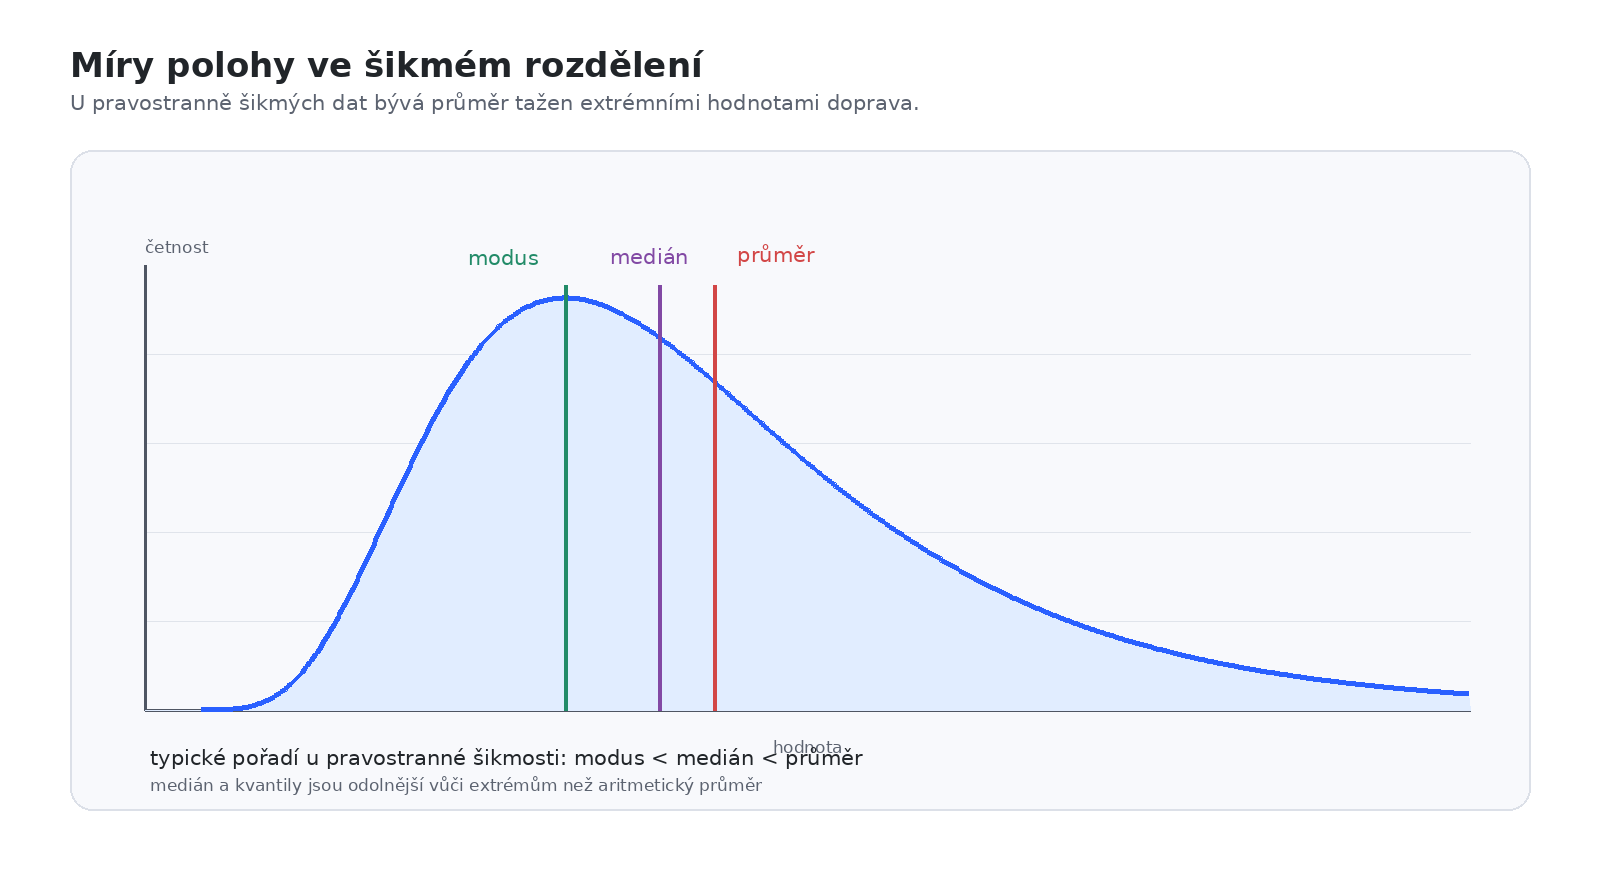
\includegraphics[width=0.95\linewidth]{assets/images/deskriptivni-statistika/mean-median-skewness.png}
  \caption[Míry polohy ve šikmém rozdělení]{Průměr, medián a modus ve šikmém rozdělení. Popis obrázku:
  pravostranně šikmá křivka ukazuje, že průměr je tažen delším pravým ocasem, zatímco medián a modus
  zůstávají blíže hlavní koncentraci hodnot. Zdroj obrázku: vlastní schéma podle obecných vlastností
  měr polohy.}
  \label{fig:mean-median-skewness}
\end{figure}

\subsection*{Míry variability}
\term{Variabilita} popisuje, jak moc se hodnoty liší. Dvě skupiny mohou mít stejný průměr, ale úplně
jinou stabilitu. Pro řízení firmy je často rozdíl mezi průměrem a variabilitou zásadní: stabilní
proces s menším rozptylem může být hodnotnější než proces se stejným průměrem, ale velkými výkyvy.

\term{Rozpětí}:
\[
  R = x_{\max} - x_{\min}.
\]
Je jednoduché, ale závisí jen na dvou extrémních hodnotách.

\term{Rozptyl} a \term{směrodatná odchylka}:
\[
  s^2 = \frac{1}{n-1}\sum_{i=1}^{n}(x_i-\bar{x})^2,
  \qquad
  s = \sqrt{s^2}.
\]
Rozptyl měří průměrnou čtvercovou odchylku od průměru. Směrodatná odchylka vrací měřítko do původních
jednotek. Obě míry jsou citlivé na extrémy, protože odchylky jsou umocněné.

\term{Interkvartilové rozpětí}:
\[
  IQR = Q_3 - Q_1.
\]
Popisuje šířku prostředních 50\% hodnot. Je robustnější vůči extrémům než rozpětí a směrodatná odchylka.

\term{Variační koeficient}:
\[
  CV = \frac{s}{\bar{x}}.
\]
Vyjadřuje relativní variabilitu vůči průměru. Hodí se pro porovnání variability ukazatelů v různých
jednotkách nebo s různou úrovní, například tržeb dvou produktů. Smysl má hlavně pro kladná poměrová
data a nenulový průměr.

\subsection*{Boxplot a odlehlé hodnoty}
\term{Boxplot} neboli krabicový graf shrnuje rozdělení pomocí mediánu, kvartilů, IQR, vousů a
potenciálních odlehlých hodnot. Je vhodný hlavně pro porovnání kvantitativní proměnné mezi skupinami,
například hodnoty objednávky podle kanálu nebo mzdy podle regionu.

Tukeyho pravidlo pro označení potenciálních odlehlých hodnot:
\[
  x < Q_1 - 1{,}5IQR
  \quad \text{nebo} \quad
  x > Q_3 + 1{,}5IQR.
\]
Přísnější hranice používá \(3IQR\). Tyto hranice neznamenají, že se má hodnota automaticky smazat.
Outlier může být chyba, ale také důležitý obchodní případ, podvod, výpadek, VIP zákazník nebo změna
procesu.

\begin{figure}[htbp]
  \centering
  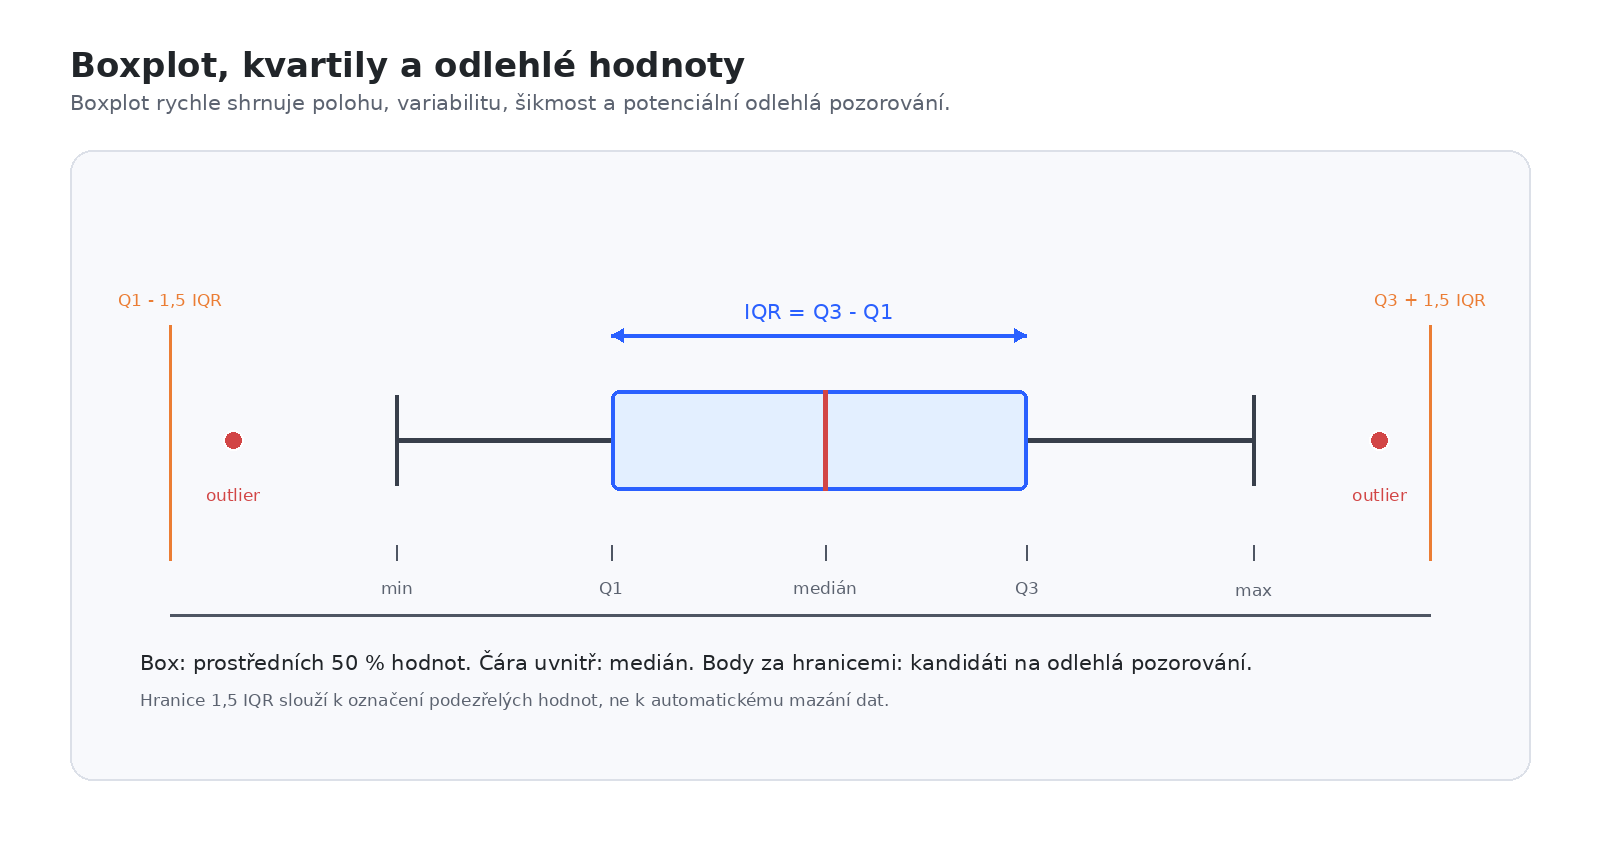
\includegraphics[width=0.95\linewidth]{assets/images/deskriptivni-statistika/boxplot-iqr-outliers.png}
  \caption[Boxplot a IQR]{Boxplot, kvartily a potenciální odlehlé hodnoty. Popis obrázku: krabice
  reprezentuje prostředních 50\% hodnot, čára uvnitř medián, vousy běžný rozsah a body za hranicemi
  1,5 IQR kandidáty na odlehlá pozorování. Zdroj obrázku: vlastní schéma podle Tukeyho boxplotu.}
  \label{fig:boxplot-iqr-outliers}
\end{figure}

\subsection*{Tvar rozdělení}
Kromě polohy a variability se sleduje \term{tvar rozdělení}. Ten je důležitý pro interpretaci statistik
i pro výběr dalších metod.

\term{Šikmost} popisuje asymetrii rozdělení. Pravostranně šikmé rozdělení má dlouhý pravý ocas,
typicky u příjmů, tržeb zákazníků nebo čekacích dob. Levostranně šikmé rozdělení má dlouhý levý ocas.
U pravostranné šikmosti často platí průměr \(>\) medián.

\term{Špičatost} nebo \term{kurtóza} popisuje těžkost ocasů vůči referenčnímu rozdělení. V praxi je
důležité hlavně vědět, zda jsou v datech těžké ocasy a extrémy. Různé softwary používají různé
konvence: někde má normální rozdělení kurtózu 3, jinde se používá nadměrná kurtóza, kde má normální
rozdělení hodnotu 0.

Graficky se tvar rozdělení kontroluje histogramem, boxplotem, hustotou, případně Q-Q grafem. Samotná
tabulka průměru a směrodatné odchylky může podstatnou strukturu skrýt.

\subsection*{Agregace dat}
\term{Agregace} je shrnutí detailních dat na vyšší úroveň. Z transakcí na úrovni položky objednávky
lze například vytvořit denní tržby, měsíční počet zákazníků, tržby podle regionu nebo průměrnou
hodnotu objednávky podle kanálu.

Při agregaci se rozlišují:
\begin{itemize}
  \item \term{dimenze} - hledisko členění, například čas, region, produkt, zákazník nebo kanál;
  \item \term{metrika} - měřená veličina, například tržby, náklady, marže, počet objednávek;
  \item \term{granularita} - úroveň detailu, například den versus měsíc, objednávka versus položka;
  \item \term{agregační funkce} - součet, počet, průměr, medián, minimum, maximum, podíl nebo unikátní
  počet.
\end{itemize}

Zásadní je rozlišovat \term{aditivní}, \term{semiaditivní} a \term{neaditivní} metriky. Tržby lze
sčítat přes produkty i čas. Stav účtu lze sčítat přes zákazníky, ale ne přes dny, protože by vznikl
nesmyslný součet stavů. Poměry, například marže v procentech nebo konverzní poměr, se obvykle nemají
průměrovat bez vah; správně se často počítají z agregovaných čitatelů a jmenovatelů.

Příklad špatné a správné agregace:
\begin{itemize}
  \item špatně: průměrná konverze z průměrů jednotlivých kampaní bez ohledu na návštěvnost;
  \item správně: celková konverze \(= \text{počet konverzí} / \text{počet návštěv}\).
\end{itemize}

\subsection*{Odvozené ukazatele a KPI}
\term{Odvozený ukazatel} vzniká výpočtem z jiných proměnných. V ekonomických datech jde například o:
\begin{itemize}
  \item marži \(= \text{tržby} - \text{náklady}\);
  \item maržovost \(= \text{marže} / \text{tržby}\);
  \item průměrnou hodnotu objednávky \(= \text{tržby} / \text{počet objednávek}\);
  \item konverzní poměr \(= \text{počet konverzí} / \text{počet návštěv}\);
  \item jednotkové náklady \(= \text{náklady} / \text{počet jednotek}\);
  \item meziroční růst \(= x_t/x_{t-12}-1\), pokud pracujeme s měsíčními daty.
\end{itemize}

\term{KPI} je klíčový ukazatel výkonnosti. KPI má být navázaný na cíl, mít jasnou definici, vlastníka,
periodicitu, zdroj dat a interpretační pravidla. Nestačí zobrazit mnoho metrik. Užitečné KPI odpovídá
na otázku, zda se organizace přibližuje ke konkrétnímu cíli.

\subsection*{Komparace ekonomických dat}
\term{Komparace} znamená porovnávání hodnot mezi obdobími, skupinami, plánem a skutečností nebo vůči
benchmarku. Ekonomická data se často porovnávají relativně, protože absolutní rozdíl bez kontextu
může být zavádějící.

Základní porovnání:
\[
  \Delta x = x_t - x_0,
  \qquad
  r = \frac{x_t}{x_0} - 1.
\]
\(\Delta x\) je absolutní změna, \(r\) relativní změna. V procentech se relativní změna násobí 100.

\term{Bazický index} porovnává všechna období se stejným základním obdobím:
\[
  I_t^b = 100 \cdot \frac{x_t}{x_b}.
\]
Hodnota 125 znamená, že ukazatel je o 25\% vyšší než v bázi.

\term{Řetězový index} porovnává období s předchozím obdobím:
\[
  I_t^r = 100 \cdot \frac{x_t}{x_{t-1}}.
\]
Hodí se pro sledování dynamiky krok za krokem. Řetězové tempo růstu je \(I_t^r - 100\) procentních
bodů, případně \(x_t/x_{t-1}-1\) v desetinném zápisu.

\begin{figure}[htbp]
  \centering
  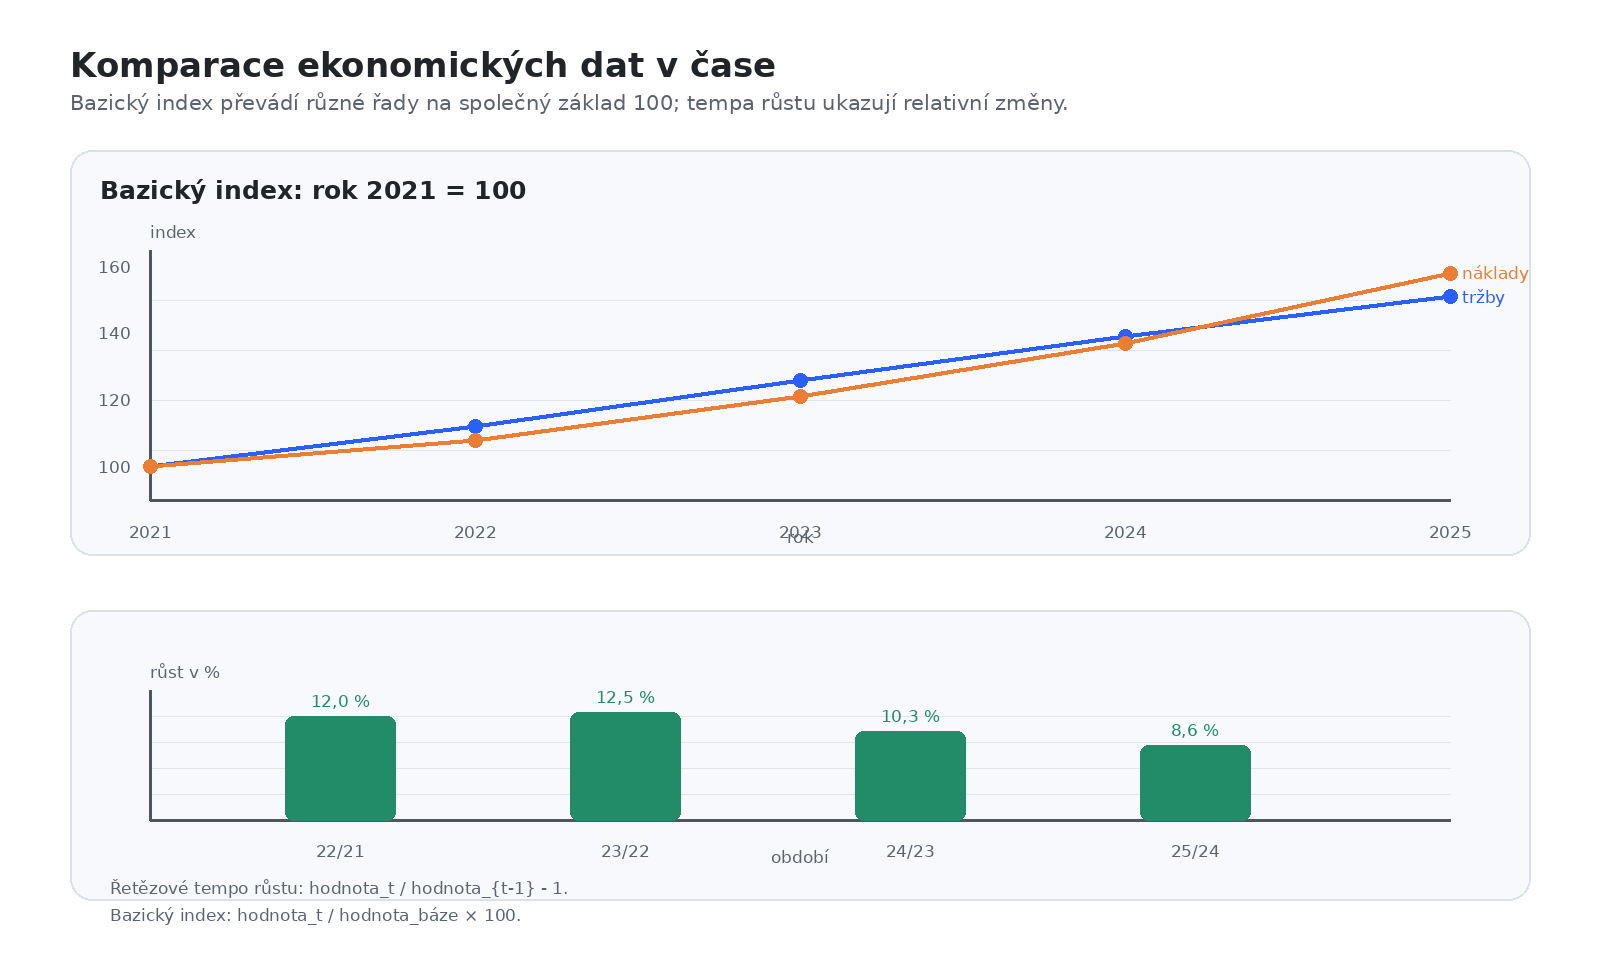
\includegraphics[width=0.95\linewidth]{assets/images/deskriptivni-statistika/economic-comparison-indices.png}
  \caption[Bazický index a tempa růstu]{Komparace ekonomických dat pomocí bazického indexu a řetězových
  temp růstu. Popis obrázku: horní panel převádí tržby a náklady na společný základ 2021 = 100, dolní
  panel ukazuje řetězová tempa růstu mezi sousedními obdobími. Zdroj obrázku: vlastní schéma.}
  \label{fig:economic-comparison-indices}
\end{figure}

U ekonomické komparace je potřeba hlídat:
\begin{itemize}
  \item zda jde o nominální nebo reálné hodnoty očištěné o cenovou změnu;
  \item zda jsou období stejně dlouhá a srovnatelná;
  \item zda sezonnost nezkresluje meziměsíční porovnání;
  \item zda se nezměnila definice ukazatele, datový zdroj nebo metodika;
  \item zda se procentní body nezaměňují s procenty.
\end{itemize}

Příklad rozdílu mezi procenty a procentními body: pokud podíl vzrostl z 10\% na 12\%, zvýšil se o
2 procentní body, ale relativně o 20\%.

U souhrnných cenových a objemových indexů je dobré znát rozdíl mezi \term{Laspeyresovým} indexem
s vahami ze základního období, \term{Paascheho} indexem s vahami běžného období a \term{Fisherovým}
indexem jako jejich geometrickým průměrem. V praxi se tím řeší, zda změnu cen měříme při staré nebo
aktuální struktuře spotřeby či produkce.

V reportingu se často používá i časová komparace typu \term{YTD} -- kumulace od začátku roku do
aktuálního období -- a \term{YoY}, tedy meziroční srovnání stejného období. U sezonných dat je YoY
často smysluplnější než prosté porovnání s bezprostředně předchozím měsícem.

\subsection*{Kontingenční analýza a vztahy mezi proměnnými}
Deskriptivní analýza nemusí popisovat jen jednu proměnnou. Často sleduje vztah dvou proměnných.

\term{Kontingenční tabulka} zobrazuje četnosti kombinací dvou kategoriálních proměnných, například
regionu a typu zákazníka. Z ní lze počítat řádková procenta, sloupcová procenta a celkové podíly.
Řádková procenta odpovídají na otázku \uv{jaká je struktura uvnitř řádku}, sloupcová procenta na
otázku \uv{jak se skládá daný sloupec}.

U dvou kvantitativních proměnných se často používá \term{korelace}. Pearsonův korelační koeficient
popisuje lineární vztah, Spearmanova korelace vztah pořadí. Korelace je deskriptivní míra asociace,
ne důkaz kauzality.

U kombinace kvantitativní a kategoriální proměnné se porovnávají skupinové statistiky: průměr, medián,
IQR, směrodatná odchylka a počet pozorování v každé skupině. Graficky se hodí boxplot nebo sloupcový
graf s intervaly nejistoty, pokud chceme ukázat i spolehlivost odhadu.

\subsection*{Základy statistické inference a testování hypotéz}
Deskriptivní statistika popisuje pozorovaná data. Často ale chceme udělat krok dál: z výběru usuzovat
na širší populaci nebo rozhodnout, zda pozorovaný rozdíl může být jen náhodná výběrová chyba. K tomu
slouží \term{statistická inference}.

Základní rozlišení:
\begin{itemize}
  \item \term{populace} je celek, o kterém chceme něco říct, například všichni zákazníci firmy;
  \item \term{výběr} je pozorovaná část populace, například zákazníci v konkrétním dotazníku;
  \item \term{parametr} je neznámá vlastnost populace, například skutečný průměr \(\mu\);
  \item \term{statistika} je hodnota spočítaná z výběru, například výběrový průměr \(\bar{x}\).
\end{itemize}

Výběrová statistika je zatížená nejistotou. Proto se kromě bodového odhadu často uvádí
\term{standardní chyba}:
\[
  SE(\bar{x})=\frac{s}{\sqrt{n}}.
\]
Čím větší je výběr a čím menší je variabilita dat, tím menší je standardní chyba.

\subsubsection*{Interval spolehlivosti}
Interval spolehlivosti ukazuje rozumný rozsah hodnot populačního parametru. Pro průměr se často zapisuje:
\[
  \bar{x}\pm t_{1-\alpha/2,n-1}\frac{s}{\sqrt{n}}.
\]
U 95\% intervalu volíme \(\alpha=0{,}05\). Širší interval znamená větší nejistotu. Důležité je neříkat,
že \uv{parametr má 95\% pravděpodobnost ležet v tomto konkrétním intervalu}. Ve frekvenční interpretaci
by při opakovaném stejném postupu dlouhodobě přibližně 95\% takto vytvořených intervalů obsahovalo
skutečný parametr.

\subsubsection*{Postup testování hypotéz}
Testování hypotéz převádí věcnou otázku na statistické rozhodnutí.

Typický postup:
\begin{enumerate}
  \item formulovat nulovou hypotézu \(H_0\), obvykle \uv{žádný rozdíl} nebo \uv{žádný efekt};
  \item formulovat alternativu \(H_1\), například oboustrannou \( \mu \neq \mu_0 \) nebo jednostrannou
  \( \mu > \mu_0 \);
  \item zvolit hladinu významnosti \(\alpha\), často 0{,}05;
  \item spočítat testovou statistiku;
  \item určit \(p\)-value nebo porovnat testovou statistiku s kritickou hodnotou;
  \item rozhodnout, zda \(H_0\) zamítáme, a hlavně výsledek věcně interpretovat.
\end{enumerate}

\term{\(p\)-value} je pravděpodobnost, že bychom při platnosti nulové hypotézy pozorovali stejně
extrémní nebo extrémnější testovou statistiku, než jakou jsme dostali v datech. Pokud:
\[
  p\text{-value}<\alpha,
\]
zamítáme \(H_0\) na hladině významnosti \(\alpha\).

Pozor: \(p\)-value není pravděpodobnost, že je nulová hypotéza pravdivá. Také neříká, jak velký nebo
prakticky důležitý je efekt. Malé \(p\)-value může vzniknout u velmi malého, ale přesně odhadnutého
rozdílu ve velkém vzorku.

\subsubsection*{Chyby prvního a druhého druhu}
Při testování můžeme udělat dva základní typy chyb:
\begin{itemize}
  \item \term{chyba I. druhu} - zamítneme pravdivou \(H_0\); její pravděpodobnost kontroluje
  \(\alpha\);
  \item \term{chyba II. druhu} - nezamítneme \(H_0\), i když je ve skutečnosti nepravdivá;
  \item \term{síla testu} je pravděpodobnost správně zamítnout nepravdivou \(H_0\).
\end{itemize}

Snížení \(\alpha\) zmenšuje riziko falešně pozitivního závěru, ale při stejném rozsahu dat obvykle
zvyšuje riziko, že skutečný efekt neodhalíme.

\subsubsection*{t-test}
\term{t-test} se používá hlavně pro testování průměrů, když neznáme populační rozptyl a pracujeme s
výběrovou směrodatnou odchylkou.

Jednovýběrový t-test:
\[
  H_0:\mu=\mu_0,
  \qquad
  t=\frac{\bar{x}-\mu_0}{s/\sqrt{n}}.
\]

Dvouvýběrový t-test porovnává průměry dvou nezávislých skupin:
\[
  H_0:\mu_1-\mu_2=0.
\]
V praxi se často používá Welchův t-test, protože nevyžaduje stejný rozptyl ve skupinách:
\[
  t=
  \frac{\bar{x}_1-\bar{x}_2}
  {\sqrt{s_1^2/n_1+s_2^2/n_2}}.
\]

Párový t-test se používá, když máme dvojice pozorování, například stejný zákazník před a po změně
ceny. Potom testujeme průměr rozdílů:
\[
  d_i=x_{i,\text{po}}-x_{i,\text{před}},
  \qquad
  H_0:\mu_d=0.
\]

Před t-testem je potřeba vědět, co přesně jsou skupiny, zda jsou pozorování nezávislá, zda nejde o
párová data a zda extrémy nebo silná šikmost nedělají průměr zavádějícím.

\subsubsection*{F-test}
\term{F-test} používá testovou statistiku s F-rozdělením. Typicky vzniká jako poměr dvou odhadů
rozptylu nebo jako porovnání vysvětlené a nevysvětlené variability.

Test shody dvou rozptylů:
\[
  H_0:\sigma_1^2=\sigma_2^2,
  \qquad
  F=\frac{s_1^2}{s_2^2}.
\]
Tento test je citlivý na odchylky od normality. Pokud jsou data šikmá nebo mají těžké ocasy, bývá
vhodnější robustnější test rovnosti rozptylů, například Leveneho test.

V analýze rozptylu (ANOVA) se F-test používá k porovnání více skupinových průměrů:
\[
  H_0:\mu_1=\mu_2=\cdots=\mu_g.
\]
Princip je porovnat variabilitu mezi skupinami s variabilitou uvnitř skupin:
\[
  F=\frac{\text{variabilita mezi skupinami}}{\text{variabilita uvnitř skupin}}.
\]
Velké \(F\) znamená, že rozdíly mezi skupinovými průměry jsou velké vzhledem k běžné variabilitě uvnitř
skupin.

V regresi se F-test používá také pro společnou významnost více koeficientů, například zda několik
vysvětlujících proměnných jako celek zlepšuje model. Zkouškově je důležité vědět, že t-test se často
ptá na jeden parametr, zatímco F-test se často ptá na více omezení najednou.

\subsection*{Chybějící hodnoty a kvalita dat}
Deskriptivní analýza má začít kontrolou kvality dat. Bez ní mohou být všechny statistiky formálně
správné, ale věcně zavádějící.

Kontroluje se hlavně:
\begin{itemize}
  \item počet řádků a unikátních identifikátorů;
  \item duplicity;
  \item chybějící hodnoty podle proměnných a skupin;
  \item neplatné kategorie a hodnoty mimo povolený rozsah;
  \item extrémní hodnoty;
  \item jednotky, měny, časová pásma a formáty;
  \item konzistence mezi souvisejícími poli, například datum objednávky před datem doručení.
\end{itemize}

Chybějící hodnoty nelze řešit mechanicky. Je rozdíl mezi \uv{neznámé}, \uv{nevztahuje se},
\uv{odmítnuto odpovědět} a \uv{chyba importu}. Před imputací nebo odstraněním je potřeba zjistit,
zda chybění není systematické, například častější u určitého regionu nebo segmentu.

\subsection*{Praktický postup deskriptivní analýzy}
Typický postup:
\begin{enumerate}
  \item vymezit analytickou otázku, jednotku pozorování a cílové publikum;
  \item zkontrolovat strukturu dat, typy proměnných, jednotky a chybějící hodnoty;
  \item spočítat základní četnosti a souhrnné statistiky;
  \item zobrazit rozdělení klíčových proměnných histogramem, boxplotem nebo hustotou;
  \item porovnat hodnoty podle hlavních dimenzí;
  \item ověřit agregace, váhy a definice odvozených metrik;
  \item interpretovat výsledky věcně, ne jen mechanicky podle čísel;
  \item zdokumentovat zdroj, období, filtry, definice a omezení.
\end{enumerate}

\subsection*{Nástroje}
Deskriptivní statistiku lze dělat v tabulkových procesorech, databázích, programovacích jazycích
i BI nástrojích.

\begin{center}
\small
\begin{tabular}{@{}>{\raggedright\arraybackslash}p{0.24\textwidth}
                >{\raggedright\arraybackslash}p{0.30\textwidth}
                >{\raggedright\arraybackslash}p{0.35\textwidth}@{}}
\hline
\term{Nástroj} & \term{Příklady funkcí} & \term{Typické použití} \\
\hline
Excel / Google Sheets & kontingenční tabulky, \texttt{AVERAGE}, \texttt{MEDIAN}, grafy & rychlé
ad hoc přehledy a menší datové sady \\
SQL & \texttt{GROUP BY}, \texttt{COUNT}, \texttt{SUM}, \texttt{AVG}, \texttt{MIN}, \texttt{MAX} &
agregace přímo v databázi \\
Python & pandas \texttt{describe}, \texttt{groupby}, \texttt{pivot\_table}; seaborn, matplotlib &
opakovatelná analýza, větší datové sady, notebooky \\
R & \texttt{summary}, \texttt{aggregate}, \texttt{dplyr}, \texttt{ggplot2} & statistická analýza
a publikovatelné grafy \\
BI nástroje & Power BI, Tableau, Qlik & dashboardy, KPI, drill-down, sdílené reporty \\
\hline
\end{tabular}
\end{center}

\pozor
Nejčastější chyba u zkoušky je vyjmenovat průměr, medián a směrodatnou odchylku bez kontextu. Správná
odpověď musí říct, kdy která statistika dává smysl, jak ji ovlivňují extrémy, jak se agregují metriky
a jak se porovnávají ekonomická data. Druhá častá chyba je průměrovat poměry bez vah nebo zaměnit
procenta a procentní body.

U testování hypotéz je nejčastější chyba říct, že \(p\)-value je pravděpodobnost platnosti nulové
hypotézy. Není. Je to pravděpodobnost tak extrémní testové statistiky za předpokladu, že \(H_0\) platí.
Statistická významnost také není totéž co věcná významnost. U velkých dat může být i malý a prakticky
nevýznamný rozdíl statisticky významný.

\subsection*{Shrnutí ke zkoušce}
\begin{itemize}
  \item Deskriptivní analýza popisuje již pozorovaná data; neprokazuje kauzalitu a sama o sobě
  nepredikuje budoucnost.
  \item Volba statistiky závisí na typu proměnné: nominální, ordinální, intervalové nebo poměrové.
  \item Četnostní analýza pracuje s absolutními, relativními a kumulativními četnostmi.
  \item Míry polohy zahrnují průměr, vážený průměr, medián, modus a kvantily.
  \item Míry variability zahrnují rozpětí, rozptyl, směrodatnou odchylku, IQR a variační koeficient.
  \item Medián, IQR a MAD jsou robustnější vůči extrémům než průměr a směrodatná odchylka.
  \item Histogram a boxplot pomáhají odhalit šikmost, těžké ocasy, vícemodalitu a odlehlé hodnoty.
  \item Agregace vyžaduje správnou granularitu, dimenze, metriky a agregační funkce.
  \item Poměrové ukazatele je často nutné počítat z agregovaných čitatelů a jmenovatelů, ne jako
  prostý průměr procent.
  \item Ekonomická data se porovnávají absolutní změnou, relativní změnou, bazickými a řetězovými
  indexy, tempy růstu a benchmarky.
  \item U interpretace je nutné hlídat kvalitu dat, chybějící hodnoty, změny metodiky, sezonnost,
  inflaci a srovnatelnost období.
  \item Základní inferenční postup rozlišuje populaci, výběr, parametr, statistiku, standardní chybu,
  interval spolehlivosti a test hypotézy.
  \item \(p\)-value porovnává pozorovaný výsledek s tím, co by bylo očekávatelné při platnosti nulové
  hypotézy; malé \(p\)-value samo o sobě neříká, že efekt je velký nebo kauzální.
  \item t-test se používá hlavně pro testování průměrů; F-test pro poměry rozptylů, ANOVA a společné
  testování více omezení.
\end{itemize}

\subsection*{Zdroje}
\begin{itemize}
  \item NIST/SEMATECH e-Handbook of Statistical Methods: \href{https://itl.nist.gov/div898/handbook/eda/eda.htm}{Exploratory Data Analysis}.
  \item NIST/SEMATECH e-Handbook of Statistical Methods: \href{https://www.itl.nist.gov/div898/handbook/eda/section3/eda351.htm}{Measures of Location}.
  \item NIST/SEMATECH e-Handbook of Statistical Methods: \href{https://www.itl.nist.gov/div898/handbook/eda/section3/eda356.htm}{Measures of Scale}.
  \item NIST/SEMATECH e-Handbook of Statistical Methods: \href{https://www.itl.nist.gov/div898/handbook/eda/section3/histogra.htm}{Histogram}.
  \item NIST/SEMATECH e-Handbook of Statistical Methods: \href{https://www.itl.nist.gov/div898/handbook/eda/section3/boxplot.htm}{Box Plot}.
  \item NIST/SEMATECH e-Handbook of Statistical Methods: \href{https://www.itl.nist.gov/div898/handbook/eda/section3/eda35b.htm}{Measures of Skewness and Kurtosis}.
  \item NIST/SEMATECH e-Handbook of Statistical Methods: \href{https://www.itl.nist.gov/div898/handbook/prc/section1/prc131.htm}{Critical values and p values}.
  \item NIST/SEMATECH e-Handbook of Statistical Methods: \href{https://itl.nist.gov/div898/handbook/eda/section3/eda359.htm}{F-Test for Equality of Two Variances}.
  \item NIST Dataplot Reference Manual: \href{https://www.itl.nist.gov/div898/software/dataplot/refman1/auxillar/t\_test.htm}{T TEST}.
  \item PennState STAT 500: \href{https://online.stat.psu.edu/stat500/Lesson06.html}{Hypothesis Testing}.
  \item R Documentation: \href{https://stat.ethz.ch/R-manual/R-devel/library/stats/html/IQR.html}{The Interquartile Range}.
  \item OECD: \href{https://www.oecd.org/en/publications/oecd-glossary-of-statistical-terms_9789264055087-en.html}{OECD Glossary of Statistical Terms}.
\end{itemize}

\newpage

\section{Exploratorní analýza. Redukce rozměru dat, hlavní komponenty, faktorová, korespondenční a diskriminační analýza}

\subsection*{Základní myšlenka exploratorní analýzy}

Exploratorní analýza dat, zkráceně EDA, slouží k tomu, abychom data nejdříve pochopili, než na ně
začneme aplikovat formální modely. Cílem není hned dokazovat hypotézy, ale:
\begin{itemize}
    \item zobrazit a shrnout data,
    \item najít zajímavé vzory a struktury,
    \item odhalit odlehlá pozorování a chyby,
    \item ověřit vhodnost proměnných pro další analýzu,
    \item zjednodušit data, pokud mají mnoho proměnných nebo pozorování.
\end{itemize}

EDA typicky používá:
\begin{itemize}
    \item deskriptivní statistiky,
    \item grafy,
    \item korelační analýzu,
    \item redukci dimenze,
    \item shlukování,
    \item metody pro detekci odlehlých hodnot.
\end{itemize}

\subsection*{Příprava dat před redukčními metodami}

Před metodami jako PCA, faktorová analýza, korespondenční analýza nebo diskriminační analýza je potřeba
data zkontrolovat.

\begin{itemize}
    \item \textbf{Deskriptivní statistiky:} průměr, medián, směrodatná odchylka, minimum, maximum,
    kvartily.
    
    \item \textbf{Grafická kontrola:} histogramy, boxploty, scatterploty, korelační grafy.
    
    \item \textbf{Chybějící hodnoty:} mnoho redukčních metod neumí přímo pracovat s missing values.
    Je nutné je odstranit nebo imputovat.
    
    \item \textbf{Odlehlé hodnoty:} outliery mohou výrazně ovlivnit kovarianční/korelační matici,
    a tím i PCA, faktorovou i diskriminační analýzu.
    
    \item \textbf{Normalizace/standardizace:} proměnné v různých měřítkách mohou vést k tomu, že
    proměnná s velkou variabilitou dominuje výsledku.
\end{itemize}

Standardizace proměnné:
\[
z_{ij}
=
\frac{x_{ij}-\bar{x}_j}{s_j}.
\]

Používá se hlavně tehdy, když jsou proměnné v různých jednotkách, například příjem v Kč,
věk v letech a počet nákupů v kusech.

\subsection*{Odlehlé hodnoty v EDA}

Odlehlé pozorování je hodnota, která se výrazně liší od většiny dat. Může jít o chybu měření,
chybu zápisu, ale také o skutečně extrémní a informativní pozorování.

\subsubsection*{Z-score metoda}

\[
z_i = \frac{x_i-\bar{x}}{s}.
\]

Za potenciální outlier se často považuje pozorování:
\[
|z_i|>3.
\]

Tato metoda je jednoduchá, ale předpokládá přibližně normální rozdělení a není robustní vůči extrémům.

\subsubsection*{IQR metoda a Tukeyho hranice}

Interkvartilové rozpětí:
\[
IQR = Q_3-Q_1.
\]

Mírné outliery:
\[
x_i < Q_1 - 1.5IQR
\quad \text{nebo} \quad
x_i > Q_3 + 1.5IQR.
\]

Extrémní outliery:
\[
x_i < Q_1 - 3IQR
\quad \text{nebo} \quad
x_i > Q_3 + 3IQR.
\]

Výhodou je větší robustnost než u z-score metody.

\subsubsection*{Mahalanobisova vzdálenost}

Pro vícerozměrná data:
\[
D_i^2
=
(\mathbf{x}_i-\bar{\mathbf{x}})^\top
S^{-1}
(\mathbf{x}_i-\bar{\mathbf{x}}),
\]
kde $S$ je kovarianční matice.

Mahalanobisova vzdálenost bere v úvahu:
\begin{itemize}
    \item vzdálenost od vícerozměrného průměru,
    \item variabilitu proměnných,
    \item korelace mezi proměnnými.
\end{itemize}

Je proto vhodnější pro vícerozměrné outliery než posuzování každé proměnné zvlášť.

\subsection*{Redukce rozměru dat}

Redukční metody se používají, když je dataset příliš složitý:
\begin{itemize}
    \item má mnoho proměnných,
    \item proměnné spolu silně korelují,
    \item data se obtížně vizualizují,
    \item chceme odstranit redundanci,
    \item chceme získat menší počet nových, lépe interpretovatelných dimenzí.
\end{itemize}

Rozlišujeme:
\begin{itemize}
    \item \textbf{redukci počtu proměnných} -- PCA, faktorová analýza,
    \item \textbf{redukci počtu pozorování} -- shluková analýza,
    \item \textbf{redukci kategoriálních vztahů} -- korespondenční analýza,
    \item \textbf{redukci s ohledem na známé skupiny} -- diskriminační analýza.
\end{itemize}

\subsection*{Analýza hlavních komponent}

Analýza hlavních komponent, PCA, je metoda pro redukci počtu kvantitativních proměnných.
Původní proměnné nahradí menším počtem nových proměnných, které se nazývají hlavní komponenty.

\subsubsection*{Základní idea PCA}

PCA hledá lineární kombinace původních proměnných:
\[
z_1 = a_{11}x_1+a_{12}x_2+\cdots+a_{1p}x_p,
\]
\[
z_2 = a_{21}x_1+a_{22}x_2+\cdots+a_{2p}x_p,
\]
atd.

Tyto nové proměnné mají dvě důležité vlastnosti:
\begin{itemize}
    \item jsou navzájem nekorelované,
    \item první komponenta vysvětluje co největší část variability dat,
    druhá komponenta co největší část zbývající variability atd.
\end{itemize}

\subsubsection*{Maticový zápis PCA}

Mějme datovou matici:
\[
X \in \mathbb{R}^{n \times p},
\]
kde $n$ je počet pozorování a $p$ počet proměnných.

Předpokládejme, že proměnné jsou centrované, případně standardizované.

Kovarianční matice:
\[
S = \frac{1}{n-1}X^\top X.
\]

Pokud pracujeme se standardizovanými proměnnými, pak $S$ odpovídá korelační matici.

PCA je založená na vlastních číslech a vlastních vektorech:
\[
S\mathbf{v}_j = \lambda_j \mathbf{v}_j.
\]

Kde:
\begin{itemize}
    \item $\lambda_j$ je vlastní číslo,
    \item $\mathbf{v}_j$ je vlastní vektor,
    \item vlastní vektor určuje směr komponenty,
    \item vlastní číslo říká, kolik variability daná komponenta vysvětluje.
\end{itemize}

První hlavní komponenta odpovídá největšímu vlastnímu číslu:
\[
\lambda_1 \geq \lambda_2 \geq \cdots \geq \lambda_p.
\]

Skóre hlavních komponent:
\[
Z = XV,
\]
kde $V$ je matice vlastních vektorů.

\subsubsection*{Vysvětlená variabilita}

Celková variabilita:
\[
\sum_{j=1}^p \lambda_j.
\]

Podíl variability vysvětlený $j$-tou komponentou:
\[
\frac{\lambda_j}{\sum_{\ell=1}^p \lambda_\ell}.
\]

Kumulativní vysvětlená variabilita prvních $m$ komponent:
\[
\frac{\sum_{j=1}^m \lambda_j}
{\sum_{\ell=1}^p \lambda_\ell}.
\]

\subsubsection*{Volba počtu komponent}

Počet komponent lze volit podle:
\begin{itemize}
    \item \textbf{kumulativní vysvětlené variability} -- např. vybereme tolik komponent,
    aby vysvětlily 70--90~\% variability,
    
    \item \textbf{scree plotu} -- hledáme bod zlomu, po kterém další komponenty přidávají
    už jen málo informace,
    
    \item \textbf{Kaiserova kritéria} -- u PCA z korelační matice ponecháme komponenty s
    \[
    \lambda_j>1,
    \]
    
    \item \textbf{interpretovatelnosti} -- komponenty musí dávat věcný smysl.
\end{itemize}

\subsubsection*{Interpretace komponent}

Komponenty interpretujeme podle vah původních proměnných ve vlastních vektorech.
Pokud má první komponenta velké kladné váhy u proměnných příjem, útrata a hodnota majetku,
můžeme ji interpretovat například jako \uv{ekonomickou sílu}.

Často se používají také \textbf{loadings}, tedy vztahy mezi původními proměnnými a komponentami:
\[
\ell_{jk}
=
\operatorname{cor}(x_j,z_k).
\]

Velké absolutní hodnoty loadings říkají, že daná proměnná silně souvisí s danou komponentou.

\subsubsection*{Rekonstrukce dat}

Pokud ponecháme jen prvních $m<p$ komponent, dostaneme redukovanou aproximaci dat:
\[
\hat X_m = Z_m V_m^\top.
\]

Čím větší je $m$, tím přesnější je rekonstrukce, ale tím menší je redukce.

\subsubsection*{Výhody a nevýhody PCA}

Výhody:
\begin{itemize}
    \item snižuje počet proměnných,
    \item odstraňuje multikolinearitu,
    \item umožňuje vizualizovat vícerozměrná data ve 2D nebo 3D,
    \item zachovává co nejvíce variability.
\end{itemize}

Nevýhody:
\begin{itemize}
    \item komponenty nemusí být snadno interpretovatelné,
    \item PCA je citlivá na škálování proměnných,
    \item PCA je citlivá na outliery,
    \item PCA maximalizuje variabilitu, ne nutně vztah k cílové proměnné.
\end{itemize}

\subsection*{Regrese hlavních komponent}

Regrese hlavních komponent, PCR, kombinuje PCA a lineární regresi.

Nejprve se z původních vysvětlujících proměnných vytvoří hlavní komponenty:
\[
Z = XV.
\]

Potom se odhaduje regresní model:
\[
y = \alpha+\gamma_1 z_1+\cdots+\gamma_m z_m+u.
\]

PCR se používá hlavně při:
\begin{itemize}
    \item silné multikolinearitě vysvětlujících proměnných,
    \item velkém počtu proměnných,
    \item predikčních úlohách.
\end{itemize}

Nevýhoda je, že PCA vybírá komponenty podle variability v $X$, nikoli podle toho, jak dobře vysvětlují $y$.
Komponenta s malou variabilitou může být pro predikci $y$ důležitá, ale PCA ji může odstranit.

\subsection*{Faktorová analýza}

Faktorová analýza se podobá PCA, ale její cíl je jiný. PCA hledá nové proměnné, které vysvětlují
variabilitu dat. Faktorová analýza předpokládá, že za pozorovanými proměnnými stojí menší počet
nepozorovaných latentních faktorů.

\subsubsection*{Základní idea}

Příklad:
\begin{itemize}
    \item otázky v dotazníku o spokojenosti,
    \item ekonomické ukazatele regionů,
    \item psychologické škály,
    \item marketingové proměnné o zákaznících.
\end{itemize}

Mnoho pozorovaných proměnných může být projevem několika latentních faktorů, například:
\begin{itemize}
    \item socioekonomický status,
    \item loajalita zákazníka,
    \item kvalita života,
    \item finanční stabilita.
\end{itemize}

\subsubsection*{Faktorový model}

Standardní faktorový model:
\[
\mathbf{x}
=
\boldsymbol{\mu}
+
\Lambda \mathbf{f}
+
\boldsymbol{\varepsilon}.
\]

Kde:
\begin{itemize}
    \item $\mathbf{x}$ je vektor pozorovaných proměnných,
    \item $\boldsymbol{\mu}$ je vektor středních hodnot,
    \item $\mathbf{f}$ je vektor latentních faktorů,
    \item $\Lambda$ je matice faktorových zátěží,
    \item $\boldsymbol{\varepsilon}$ jsou specifické chyby.
\end{itemize}

Typicky předpokládáme:
\[
\mathrm{E}(\mathbf{f})=0,
\qquad
\mathrm{Var}(\mathbf{f})=I,
\qquad
\mathrm{E}(\boldsymbol{\varepsilon})=0,
\qquad
\mathrm{Cov}(\mathbf{f},\boldsymbol{\varepsilon})=0.
\]

Kovarianční matice pozorovaných proměnných:
\[
\Sigma
=
\Lambda\Lambda^\top+\Psi,
\]
kde $\Psi$ je diagonální matice unikátních rozptylů.

\subsubsection*{Faktorové zátěže}

Prvek $\lambda_{jk}$ v matici $\Lambda$ říká, jak silně je proměnná $x_j$ spojena s faktorem $f_k$.

Vysoká absolutní hodnota:
\[
|\lambda_{jk}|
\]
znamená, že proměnná silně souvisí s daným faktorem.

\subsubsection*{Komunalita a unikátnost}

Komunalita proměnné $x_j$:
\[
h_j^2
=
\sum_{k=1}^m \lambda_{jk}^2.
\]

Komunalita říká, jak velká část variability proměnné je vysvětlena společnými faktory.

Unikátnost:
\[
\psi_j = 1-h_j^2
\]
u standardizovaných proměnných.

Unikátnost vyjadřuje část variability, kterou společné faktory nevysvětlují.

\subsubsection*{Postup faktorové analýzy}

\begin{enumerate}
    \item \textbf{Příprava dat:}
    kontrola missing values, outlierů, škálování a korelací mezi proměnnými.
    
    \item \textbf{Posouzení vhodnosti dat:}
    proměnné by spolu měly dostatečně korelovat. Často se používá KMO kritérium a Bartlettův test
    sphericity.
    
    \item \textbf{Volba počtu faktorů:}
    scree plot, vlastní čísla, teorie, interpretovatelnost.
    
    \item \textbf{Extrakce faktorů:}
    například principal axis factoring nebo maximum likelihood.
    
    \item \textbf{Rotace faktorů:}
    rotace zjednodušuje interpretaci faktorové struktury.
    
    \item \textbf{Interpretace faktorů:}
    faktory pojmenujeme podle proměnných s nejvyššími zátěžemi.
\end{enumerate}

\subsubsection*{Rotace faktorů}

Rotace nemění základní kvalitu vysvětlení, ale snaží se dosáhnout jednodušší interpretace.

\paragraph{Ortogonální rotace.}
Faktory zůstávají nekorelované.
\begin{itemize}
    \item \textbf{Varimax} -- snaží se snížit křížové zátěže a zpřehlednit faktorový model.
    \item \textbf{Quartimax} -- snaží se snížit počet faktorů potřebných k vysvětlení proměnné.
    \item \textbf{Equamax} -- kompromis mezi varimax a quartimax.
\end{itemize}

\paragraph{Šikmá rotace.}
Faktory mohou být korelované.
\begin{itemize}
    \item \textbf{Promax} -- vhodná a efektivní i pro větší datasety.
    \item \textbf{Direct oblimin} -- může vést k jednodušší faktorové struktuře.
\end{itemize}

\subsubsection*{PCA vs. faktorová analýza}

\begin{itemize}
    \item \textbf{PCA} vytváří komponenty jako lineární kombinace pozorovaných proměnných.
    \item \textbf{Faktorová analýza} předpokládá latentní faktory, které způsobují korelace mezi
    pozorovanými proměnnými.
    \item PCA se zaměřuje na vysvětlení celkové variability.
    \item Faktorová analýza se zaměřuje na vysvětlení společné variability.
    \item PCA nemá explicitní chybový člen pro každou proměnnou.
    \item Faktorová analýza rozlišuje společnou a unikátní část variability.
\end{itemize}

\subsection*{Korespondenční analýza}

Korespondenční analýza je metoda pro exploraci vztahů v kontingenční tabulce. Používá se hlavně
pro kategoriální data.

\subsubsection*{Vstupní data}

Máme kontingenční tabulku:
\[
N = (n_{ij}),
\]
kde $n_{ij}$ je četnost v řádku $i$ a sloupci $j$.

Celkový počet pozorování:
\[
n = \sum_i \sum_j n_{ij}.
\]

Matice relativních četností:
\[
P = \frac{1}{n}N.
\]

Řádkové marginální četnosti:
\[
r_i = \sum_j p_{ij}.
\]

Sloupcové marginální četnosti:
\[
c_j = \sum_i p_{ij}.
\]

\subsubsection*{Princip}

Korespondenční analýza zkoumá, jak moc se skutečné četnosti liší od četností očekávaných při nezávislosti
řádkové a sloupcové proměnné.

Očekávaná relativní četnost při nezávislosti:
\[
p_{ij}^{(0)}=r_i c_j.
\]

Odchylka od nezávislosti:
\[
p_{ij}-r_i c_j.
\]

Testová statistika chí-kvadrát:
\[
\chi^2
=
\sum_i\sum_j
\frac{(n_{ij}-nr_ic_j)^2}{nr_ic_j}.
\]

Celková inertia:
\[
I
=
\frac{\chi^2}{n}.
\]

Inertia je analogie vysvětlené variability v PCA. Říká, jak silná je celková asociace mezi řádky a sloupci.

\subsubsection*{Standardizovaná reziduální matice}

Definujeme diagonální matice:
\[
D_r=\operatorname{diag}(r_1,\ldots,r_I),
\qquad
D_c=\operatorname{diag}(c_1,\ldots,c_J).
\]

Standardizovaná reziduální matice:
\[
S
=
D_r^{-1/2}
(P-\mathbf{r}\mathbf{c}^\top)
D_c^{-1/2}.
\]

Na tuto matici se aplikuje singulární rozklad:
\[
S
=
U\Delta V^\top.
\]

Diagonální prvky matice $\Delta$ jsou singulární hodnoty:
\[
\delta_1,\delta_2,\ldots.
\]

Inertia vysvětlená dimenzí $k$:
\[
\delta_k^2.
\]

Podíl vysvětlené inercie:
\[
\frac{\delta_k^2}{\sum_\ell \delta_\ell^2}.
\]

Maximální počet dimenzí:
\[
\min(I-1,J-1).
\]

\subsubsection*{Korespondenční mapa}

Řádkové souřadnice:
\[
F
=
D_r^{-1/2}U\Delta.
\]

Sloupcové souřadnice:
\[
G
=
D_c^{-1/2}V\Delta.
\]

V praxi se většinou zobrazují první dvě dimenze.

\subsubsection*{Interpretace}

\begin{itemize}
    \item Body řádků blízko sebe mají podobné profily přes sloupce.
    \item Body sloupců blízko sebe mají podobné profily přes řádky.
    \item Řádky a sloupce vzdálené od středu se více podílejí na závislosti.
    \item Body blízko středu odpovídají průměrnému profilu, tedy nejsou pro asociaci příliš specifické.
    \item Blízkost bodu řádku a bodu sloupce se interpretuje opatrně; nejčistší interpretace je
    uvnitř stejného typu bodů, tedy řádek--řádek a sloupec--sloupec.
\end{itemize}

\subsubsection*{Použití}

Korespondenční analýza se hodí například pro:
\begin{itemize}
    \item vztah značek a zákaznických segmentů,
    \item vztah politických stran a demografických skupin,
    \item vztah kategorií odpovědí v dotazníku,
    \item vizualizaci kontingenčních tabulek.
\end{itemize}

\subsection*{Diskriminační analýza}

Diskriminační analýza je metoda, která se používá, když známe skupiny pozorování a chceme najít kombinace
proměnných, které tyto skupiny co nejlépe oddělují.

Na rozdíl od PCA a faktorové analýzy je diskriminační analýza \textbf{supervised} metoda, protože používá
informaci o známé skupinové příslušnosti.

\subsubsection*{Základní situace}

Máme:
\begin{itemize}
    \item kvantitativní prediktory $x_1,\ldots,x_p$,
    \item kategoriální skupinovou proměnnou $g$,
    \item skupiny $1,\ldots,K$.
\end{itemize}

Cíl:
\begin{itemize}
    \item najít diskriminační funkce, které co nejlépe oddělují skupiny,
    \item klasifikovat nová pozorování do skupin,
    \item zjistit, které proměnné nejvíce přispívají k rozlišení skupin.
\end{itemize}

\subsubsection*{Fisherova diskriminační analýza}

Pro dvě skupiny hledáme lineární kombinaci:
\[
z_i = \mathbf{a}^\top \mathbf{x}_i,
\]
která maximalizuje rozdíl mezi skupinami vzhledem k variabilitě uvnitř skupin.

Fisherovo kritérium:
\[
J(\mathbf{a})
=
\frac{\mathbf{a}^\top S_B\mathbf{a}}
{\mathbf{a}^\top S_W\mathbf{a}},
\]
kde:
\begin{itemize}
    \item $S_B$ je meziskupinová variabilita,
    \item $S_W$ je vnitroskupinová variabilita.
\end{itemize}

Pro dvě skupiny:
\[
\mathbf{a}
\propto
S_W^{-1}(\bar{\mathbf{x}}_1-\bar{\mathbf{x}}_2).
\]

Tedy směr diskriminační funkce je dán rozdílem skupinových průměrů, upraveným o vnitroskupinovou
kovarianci.

\subsubsection*{Více skupin}

Pro více skupin definujeme:
\[
S_W
=
\sum_{k=1}^K
\sum_{i:g_i=k}
(\mathbf{x}_i-\bar{\mathbf{x}}_k)
(\mathbf{x}_i-\bar{\mathbf{x}}_k)^\top,
\]

\[
S_B
=
\sum_{k=1}^K
n_k
(\bar{\mathbf{x}}_k-\bar{\mathbf{x}})
(\bar{\mathbf{x}}_k-\bar{\mathbf{x}})^\top.
\]

Diskriminační směry řeší zobecněný vlastní problém:
\[
S_B\mathbf{a}
=
\lambda S_W\mathbf{a}.
\]

Maximální počet diskriminačních funkcí je:
\[
\min(p,K-1).
\]

\subsubsection*{Lineární diskriminační analýza}

Lineární diskriminační analýza, LDA, předpokládá, že skupiny mají stejnou kovarianční matici:
\[
\Sigma_1=\Sigma_2=\cdots=\Sigma_K=\Sigma.
\]

Klasifikační skóre pro skupinu $k$:
\[
\delta_k(\mathbf{x})
=
\mathbf{x}^\top \Sigma^{-1}\boldsymbol{\mu}_k
-
\frac{1}{2}
\boldsymbol{\mu}_k^\top
\Sigma^{-1}
\boldsymbol{\mu}_k
+
\log(\pi_k),
\]
kde:
\begin{itemize}
    \item $\boldsymbol{\mu}_k$ je vektor průměrů skupiny $k$,
    \item $\Sigma$ je společná kovarianční matice,
    \item $\pi_k$ je apriorní pravděpodobnost skupiny.
\end{itemize}

Pozorování přiřadíme do skupiny s největším skóre:
\[
\hat g(\mathbf{x})
=
\arg\max_k \delta_k(\mathbf{x}).
\]

\subsubsection*{Kvadratická diskriminační analýza}

Pokud skupiny nemají stejnou kovarianční matici, lze použít QDA:
\[
\Sigma_k \neq \Sigma_\ell.
\]

Klasifikační hranice pak nejsou lineární, ale kvadratické.

QDA je flexibilnější než LDA, ale potřebuje více dat, protože odhaduje samostatnou kovarianční matici pro
každou skupinu.

\subsubsection*{Předpoklady diskriminační analýzy}

\begin{itemize}
    \item kvantitativní vysvětlující proměnné,
    \item skupiny jsou předem známé,
    \item pozorování jsou nezávislá,
    \item přibližná vícerozměrná normalita v každé skupině,
    \item u LDA stejná kovarianční matice ve skupinách,
    \item bez silné multikolinearity mezi proměnnými.
\end{itemize}

\subsubsection*{Hodnocení klasifikace}

Výsledek diskriminační analýzy hodnotíme pomocí:
\begin{itemize}
    \item klasifikační matice,
    \item celkové přesnosti,
    \item chybovosti,
    \item sensitivity a specificity u dvou tříd,
    \item cross-validace.
\end{itemize}

Klasifikační matice porovnává skutečné a predikované skupiny:
\[
\begin{array}{c|cc}
 & \hat g=1 & \hat g=2 \\
\hline
g=1 & \text{správně} & \text{chyba} \\
g=2 & \text{chyba} & \text{správně}
\end{array}
\]

\subsection*{Multidimenzionální škálování}

Multidimenzionální škálování, MDS, převádí objekty do nízkorozměrného prostoru tak, aby byly co nejlépe
zachovány původní vzdálenosti mezi objekty.

MDS se hodí, když máme matici vzdáleností:
\[
D=(d_{ij}),
\]
ale ne nutně přímo původní proměnné.

Cíl:
\[
d_{ij}
\approx
\|\mathbf{z}_i-\mathbf{z}_j\|,
\]
kde $\mathbf{z}_i$ jsou nové souřadnice objektů v nízké dimenzi.

Často se minimalizuje stress:
\[
Stress
=
\sqrt{
\frac{
\sum_{i<j}(d_{ij}-\hat d_{ij})^2
}{
\sum_{i<j}d_{ij}^2
}
}.
\]

Nižší stress znamená lepší zachování původních vzdáleností.

\subsection*{Shluková analýza jako redukce pozorování}

Shluková analýza redukuje složitost dat tím, že seskupuje podobná pozorování do shluků.
Shluky by měly být:
\begin{itemize}
    \item vnitřně homogenní,
    \item navzájem odlišné,
    \item pokud možno dobře oddělené.
\end{itemize}

U hierarchického shlukování je důležité, jak měříme vzdálenost mezi shluky.

Single linkage:
\[
D(C_g,C_h)
=
\min_{\mathbf{x}_i\in C_g,\mathbf{x}_j\in C_h}
D(\mathbf{x}_i,\mathbf{x}_j).
\]

Complete linkage:
\[
D(C_g,C_h)
=
\max_{\mathbf{x}_i\in C_g,\mathbf{x}_j\in C_h}
D(\mathbf{x}_i,\mathbf{x}_j).
\]

Average linkage:
\[
D(C_g,C_h)
=
\frac{1}{n_g n_h}
\sum_{\mathbf{x}_i\in C_g}
\sum_{\mathbf{x}_j\in C_h}
D(\mathbf{x}_i,\mathbf{x}_j).
\]

Výsledkem hierarchického shlukování je dendrogram.

U nehierarchického shlukování, například $k$-means, se předem zvolí počet shluků $k$.
Algoritmus iterativně:
\begin{enumerate}
    \item zvolí počáteční středy shluků,
    \item přiřadí každé pozorování k nejbližšímu středu,
    \item přepočítá středy,
    \item opakuje postup do stabilizace.
\end{enumerate}

\subsection*{Srovnání hlavních metod}

\begin{itemize}
    \item \textbf{PCA:}
    používá kvantitativní proměnné, vytváří nekorelované komponenty, maximalizuje vysvětlenou
    variabilitu.
    
    \item \textbf{Faktorová analýza:}
    používá kvantitativní proměnné, hledá latentní faktory, vysvětluje korelační strukturu.
    
    \item \textbf{Korespondenční analýza:}
    používá kontingenční tabulku, analyzuje asociaci kategorií, je analogií PCA pro kategoriální data.
    
    \item \textbf{Diskriminační analýza:}
    používá známé skupiny, hledá funkce oddělující skupiny, slouží také ke klasifikaci.
    
    \item \textbf{MDS:}
    vychází z matice vzdáleností, snaží se zachovat vzdálenosti v nízkodimenzionálním zobrazení.
    
    \item \textbf{Shluková analýza:}
    redukuje počet objektů tím, že je seskupuje do podobných skupin.
\end{itemize}

\subsection*{Typická interpretace výstupů}

\begin{itemize}
    \item U PCA sledujeme vlastní čísla, vysvětlenou variabilitu, loadings a skóre komponent.
    \item U faktorové analýzy sledujeme faktorové zátěže, komunalitu, unikátnost a smysluplnost faktorů.
    \item U korespondenční analýzy sledujeme inercie a mapu kategorií.
    \item U diskriminační analýzy sledujeme diskriminační funkce, separaci skupin a klasifikační úspěšnost.
    \item U shlukování sledujeme vzdálenosti, dendrogram, počet shluků a interpretaci shluků.
\end{itemize}

\subsection*{Časté chyby v interpretaci}

\begin{itemize}
    \item Použití PCA bez standardizace, i když jsou proměnné v různých jednotkách.
    \item Interpretace komponent pouze podle názvu metody, nikoli podle loadings.
    \item Příliš mnoho nebo příliš málo ponechaných komponent/faktorů.
    \item Ignorování outlierů, které mohou výrazně změnit výsledek.
    \item Zaměňování PCA a faktorové analýzy.
    \item U korespondenční analýzy příliš silná interpretace vzdáleností mezi řádkovými a sloupcovými body.
    \item Použití diskriminační analýzy bez kontroly předpokladů a bez validace klasifikace.
\end{itemize}

\subsection*{Shrnutí otázky}

Exploratorní analýza slouží k pochopení dat, nalezení vzorů, odhalení problémů a přípravě dat pro další
modelování. Redukční metody pomáhají zjednodušit složitá data.

PCA nahrazuje původní kvantitativní proměnné menším počtem nekorelovaných hlavních komponent:
\[
S\mathbf{v}_j=\lambda_j\mathbf{v}_j.
\]
Komponenty jsou seřazeny podle vysvětlené variability.

Faktorová analýza předpokládá latentní faktory:
\[
\mathbf{x}
=
\boldsymbol{\mu}
+
\Lambda \mathbf{f}
+
\boldsymbol{\varepsilon},
\]
a snaží se vysvětlit korelační strukturu proměnných pomocí menšího počtu faktorů.

Korespondenční analýza analyzuje kontingenční tabulky. Vychází z odchylek skutečných četností od četností
očekávaných při nezávislosti a pracuje s inercií:
\[
I=\frac{\chi^2}{n}.
\]

Diskriminační analýza je supervised metoda. Hledá lineární kombinace proměnných, které co nejlépe oddělují
předem známé skupiny:
\[
J(\mathbf{a})
=
\frac{\mathbf{a}^\top S_B\mathbf{a}}
{\mathbf{a}^\top S_W\mathbf{a}}.
\]

Všechny tyto metody jsou citlivé na kvalitu dat, chybějící hodnoty, outliery a škálování proměnných.

\newpage

\section{Lineární regrese. Užití v deskriptivních, kauzálních a prediktivních úlohách, volba modelu, vlastnosti odhadů}

\subsection{Základní myšlenka}

Lineární regrese je model, kterým popisujeme vztah mezi závisle proměnnou $y$ a jednou nebo více
vysvětlujícími proměnnými $x_1,\ldots,x_k$. Základní populační model má tvar:
\[
y_i = \beta_0 + \beta_1x_{i1} + \cdots + \beta_kx_{ik} + u_i.
\]

V maticovém zápisu:
\[
y = X\beta + u.
\]

Kde:
\begin{itemize}
    \item $y_i$ je hodnota závisle proměnné u pozorování $i$,
    \item $x_{ij}$ je hodnota $j$-té vysvětlující proměnné u pozorování $i$,
    \item $\beta_0$ je konstanta,
    \item $\beta_j$ je regresní koeficient,
    \item $u_i$ je chyba modelu, tedy vše, co ovlivňuje $y_i$, ale není zachyceno v proměnných $x$.
\end{itemize}

Lineární regrese modeluje podmíněnou střední hodnotu:
\[
\mathrm{E}(y_i|x_i)=x_i^\top\beta.
\]

To znamená, že model neříká, že všechny body leží přesně na přímce nebo rovině. Říká pouze, že
\emph{průměrná očekávaná hodnota} $y$ při daných hodnotách $x$ je lineární funkcí vysvětlujících proměnných.

\subsection{Interpretace koeficientů}

Koeficient $\beta_j$ říká, o kolik se změní očekávaná hodnota $y$, pokud se $x_j$ zvýší o jednu jednotku
a všechny ostatní vysvětlující proměnné zůstanou stejné:
\[
\frac{\partial \mathrm{E}(y|x)}{\partial x_j}=\beta_j.
\]

Toto je tzv. \textit{ceteris paribus} interpretace.

\paragraph{Příklad.}
Pokud odhadneme model:
\[
\widehat{price} = 500000 - 2 \cdot km,
\]
pak koeficient $-2$ znamená, že auto s o 1 km vyšším nájezdem má v průměru o 2 Kč nižší cenu.
Pokud je $km$ v tisících kilometrů, znamená to pokles ceny o 2000 Kč při zvýšení nájezdu o 1000 km.

\paragraph{Důležité.}
Samotná regrese ještě neznamená kauzalitu. To, že auta s vyšším nájezdem mají nižší cenu, neznamená
automaticky, že každý další kilometr přesně způsobí stejný pokles ceny. Může jít jen o popis vztahu v datech.

\subsection{Deskriptivní, prediktivní a kauzální použití}

\subsubsection{Deskriptivní použití}

Cílem je popsat vztah mezi proměnnými. Ptáme se například:
\[
\text{Jak se v datech mění cena auta s počtem najetých kilometrů?}
\]

V deskriptivní úloze nám jde hlavně o shrnutí vztahu v datech. Nemusíme nutně tvrdit, že jde o příčinný
efekt.

\subsubsection{Prediktivní použití}

Cílem je co nejpřesněji predikovat nové hodnoty:
\[
\hat y_0 = x_0^\top \hat\beta.
\]

U predikce je méně důležité, zda má každý koeficient přesnou kauzální interpretaci. Důležité je, zda model
dobře predikuje nové hodnoty, ideálně mimo trénovací data.

\paragraph{Příklad.}
Na základě nájezdu, roku výroby, modelu a paliva chceme odhadnout tržní cenu konkrétního auta.

\subsubsection{Kauzální použití}

Cílem je zjistit příčinný efekt jedné proměnné na druhou. Například:
\[
\text{O kolik vzdělání skutečně zvyšuje mzdu?}
\]

Pro kauzální interpretaci nestačí korelace. Klíčová podmínka je exogenita:
\[
\mathrm{E}(u|X)=0.
\]

Tato podmínka říká, že chyba modelu nesmí systematicky souviset s vysvětlujícími proměnnými. Jinak řečeno,
v chybě nesmí zůstat důležitý faktor, který zároveň ovlivňuje $y$ i některé $x$.

\paragraph{Typický problém.}
Chceme odhadnout efekt vzdělání na mzdu:
\[
wage = \beta_0 + \beta_1 educ + u.
\]
Pokud v chybě $u$ zůstane schopnost člověka, která ovlivňuje vzdělání i mzdu, pak odhad $\hat\beta_1$
nebude čistý kauzální efekt vzdělání.

\subsection{OLS: metoda nejmenších čtverců}

OLS volí takové koeficienty, aby minimalizovaly součet čtverců reziduí:
\[
SSR(\hat\beta)=\sum_{i=1}^n \hat u_i^2
=
\sum_{i=1}^n (y_i-x_i^\top\hat\beta)^2.
\]

Reziduum:
\[
\hat u_i = y_i-\hat y_i.
\]

Tedy reziduum je rozdíl mezi skutečnou hodnotou a hodnotou predikovanou modelem.

OLS odhad:
\[
\hat\beta = (X^\top X)^{-1}X^\top y.
\]

Tento vzorec platí, pokud existuje inverze $(X^\top X)^{-1}$, tedy pokud mezi vysvětlujícími proměnnými
není perfektní multikolinearita.

\paragraph{Intuice OLS.}
OLS hledá regresní přímku, rovinu nebo obecně hyperrovinu tak, aby byly odchylky skutečných hodnot od
modelu co nejmenší. Čtverce se používají proto, aby se kladné a záporné odchylky nerušily a aby větší chyby
dostaly větší váhu.

\paragraph{Alternativy k OLS.}
\term{LAD} neboli metoda nejmenších absolutních odchylek minimalizuje součet absolutních reziduí
\(\sum_i |y_i-\hat y_i|\). Je robustnější vůči odlehlým hodnotám, protože extrémní chyby netrestá
kvadraticky. \term{MLE} neboli metoda maximální věrohodnosti volí parametry tak, aby byla pozorovaná
data při zvoleném pravděpodobnostním modelu co nejpravděpodobnější. U klasické lineární regrese s
normálními chybami vede MLE pro sklonové koeficienty ke stejným odhadům jako OLS.

\begin{figure}[htbp]
  \centering
  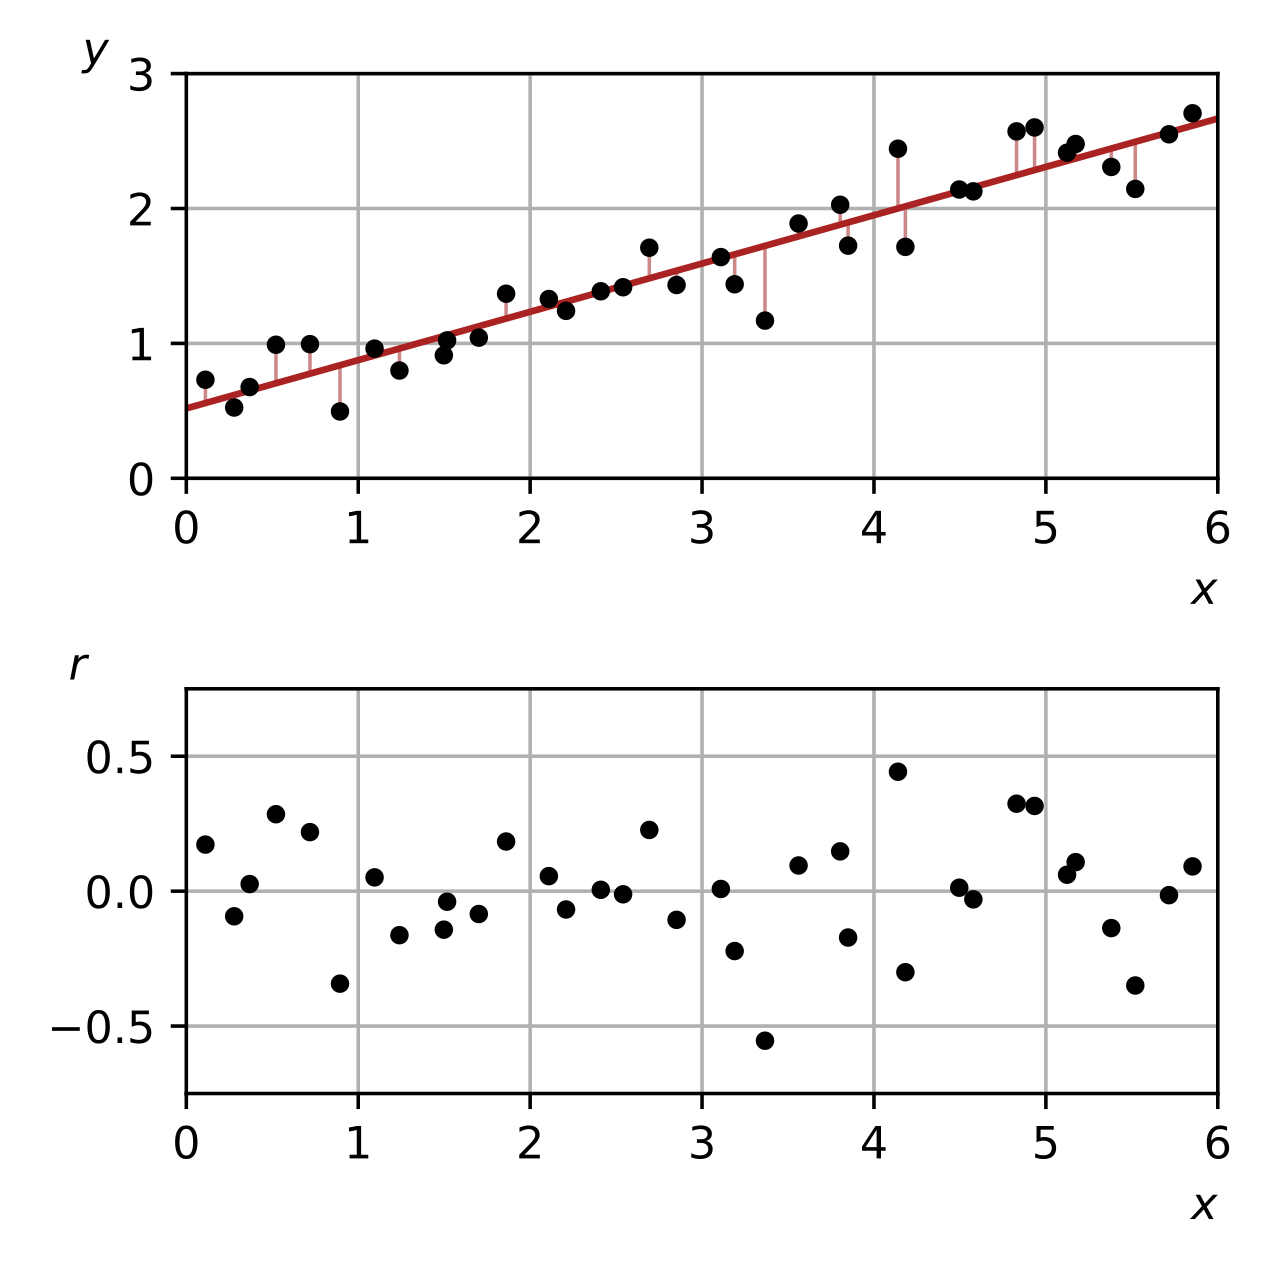
\includegraphics[width=0.78\linewidth]{assets/images/linearni-regrese/linear-regression-residuals.png}
  \caption[Regresní přímka a rezidua]{Regresní přímka a reziduální graf. Popis obrázku: horní panel
  ukazuje body a odhadnutou lineární regresi, dolní panel zobrazuje rezidua vůči vysvětlující proměnné.
  Pokud jsou rezidua náhodně rozptýlená kolem nuly bez systematického vzoru, je lineární specifikace
  věcně přijatelnější. Zdroj obrázku: Justinkunimune,
  \href{https://commons.wikimedia.org/wiki/File:Linear\_regression\_residuals.svg}{Wikimedia Commons},
  licence CC0 1.0.}
  \label{fig:linear-regression-residuals}
\end{figure}

\subsection{Normální rovnice a vlastnosti reziduí}

Z podmínek prvního řádu dostaneme:
\[
X^\top \hat u = 0.
\]

To znamená, že rezidua jsou v odhadnutém modelu nekorelovaná s každou vysvětlující proměnnou zahrnutou
v modelu.

Pokud model obsahuje konstantu, platí také:
\[
\sum_{i=1}^n \hat u_i = 0.
\]

Tedy průměr reziduí je nula.

\subsection{Předpoklady lineárního regresního modelu}

\subsubsection{Linearita v parametrech}

Model je lineární v koeficientech:
\[
y_i = \beta_0+\beta_1x_{i1}+\cdots+\beta_kx_{ik}+u_i.
\]

Proměnné ale mohou být transformované. Model je stále lineární, pokud je lineární v parametrech:
\[
y = \beta_0+\beta_1x+\beta_2x^2+u.
\]

Tento model je lineární v $\beta$, i když vztah mezi $x$ a $y$ je nelineární.

\paragraph{Při porušení.}
Pokud má model špatný funkční tvar, neodpovídá správně podmíněné střední hodnotě
\(\mathrm{E}(y|X)\). OLS potom odhaduje jen nejlepší lineární aproximaci ve vzorku, v reziduích může
zůstávat systematický vzor a koeficienty mohou být vychýlené vůči zamýšlenému efektu, zejména když
chybějící nelineární člen souvisí se zahrnutými regresory. Prakticky se kontrolují reziduální grafy a
podle věcného smyslu se přidávají logaritmy, kvadratické členy, interakce nebo jiné transformace.

\subsubsection{Náhodný výběr}

Pozorování by měla být náhodně vybraná z populace. U průřezových dat se obvykle předpokládá, že jednotky
jsou nezávislé.

\paragraph{Při porušení.}
Pokud vzorek nevznikl náhodně nebo je zatížen selekcí, regresní vztah může popisovat jen dostupný vzorek,
ne cílovou populaci. Jestliže výběr souvisí s nevysvětlenou složkou \(u\), vzniká selection bias a OLS
může být vychýlený. Pokud jsou pozorování závislá, například v klastrech, čase nebo prostoru, samotné
koeficienty nemusí být při exogenitě nutně vychýlené, ale běžné standardní chyby a testy bývají
nespolehlivé. Reakcí jsou výběrové váhy, jasně definovaná cílová populace, klastrované nebo HAC
standardní chyby a modely pro panelová či časová data.

\subsubsection{Žádná perfektní multikolinearita}

Žádná vysvětlující proměnná nesmí být přesnou lineární kombinací ostatních.

\paragraph{Příklad problému.}
Pokud do modelu dáme zároveň všechny dummy proměnné pro kategorie a konstantu, vznikne perfektní
multikolinearita. Proto se jedna kategorie vždy vynechává a slouží jako referenční.

\paragraph{Při porušení.}
Při perfektní multikolinearitě není \(X^\top X\) invertovatelná, takže OLS odhad není jednoznačně
určený. Software typicky některou proměnnou automaticky vyhodí, nebo model vůbec neodhadne. Silná, ale
ne perfektní multikolinearita odhad formálně umožňuje a sama o sobě nezpůsobuje vychýlení, zvyšuje ale
rozptyl odhadů: standardní chyby jsou velké, intervaly spolehlivosti široké a znaménka či velikosti
jednotlivých koeficientů mohou být nestabilní.

\subsubsection{Exogenita}

\[
\mathrm{E}(u|X)=0.
\]

Toto je nejdůležitější předpoklad pro nestrannost a kauzální interpretaci. Znamená, že vysvětlující proměnné
nejsou systematicky spojeny s nepozorovanou složkou $u$.

Porušení exogenity vzniká například při:
\begin{itemize}
    \item vynechané relevantní proměnné,
    \item simultánnosti,
    \item reverzní kauzalitě,
    \item chybě měření ve vysvětlující proměnné.
\end{itemize}

\paragraph{Při porušení.}
OLS je obecně vychýlený a nekonzistentní, takže ani velký vzorek problém automaticky neodstraní.
Koeficient potom směšuje efekt zahrnuté proměnné s vlivem nepozorované složky v chybě a nelze mu dát
kauzální interpretaci. Formálně významný \(t\)-test v takové situaci jen říká, že je odhad přesný kolem
špatného cíle. Typické reakce jsou lepší kontrolní proměnné, proxy proměnné, fixní efekty, instrumentální
proměnné nebo výzkumný design typu difference-in-differences či regression discontinuity.

\subsubsection{Homoskedasticita}

\[
\mathrm{Var}(u|X)=\sigma^2.
\]

Rozptyl chyb je konstantní pro všechny hodnoty $X$.

Pokud rozptyl chyb závisí na $X$, jde o heteroskedasticitu:
\[
\mathrm{Var}(u|X)\neq\sigma^2.
\]

\paragraph{Při porušení.}
Pokud platí exogenita, heteroskedasticita sama o sobě nemusí způsobit vychýlení ani nekonzistenci OLS
koeficientů. Problém je v inferenci: obvyklé standardní chyby, \(t\)-testy, \(F\)-testy, intervaly
spolehlivosti a vlastnost BLUE mohou být špatně. Praktickou reakcí jsou heteroskedasticity-robustní
standardní chyby, vhodná transformace proměnných, vážená metoda nejmenších čtverců nebo lepší
specifikace modelu.

Graficky se často projeví tak, že se rozptyl reziduí systematicky mění s hodnotou vysvětlující proměnné
nebo s predikovanou hodnotou. Typický je \uv{trychtýř}: pro malé hodnoty $x$ jsou rezidua blízko nule,
pro velké hodnoty $x$ se jejich rozptyl zvětšuje.

\begin{figure}[htbp]
  \centering
  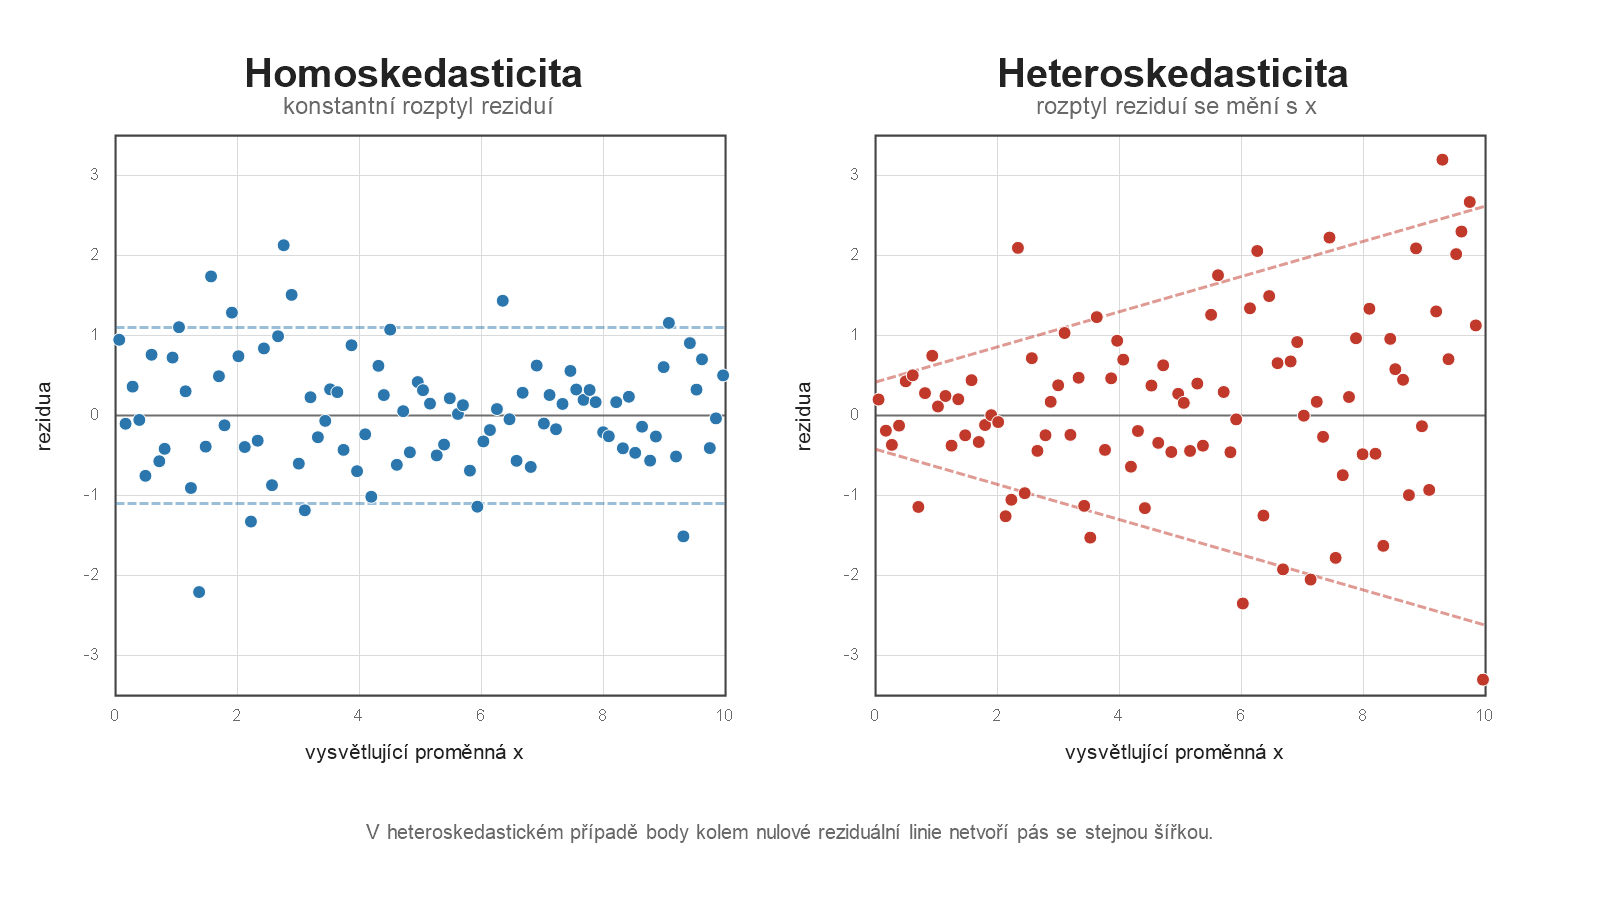
\includegraphics[width=0.95\linewidth]{assets/images/linearni-regrese/homoscedastic-vs-heteroscedastic.png}
  \caption[Homoskedasticita a heteroskedasticita]{Srovnání homoskedasticity a heteroskedasticity v
  reziduálním grafu. Popis obrázku: vlevo mají rezidua přibližně stejný rozptyl pro všechny hodnoty
  $x$, vpravo se rozptyl reziduí s rostoucím $x$ zvětšuje. Zdroj obrázku: vlastní zpracování.}
  \label{fig:homoscedastic-vs-heteroscedastic}
\end{figure}

\subsubsection{Normalita chyb}

\[
u|X \sim N(0,\sigma^2).
\]

Normalita je důležitá hlavně pro přesnou inferenci v malých výběrech. Ve velkých výběrech se často opíráme
o asymptotickou normalitu.

\paragraph{Při porušení.}
Nenormalita chyb sama o sobě nemění vypočtené OLS koeficienty a při splnění ostatních klíčových
předpokladů nebere OLS nestrannost ani konzistenci. V malých vzorcích ale přestávají být přesné klasické
\(t\)-testy, \(F\)-testy, \(p\)-hodnoty a intervaly spolehlivosti odvozené z normality. Ve velkých
vzorcích se používá centrální limitní věta a asymptotická normalita; při těžkých ocasech nebo odlehlých
hodnotách je vhodné zvážit robustní inferenci, bootstrap, transformaci proměnných nebo robustnější
odhadovou metodu.

\paragraph{Zkoušková zkratka.}
LRM.1--LRM.4 jsou klíčové pro nestrannost a konzistenci OLS, LRM.5 přidává obvyklé standardní chyby a
Gaussovu-Markovovu vlastnost BLUE. Normalita chyb není nutná pro velké vzorky, ale dává přesnou
malovýběrovou inferenci.

\subsection{Vlastnosti OLS odhadů}

\subsubsection{Nestrannost}

Pokud platí linearita, náhodný výběr, žádná perfektní multikolinearita a exogenita, potom:
\[
\mathrm{E}(\hat\beta|X)=\beta.
\]

To znamená, že OLS se v průměru trefuje do skutečné hodnoty parametru.

\subsubsection{Konzistence}

Odhad je konzistentní, pokud se s rostoucím počtem pozorování přibližuje ke skutečné hodnotě:
\[
\operatorname{plim}\hat\beta=\beta.
\]

Konzistence je slabší než nestrannost. Odhad může být v malém vzorku vychýlený, ale pokud se s rostoucím
$n$ blíží ke skutečné hodnotě, je konzistentní.

\subsubsection{Rozptyl OLS}

Za homoskedasticity:
\[
\mathrm{Var}(\hat\beta|X)=\sigma^2(X^\top X)^{-1}.
\]

Odhad rozptylu chyb:
\[
\hat\sigma^2 = \frac{SSR}{n-k-1}.
\]

\subsubsection{Gaussova-Markovova věta}

Pokud platí předpoklady LRM včetně homoskedasticity, je OLS:
\[
BLUE = \text{Best Linear Unbiased Estimator}.
\]

To znamená, že mezi lineárními nestrannými odhady má nejmenší rozptyl.

\paragraph{Pozor.}
BLUE neznamená, že OLS je vždy nejlepší možný odhad mezi všemi odhady. Znamená to nejlepší mezi
\emph{lineárními nestrannými} odhady za daných předpokladů.

\subsection{Statistická inference}

Protože pracujeme se vzorkem, odhady se mezi různými vzorky liší. Standardní chyba říká, jak moc je odhad
nejistý:
\[
se(\hat\beta_j).
\]

\subsubsection{t-test jednoho koeficientu}

Testujeme:
\[
H_0:\beta_j=0
\]
proti
\[
H_1:\beta_j\neq 0.
\]

Testová statistika:
\[
t=
\frac{\hat\beta_j-\beta_{j,0}}{se(\hat\beta_j)}.
\]

Nejčastěji:
\[
t=
\frac{\hat\beta_j}{se(\hat\beta_j)}.
\]

Pokud je $|t|$ velké, zamítáme nulovou hypotézu.

Intuice: t-test porovnává \term{velikost odhadu} s \term{nejistotou odhadu}. Koeficient může být věcně
velký, ale pokud má ještě větší standardní chybu, nemáme dost důkazů, že se skutečný populační koeficient
liší od testované hodnoty. Naopak i malý koeficient může být statisticky významný, pokud je odhadnutý
velmi přesně.

\(\beta_{j,0}\) je hodnota koeficientu pod nulovou hypotézou. Nejčastěji testujeme \(\beta_{j,0}=0\),
tedy otázku:
\[
\text{Má proměnná } x_j \text{ při kontrole ostatních proměnných lineární vztah s } y?
\]
Přesněji: test říká, zda je odhadovaný parciální efekt statisticky odlišný od nuly, ne zda je efekt
kauzální, důležitý nebo ekonomicky velký.

Za klasických předpokladů lineárního regresního modelu má testová statistika při platnosti \(H_0\)
t-rozdělení s
\[
n-k-1
\]
stupni volnosti, kde \(n\) je počet pozorování a \(k\) počet vysvětlujících proměnných bez konstanty.
Ve velkých vzorcích se t-rozdělení blíží normálnímu rozdělení, proto se často používá hranice přibližně
\(1.96\) pro oboustranný 5\% test.

\paragraph{p-hodnota.}
p-hodnota říká, jak extrémní t-statistiku bychom dostali, pokud by nulová hypotéza byla pravdivá. Pro
oboustranný test zamítáme \(H_0\) na hladině významnosti \(\alpha\), pokud:
\[
p < \alpha.
\]
Například při \(\alpha=0.05\) zamítáme nulovou hypotézu, pokud je p-hodnota menší než 0.05.

\paragraph{Příklad.}
Odhadneme koeficient u proměnné \(educ\):
\[
\hat\beta_{educ}=1200,
\qquad
se(\hat\beta_{educ})=400.
\]
Test nulové hypotézy \(H_0:\beta_{educ}=0\):
\[
t=\frac{1200-0}{400}=3.
\]
Koeficient je tři standardní chyby od nuly. V běžném velkém vzorku by to znamenalo statisticky významný
výsledek na 5\% hladině. Interpretace ale není \uv{vzdělání určitě kauzálně zvyšuje mzdu o 1200}.
Správnější je: při dané specifikaci modelu je odhadovaný parciální vztah mezi vzděláním a mzdou
statisticky odlišný od nuly.

\paragraph{Pozor na předpoklady.}
Pokud je v modelu heteroskedasticita nebo autokorelace, běžné standardní chyby mohou být špatně odhadnuté
a t-test může zamítat příliš často nebo příliš málo. V takové situaci se obvykle používají robustní
standardní chyby. Pokud je porušena exogenita, t-test může být formálně významný, ale koeficient nemá
čistou kauzální interpretaci.

\subsubsection{Interval spolehlivosti}

\[
\hat\beta_j \pm c \cdot se(\hat\beta_j).
\]

Přibližně pro 95\% interval ve velkém výběru:
\[
\hat\beta_j \pm 1.96 \cdot se(\hat\beta_j).
\]

Interval spolehlivosti ukazuje rozsah hodnot parametru, které jsou s daty a modelem rozumně slučitelné.
U 95\% intervalu neříkáme, že konkrétní interval obsahuje skutečný parametr s pravděpodobností 95\%.
Přesnější interpretace je: kdybychom opakovaně vybírali vzorky a pro každý spočítali interval stejným
postupem, přibližně 95\% takových intervalů by obsahovalo skutečnou hodnotu \(\beta_j\).

Souvislost s t-testem: pokud 95\% interval pro \(\beta_j\) neobsahuje nulu, oboustranný t-test
\(H_0:\beta_j=0\) obvykle zamítne na 5\% hladině. Širší interval znamená větší nejistotu odhadu,
užší interval přesnější odhad.

\subsubsection{F-test více omezení}

Používá se, když testujeme více koeficientů najednou, například:
\[
H_0:\beta_2=\beta_3=\beta_4=0.
\]

F-statistika:
\[
F=
\frac{(SSR_r-SSR_u)/m}{SSR_u/(n-k-1)}.
\]

Kde:
\begin{itemize}
    \item $SSR_r$ je součet čtverců reziduí v restriktivním modelu,
    \item $SSR_u$ je součet čtverců reziduí v neresktriktivním modelu,
    \item $m$ je počet testovaných restrikcí.
\end{itemize}

Restriktivní model vynucuje nulovou hypotézu, například vynechá proměnné \(x_2,x_3,x_4\). Neresktriktivní
model je plný model, kde tyto koeficienty odhadujeme volně. F-test tedy porovnává, jak moc se zhorší fit,
když daná omezení vynutíme.

Intuice: pokud vynechání testovaných proměnných výrazně zvýší reziduální součet čtverců, omezení jsou
pro data nevěrohodná a \(H_0\) zamítáme. F-test je vhodný pro otázky typu \uv{mají tyto proměnné jako
skupina nějaký význam?}. Jednotlivé t-testy by zde nestačily, protože neodpovídají přímo na společnou
hypotézu a zvyšují riziko chyb při opakovaném testování.

\subsection{Dobrota shody}

Celková variabilita:
\[
SST=\sum_{i=1}^n (y_i-\bar y)^2.
\]

\(SST\) měří, jak moc se skutečné hodnoty \(y_i\) celkově liší od svého průměru \(\bar y\). Je to
variabilita, kterou se model snaží vysvětlit.

Nevysvětlená variabilita:
\[
SSR=\sum_{i=1}^n \hat u_i^2.
\]

\(SSR\) zde znamená reziduální součet čtverců, tedy část variability, kterou model nevysvětlil:
\[
\hat u_i = y_i-\hat y_i.
\]
Čím jsou body blíže regresní přímce, tím menší je \(SSR\). V některých učebnicích se stejná veličina
značí \(RSS\) nebo \(SSE\).

U lineární regrese s konstantou platí rozklad:
\[
SST
=
\sum_{i=1}^n(\hat y_i-\bar y)^2
+
\sum_{i=1}^n(y_i-\hat y_i)^2.
\]
Tedy:
\[
\text{celková variabilita}
=
\text{vysvětlená variabilita}
+
\text{nevysvětlená variabilita}.
\]

Koeficient determinace:
\[
R^2=1-\frac{SSR}{SST}.
\]

\(R^2\) říká, jakou část variability \(y\) model vysvětluje. Ekvivalentně:
\[
R^2=
\frac{\text{vysvětlená variabilita}}{\text{celková variabilita}}.
\]
Například pokud \(SST=100\) a \(SSR=25\), potom:
\[
R^2=1-\frac{25}{100}=0.75.
\]
Model tedy vysvětluje 75\% variability \(y\) kolem průměru a 25\% zůstává v reziduích.

\begin{figure}[htbp]
  \centering
  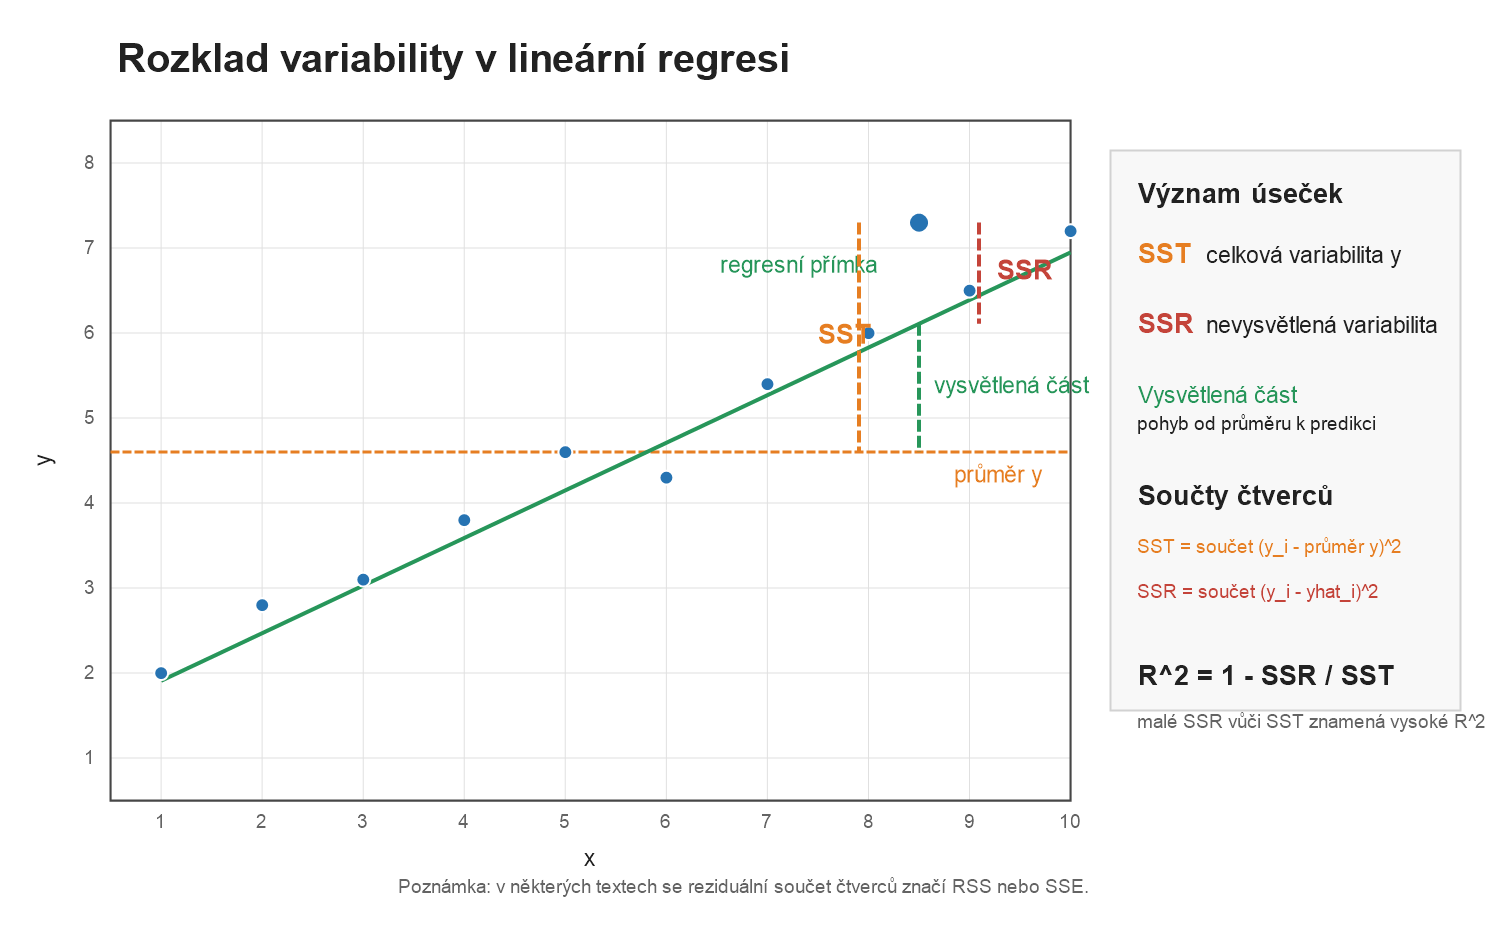
\includegraphics[width=0.95\linewidth]{assets/images/linearni-regrese/r-squared-sst-ssr.png}
  \caption[Rozklad variability v regresi]{Rozklad variability závisle proměnné v lineární regresi.
  Popis obrázku: oranžová úsečka ukazuje celkovou odchylku pozorování od průměru, červená reziduální
  odchylku od regresní přímky a zelená vysvětlenou část mezi průměrem a predikcí. Zdroj obrázku:
  vlastní zpracování.}
  \label{fig:linear-regression-sums-of-squares}
\end{figure}

\paragraph{Pozor.}
Vyšší $R^2$ neznamená automaticky lepší model pro kauzální interpretaci. Model může mít vysoké $R^2$,
ale být špatně specifikovaný nebo trpět endogenitou.

Adjusted $R^2$ penalizuje počet proměnných:
\[
\bar R^2
=
1-
\frac{SSR/(n-k-1)}{SST/(n-1)}.
\]

\subsection{Predikce}

Bodová predikce:
\[
\hat y_0=x_0^\top\hat\beta.
\]

Je důležité rozlišovat dva typy nejistoty:

\begin{itemize}
    \item interval spolehlivosti pro průměrnou hodnotu $\mathrm{E}(y|x_0)$,
    \item predikční interval pro konkrétní nové pozorování $y_0$.
\end{itemize}

Predikční interval je širší, protože obsahuje:
\begin{itemize}
    \item nejistotu v odhadu regresní funkce,
    \item náhodnou individuální odchylku $u$.
\end{itemize}

Přibližně:
\[
\hat y_0
\pm
c
\sqrt{
x_0^\top \widehat{\mathrm{Var}}(\hat\beta)x_0
+
\hat\sigma^2
}.
\]

\begin{figure}[htbp]
  \centering
  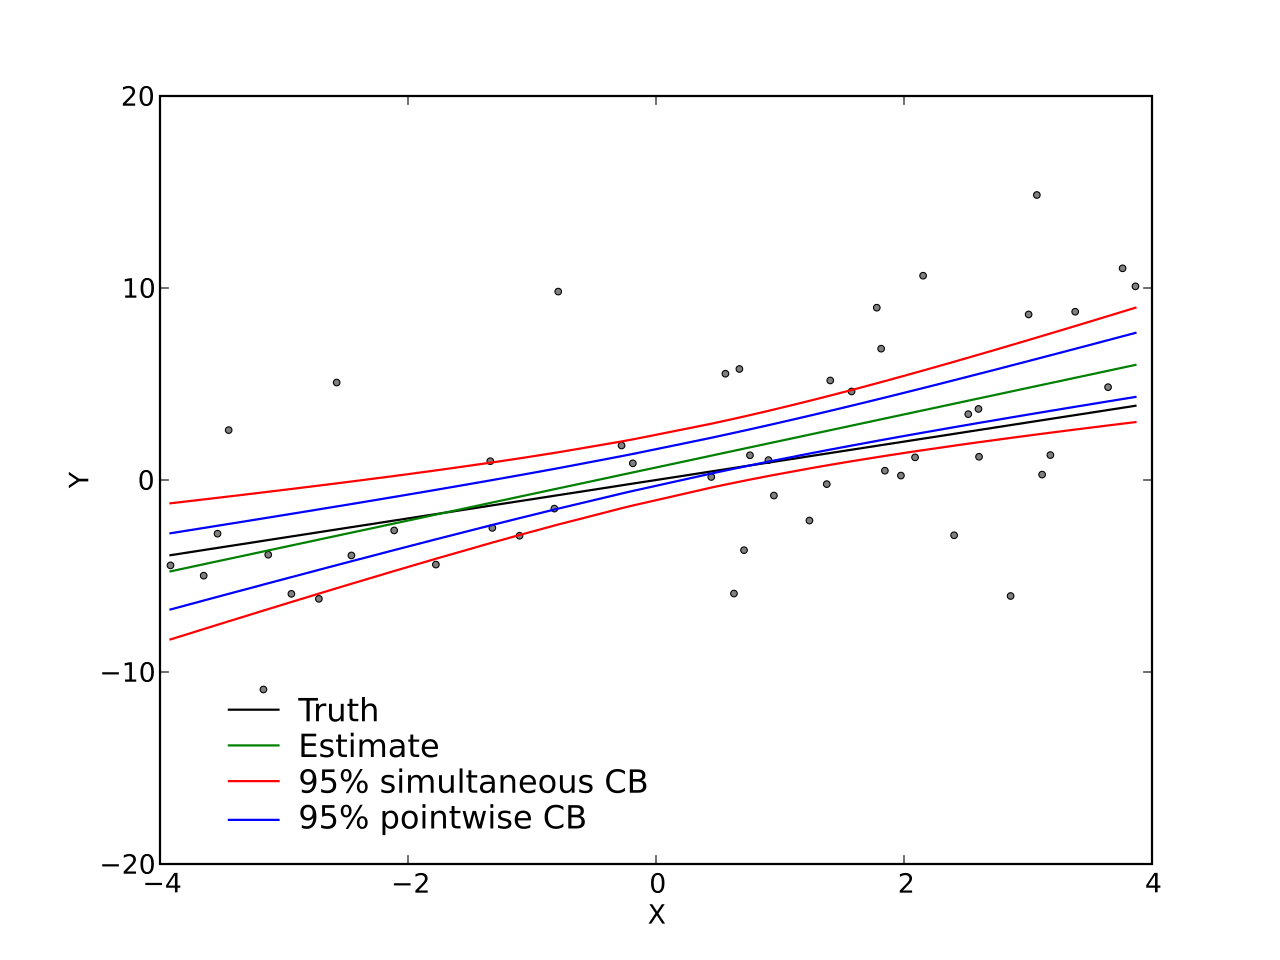
\includegraphics[width=0.82\linewidth]{assets/images/linearni-regrese/regression-confidence-band.png}
  \caption[Regresní nejistota]{Odhadnutá regresní funkce a pásy nejistoty. Popis obrázku: zelená
  křivka je odhad, modré a červené pásy ukazují různé typy konfidenčních pásem kolem regresní funkce.
  Pásy se typicky rozšiřují dál od středu dat, kde je odhad méně opřený o pozorování. Zdroj obrázku:
  Skbkekas, \href{https://commons.wikimedia.org/wiki/File:Regression\_confidence\_band.svg}{Wikimedia Commons},
  licence CC BY 3.0.}
  \label{fig:regression-confidence-band}
\end{figure}

\paragraph{Extrapolace.}
Regrese predikuje nejspolehlivěji v oblasti hodnot, které jsou podobné trénovacím datům. Predikce mimo
pozorovaný rozsah $x$ je extrapolace a může být zavádějící i tehdy, když má model v trénovacích datech
vysoké $R^2$.

\subsection{Volba modelu}

Při volbě modelu řešíme:
\begin{itemize}
    \item které proměnné zahrnout,
    \item jak je transformovat,
    \item zda zahrnout interakce,
    \item zda vztah není nelineární,
    \item zda model slouží k popisu, predikci nebo kauzalitě.
\end{itemize}

\subsubsection{Volba podle účelu}

\begin{itemize}
    \item \textbf{Deskriptivní model} má přehledně popsat vztahy v datech. Důležitá je srozumitelná
    interpretace koeficientů a transparentní specifikace.
    \item \textbf{Prediktivní model} vybíráme podle chyby na validačních nebo testovacích datech.
    Může obsahovat proměnné, které zlepšují predikci, i když nemají čistou kauzální interpretaci.
    \item \textbf{Kauzální model} stavíme kolem identifikační otázky. Klíčové je zahrnout relevantní
    confoundery, vyhnout se špatným kontrolním proměnným a obhájit exogenitu.
\end{itemize}

Proto neexistuje jeden univerzálně \uv{nejlepší} regresní model. Model s nejvyšším $R^2$ nemusí být
nejlepší pro predikci mimo trénovací data a už vůbec nemusí identifikovat kauzální efekt.

\subsubsection{Křížová validace, informační kritéria a regularizace}
U prediktivních úloh se model volí podle výkonu mimo trénovací data. \term{Holdout} rozdělí data na
trénovací, validační a testovací část. \term{k-fold cross-validation} rozdělí data na \(k\) částí,
model vždy trénuje na \(k-1\) částech a testuje na zbývající části; výsledná chyba je průměr přes
všechny foldy. Testovací množina se používá až na konečné nezávislé vyhodnocení.

\term{AIC} a \term{BIC} porovnávají modely pomocí věrohodnosti penalizované za počet parametrů.
Nižší hodnota znamená lepší kompromis mezi shodou s daty a složitostí. AIC obvykle penalizuje
složitost mírněji, BIC přísněji, protože penalizace roste s velikostí vzorku. U lineární regrese se
často sleduje také adjustované \(R^2\), které na rozdíl od běžného \(R^2\) trestá zbytečné proměnné.

\term{Ridge} regrese používá \(L_2\) penalizaci:
\[
  \min_\beta \sum_{i=1}^n (y_i-x_i^\top\beta)^2 + \lambda \sum_{j=1}^p \beta_j^2.
\]
Koeficienty zmenšuje směrem k nule, ale obvykle je nenastaví přesně na nulu. Hodí se při multikolinearitě
a v situacích, kdy mnoho proměnných nese malou část signálu.

\term{LASSO} používá \(L_1\) penalizaci:
\[
  \min_\beta \sum_{i=1}^n (y_i-x_i^\top\beta)^2 + \lambda \sum_{j=1}^p |\beta_j|.
\]
Může některé koeficienty nastavit přesně na nulu, takže funguje jako výběr proměnných. Pokud jsou ale
prediktory silně korelované, může vybrat jen jeden z několika podobných prediktorů.

\term{Elastic net} kombinuje \(L_1\) a \(L_2\) penalizaci. Prakticky je užitečný, když chceme zároveň
stabilizovat odhady a provádět výběr proměnných.

U všech penalizovaných regresí je zásadní \term{škálování prediktorů}. Penalizace působí na velikost
koeficientů, takže proměnná měřená v korunách, tisících korun nebo procentech by bez standardizace
dostala jiný trest. Proto se numerické prediktory typicky standardizují a parametr \(\lambda\) se volí
pomocí validačních dat nebo křížové validace. Intercept se obvykle nepenalizuje.

\subsubsection{Dummy proměnné}

Kategoriální proměnné se do regrese dávají pomocí dummy proměnných.

Pokud má proměnná tři kategorie, například:
\[
\text{Felicia, Octavia, Superb},
\]
vložíme do modelu jen dvě dummy proměnné. Jedna kategorie je referenční.

Příklad:
\[
price = \beta_0+\beta_1 km+\beta_2 year+\beta_3 Octavia+\beta_4 Superb+u.
\]

Pokud je referenční kategorie Felicia, potom:
\begin{itemize}
    \item $\beta_3$ říká, o kolik se liší Octavia od Felicie při stejném $km$ a $year$,
    \item $\beta_4$ říká, o kolik se liší Superb od Felicie při stejném $km$ a $year$.
\end{itemize}

\subsubsection{Logaritmické transformace}

Model:
\[
\log(y)=\beta_0+\beta_1x+u.
\]

Interpretace:
\[
100\beta_1
\]
je přibližná procentní změna $y$ při jednotkové změně $x$.

Přesná procentní změna:
\[
100(e^{\beta_1}-1).
\]

Model:
\[
\log(y)=\beta_0+\beta_1\log(x)+u.
\]

Zde je $\beta_1$ elasticita:
\[
1\% \text{ změna } x
\quad \Rightarrow \quad
\beta_1\% \text{ změna } y.
\]

\paragraph{Logaritmus a kvantilové kódování.}
Logaritmus je pro kladné hodnoty monotónní transformace. Nemění pořadí pozorování, takže pokud se
kategorie tvoří jen podle kvantilů téže proměnné, stejné jednotky zůstanou ve stejných kvantilových
skupinách. Změní se ale vzdálenosti mezi hodnotami a interpretace rozdílů, což může být důležité pro
regresi nebo metody citlivé na měřítko.

\subsubsection{Kvadratický člen}

Pokud vztah není lineární, můžeme přidat $x^2$:
\[
y=\beta_0+\beta_1x+\beta_2x^2+u.
\]

Marginální efekt:
\[
\frac{\partial \mathrm{E}(y|x)}{\partial x}
=
\beta_1+2\beta_2x.
\]

Bod obratu:
\[
x^*=-\frac{\beta_1}{2\beta_2}.
\]

\subsubsection{Interakce}

Interakce znamená, že efekt jedné proměnné závisí na hodnotě jiné proměnné:
\[
y=\beta_0+\beta_1x+\beta_2z+\beta_3xz+u.
\]

Efekt $x$:
\[
\frac{\partial \mathrm{E}(y|x,z)}{\partial x}
=
\beta_1+\beta_3z.
\]

\paragraph{Příklad.}
Efekt vzdělání na mzdu se může lišit podle pohlaví. Potom do modelu přidáme interakci:
\[
wage=\beta_0+\beta_1educ+\beta_2female+\beta_3(educ\cdot female)+u.
\]

\subsection{Vynechaná proměnná a omitted variable bias}

Skutečný model:
\[
y=\beta_0+\beta_1x+\gamma z+u.
\]

Pokud ale odhadneme model bez $z$:
\[
y=\alpha_0+\alpha_1x+v,
\]
může vzniknout vychýlení.

Vzorec pro omitted variable bias:
\[
\operatorname{plim}(\tilde\beta_1)
=
\beta_1
+
\gamma\frac{\mathrm{Cov}(x,z)}{\mathrm{Var}(x)}.
\]

Bias vzniká, pokud platí obě podmínky:
\begin{itemize}
    \item $z$ ovlivňuje $y$, tedy $\gamma\neq 0$,
    \item $z$ koreluje s $x$, tedy $\mathrm{Cov}(x,z)\neq 0$.
\end{itemize}

\paragraph{Intuice.}
Pokud vynechaná proměnná souvisí s vysvětlující proměnnou, model její efekt mylně přičte proměnné $x$.

Možné reakce závisí na povaze problému. \term{Proxy proměnná} je pozorovatelná náhrada nepozorovaného
faktoru, například testové skóre jako přibližná kontrola schopností v regresi mzdy na vzdělání.
Proxy se vkládá přímo do rovnice a pomáhá snížit vychýlení, pokud dobře zachycuje vynechaný faktor.
\term{Instrumentální proměnná} se používá, když je vysvětlující proměnná endogenní. Dobrý instrument
musí být relevantní pro endogenní proměnnou a zároveň exogenní vůči chybě v hlavní rovnici. Častým
odhadem je dvoustupňová metoda nejmenších čtverců, zkráceně 2SLS.

\subsection{Multikolinearita}

Multikolinearita znamená, že vysvětlující proměnné jsou mezi sebou silně korelované.

Rozptyl koeficientu:
\[
\mathrm{Var}(\hat\beta_j)
=
\frac{\sigma^2}{SST_j(1-R_j^2)}.
\]

Kde:
\begin{itemize}
    \item $SST_j$ je variabilita proměnné $x_j$,
    \item $R_j^2$ je $R^2$ z pomocné regrese $x_j$ na ostatní vysvětlující proměnné.
\end{itemize}

Variance Inflation Factor:
\[
VIF_j=\frac{1}{1-R_j^2}.
\]

Vysoký $VIF$ znamená, že $x_j$ je silně vysvětlitelná ostatními regresory.

\paragraph{Důsledek.}
Multikolinearita obvykle nezpůsobuje vychýlení, ale zvyšuje standardní chyby. Koeficienty jsou pak
nepřesné, intervaly spolehlivosti široké a proměnné mohou vycházet statisticky nevýznamné.

\subsection{Heteroskedasticita}

Heteroskedasticita:
\[
\mathrm{Var}(u_i|X_i)\neq \sigma^2.
\]

Typicky se objevuje například u příjmových dat, kde lidé s vyšším příjmem mají často větší variabilitu.

\paragraph{Důsledek.}
Pokud platí exogenita, OLS koeficienty mohou být stále nestranné a konzistentní. Problém je ve standardních
chybách:
\[
se(\hat\beta_j)
\]
mohou být špatně odhadnuté.

Řešení:
\begin{itemize}
    \item heteroskedasticity-robust standard errors,
    \item vážené nejmenší čtverce,
    \item vhodná transformace proměnných.
\end{itemize}

\begin{figure}[htbp]
  \centering
  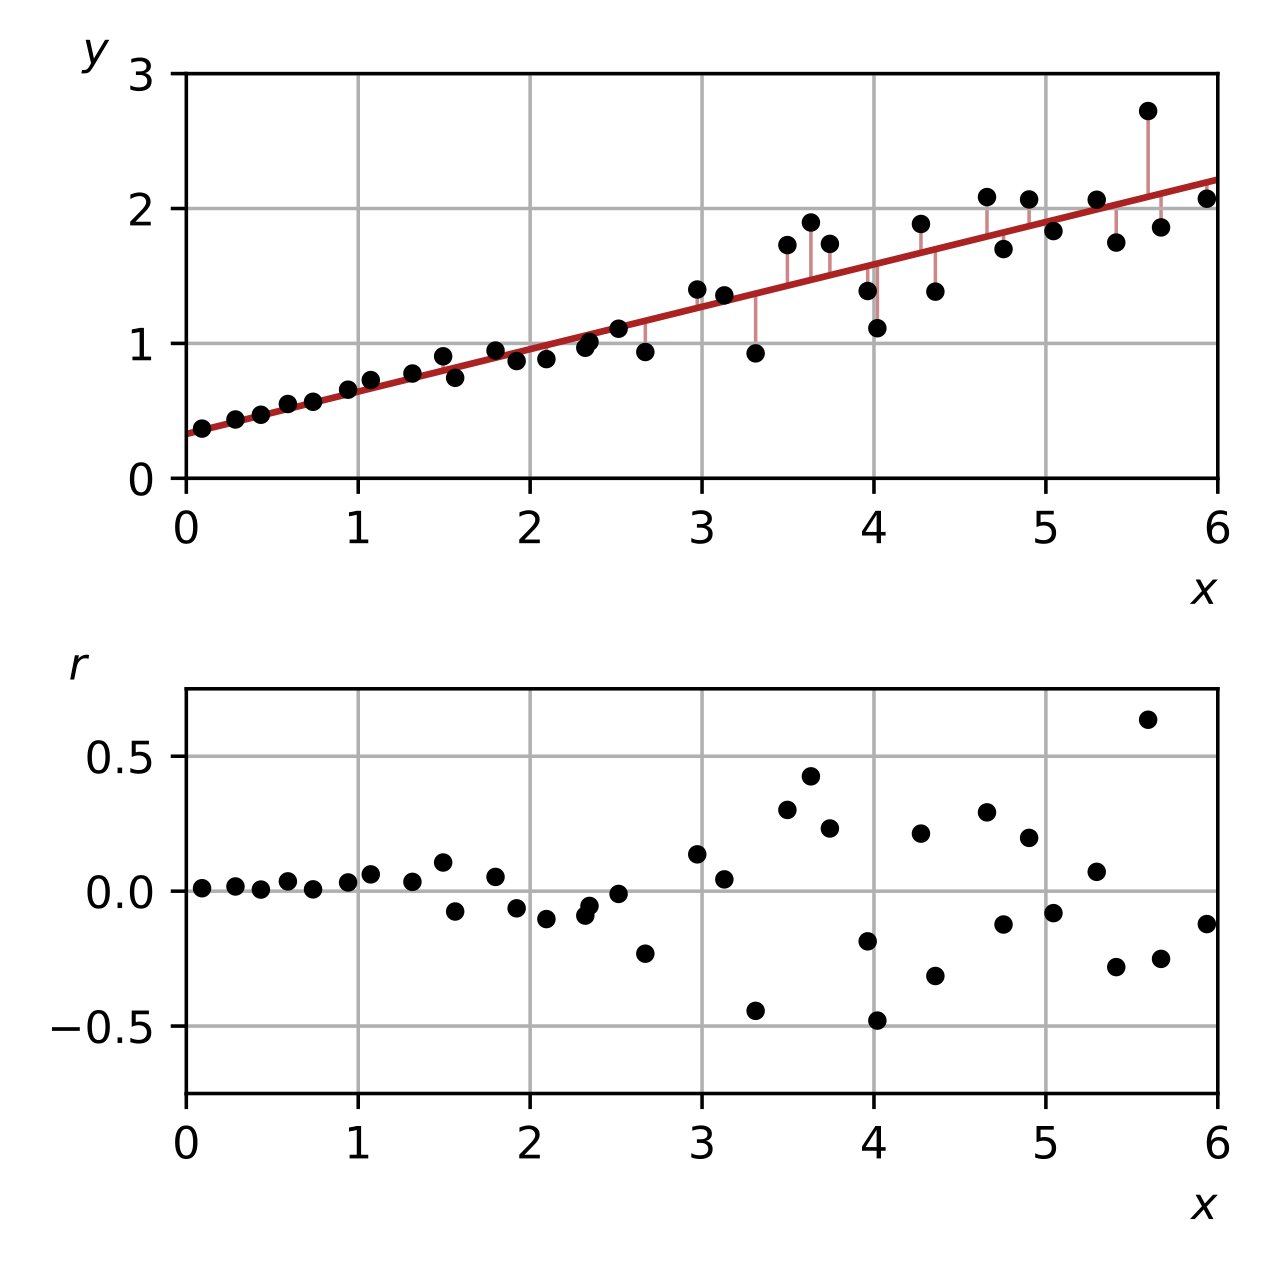
\includegraphics[width=0.78\linewidth]{assets/images/linearni-regrese/heteroscedastic-residuals.png}
  \caption[Heteroskedasticita v reziduích]{Reziduální graf s heteroskedasticitou. Popis obrázku:
  horní panel ukazuje lineární regresi, dolní panel ukazuje, že rozptyl reziduí není konstantní, ale
  roste s hodnotou vysvětlující proměnné. V takové situaci je potřeba řešit zejména správné
  standardní chyby a inferenci. Zdroj obrázku: Justinkunimune,
  \href{https://commons.wikimedia.org/wiki/File:Linear\_regression\_residuals\_heteroscedastic.svg}{Wikimedia Commons},
  licence CC0 1.0.}
  \label{fig:heteroscedastic-residuals}
\end{figure}

\subsection{Diagnostika regresního modelu}

Po odhadu nestačí opsat tabulku koeficientů. Je potřeba ověřit, zda model odpovídá účelu analýzy.

Typicky kontrolujeme:
\begin{itemize}
    \item \textbf{rezidua vs. fitted values} -- vzor v reziduích může znamenat nelinearitu,
    heteroskedasticitu nebo chybějící proměnné;
    \item \textbf{odlehlá a vlivná pozorování} -- extrémy mohou výrazně změnit koeficienty;
    \item \textbf{multikolinearitu} -- vysoké VIF a široké intervaly spolehlivosti u klíčových
    proměnných;
    \item \textbf{normalitu reziduí} -- hlavně pro malovýběrovou inferenci;
    \item \textbf{predikční výkon} -- u prediktivních úloh validační/testovací chyba, například RMSE
    nebo MAE;
    \item \textbf{věcnou plausibilitu} -- znaménka, velikosti efektů a jednotky musejí dávat ekonomický
    smysl.
\end{itemize}

\subsection{Pozor u zkoušky}

Nejčastější chyba je zaměnit statistickou významnost za věcnou nebo kauzální významnost. Malé
$p$-value říká, že odhad je vzhledem ke standardní chybě vzdálený od nulové hypotézy, ne že efekt je
velký, důležitý nebo kauzální. Druhá častá chyba je tvrdit, že vysoké $R^2$ znamená správný model.
Pro kauzalitu je důležitá exogenita a argument o tom, proč v chybě nezůstává confounder. Pro predikci je
důležitá chyba na nových datech, ne jen fit v trénovacím souboru.

\subsection{Shrnutí ke zkoušce}

Lineární regrese modeluje podmíněnou střední hodnotu $y$ pomocí lineární kombinace vysvětlujících
proměnných. OLS minimalizuje součet čtverců reziduí:
\[
\hat\beta=(X^\top X)^{-1}X^\top y.
\]
Regrese může sloužit k deskripci, predikci i kauzální analýze, ale kauzální interpretace vyžaduje především
exogenitu:
\[
\mathrm{E}(u|X)=0.
\]
Při splnění základních předpokladů je OLS nestranný a konzistentní; při homoskedasticitě je BLUE.
Při praktickém použití je nutné řešit volbu modelu, vynechané proměnné, multikolinearitu,
heteroskedasticitu a správnou interpretaci koeficientů.

\subsection{Zdroje}
\begin{itemize}
    \item statsmodels User Guide:
    \href{https://www.statsmodels.org/stable/regression.html}{Linear Regression}.
    \item scikit-learn User Guide:
    \href{https://scikit-learn.org/stable/modules/linear\_model.html}{Linear Models}.
    \item PennState Eberly College of Science:
    \href{https://online.stat.psu.edu/stat501/}{STAT 501 -- Regression Methods}.
    \item Zeileis:
    \href{https://cran.r-project.org/web/packages/sandwich/vignettes/sandwich.pdf}{Econometric Computing with HC and HAC Covariance Matrix Estimators}.
    \item Wikimedia Commons:
    \href{https://commons.wikimedia.org/wiki/File:Linear\_regression\_residuals.svg}{File:Linear\_regression\_residuals.svg}.
    \item Wikimedia Commons:
    \href{https://commons.wikimedia.org/wiki/File:Linear\_Regression\_Plot.png}{File:Linear\_Regression\_Plot.png}.
    \item Wikimedia Commons:
    \href{https://commons.wikimedia.org/wiki/File:Regression\_confidence\_band.svg}{File:Regression\_confidence\_band.svg}.
    \item Wikimedia Commons:
    \href{https://commons.wikimedia.org/wiki/File:Linear\_regression\_residuals\_heteroscedastic.svg}{heteroskedastic residual plot}.
\end{itemize}

\newpage

\section{Zobecněné lineární regresní modely. Modely pro binární, multinomickou a čítací závisle proměnnou}

\subsection{Motivace}

Klasická lineární regrese je vhodná hlavně tehdy, když je závisle proměnná přibližně spojitá a není omezena
na malý počet hodnot. Pro mnoho ekonomických a sociálních dat to ale neplatí.

Typické příklady:
\begin{itemize}
    \item binární proměnná: zaměstnaný / nezaměstnaný,
    \item kategoriální proměnná: volba značky, politické strany nebo dopravního prostředku,
    \item čítací proměnná: počet návštěv lékaře, počet nákupů, počet nehod,
    \item cenzorovaná proměnná: mzda oříznutá shora nebo výdaje s mnoha nulami.
\end{itemize}

V takových situacích se používají zobecněné lineární modely nebo modely s omezenou závisle proměnnou.

\subsection{Obecný rámec GLM}

U zobecněného lineárního modelu rozlišujeme:
\[
\mu_i=\mathrm{E}(y_i|x_i),
\]
a lineární prediktor:
\[
\eta_i=x_i^\top\beta.
\]

GLM spojuje střední hodnotu $\mu_i$ s lineárním prediktorem pomocí link funkce:
\[
g(\mu_i)=x_i^\top\beta.
\]

Kde:
\begin{itemize}
    \item $g(\cdot)$ je link funkce,
    \item $\mu_i$ je podmíněná střední hodnota,
    \item $x_i^\top\beta$ je lineární index.
\end{itemize}

\paragraph{Intuice.}
Nechceme nutně modelovat $y$ přímo jako lineární funkci $x$. Místo toho modelujeme vhodnou transformaci
střední hodnoty. Například u binární proměnné nechceme, aby predikovaná pravděpodobnost byla menší než 0
nebo větší než 1. Proto použijeme link funkci, která to zajistí.

Parametry se většinou odhadují metodou maximální věrohodnosti:
\[
\hat\beta = \arg\max_{\beta}\ell(\beta).
\]

\subsection{Binární závisle proměnná}

Binární proměnná nabývá pouze hodnot:
\[
y_i\in\{0,1\}.
\]

Například:
\[
y_i=
\begin{cases}
1, & \text{pokud je osoba nezaměstnaná},\\
0, & \text{jinak}.
\end{cases}
\]

Cílem je modelovat pravděpodobnost:
\[
p_i=P(y_i=1|x_i).
\]

\subsection{Lineární pravděpodobnostní model}

Nejjednodušší model pro binární $y$ je lineární pravděpodobnostní model:
\[
P(y_i=1|x_i)=\beta_0+\beta_1x_{i1}+\cdots+\beta_kx_{ik}.
\]

Tedy:
\[
p_i=x_i^\top\beta.
\]

\paragraph{Interpretace.}
Koeficient $\beta_j$ říká, o kolik se změní pravděpodobnost úspěchu při jednotkové změně $x_j$:
\[
\Delta P(y=1|x)=\beta_j\Delta x_j.
\]

Pokud $\beta_j=0.05$, pak jednotkové zvýšení $x_j$ zvyšuje pravděpodobnost o 0.05, tedy o 5 procentních
bodů.

\subsubsection{Výhody LPM}

\begin{itemize}
    \item jednoduchý odhad pomocí OLS,
    \item jednoduchá interpretace koeficientů,
    \item dobrý základní model pro rychlou analýzu.
\end{itemize}

\subsubsection{Nevýhody LPM}

LPM má dvě hlavní nevýhody.

Za prvé, predikované pravděpodobnosti mohou být mimo interval $[0,1]$:
\[
\hat p_i < 0
\quad \text{nebo} \quad
\hat p_i > 1.
\]

To nedává smysl, protože pravděpodobnost nemůže být záporná ani větší než jedna.

Za druhé, model je automaticky heteroskedastický. Pro binární proměnnou platí:
\[
\mathrm{Var}(y_i|x_i)=p_i(1-p_i).
\]

Protože $p_i$ závisí na $x_i$, závisí na $x_i$ i rozptyl.

\paragraph{Řešení.}
U LPM je vhodné používat robustní standardní chyby. Ještě lepší je často použít logit nebo probit.

\subsection{Logit a probit}

Logit a probit modelují pravděpodobnost pomocí nelineární funkce:
\[
P(y_i=1|x_i)=F(x_i^\top\beta).
\]

Funkce $F$ zajišťuje, že výsledek vždy leží mezi 0 a 1:
\[
0<F(x_i^\top\beta)<1.
\]

\subsubsection{Logit}

U logitu:
\[
F(z)=\Lambda(z)=\frac{1}{1+e^{-z}}.
\]

Tedy:
\[
P(y_i=1|x_i)
=
\frac{1}{1+e^{-x_i^\top\beta}}.
\]

\begin{figure}[htbp]
  \centering
  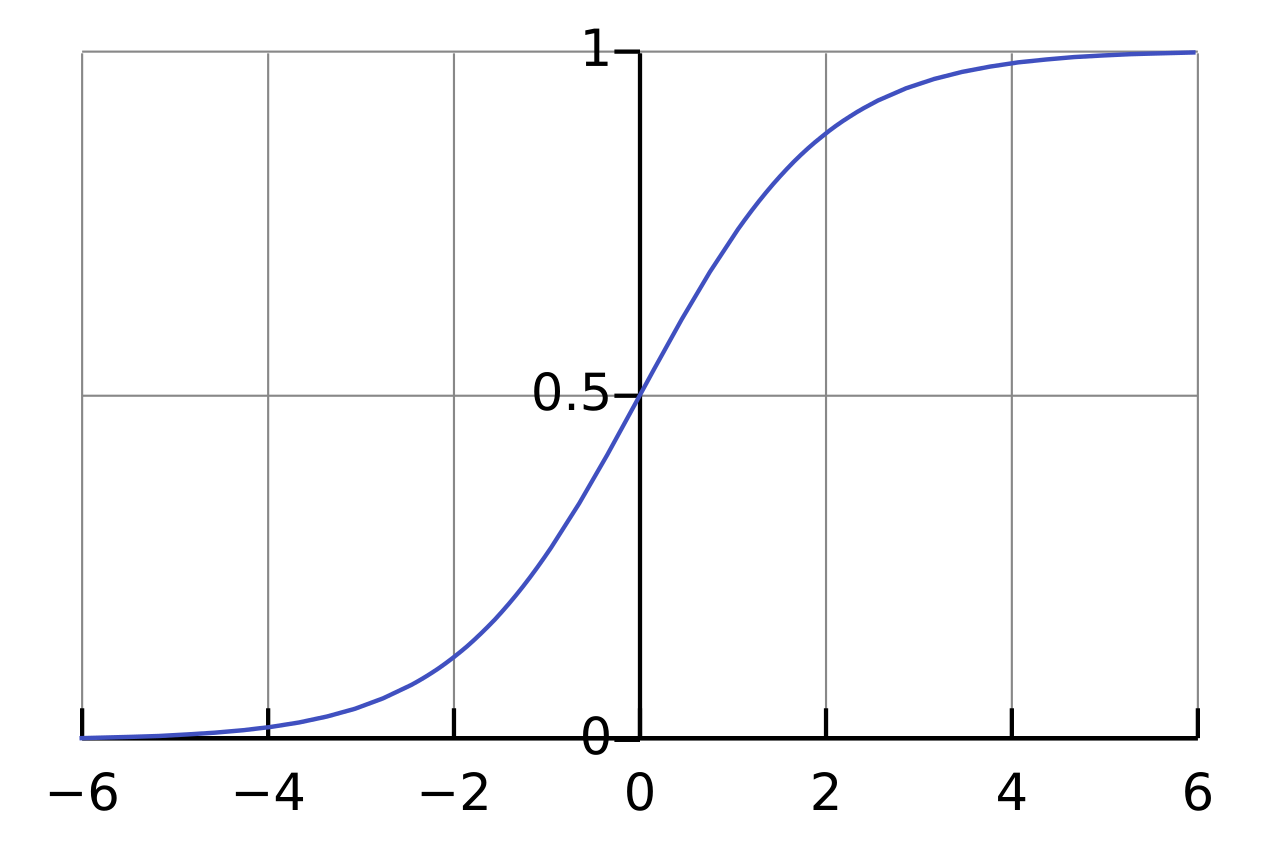
\includegraphics[width=0.72\linewidth]{assets/images/zobecnene-linearni-modely/logistic-curve.png}
  \caption[Logistická funkce]{Logistická funkce používaná v logitu. Popis obrázku: S-křivka převádí
  lineární index $x_i^\top\beta$ na hodnotu mezi 0 a 1, tedy na predikovanou pravděpodobnost úspěchu.
  Největší změna pravděpodobnosti nastává kolem středu křivky, kde je $p$ blízko 0.5. Zdroj obrázku:
  Qef, \href{https://commons.wikimedia.org/wiki/File:Logistic-curve.svg}{Wikimedia Commons},
  licence public domain.}
  \label{fig:logistic-curve}
\end{figure}

\subsubsection{Probit}

U probitu:
\[
F(z)=\Phi(z),
\]
kde $\Phi$ je distribuční funkce standardního normálního rozdělení.

\[
P(y_i=1|x_i)=\Phi(x_i^\top\beta).
\]

\subsection{Latentní interpretace logitu a probitu}

Logit a probit lze chápat přes latentní, tedy nepozorovanou, proměnnou:
\[
y_i^*=x_i^\top\beta+u_i.
\]

Pozorujeme pouze:
\[
y_i=
\begin{cases}
1, & y_i^*>0,\\
0, & y_i^*\leq 0.
\end{cases}
\]

\paragraph{Intuice.}
Například rozhodnutí stát se podnikatelem závisí na nepozorované bilanci výhod a nevýhod.
Pokud latentní užitek podnikání překročí určitou hranici, pozorujeme $y=1$.

Rozdíl mezi logitem a probitem je v předpokladu o rozdělení chyby $u_i$:
\begin{itemize}
    \item logit používá logistické rozdělení,
    \item probit používá normální rozdělení.
\end{itemize}

V praxi často dávají podobné výsledky.

\subsection{Log-likelihood u binárního modelu}

Protože $y_i$ je binární, příspěvek jednoho pozorování k věrohodnosti lze zapsat jako:
\[
P(y_i|x_i)
=
p_i^{y_i}(1-p_i)^{1-y_i}.
\]

Log-likelihood:
\[
\ell(\beta)
=
\sum_{i=1}^n
\left[
y_i\log(p_i)+(1-y_i)\log(1-p_i)
\right].
\]

Kde:
\[
p_i=F(x_i^\top\beta).
\]

Odhad $\hat\beta$ maximalizuje tuto log-likelihood funkci.

\subsection{Interpretace logitu}

Logit lze přepsat pomocí odds:
\[
odds = \frac{p}{1-p}.
\]

Odds říkají, kolikrát je úspěch pravděpodobnější než neúspěch.

Logit model:
\[
\log\left(\frac{p_i}{1-p_i}\right)
=
x_i^\top\beta.
\]

Koeficient $\beta_j$ tedy přímo nemění pravděpodobnost, ale logaritmus odds.

Po exponenciaci:
\[
e^{\beta_j}
\]
dostáváme odds ratio.

\paragraph{Interpretace odds ratio.}
Pokud:
\[
e^{\beta_j}=1.2,
\]
pak jednotkové zvýšení $x_j$ násobí odds faktorem 1.2, tedy zvyšuje odds o 20\%.

\paragraph{Pozor.}
To neznamená, že pravděpodobnost vzroste o 20 procentních bodů. V logitu se efekt na pravděpodobnost mění
podle hodnot ostatních proměnných.

\subsection{Marginální efekty}

U logitu a probitu nejsou koeficienty přímo marginální efekty na pravděpodobnost.

Pro spojitou proměnnou:
\[
\frac{\partial p_i}{\partial x_{ij}}
=
f(x_i^\top\beta)\beta_j.
\]

Kde $f$ je hustota odpovídající distribuční funkci $F$.

U logitu konkrétně:
\[
\frac{\partial p_i}{\partial x_{ij}}
=
p_i(1-p_i)\beta_j.
\]

\paragraph{Důsledek.}
Stejný koeficient $\beta_j$ může znamenat různě velkou změnu pravděpodobnosti pro různé osoby. Největší
efekty bývají kolem $p=0.5$, menší efekty u pravděpodobností blízko 0 nebo 1.

\subsubsection{Average marginal effect}

Často se reportuje průměrný marginální efekt:
\[
AME_j
=
\frac{1}{n}
\sum_{i=1}^n
f(x_i^\top\hat\beta)\hat\beta_j.
\]

\subsubsection{Dummy proměnná}

U dummy proměnné se nepočítá derivace, ale diskrétní změna:
\[
F(\hat\eta_i|x_j=1)-F(\hat\eta_i|x_j=0).
\]

Tedy rozdíl predikované pravděpodobnosti při změně dummy proměnné z 0 na 1.

\subsection{Hodnocení binárního modelu}

U binárních modelů klasické $R^2$ nemá stejnou interpretaci jako v OLS.

Možnosti hodnocení:
\begin{itemize}
    \item procento správně klasifikovaných pozorování,
    \item log-likelihood,
    \item pseudo-$R^2$,
    \item ROC křivka a AUC,
    \item citlivost a specificita.
\end{itemize}

Pro klasifikaci často používáme pravidlo:
\[
\hat y_i=
\begin{cases}
1, & \hat p_i>0.5,\\
0, & \hat p_i\leq 0.5.
\end{cases}
\]

\paragraph{Pozor.}
Hranice 0.5 nemusí být vždy vhodná. Pokud jsou náklady na falešně pozitivní a falešně negativní chybu
odlišné, volíme jiný práh.

ROC křivka ukazuje, jak se mění citlivost a falešně pozitivní míra při různých klasifikačních prazích.
Jeden bod na ROC křivce odpovídá jednomu konkrétnímu prahu: na ose \(x\) je false positive rate a na
ose \(y\) true positive rate. AUC shrnuje schopnost modelu odlišit jedničky od nul do jednoho čísla.
Neříká ale, zda jsou predikované pravděpodobnosti dobře kalibrované ani jaký práh je nejlepší pro
konkrétní business situaci.

\begin{figure}[htbp]
  \centering
  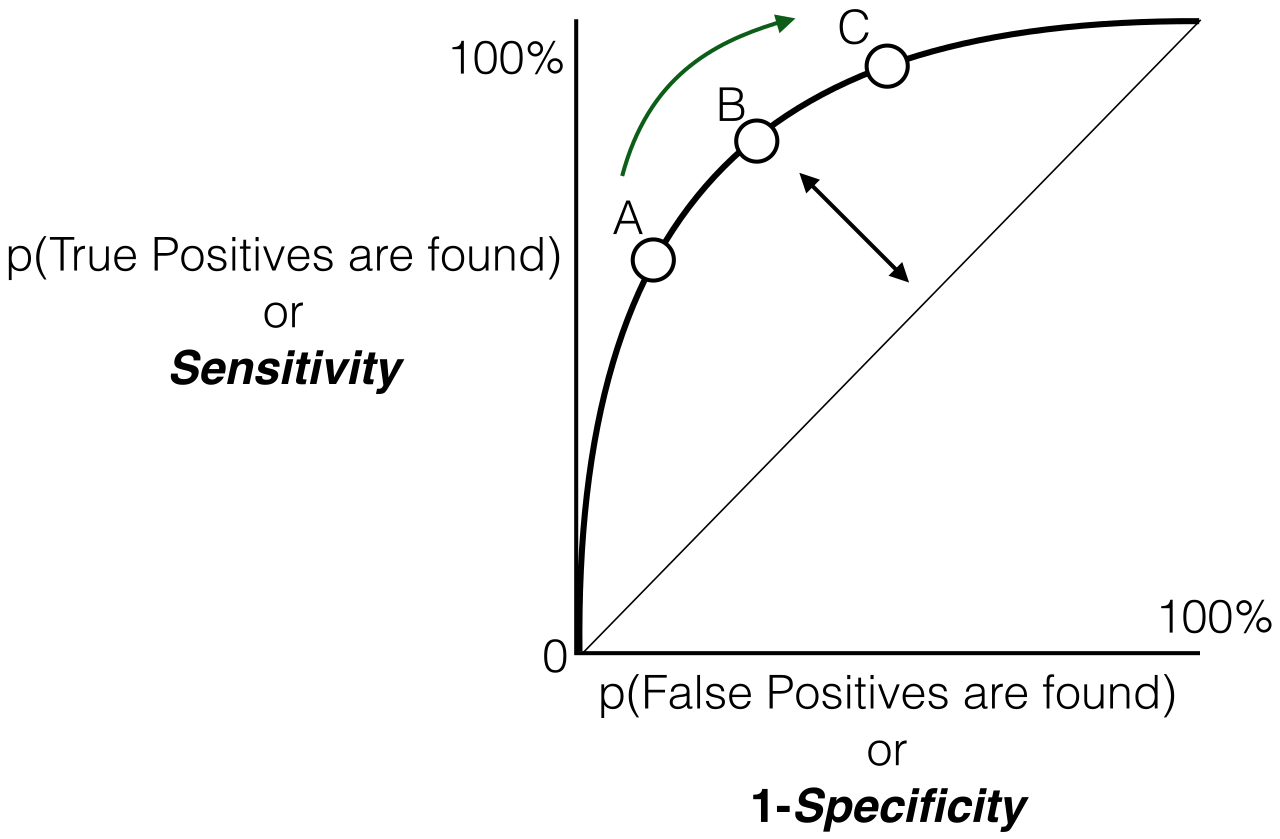
\includegraphics[width=0.76\linewidth]{assets/images/zobecnene-linearni-modely/roc-curve.png}
  \caption[ROC křivka]{ROC křivka pro binární klasifikaci. Popis obrázku: osa $y$ zobrazuje citlivost
  neboli true positive rate, osa $x$ falešně pozitivní míru neboli $1-\text{specificity}$. Body na křivce
  odpovídají různým rozhodovacím prahům; křivka blíže levému hornímu rohu znamená lepší diskriminaci.
  Zdroj obrázku: Masato8686819,
  \href{https://commons.wikimedia.org/wiki/File:ROC\_curve.svg}{Wikimedia Commons},
  licence CC BY-SA 3.0.}
  \label{fig:roc-curve}
\end{figure}

\subsection{Ordinální závisle proměnná}

Ordinální proměnná má více kategorií, které mají přirozené pořadí.

Příklady:
\begin{itemize}
    \item dosažené vzdělání: základní, střední, vysoké,
    \item spokojenost: nespokojen, neutrální, spokojen,
    \item odpověď v dotazníku: rozhodně ne, spíše ne, spíše ano, rozhodně ano.
\end{itemize}

Modelujeme latentní proměnnou:
\[
y_i^*=x_i^\top\beta+u_i.
\]

Pozorované kategorie vznikají podle prahů:
\[
y_i=k
\iff
\alpha_{k-1}<y_i^*\leq \alpha_k.
\]

Pravděpodobnost kategorie:
\[
P(y_i=k|x_i)
=
F(\alpha_k-x_i^\top\beta)
-
F(\alpha_{k-1}-x_i^\top\beta).
\]

Pokud je $F$ logistická distribuční funkce, jde o ordinální logit. Pokud je $F$ normální distribuční funkce,
jde o ordinální probit.

\paragraph{Intuice.}
Vyšší hodnota latentní proměnné posouvá pozorování do vyšších kategorií.

\subsection{Multinomická závisle proměnná}

Multinomická proměnná má více kategorií bez přirozeného pořadí:
\[
y_i\in\{0,1,\ldots,J\}.
\]

Příklady:
\begin{itemize}
    \item volba politické strany,
    \item volba dopravního prostředku,
    \item volba značky produktu,
    \item volba studijního oboru.
\end{itemize}

Protože kategorie nejsou uspořádané, nemůžeme použít ordinální logit/probit.

\subsection{Latentní užitek}

U multinomických modelů se často používá interpretace přes latentní užitek:
\[
U_{ij}=x_i^\top\beta_j+u_{ij}.
\]

Jedinec $i$ si vybere alternativu s nejvyšším užitkem:
\[
y_i=j
\iff
U_{ij}>U_{ih}
\quad
\text{pro všechna } h\neq j.
\]

\paragraph{Intuice.}
Při volbě mezi autem, autobusem a vlakem má každá alternativa pro člověka určitý užitek. Vybere tu, která
má nejvyšší užitek.

\subsection{Multinomický logit}

Pravděpodobnost volby alternativy $j$:
\[
P(y_i=j|x_i)
=
\frac{\exp(x_i^\top\beta_j)}
{\sum_{h=0}^{J}\exp(x_i^\top\beta_h)}.
\]

Protože pravděpodobnosti se musí sečíst na 1 a model jinak není identifikovaný, jedna kategorie se volí
jako referenční:
\[
\beta_0=0.
\]

Potom:
\[
\log\left(
\frac{P(y_i=j|x_i)}
{P(y_i=0|x_i)}
\right)
=
x_i^\top\beta_j.
\]

\paragraph{Interpretace.}
Koeficienty se interpretují vzhledem k referenční kategorii. Pokud je referenční volba například autobus,
pak koeficient u auta říká, jak proměnná mění log-poměr pravděpodobnosti volby auta proti autobusu.

Po exponenciaci:
\[
e^{\beta_{jr}}
\]
dostáváme relative risk ratio pro kategorii $j$ vůči referenční kategorii.

\subsection{IIA předpoklad}

Multinomický logit má důležitý předpoklad:
\[
IIA = \text{independence of irrelevant alternatives}.
\]

Tento předpoklad říká, že poměr pravděpodobností dvou alternativ nezávisí na dalších dostupných
alternativách:
\[
\frac{P(y=j|x)}{P(y=k|x)}
\]
se nezmění přidáním nebo odebráním jiné alternativy.

\paragraph{Problém.}
Pokud jsou některé alternativy blízké substituty, IIA může být nerealistický. Například přidání druhého
velmi podobného autobusu by nemělo stejně ovlivnit poměr volby auta a původního autobusu jako přidání
zcela jiné alternativy.

\subsection{Multinomický probit}

Multinomický probit umožňuje korelaci mezi chybami jednotlivých alternativ. Díky tomu nevyžaduje IIA.

Výhody:
\begin{itemize}
    \item flexibilnější,
    \item realističtější u podobných alternativ.
\end{itemize}

Nevýhody:
\begin{itemize}
    \item výpočetně náročný,
    \item horší použitelnost při velkém počtu kategorií.
\end{itemize}

\subsection{Čítací závisle proměnná}

Čítací proměnná nabývá hodnot:
\[
y_i\in\{0,1,2,\ldots\}.
\]

Příklady:
\begin{itemize}
    \item počet návštěv lékaře za rok,
    \item počet absencí v práci,
    \item počet nehod v regionu,
    \item počet nákupů zákazníka,
    \item počet defektů ve výrobní dávce.
\end{itemize}

Použít klasickou lineární regresi může být nevhodné, protože:
\begin{itemize}
    \item může predikovat záporné počty,
    \item počty bývají nesymetrické,
    \item rozptyl často roste se střední hodnotou.
\end{itemize}

\subsection{Poissonův regresní model}

Základní model:
\[
Y_i|x_i \sim Poisson(\mu_i).
\]

Poissonovo rozdělení:
\[
P(Y_i=y_i|x_i)
=
\frac{e^{-\mu_i}\mu_i^{y_i}}{y_i!}.
\]

Podmíněná střední hodnota:
\[
\mathrm{E}(Y_i|x_i)=\mu_i.
\]

Poissonův model používá log link:
\[
\log(\mu_i)=x_i^\top\beta.
\]

Tedy:
\[
\mu_i=\exp(x_i^\top\beta).
\]

\paragraph{Proč log link?}
Exponenciální funkce je vždy kladná, takže model nikdy nepredikuje záporný očekávaný počet.

\begin{figure}[htbp]
  \centering
  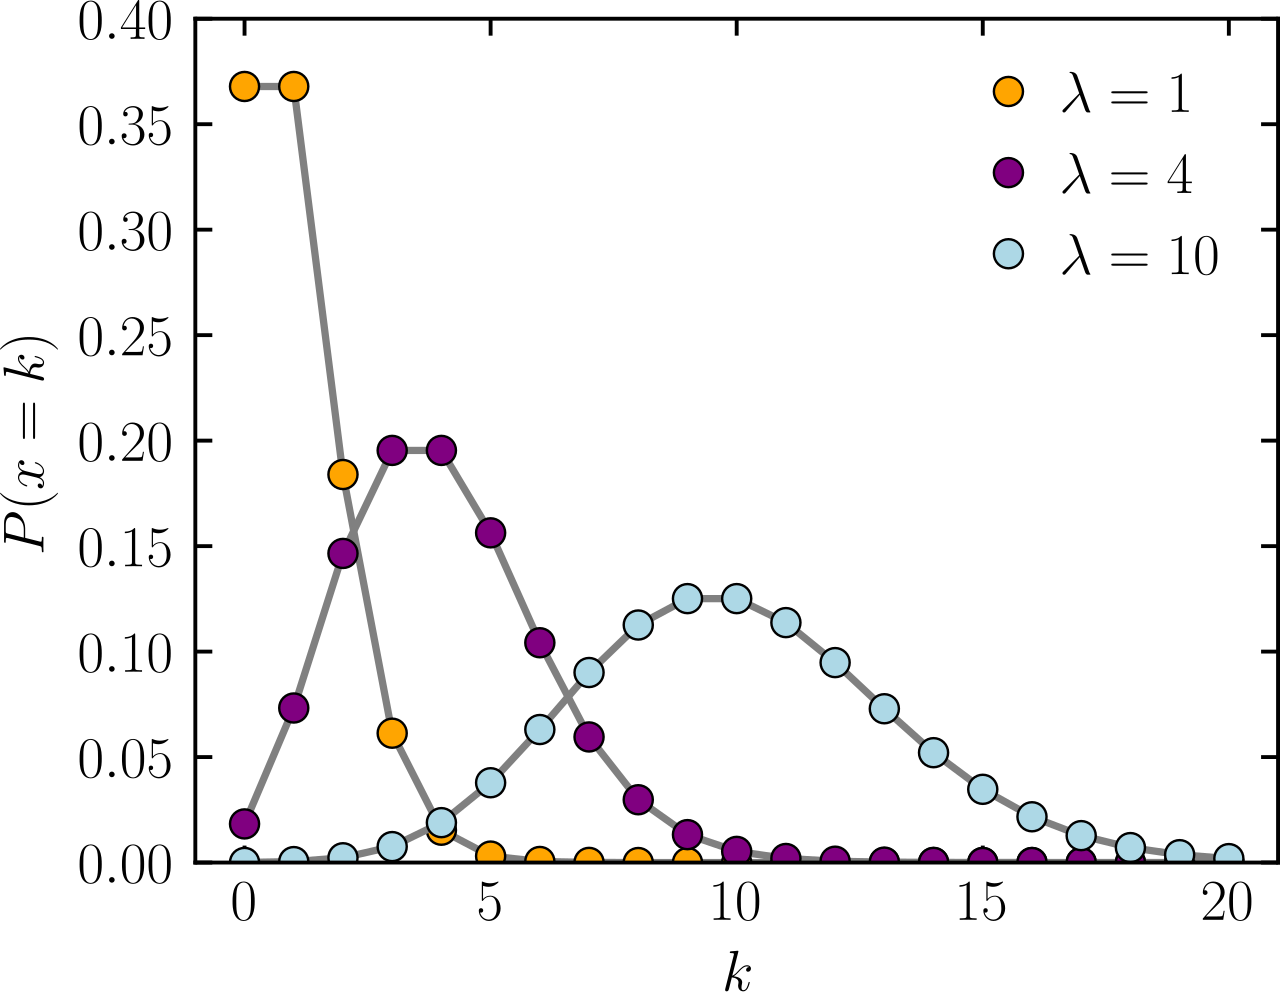
\includegraphics[width=0.76\linewidth]{assets/images/zobecnene-linearni-modely/poisson-pmf.png}
  \caption[Poissonovo rozdělení]{Pravděpodobnostní funkce Poissonova rozdělení pro různé hodnoty
  parametru $\lambda$. Popis obrázku: rozdělení je diskrétní, nabývá nezáporných celých hodnot a s rostoucí
  střední hodnotou se posouvá doprava. Právě proto se hodí pro modelování počtů událostí. Zdroj obrázku:
  Skbkekas, \href{https://commons.wikimedia.org/wiki/File:Poisson\_pmf.svg}{Wikimedia Commons},
  licence CC BY 3.0.}
  \label{fig:poisson-pmf}
\end{figure}

\subsection{Interpretace Poissonova modelu}

Protože:
\[
\mu_i=\exp(x_i^\top\beta),
\]
jednotková změna $x_j$ násobí očekávaný počet faktorem:
\[
e^{\beta_j}.
\]

Tento faktor se nazývá incidence rate ratio.

Procentní změna očekávaného počtu:
\[
100(e^{\beta_j}-1)\%.
\]

\paragraph{Příklad.}
Pokud:
\[
\beta_j=0.2,
\]
pak:
\[
e^{0.2}\approx 1.22.
\]
Jednotkové zvýšení $x_j$ zvyšuje očekávaný počet přibližně o 22\%.

\subsection{Marginální efekt v Poissonově modelu}

\[
\frac{\partial \mu_i}{\partial x_{ij}}
=
\beta_j\mu_i.
\]

To znamená, že absolutní změna očekávaného počtu závisí na aktuální úrovni $\mu_i$.

\paragraph{Intuice.}
Stejná procentní změna může znamenat malý absolutní rozdíl u jednotky s malým očekávaným počtem a velký
absolutní rozdíl u jednotky s vysokým očekávaným počtem.

\subsection{Offset a expozice}

Pokud mají jednotky různě dlouhou dobu sledování nebo různou velikost, je potřeba zahrnout expozici.

Například počet nehod závisí na délce sledovaného období nebo velikosti regionu.

Model:
\[
\log(\mu_i)=\log(t_i)+x_i^\top\beta.
\]

Kde:
\[
t_i
\]
je expozice.

Člen:
\[
\log(t_i)
\]
se nazývá offset.

\paragraph{Intuice.}
Pokud sledujeme jeden region dvakrát déle než jiný, očekáváme více událostí už jen kvůli delší expozici.
Offset to v modelu zohlední.

\subsection{Overdispersion}

Poissonův model předpokládá:
\[
\mathrm{E}(Y_i|x_i)=\mathrm{Var}(Y_i|x_i)=\mu_i.
\]

V praxi často platí:
\[
\mathrm{Var}(Y_i|x_i)>\mathrm{E}(Y_i|x_i).
\]

Tomu se říká overdispersion.

\paragraph{Důsledek.}
Pokud ignorujeme overdispersion, koeficienty mohou být rozumné, ale standardní chyby bývají příliš malé.
Proměnné pak mohou vypadat statisticky významněji, než skutečně jsou.

Možná řešení:
\begin{itemize}
    \item robustní standardní chyby,
    \item quasi-Poisson,
    \item negativně binomický model.
\end{itemize}

\subsection{Negativně binomický model}

Negativně binomický model umožňuje větší rozptyl:
\[
\mathrm{Var}(Y_i|x_i)=\mu_i+\alpha\mu_i^2,
\]
kde:
\[
\alpha>0.
\]

Pokud je $\alpha=0$, model se blíží Poissonovu modelu.

\paragraph{Intuice.}
Negativně binomický model je vhodný, pokud jsou v datech nepozorované rozdíly mezi jednotkami, které
zvyšují variabilitu počtů.

\subsection{Přebytek nul}

Někdy data obsahují více nul, než by odpovídalo Poissonovu nebo negativně binomickému modelu.

Příklady:
\begin{itemize}
    \item počet návštěv lékaře: mnoho lidí nemá žádnou návštěvu,
    \item počet nákupů: mnoho zákazníků nic nekoupí,
    \item počet nehod: mnoho regionů má nula nehod.
\end{itemize}

V takových případech lze použít:
\begin{itemize}
    \item zero-inflated modely,
    \item hurdle modely.
\end{itemize}

\subsubsection{Zero-inflated Poisson}

Zero-inflated model předpokládá dva procesy:
\begin{itemize}
    \item proces, který generuje strukturální nuly,
    \item běžný count proces.
\end{itemize}

Pravděpodobnost nuly:
\[
P(Y_i=0)
=
\pi_i+(1-\pi_i)e^{-\mu_i}.
\]

Pravděpodobnost kladného počtu:
\[
P(Y_i=y_i>0)
=
(1-\pi_i)
\frac{e^{-\mu_i}\mu_i^{y_i}}{y_i!}.
\]

\paragraph{Intuice.}
Některé jednotky mají nulu proto, že vůbec nemohou událost generovat. Jiné mají nulu jen náhodou v rámci
Poissonova procesu.

\subsubsection{Hurdle model}

Hurdle model má dvě části:
\begin{itemize}
    \item model, zda je hodnota nula nebo kladná,
    \item model kladných hodnot.
\end{itemize}

Nejdříve se tedy řeší, zda jednotka „překročí práh“ z nuly do kladného počtu, a potom se modeluje velikost
kladného počtu.

\subsection{Tobit model}

Tobit se používá pro omezenou závisle proměnnou, typicky pokud je mnoho hodnot na hranici, například nula.

Latentní model:
\[
y_i^*=x_i^\top\beta+u_i,
\]
kde:
\[
u_i|x_i\sim N(0,\sigma^2).
\]

Pozorovaná proměnná:
\[
y_i=\max(0,y_i^*).
\]

\paragraph{Příklady.}
\begin{itemize}
    \item výdaje na charitu, kde mnoho domácností dává 0,
    \item pracovní hodiny, pokud mnoho osob nepracuje,
    \item výdaje na určitý typ zboží, kde mnoho domácností nic nekoupí.
\end{itemize}

\paragraph{Rozdíl proti Poissonovi.}
Poisson je pro počty. Tobit je pro spojité hodnoty omezené zdola nebo shora.

\paragraph{Rozdíl proti cenzorování.}
U cenzorovaných dat skutečnou hodnotu neznáme přesně, protože je oříznutá. U corner solution je nula skutečná
hodnota, která má ekonomický význam.

\subsection{Diagnostika a praktické použití}

U nelineárních modelů nestačí sledovat jen znaménka a $p$-hodnoty koeficientů. Důležité je ověřit, zda
zvolený typ modelu odpovídá povaze závislé proměnné a účelu analýzy.

Typické kontroly:
\begin{itemize}
    \item \textbf{binární modely} -- klasifikační tabulka, ROC/AUC, citlivost, specificita, kalibrace
    pravděpodobností a vhodnost rozhodovacího prahu;
    \item \textbf{logit/probit} -- reportovat marginální efekty nebo predikované pravděpodobnosti, ne jen
    samotné koeficienty;
    \item \textbf{multinomický logit} -- promyslet, zda je realistický předpoklad IIA; při blízkých
    substitutech zvážit jiné modely nebo jiné členění kategorií;
    \item \textbf{Poissonův model} -- kontrolovat overdispersion, přebytek nul a správné použití
    expozice/offsetu;
    \item \textbf{inference} -- podle dat používat robustní nebo klastrované standardní chyby, zejména
    při heterogenitě jednotek nebo opakovaných pozorováních.
\end{itemize}

U logitu může nastat také perfektní nebo téměř perfektní separace: kombinace vysvětlujících proměnných
dokonale oddělí nuly a jedničky. V takové situaci maximum likelihood nemusí dát stabilní konečný odhad.

\subsection{Srovnání modelů podle typu závislé proměnné}

\begin{itemize}
    \item Spojitá přibližně normální proměnná:
    \[
    \text{lineární regrese}.
    \]
    
    \item Binární proměnná:
    \[
    \text{LPM, logit, probit}.
    \]
    
    \item Ordinální kategorie:
    \[
    \text{ordinální logit/probit}.
    \]
    
    \item Neuspořádané kategorie:
    \[
    \text{multinomický logit/probit}.
    \]
    
    \item Čítací proměnná:
    \[
    \text{Poisson, negativně binomický model}.
    \]
    
    \item Spojitá omezená proměnná s mnoha nulami:
    \[
    \text{Tobit}.
    \]
\end{itemize}

\subsection{Pozor u zkoušky}

Koeficient v logitu není změna pravděpodobnosti. Je to změna log-odds; pro pravděpodobnost je potřeba
uvést marginální efekt nebo konkrétní predikované pravděpodobnosti. Odds ratio také není totéž co změna
pravděpodobnosti o procentní body.

LPM není \uv{zakázaný} model, ale má omezení: může predikovat mimo interval $[0,1]$ a má
heteroskedasticitu. Pokud se použije, je potřeba aspoň robustní inference a opatrná interpretace.

U Poissonova modelu se koeficienty interpretují multiplikativně přes $e^{\beta_j}$ a modelují očekávaný
počet nebo míru. Offset není běžná vysvětlující proměnná s odhadovaným koeficientem, ale známá expozice,
která vstupuje s koeficientem 1.

Multinomický logit je citlivý na předpoklad IIA. Tobit je model pro spojitou omezenou proměnnou, ne pro
čítací data; Poisson je naopak pro nezáporné celé počty.

\subsection{Shrnutí ke zkoušce}

Zobecněné lineární modely a modely s omezenou závisle proměnnou používáme tehdy, když klasická lineární
regrese není vhodná kvůli povaze $y$.

Pro binární $y$ modelujeme:
\[
P(y=1|x).
\]
LPM je jednoduchý, ale může predikovat pravděpodobnosti mimo $[0,1]$ a má heteroskedasticitu. Logit a probit
řeší tento problém pomocí nelineární funkce:
\[
P(y=1|x)=F(x^\top\beta).
\]

U logitu koeficienty interpretujeme přes odds ratio:
\[
e^{\beta_j}.
\]
Pro změnu pravděpodobnosti používáme marginální efekty.

Pro neuspořádané kategorie používáme multinomický logit/probit. Multinomický logit je jednodušší, ale má
předpoklad IIA. Multinomický probit je flexibilnější, ale výpočetně náročnější.

Pro čítací data používáme Poissonův model:
\[
\log(\mu_i)=x_i^\top\beta.
\]
Koeficienty interpretujeme přes:
\[
e^{\beta_j},
\]
tedy jako násobení očekávaného počtu. Pokud je v datech overdispersion, používá se negativně binomický
model nebo robustní standardní chyby. Pokud je příliš mnoho nul, používají se zero-inflated nebo hurdle
modely.

\subsection{Zdroje}
\begin{itemize}
    \item statsmodels User Guide:
    \href{https://www.statsmodels.org/stable/glm.html}{Generalized Linear Models}.
    \item statsmodels User Guide:
    \href{https://www.statsmodels.org/stable/discretemod.html}{Regression with Discrete Dependent Variable}.
    \item scikit-learn User Guide:
    \href{https://scikit-learn.org/stable/modules/model\_evaluation.html\#roc-metrics}{Receiver operating characteristic}.
    \item Wikimedia Commons:
    \href{https://commons.wikimedia.org/wiki/File:Logistic-curve.svg}{File:Logistic-curve.svg}.
    \item Wikimedia Commons:
    \href{https://commons.wikimedia.org/wiki/File:ROC\_curve.svg}{File:ROC\_curve.svg}.
    \item Wikimedia Commons:
    \href{https://commons.wikimedia.org/wiki/File:Poisson\_pmf.svg}{File:Poisson\_pmf.svg}.
\end{itemize}



\newpage

\section{Ekonometrické modely pro časové řady a panelová data}

\subsection*{Základní rámec}

Ekonometrické modely pro \textbf{časové řady} a \textbf{panelová data} rozšiřují klasickou regresi o situace,
kdy pozorování nejsou jednoduše nezávislá. U časových řad záleží na pořadí pozorování v čase,
protože minulost často ovlivňuje současnost. U panelových dat sledujeme stejné jednotky opakovaně
v čase, a proto můžeme kontrolovat nepozorované vlastnosti jednotek, které se v čase nemění.

\begin{itemize}
    \item \textbf{Časová řada:} jedna proměnná nebo více proměnných pozorovaných v čase.
    \[
        y=\{y_t,\ t\in T\}.
    \]
    Typicky řešíme trend, sezónnost, autokorelaci, nestacionaritu a predikci.

    \item \textbf{Panelová data:} stejné jednotky $i=1,\dots,N$ pozorované v čase $t=1,\dots,T$.
    \[
        y_{it}, \qquad i=1,\dots,N,\quad t=1,\dots,T.
    \]
    Typicky řešíme nepozorovanou heterogenitu jednotek, fixed effects, random effects a dynamické panely.
\end{itemize}

\subsection*{1. Časové řady}

\subsubsection*{1.1 Co je časová řada}

Časová řada je posloupnost hodnot pozorovaných v pravidelných časových intervalech, například denně,
měsíčně, kvartálně nebo ročně. Důležité je, že pozorování nelze libovolně přeházet. Hodnota HDP v roce
2024 logicky navazuje na hodnotu z roku 2023, cena akcie dnes souvisí s cenou včera a nezaměstnanost
v jednom měsíci souvisí s nezaměstnaností v předchozích měsících.

\[
    y_t,\qquad t=1,\dots,T.
\]

Hlavní cíle analýzy časových řad jsou:
\begin{itemize}
    \item \textbf{pochopení mechanismu} generujícího data,
    \item \textbf{predikce budoucích hodnot},
    \item \textbf{testování hypotéz} o dynamice procesu,
    \item \textbf{modelování vztahů mezi proměnnými v čase}.
\end{itemize}

Oproti průřezovým datům je problém v tom, že pozorování v čase často nejsou nezávislá:
\[
    y_t \text{ může záviset na } y_{t-1}, y_{t-2}, \dots
\]

\subsubsection*{1.2 Komponenty časové řady}

Časovou řadu si často představujeme jako kombinaci několika složek:
\[
    y_t = Tr_t + S_t + C_t + u_t,
\]
kde:
\begin{itemize}
    \item $Tr_t$ je trend,
    \item $S_t$ je sezónní složka,
    \item $C_t$ je cyklická složka,
    \item $u_t$ je náhodná složka.
\end{itemize}

V jednodušší podobě:
\[
    y_t = Tr_t + u_t.
\]

\paragraph{Trend}

Trend znamená dlouhodobý růst nebo pokles časové řady. Může být deterministický nebo stochastický.

\textbf{Lineární deterministický trend:}
\[
    y_t = \alpha + \beta t + u_t.
\]

\textbf{Kvadratický trend:}
\[
    y_t = \alpha + \beta t + \gamma t^2 + u_t.
\]

Pokud trend odhadneme, detrendovaná řada je:
\[
    \widetilde y_t = y_t - \widehat{Tr}_t.
\]

Intuice: pokud chceme zkoumat vztah dvou ekonomických proměnných, neměli bychom ho zaměňovat
za fakt, že obě proměnné pouze rostou v čase. Například počet televizních seriálů i nějaký společenský
ukazatel mohou růst současně, ale to samo o sobě neznamená ekonomickou souvislost.

\paragraph{Zdánlivá regrese}

U nestacionárních časových řad může vzniknout \textbf{spurious regression}, tedy zdánlivá regrese.
Regrese může mít vysoké $R^2$ a statisticky významné koeficienty, přestože mezi proměnnými není
skutečný vztah. Často je důvodem společný trend.

Typický příklad:
\[
    y_t = \alpha + \beta x_t + u_t,
\]
kde $y_t$ i $x_t$ mají trend. Model pak může zachycovat hlavně to, že obě řady rostou s časem.

Řešení:
\begin{itemize}
    \item zahrnout trend $t$ do modelu,
    \item použít detrendovaná data,
    \item diferencovat časovou řadu,
    \item testovat jednotkový kořen a kointegraci.
\end{itemize}

\paragraph{Sezónnost}

Sezónnost znamená pravidelně se opakující vzorec v rámci roku, týdne nebo jiného cyklu.
Například maloobchodní tržby bývají vyšší v prosinci, spotřeba elektřiny se liší mezi zimou a létem.

Sezónnost lze modelovat pomocí dummy proměnných:
\[
    y_t =
    \alpha+\beta t+\delta_2D_{2t}+\cdots+\delta_sD_{st}+u_t.
\]

Pokud máme například měsíční data, používáme typicky 11 dummy proměnných, protože jedna sezóna
slouží jako referenční kategorie. Použití všech 12 dummy proměnných spolu s konstantou by vedlo
k perfektní multikolinearitě.

\subsubsection*{1.3 Stacionarita}

Stacionarita je jedna z nejdůležitějších vlastností časových řad. Obecně znamená, že základní
pravděpodobnostní vlastnosti procesu se v čase nemění. Pro ekonometrické modelování je důležitá
hlavně \textbf{slabá stacionarita}.

Proces $\{y_t\}$ je slabě stacionární, pokud:
\[
    E(y_t)=\mu
\]
je konstantní pro všechna $t$,

\[
    Var(y_t)=\gamma(0)
\]
je konstantní a

\[
    Cov(y_t,y_{t-h})=\gamma(h)
\]
závisí pouze na délce zpoždění $h$, nikoliv na konkrétním čase $t$.

Jinými slovy:
\begin{itemize}
    \item řada nemá měnící se průměr,
    \item řada nemá měnící se varianci,
    \item vztah mezi současností a minulostí závisí pouze na vzdálenosti v čase.
\end{itemize}

\paragraph{Bílý šum}

Bílý šum je základní stavební kámen mnoha modelů časových řad:
\[
    e_t \sim WN(0,\sigma^2).
\]

Platí:
\[
    E(e_t)=0,
\]
\[
    Var(e_t)=\sigma^2,
\]
\[
    Cov(e_t,e_s)=0 \quad \text{pro } t\neq s.
\]

Bílý šum je tedy posloupnost náhodných chyb bez autokorelace.

\subsubsection*{1.4 Autokorelace, ACF a PACF}

Autokorelace znamená korelaci časové řady se svou vlastní minulostí.

Autokovariance:
\[
    \gamma(h)=Cov(y_t,y_{t-h}).
\]

Autokorelace:
\[
    \rho(h)=\frac{\gamma(h)}{\gamma(0)}.
\]

\paragraph{ACF}

ACF, tedy autocorrelation function, ukazuje korelaci mezi $y_t$ a $y_{t-h}$ pro různá zpoždění $h$.
Používá se k odhalení persistence, sezónnosti a nestacionarity.

U stacionární řady ACF obvykle rychle klesá k nule. U nestacionární řady ACF často klesá velmi pomalu.

\paragraph{PACF}

PACF, tedy partial autocorrelation function, měří vztah mezi $y_t$ a $y_{t-h}$ po očištění vlivu
mezilehlých zpoždění $y_{t-1},\dots,y_{t-h+1}$.

\paragraph{Použití ACF a PACF při volbě modelu}

\begin{center}
\begin{tabular}{|p{0.35\textwidth}|p{0.55\textwidth}|}
\hline
\textbf{Chování ACF/PACF} & \textbf{Typický model} \\
\hline
PACF se po určitém zpoždění utne, ACF postupně doznívá & AR($p$) \\
\hline
ACF se po určitém zpoždění utne, PACF postupně doznívá & MA($q$) \\
\hline
ACF i PACF postupně doznívají & ARMA($p,q$) \\
\hline
ACF klesá velmi pomalu & podezření na nestacionaritu nebo jednotkový kořen \\
\hline
\end{tabular}
\end{center}

V praxi se ACF/PACF používají společně s informačními kritérii, jako jsou AIC a BIC, a s kontrolou reziduí.

\subsubsection*{1.5 Základní lineární modely časových řad}

\paragraph{MA(q) model}

Moving average model řádu $q$:
\[
    y_t = \alpha + e_t+\theta_1e_{t-1}+\cdots+\theta_qe_{t-q}.
\]

Současná hodnota závisí na současném a minulých náhodných šocích.

\paragraph{AR(p) model}

Autoregresní model řádu $p$:
\[
    y_t = \alpha+\phi_1y_{t-1}+\cdots+\phi_py_{t-p}+e_t.
\]

Současná hodnota závisí na vlastních minulých hodnotách. Například AR(1):
\[
    y_t=\alpha+\phi y_{t-1}+e_t.
\]

AR(1) je stacionární, pokud:
\[
    |\phi|<1.
\]

Pokud $\phi$ leží blízko jedné, proces je velmi perzistentní. Pokud $\phi=1$, dostáváme jednotkový
kořen a proces je nestacionární.

\paragraph{ARMA(p,q) model}

ARMA model kombinuje autoregresní a moving average složku:
\[
    y_t =
    \alpha+
    \sum_{i=1}^{p}\phi_i y_{t-i}
    +
    \sum_{j=1}^{q}\theta_j e_{t-j}
    +e_t.
\]

Používá se pro stacionární časové řady. Pokud řada není stacionární, je nutné ji nejprve transformovat,
například diferencováním.

\paragraph{ARIMA(p,d,q) model}

ARIMA model je rozšířením ARMA modelu pro nestacionární řady, které se stanou stacionárními po
diferencování.

První diference:
\[
    \Delta y_t = y_t-y_{t-1}.
\]

Druhá diference:
\[
    \Delta^2 y_t = \Delta y_t-\Delta y_{t-1}.
\]

ARIMA model:
\[
    \Delta^d y_t =
    \alpha+
    \sum_{i=1}^{p}\phi_i \Delta^d y_{t-i}
    +
    \sum_{j=1}^{q}\theta_j e_{t-j}
    +e_t.
\]

Parametry:
\begin{itemize}
    \item $p$ = počet autoregresních zpoždění,
    \item $d$ = počet diferencování nutných ke stacionaritě,
    \item $q$ = počet zpožděných šoků.
\end{itemize}

Speciální případ:
\[
    y_t=y_{t-1}+e_t
\]
je random walk, tedy ARIMA$(0,1,0)$.

\paragraph{SARIMA}

Pokud má řada sezónnost, používá se SARIMA:
\[
    SARIMA(p,d,q)\times(P,D,Q)_s,
\]
kde:
\begin{itemize}
    \item $s$ je délka sezóny,
    \item $P,D,Q$ jsou sezónní analogie parametrů $p,d,q$.
\end{itemize}

Například pro měsíční data bývá:
\[
    s=12.
\]

\subsubsection*{1.6 Jednotkový kořen a ADF test}

Jednotkový kořen znamená, že časová řada je nestacionární a šoky mají trvalý efekt. Typickým příkladem
je random walk:
\[
    y_t=y_{t-1}+e_t.
\]

Základní AR(1) proces:
\[
    y_t=\alpha+\phi y_{t-1}+e_t.
\]

Odečteme $y_{t-1}$:
\[
    y_t-y_{t-1}=\alpha+(\phi-1)y_{t-1}+e_t.
\]

Tedy:
\[
    \Delta y_t=\alpha+\beta_1y_{t-1}+e_t,
\]
kde:
\[
    \beta_1=\phi-1.
\]

Dickey--Fullerův test testuje:
\[
    H_0:\beta_1=0
\]
řada má jednotkový kořen, tedy je nestacionární,

\[
    H_1:\beta_1<0
\]
řada je stacionární.

ADF test, tedy augmented Dickey--Fuller test, přidává zpožděné diference, aby odstranil autokorelaci:
\[
    \Delta y_t =
    \alpha+\beta_1 y_{t-1}+\beta_2t
    +\delta_1\Delta y_{t-1}
    +\cdots+
    \delta_p\Delta y_{t-p}
    +e_t.
\]

Varianty testu:
\begin{itemize}
    \item bez konstanty,
    \item s konstantou,
    \item s konstantou a trendem.
\end{itemize}

Volba varianty závisí na povaze dat. Pokud řada viditelně roste v čase, je vhodné uvažovat variantu
s trendem.

\subsubsection*{1.7 Regrese s časovými řadami a autokorelace chyb}

Základní regresní model pro časové řady:
\[
    y_t=\beta_0+\beta_1x_{t1}+\cdots+\beta_kx_{tk}+u_t.
\]

Maticově:
\[
    y=X\beta+u.
\]

OLS odhad:
\[
    \hat\beta=(X^\top X)^{-1}X^\top y.
\]

Pro časové řady jsou důležité zejména tyto předpoklady:
\begin{itemize}
    \item linearita v parametrech,
    \item žádná perfektní multikolinearita,
    \item striktní exogenita:
    \[
        E(u_t\mid X)=0,
    \]
    \item homoskedasticita:
    \[
        Var(u_t\mid X)=\sigma^2,
    \]
    \item žádná autokorelace chyb:
    \[
        Cor(u_t,u_s\mid X)=0,\qquad t\neq s.
    \]
\end{itemize}

Pokud jsou chyby autokorelované, například:
\[
    u_t=\rho u_{t-1}+e_t,
\]
pak při splnění exogenity může být OLS stále nestranný a konzistentní, ale:
\begin{itemize}
    \item není efektivní,
    \item není BLUE,
    \item běžné směrodatné chyby jsou špatně,
    \item t-testy a F-testy mohou vést k chybným závěrům.
\end{itemize}

\paragraph{Durbin--Watsonův test}

Testuje hlavně AR(1) autokorelaci reziduí:
\[
    DW=
    \frac{\sum_{t=2}^{T}(\hat u_t-\hat u_{t-1})^2}
    {\sum_{t=1}^{T}\hat u_t^2}
    \approx 2(1-\hat\rho).
\]

Interpretace:
\begin{itemize}
    \item $DW\approx 2$: žádná autokorelace,
    \item $DW<2$: pozitivní autokorelace,
    \item $DW>2$: negativní autokorelace.
\end{itemize}

\paragraph{Breusch--Godfreyův test}

Obecnější test autokorelace řádu $p$:
\[
    u_t=\rho_1u_{t-1}+\cdots+\rho_pu_{t-p}+e_t.
\]

Pomocná regrese typicky vysvětluje rezidua $\hat u_t$ pomocí původních regresorů a zpožděných reziduí.

\paragraph{Řešení autokorelace}

\begin{itemize}
    \item \textbf{HAC / Newey--West směrodatné chyby:} neopravují samotný model, ale opravují inferenci.
    \item \textbf{GLS/FGLS:} transformují model tak, aby chyby byly blíže nekorelovaným a homoskedastickým.
    \item \textbf{Cochrane--Orcutt:} používá odhad $\rho$ a transformuje model:
    \[
        \widetilde y_t=y_t-\hat\rho y_{t-1},
    \]
    \[
        \widetilde x_{tj}=x_{tj}-\hat\rho x_{t-1,j}.
    \]
\end{itemize}

\subsubsection*{1.8 Regresní modely se zpožděnými proměnnými}

V ekonomii často účinky nevznikají okamžitě. Například změna úrokové sazby může ovlivnit investice
až s několikaměsíčním zpožděním. Proto používáme modely se zpožděnými proměnnými.

\paragraph{Regrese s ARMA chybami}

Model:
\[
    y_t=\alpha+\beta x_t+u_t,
\]
kde chyba má vlastní dynamiku:
\[
    u_t=
    \sum_{i=1}^{p}\phi_i u_{t-i}
    +
    \sum_{j=1}^{q}\theta_j e_{t-j}
    +e_t.
\]

Tento model říká, že $x_t$ působí současně, ale nevysvětlená část modelu má časovou strukturu.

\paragraph{ARMAX model}

ARMA model s exogenní proměnnou:
\[
    y_t=
    \alpha+\beta x_t
    +
    \sum_{i=1}^{p}\phi_i y_{t-i}
    +
    \sum_{j=1}^{q}\theta_j e_{t-j}
    +e_t.
\]

Rozdíl proti regresi s ARMA chybami je v interpretaci. V ARMAX modelu může $x_t$ působit i nepřímo
přes zpožděné hodnoty $y_t$.

\paragraph{FDL model}

Finite distributed lag model:
\[
    y_t=\alpha+\sum_{j=0}^{q}\delta_j x_{t-j}+u_t.
\]

Koeficient:
\[
    \delta_0
\]
je okamžitý efekt změny $x_t$ na $y_t$.

Dlouhodobý efekt permanentní změny $x$:
\[
    \delta=\sum_{j=0}^{q}\delta_j.
\]

Příklad interpretace: pokud $x$ trvale vzroste o jednu jednotku, potom se po odeznění všech zpoždění
$y$ změní o součet všech $\delta_j$.

\paragraph{ADL model}

Autoregressive distributed lag model:
\[
    y_t=
    \alpha+
    \sum_{i=1}^{p}\rho_i y_{t-i}
    +
    \sum_{j=0}^{q}\delta_j x_{t-j}
    +u_t.
\]

Tento model kombinuje:
\begin{itemize}
    \item zpožděné hodnoty závislé proměnné,
    \item současné i zpožděné hodnoty vysvětlující proměnné.
\end{itemize}

Dlouhodobý multiplikátor v ADL modelu je:
\[
    \frac{\sum_{j=0}^{q}\delta_j}{1-\sum_{i=1}^{p}\rho_i},
\]
pokud je model stabilní.

\subsubsection*{1.9 Predikce a volba modelu}

U časových řad je predikce velmi častým cílem. Predikce může být:
\begin{itemize}
    \item \textbf{bodová}, tedy jedna odhadnutá hodnota,
    \item \textbf{intervalová}, tedy interval možných hodnot.
\end{itemize}

Pro $h$-krokovou predikci označujeme:
\[
    \widehat y_{T+h}.
\]

Při delším predikčním horizontu obvykle roste nejistota, proto se intervaly predikce rozšiřují.

Modely se často porovnávají pomocí:
\[
    AIC=-2\ell+2K,
\]
\[
    BIC=-2\ell+K\ln(T),
\]
kde $\ell$ je log-likelihood a $K$ počet parametrů.

Nižší AIC/BIC znamená lepší kompromis mezi přesností a složitostí modelu.

Pro vyhodnocení predikcí se používají například:
\[
    MAE=\frac{1}{n}\sum_{t=1}^{n}|y_t-\hat y_t|,
\]
\[
    RMSE=\sqrt{\frac{1}{n}\sum_{t=1}^{n}(y_t-\hat y_t)^2}.
\]

Důležité je rozlišovat:
\begin{itemize}
    \item \textbf{in-sample fit}: jak model sedí na datech, na kterých byl odhadnut,
    \item \textbf{out-of-sample predikci}: jak model predikuje nová data.
\end{itemize}

\subsection*{2. Vícerozměrné časové řady, VAR a kointegrace}

\subsubsection*{2.1 Vícerozměrné časové řady}

Pokud sledujeme více časových řad současně, používáme vektor:
\[
    \mathbf y_t=(y_{t1},\dots,y_{tM})^\top.
\]

Například:
\[
    \mathbf y_t =
    \begin{pmatrix}
    HDP_t\\
    inflace_t\\
    urokova\ sazba_t
    \end{pmatrix}.
\]

Vícerozměrné modely jsou důležité, protože ekonomické veličiny se často ovlivňují navzájem.
Například úrokové sazby ovlivňují inflaci, ale zároveň centrální banka reaguje na inflaci úrokovými sazbami.

\subsubsection*{2.2 VAR model}

VAR model, tedy vector autoregression, modeluje více endogenních proměnných najednou.
Každá proměnná je vysvětlována vlastními zpožděními i zpožděními ostatních proměnných.

VAR($p$):
\[
    \mathbf y_t
    =
    \boldsymbol\alpha
    +
    \Phi_1\mathbf y_{t-1}
    +\cdots+
    \Phi_p\mathbf y_{t-p}
    +
    \mathbf e_t.
\]

Pro dvě proměnné a jedno zpoždění:
\[
    y_{1t}=\alpha_1+\phi_{11}y_{1,t-1}+\phi_{12}y_{2,t-1}+e_{1t},
\]
\[
    y_{2t}=\alpha_2+\phi_{21}y_{1,t-1}+\phi_{22}y_{2,t-1}+e_{2t}.
\]

Výhoda VAR modelu:
\begin{itemize}
    \item nemusíme předem určit jednu závislou a jednu nezávislou proměnnou,
    \item všechny proměnné mohou být endogenní,
    \item model zachycuje dynamické vazby mezi proměnnými.
\end{itemize}

Nevýhoda:
\begin{itemize}
    \item rychle roste počet parametrů,
    \item interpretace může být složitá,
    \item model vyžaduje dostatek dat.
\end{itemize}

\paragraph{Redukovaná a strukturální forma}

Redukovaná forma VAR neobsahuje současné hodnoty ostatních endogenních proměnných na pravé straně.
Současné vztahy jsou schovány v korelaci chyb.

Strukturální VAR může mít podobu:
\[
    A_0\mathbf y_t
    =
    \mathbf a
    +
    A_1\mathbf y_{t-1}
    +\cdots+
    A_p\mathbf y_{t-p}
    +
    \boldsymbol\varepsilon_t.
\]

Strukturální forma ale vyžaduje identifikační omezení, protože současné vztahy mezi proměnnými
nelze odhadnout automaticky bez dodatečných předpokladů.

\paragraph{Impulse response function}

Impulse response function popisuje, jak celý systém reaguje na jednorázový šok v jedné proměnné.
Například můžeme zkoumat, jak šok v úrokové sazbě ovlivní inflaci v dalších obdobích.

\subsubsection*{2.3 Grangerova kauzalita}

Proměnná $x$ Grangerovsky způsobuje proměnnou $y$, pokud minulost $x$ pomáhá predikovat $y$
nad rámec minulosti samotné proměnné $y$.

Ve VAR modelu testujeme, zda jsou koeficienty u zpožděných hodnot $x$ v rovnici pro $y$ nulové:
\[
    H_0:\phi_1=\phi_2=\cdots=\phi_p=0.
\]

Pokud $H_0$ zamítneme, minulost $x$ zlepšuje predikci $y$.

Důležité: Grangerova kauzalita není kauzalita v experimentálním smyslu. Znamená predikční vztah,
nikoliv nutně skutečný příčinný efekt.

\subsubsection*{2.4 Integrace a kointegrace}

Řada je integrována řádu $d$, značíme:
\[
    y_t \sim I(d),
\]
pokud je nutné ji $d$-krát diferencovat, aby byla stacionární.

Příklady:
\[
    I(0) = \text{stacionární řada},
\]
\[
    I(1) = \text{řada stacionární po první diferenci}.
\]

Random walk:
\[
    y_t=y_{t-1}+e_t
\]
je typický příklad $I(1)$ procesu.

\paragraph{Kointegrace}

Předpokládejme, že $y_t$ a $x_t$ jsou obě $I(1)$.
Regrese:
\[
    y_t=\alpha+\beta x_t+u_t
\]
může být zdánlivá. Pokud ale reziduum:
\[
    u_t=y_t-\alpha-\beta x_t
\]
je stacionární, tedy $I(0)$, potom jsou $y_t$ a $x_t$ kointegrované.

Intuice: jednotlivé řady mohou dlouhodobě růst nebo bloudit, ale existuje mezi nimi dlouhodobý
rovnovážný vztah, od kterého se neodchylují trvale.

\subsubsection*{2.5 Error Correction Model}

Pokud jsou dvě řady kointegrované, lze použít ECM:
\[
    \Delta y_t =
    \mu+\gamma\Delta x_t
    +\delta(y_{t-1}-\alpha-\beta x_{t-1})
    +e_t.
\]

Interpretace:
\begin{itemize}
    \item $\gamma$ zachycuje krátkodobý efekt změny $x$,
    \item $\alpha+\beta x_{t-1}$ zachycuje dlouhodobou rovnováhu,
    \item výraz $(y_{t-1}-\alpha-\beta x_{t-1})$ je odchylka od rovnováhy,
    \item $\delta$ je rychlost návratu k rovnováze.
\end{itemize}

Obvykle očekáváme:
\[
    \delta<0.
\]

Pokud je $y_{t-1}$ nad dlouhodobou rovnováhou, záporné $\delta$ tlačí $\Delta y_t$ dolů.

\subsubsection*{2.6 VECM}

VECM je vícerozměrná verze ECM pro kointegrované proměnné:
\[
    \Delta\mathbf y_t
    =
    \Pi\mathbf y_{t-1}
    +
    \Gamma_1\Delta\mathbf y_{t-1}
    +\cdots+
    \Gamma_{p-1}\Delta\mathbf y_{t-p+1}
    +
    \mathbf e_t.
\]

Pokud:
\[
    0<rank(\Pi)<M,
\]
existuje kointegrace a můžeme psát:
\[
    \Pi=\gamma\beta^\top.
\]

Zde:
\begin{itemize}
    \item $\beta^\top \mathbf y_t$ jsou kointegrační vztahy,
    \item $\gamma$ zachycuje rychlosti přizpůsobení k rovnováze.
\end{itemize}

\paragraph{Volba mezi VAR a VECM}

\begin{center}
\begin{tabular}{|p{0.42\textwidth}|p{0.45\textwidth}|}
\hline
\textbf{Situace} & \textbf{Vhodný model} \\
\hline
Všechny proměnné jsou $I(0)$ & VAR v úrovních \\
\hline
Proměnné jsou $I(1)$ a nejsou kointegrované & VAR v diferencích \\
\hline
Proměnné jsou $I(1)$ a jsou kointegrované & VECM \\
\hline
Jedna závislá proměnná a vysvětlující proměnné se zpožděními & FDL, ADL, ARMAX nebo ECM \\
\hline
\end{tabular}
\end{center}

\subsection*{3. Panelová data}

\subsubsection*{3.1 Co jsou panelová data}

Panelová data kombinují průřezovou a časovou dimenzi. Sledujeme stejné jednotky v čase:
\[
    y_{it},\qquad i=1,\dots,N,\quad t=1,\dots,T.
\]

Příklady:
\begin{itemize}
    \item stejní lidé sledovaní několik let,
    \item firmy sledované po kvartálech,
    \item země EU sledované po letech,
    \item kraje sledované v čase.
\end{itemize}

Rozdíl mezi pooled daty a panelem:
\begin{itemize}
    \item \textbf{Pooled cross sections:} v různých letech sledujeme různé jednotky.
    \item \textbf{Panelová data:} v různých letech sledujeme stejné jednotky.
\end{itemize}

\subsubsection*{3.2 Typy panelů}

\begin{itemize}
    \item \textbf{Vyvážený panel:} každá jednotka má pozorování ve všech obdobích.
    \item \textbf{Nevyvážený panel:} některá pozorování chybí.
    \item \textbf{Krátký panel:} velké $N$, malé $T$.
    \item \textbf{Dlouhý panel:} malé $N$, velké $T$.
    \item \textbf{Velký panel:} velké $N$ i velké $T$.
\end{itemize}

U krátkých panelů se často používají FE, RE, FD a související metody. U dlouhých panelů se více
objevují problémy podobné časovým řadám, například stacionarita a autokorelace.

\subsubsection*{3.3 Základní panelový model}

Základní panelová regrese:
\[
    y_{it}
    =
    \alpha
    +
    \mathbf x_{it}^\top\beta
    +
    \mathbf z_i^\top\gamma
    +
    u_{it}.
\]

Kde:
\begin{itemize}
    \item $\mathbf x_{it}$ jsou proměnné měnící se v čase,
    \item $\mathbf z_i$ jsou časově neměnné charakteristiky jednotky,
    \item $u_{it}$ je chyba.
\end{itemize}

Často ale některé důležité časově neměnné vlastnosti nepozorujeme. Pak píšeme:
\[
    y_{it}
    =
    \alpha
    +
    \mathbf x_{it}^\top\beta
    +
    c_i
    +
    u_{it}.
\]

Zde:
\[
    c_i
\]
je nepozorovaná heterogenita jednotky.

Příklady $c_i$:
\begin{itemize}
    \item vrozené schopnosti člověka,
    \item firemní kultura,
    \item geografická poloha regionu,
    \item instituce nebo historické faktory země.
\end{itemize}

Hlavní výhoda panelových dat je, že dokážou kontrolovat časově neměnné nepozorované faktory.

\subsubsection*{3.4 Pooled OLS}

Pooled OLS ignoruje panelovou strukturu a odhaduje obyčejnou regresi:
\[
    y_{it}=\alpha+\mathbf x_{it}^\top\beta+v_{it},
\]
kde:
\[
    v_{it}=c_i+u_{it}.
\]

Pooled OLS je problematický, pokud:
\[
    Cor(c_i,\mathbf x_{it})\neq 0.
\]

Pak je $c_i$ vynechaná proměnná korelovaná s regresory a odhad $\hat\beta$ je vychýlený.

Pooled OLS může být použitelný, pokud:
\[
    Cor(c_i,\mathbf X_i)=0,
\]
ale v praxi je to často silný předpoklad.

\subsubsection*{3.5 LSDV}

LSDV, tedy least squares dummy variables, přidává dummy proměnné pro jednotky:
\[
    y_{it}
    =
    \alpha_1I\{i=1\}
    +
    \alpha_2I\{i=2\}
    +\cdots+
    \alpha_NI\{i=N\}
    +
    \mathbf x_{it}^\top\beta
    +
    u_{it}.
\]

Každá jednotka má vlastní intercept:
\[
    \alpha_i=\alpha+c_i.
\]

Výhoda:
\begin{itemize}
    \item explicitně kontroluje nepozorovanou heterogenitu jednotek.
\end{itemize}

Nevýhoda:
\begin{itemize}
    \item při velkém $N$ je mnoho dummy proměnných,
    \item nelze pohodlně odhadovat efekty časově neměnných proměnných.
\end{itemize}

LSDV a FE dávají stejné odhady koeficientů $\beta$.

\subsubsection*{3.6 First Difference estimator}

Model:
\[
    y_{it}
    =
    \alpha
    +
    \mathbf x_{it}^\top\beta
    +
    c_i
    +
    u_{it}.
\]

Pro období $t-1$:
\[
    y_{i,t-1}
    =
    \alpha
    +
    \mathbf x_{i,t-1}^\top\beta
    +
    c_i
    +
    u_{i,t-1}.
\]

Odečtením dostaneme:
\[
    y_{it}-y_{i,t-1}
    =
    (\mathbf x_{it}-\mathbf x_{i,t-1})^\top\beta
    +
    (u_{it}-u_{i,t-1}).
\]

Tedy:
\[
    \Delta y_{it}
    =
    \Delta \mathbf x_{it}^\top\beta
    +
    \Delta u_{it}.
\]

Výhoda:
\[
    c_i
\]
zmizí, protože je v čase konstantní.

Nevýhody:
\begin{itemize}
    \item ztratíme první období,
    \item časově neměnné proměnné nelze odhadnout,
    \item pokud je chyba silně autokorelovaná, může být FD méně vhodný.
\end{itemize}

FD je přirozený zejména pro panel s $T=2$.

\subsubsection*{3.7 Fixed Effects estimator}

FE používá tzv. within transformaci. Nejprve vezmeme průměr přes čas pro jednotku $i$:
\[
    \bar y_i
    =
    \alpha
    +
    \bar{\mathbf x}_i^\top\beta
    +
    c_i
    +
    \bar u_i.
\]

Poté odečteme průměr od původní rovnice:
\[
    y_{it}-\bar y_i
    =
    (\mathbf x_{it}-\bar{\mathbf x}_i)^\top\beta
    +
    (u_{it}-\bar u_i).
\]

Člen $c_i$ zmizí.

FE tedy využívá pouze změny uvnitř jednotky v čase. Neptá se, proč mají některé jednotky vyšší
hodnoty než jiné, ale ptá se, co se stane, když se u téže jednotky změní $x$.

Interpretace:
\[
    \beta_j
\]
říká, jak se změní $y$ při změně $x_j$ uvnitř stejné jednotky v čase, po kontrole všech časově
neměnných vlastností jednotky.

Příklad: Pokud zkoumáme vliv vzdělání na mzdu a používáme individuální FE, kontrolujeme všechny
časově neměnné vlastnosti člověka, například schopnosti nebo rodinné zázemí, pokud se v čase nemění.

Nevýhody FE:
\begin{itemize}
    \item nelze odhadnout efekt časově neměnných proměnných,
    \item využívá jen vnitřní variabilitu,
    \item pokud se proměnná v čase téměř nemění, její efekt se odhaduje nepřesně.
\end{itemize}

\subsubsection*{3.8 Between estimator}

Between estimator používá pouze rozdíly mezi jednotkami. Odhaduje regresi časových průměrů:
\[
    \bar y_i
    =
    \alpha
    +
    \bar{\mathbf x}_i^\top\beta
    +
    e_i.
\]

Nevyužívá změny v čase, pouze to, že některé jednotky mají v průměru vyšší $x$ a jiné nižší $x$.
Proto neumí dobře kontrolovat nepozorovanou heterogenitu korelovanou s regresory.

Obecně je méně důležitý než FE a RE, ale pomáhá pochopit rozdíl mezi:
\begin{itemize}
    \item within variabilitou,
    \item between variabilitou.
\end{itemize}

\subsubsection*{3.9 Random Effects estimator}

Random effects model opět vychází z:
\[
    y_{it}
    =
    \alpha
    +
    \mathbf x_{it}^\top\beta
    +
    c_i
    +
    u_{it}.
\]

Rozdíl proti FE je v předpokladu:
\[
    Cor(c_i,\mathbf X_i)=0.
\]

Tedy nepozorovaná heterogenita jednotky nesmí korelovat s vysvětlujícími proměnnými.

Pokud tento předpoklad platí, RE je efektivnější než FE, protože využívá:
\begin{itemize}
    \item variabilitu uvnitř jednotek,
    \item variabilitu mezi jednotkami.
\end{itemize}

Navíc RE umožňuje odhadovat efekty časově neměnných proměnných.

Složená chyba:
\[
    v_{it}=c_i+u_{it}.
\]

RE používá quasi-demeaning:
\[
    y_{it}-\lambda\bar y_i
    =
    \alpha(1-\lambda)
    +
    (\mathbf x_{it}-\lambda\bar{\mathbf x}_i)^\top\beta
    +
    v_{it}-\lambda\bar v_i.
\]

Kde:
\[
    \lambda
    =
    1
    -
    \sqrt{
    \frac{1}{1+T\frac{Var(c_i)}{Var(u_{it})}}
    }.
\]

Pokud:
\[
    \lambda=0,
\]
RE se podobá pooled OLS.

Pokud:
\[
    \lambda=1,
\]
RE se blíží FE transformaci.

\subsubsection*{3.10 Hausmanův test}

Hausmanův test porovnává FE a RE.

Hypotéza:
\[
    H_0: Cor(c_i,\mathbf X_i)=0.
\]

Pokud platí $H_0$, RE je konzistentní a efektivnější než FE.
Pokud $H_0$ neplatí, RE je nekonzistentní a měli bychom preferovat FE.

Testová statistika:
\[
    H
    =
    (\hat\beta_{FE}-\hat\beta_{RE})^\top
    \left[
    Var(\hat\beta_{FE})-Var(\hat\beta_{RE})
    \right]^{-1}
    (\hat\beta_{FE}-\hat\beta_{RE}).
\]

Rozhodnutí:
\begin{itemize}
    \item nezamítneme $H_0$: RE je přijatelný,
    \item zamítneme $H_0$: preferujeme FE.
\end{itemize}

Praktická intuice:
\begin{itemize}
    \item FE je bezpečnější, pokud se bojíme korelace mezi $c_i$ a regresory,
    \item RE je efektivnější, ale stojí na silnějším předpokladu.
\end{itemize}

\subsubsection*{3.11 Correlated Random Effects}

CRE, tedy correlated random effects nebo Mundlakův přístup, dovoluje, aby nepozorovaná heterogenita
souvisela s průměry regresorů.

Model:
\[
    y_{it}
    =
    \alpha
    +
    \mathbf x_{it}^\top\beta
    +
    \bar{\mathbf x}_i^\top\theta
    +
    a_i
    +
    u_{it}.
\]

Zde:
\[
    \bar{\mathbf x}_i
\]
jsou časové průměry regresorů pro jednotku $i$.

Pokud jsou koeficienty $\theta$ významné, naznačuje to, že běžný RE předpoklad je problematický.
CRE je užitečný kompromis, protože umožňuje:
\begin{itemize}
    \item testovat korelaci mezi heterogenitou a regresory,
    \item interpretovat within i between efekty,
    \item někdy zachovat možnost odhadnout časově neměnné proměnné.
\end{itemize}

\subsubsection*{3.12 Časové efekty a two-way fixed effects}

Někdy existují šoky společné pro všechny jednotky v určitém čase. Například:
\begin{itemize}
    \item ekonomická krize,
    \item pandemie,
    \item změna regulace,
    \item technologická změna.
\end{itemize}

Model s časovými efekty:
\[
    y_{it}
    =
    \alpha
    +
    \mathbf x_{it}^\top\beta
    +
    c_i
    +
    d_t
    +
    u_{it}.
\]

Kde:
\[
    d_t
\]
je efekt společný pro všechny jednotky v čase $t$.

Pokud model obsahuje individuální efekty $c_i$ i časové efekty $d_t$, mluvíme o:
\[
    \text{two-way fixed effects}.
\]

Tento model kontroluje:
\begin{itemize}
    \item všechny časově neměnné rozdíly mezi jednotkami,
    \item všechny šoky společné pro jednotky v daném čase.
\end{itemize}

\subsubsection*{3.13 Robustní inference v panelech}

V panelových modelech často vzniká:
\begin{itemize}
    \item heteroskedasticita mezi jednotkami,
    \item autokorelace uvnitř jednotek,
    \item korelace mezi jednotkami ve stejném čase.
\end{itemize}

Proto se často používají robustní nebo clusterované směrodatné chyby.

\paragraph{Clusterování podle jednotek}

Umožňuje libovolnou korelaci chyb uvnitř jednotky v čase:
\[
    E(u_{it}u_{is})\neq 0.
\]

To je typické, pokud pozorování jedné firmy, osoby nebo země v čase spolu souvisí.

\paragraph{Clusterování podle času}

Umožňuje korelaci mezi jednotkami ve stejném období:
\[
    E(u_{it}u_{jt})\neq 0.
\]

To je důležité při společných makroekonomických šocích.

\paragraph{Two-way clustering}

Kombinuje clusterování podle jednotek i podle času.

Po odhadu panelového modelu je vhodné testovat autokorelaci reziduí, například:
\begin{itemize}
    \item Wooldridgeovým testem pro FE modely,
    \item Breusch--Godfreyho testem pro RE modely.
\end{itemize}

Pokud existuje korelace chyb, lze použít:
\begin{itemize}
    \item robustní/clusterované směrodatné chyby,
    \item FGLS,
    \item vhodnější specifikaci modelu.
\end{itemize}

\subsubsection*{3.14 Dynamické panelové modely}

Dynamický panel obsahuje zpožděnou závisle proměnnou:
\[
    y_{it}
    =
    \alpha
    +
    \rho y_{i,t-1}
    +
    \mathbf x_{it}^\top\beta
    +
    c_i
    +
    u_{it}.
\]

Tento model je vhodný, pokud má závislá proměnná setrvačnost. Například:
\begin{itemize}
    \item současná nezaměstnanost závisí na minulé nezaměstnanosti,
    \item současný zisk firmy závisí na minulém zisku,
    \item současná kriminalita závisí na minulé kriminalitě.
\end{itemize}

Problém: běžný FE odhad je v krátkých panelech vychýlený, protože zpožděná závislá proměnná
koreluje s transformovanou chybou. Tomu se říká dynamická panelová bias, často také Nickell bias.

\paragraph{Arellano--Bond estimator}

Začneme modelem:
\[
    y_{it}
    =
    \alpha
    +
    \rho y_{i,t-1}
    +
    \mathbf x_{it}^\top\beta
    +
    c_i
    +
    u_{it}.
\]

Nejprve diferencujeme, čímž odstraníme $c_i$:
\[
    \Delta y_{it}
    =
    \rho \Delta y_{i,t-1}
    +
    \Delta \mathbf x_{it}^\top\beta
    +
    \Delta u_{it}.
\]

Ale:
\[
    \Delta y_{i,t-1}=y_{i,t-1}-y_{i,t-2}
\]
je korelováno s:
\[
    \Delta u_{it}=u_{it}-u_{i,t-1}.
\]

Proto používáme instrumenty, typicky hlubší zpoždění:
\[
    y_{i,t-2},\ y_{i,t-3},\dots
\]

Odhad se provádí pomocí GMM.

Důležité diagnostiky:
\begin{itemize}
    \item test autokorelace v diferencovaných reziduích,
    \item u Arellano--Bond odhadu očekáváme AR(1) v diferencích,
    \item neměli bychom mít AR(2) v diferencích,
    \item používá se také Sarganův nebo Hansenův test instrumentů.
\end{itemize}

\subsection*{4. Shrnutí rozdílů mezi hlavními modely}

\begin{center}
\begin{tabular}{|p{0.36\textwidth}|p{0.54\textwidth}|}
\hline
\textbf{Situace} & \textbf{Vhodný přístup} \\
\hline
Jedna stacionární časová řada & AR, MA, ARMA \\
\hline
Nestacionární řada, která se po diferencování stane stacionární & ARIMA \\
\hline
Sezónní časová řada & Sezónní dummy nebo SARIMA \\
\hline
Regrese časových řad s autokorelací chyb & HAC SE, GLS/FGLS, ARMA chyby \\
\hline
Efekt proměnné se zpožděním & FDL, ADL, ARMAX \\
\hline
Více vzájemně propojených endogenních časových řad & VAR \\
\hline
Nestacionární, ale kointegrované řady & ECM nebo VECM \\
\hline
Panel s nepozorovanou heterogenitou korelovanou s regresory & FE nebo FD \\
\hline
Panel s heterogenitou nekorelovanou s regresory & RE \\
\hline
Volba mezi FE a RE & Hausmanův test a věcná argumentace \\
\hline
Panel s šoky společnými pro všechna období & časové efekty nebo two-way FE \\
\hline
Dynamický panel se zpožděným $y$ & Arellano--Bond / GMM \\
\hline
\end{tabular}
\end{center}

\subsection*{5. Nejdůležitější rovnice k zapamatování}

\[
    \text{AR(p):}\qquad
    y_t=\alpha+\sum_{i=1}^{p}\phi_i y_{t-i}+e_t.
\]

\[
    \text{ARMA(p,q):}\qquad
    y_t=
    \alpha+
    \sum_{i=1}^{p}\phi_i y_{t-i}
    +
    \sum_{j=1}^{q}\theta_j e_{t-j}
    +e_t.
\]

\[
    \text{ARIMA(p,d,q):}\qquad
    \Delta^d y_t=
    \alpha+
    \sum_{i=1}^{p}\phi_i\Delta^d y_{t-i}
    +
    \sum_{j=1}^{q}\theta_j e_{t-j}
    +e_t.
\]

\[
    \text{ADF test:}\qquad
    \Delta y_t =
    \alpha+\beta_1 y_{t-1}+\beta_2t
    +\delta_1\Delta y_{t-1}
    +\cdots+
    \delta_p\Delta y_{t-p}
    +e_t.
\]

\[
    \text{FDL:}\qquad
    y_t=\alpha+\sum_{j=0}^{q}\delta_jx_{t-j}+u_t.
\]

\[
    \text{ADL:}\qquad
    y_t=
    \alpha+
    \sum_{i=1}^{p}\rho_i y_{t-i}
    +
    \sum_{j=0}^{q}\delta_jx_{t-j}
    +u_t.
\]

\[
    \text{VAR(p):}\qquad
    \mathbf y_t
    =
    \boldsymbol\alpha
    +
    \sum_{i=1}^{p}\Phi_i\mathbf y_{t-i}
    +
    \mathbf e_t.
\]

\[
    \text{ECM:}\qquad
    \Delta y_t =
    \mu+\gamma\Delta x_t
    +\delta(y_{t-1}-\alpha-\beta x_{t-1})
    +e_t.
\]

\[
    \text{Panel FE:}\qquad
    y_{it}-\bar y_i
    =
    (\mathbf x_{it}-\bar{\mathbf x}_i)^\top\beta
    +
    (u_{it}-\bar u_i).
\]

\[
    \text{Panel FD:}\qquad
    \Delta y_{it}
    =
    \Delta \mathbf x_{it}^\top\beta
    +
    \Delta u_{it}.
\]

\[
    \text{Panel RE:}\qquad
    y_{it}-\lambda\bar y_i
    =
    \alpha(1-\lambda)
    +
    (\mathbf x_{it}-\lambda\bar{\mathbf x}_i)^\top\beta
    +
    v_{it}-\lambda\bar v_i.
\]

\[
    \text{Dynamický panel:}\qquad
    y_{it}
    =
    \alpha
    +
    \rho y_{i,t-1}
    +
    \mathbf x_{it}^\top\beta
    +
    c_i
    +
    u_{it}.
\]


\newpage

\section{Strojové učení. Druhy úloh strojového učení, klasifikace algoritmů, dostupné nástroje}


\subsection*{Vymezení strojového učení}

Strojové učení je oblast umělé inteligence, ve které se systém učí ze vzorových dat a na jejich základě
zlepšuje své rozhodování, predikce nebo rozpoznávání vzorů. Rozdíl proti klasickému programování je v tom,
že pravidla nejsou plně ručně naprogramována, ale jsou odhadnuta z dat.

Typicky máme:
\[
X = (x_1,\ldots,x_p)
\]
jako vstupní atributy, prediktory nebo features, a u učení s učitelem také cílovou proměnnou:
\[
y.
\]

Cílem modelu je naučit se funkci:
\[
\hat{f}: X \rightarrow y,
\]
která dobře funguje nejen na trénovacích datech, ale hlavně na nových datech.

\paragraph{Intuice.}
U klasického programování řekneme počítači přesná pravidla. U strojového učení mu dáme příklady a algoritmus
se pokusí pravidla najít sám. Například místo ruční definice, co je spam, model dostane mnoho označených
e-mailů a učí se, jaké vlastnosti se spamem souvisí.

\subsection*{Pattern recognition a data mining}

V materiálech se objevuje pojem \term{pattern recognition}, tedy rozpoznávání vzorů. Na vstupu jsou surová
data a na výstupu je akce, klasifikace nebo doporučení podle nalezených vzorů.

Příklady:
\begin{itemize}
    \item detekce podvodné platby,
    \item rozpoznávání řeči nebo obrazu,
    \item klasifikace zákazníků,
    \item predikce spotřeby elektřiny,
    \item analýza clickstreamů v e-shopu,
    \item text mining.
\end{itemize}

\term{Data mining} neboli dobývání znalostí z databází je proces hledání netriviálních, potenciálně
užitečných a srozumitelných vztahů v rozsáhlých datech. V praxi je silně propojen s datovými sklady,
datovou kvalitou, business znalostí a interpretací výsledků.

\subsection*{Základní druhy úloh strojového učení}

\subsubsection*{Učení s učitelem}

Učení s učitelem má k dispozici trénovací data:
\[
\{(x_i,y_i)\}_{i=1}^n.
\]

U každého objektu známe cílovou proměnnou $y_i$. Model se učí vztah mezi vstupy $x_i$ a výstupem $y_i$.

\paragraph{Klasifikace.}
Cílová proměnná je kategoriální:
\[
y_i \in \{1,\ldots,K\}.
\]

Příklady:
\begin{itemize}
    \item schválit / neschválit úvěr,
    \item spam / ne-spam,
    \item zákazník odejde / neodejde,
    \item diagnóza pacienta,
    \item segment zákazníka.
\end{itemize}

\paragraph{Regrese.}
Cílová proměnná je číselná:
\[
y_i \in \mathbb{R}.
\]

Příklady:
\begin{itemize}
    \item predikce ceny nemovitosti,
    \item predikce spotřeby energie,
    \item odhad tržeb,
    \item predikce pojistných nákladů.
\end{itemize}

\subsubsection*{Učení bez učitele}

Učení bez učitele nemá cílovou proměnnou. Máme pouze:
\[
\{x_i\}_{i=1}^n.
\]

Cílem je najít strukturu v datech.

Typické úlohy:
\begin{itemize}
    \item \term{shlukování} -- hledání skupin podobných objektů,
    \item \term{asociační pravidla} -- hledání souvislostí mezi položkami,
    \item \term{redukce dimenze} -- PCA, autoenkodéry,
    \item \term{detekce anomálií} -- hledání neobvyklých pozorování.
\end{itemize}

\paragraph{Příklad.}
U zákazníků neznáme předem segmenty. Shlukovací algoritmus se pokusí najít skupiny zákazníků podle podobného
chování, nákupů nebo demografie.

\subsubsection*{Doporučování}

Doporučovací systémy predikují, jaké položky by uživatele mohly zajímat. V materiálech se objevuje
\term{collaborative filtering}, například doporučování filmů podle matice uživatel--položka.

Typická vstupní matice:
\[
R =
\begin{pmatrix}
r_{11} & r_{12} & \cdots & r_{1m}\\
r_{21} & r_{22} & \cdots & r_{2m}\\
\vdots & \vdots & \ddots & \vdots\\
r_{n1} & r_{n2} & \cdots & r_{nm}
\end{pmatrix},
\]
kde $r_{ij}$ je hodnocení položky $j$ uživatelem $i$.

Jedna možnost je rozklad:
\[
R \approx U \Sigma V^\top,
\]
tedy singulární rozklad, který hledá latentní faktory uživatelů a položek.

\subsubsection*{Detekce anomálií}

Detekce anomálií hledá pozorování, která se výrazně liší od běžných dat. Může být:
\begin{itemize}
    \item supervised, pokud máme označené podvody/anomálie,
    \item unsupervised, pokud označení nemáme.
\end{itemize}

Příklad z praxe je detekce podvodných plateb. Pokud není k dispozici dostatek označených podvodů, lze použít
například \term{Isolation Forest}. Ten izoluje neobvyklé body pomocí náhodných stromů; anomálie bývají
izolovány menším počtem dělení.

\subsection*{Klasifikace algoritmů}

\subsubsection*{Podle typu úlohy}

\begin{itemize}
    \item \textbf{Klasifikační algoritmy:}
    rozhodovací stromy, logistická regrese, k-NN, Naive Bayes, SVM, random forest, boosting,
    neuronové sítě.
    
    \item \textbf{Regresní algoritmy:}
    lineární regrese, regresní stromy, random forest regressor, gradient boosting regressor,
    support vector regression, neuronové sítě.
    
    \item \textbf{Shlukovací algoritmy:}
    k-means, hierarchické shlukování, DBSCAN, aglomerativní metody.
    
    \item \textbf{Asociační pravidla:}
    Apriori, FP-Growth, GUHA, 4FT-Miner.
    
    \item \textbf{Redukce dimenze:}
    PCA, SVD, t-SNE, UMAP, autoenkodéry.
\end{itemize}

\subsubsection*{Podle interpretovatelnosti}

\begin{itemize}
    \item \textbf{White-box modely:}
    lineární/logistická regrese, malé rozhodovací stromy, pravidla, rozhodovací tabulky.
    
    \item \textbf{Black-box modely:}
    random forest, gradient boosting, SVM s nelineárním kernelem, neuronové sítě.
\end{itemize}

White-box model je srozumitelnější, ale nemusí mít nejlepší predikční výkon. Black-box model může být přesnější,
ale často vyžaduje dodatečné vysvětlovací metody, například LIME, SHAP nebo parciální závislosti.

\paragraph{No-Free-Lunch princip.}
Neexistuje jeden algoritmus, který by byl nejlepší pro všechny problémy. Algoritmus se vybírá podle cíle,
povahy dat, velikosti datasetu, požadavků na interpretaci, nákladů chyb a výpočetních omezení.

\subsection*{Vybrané algoritmy}

\subsubsection*{Rozhodovací strom}

Rozhodovací strom rozděluje data pomocí pravidel typu:
\[
x_j \leq c.
\]

Výsledkem je strom, jehož listy obsahují predikci třídy nebo hodnoty. Výhodou je vysoká interpretovatelnost.
Nevýhodou je sklon k přeučení.

\subsubsection*{k-nearest neighbours}

k-NN klasifikuje nový objekt podle nejbližších trénovacích objektů. Pro nový objekt $x$ najdeme $k$ nejbližších
sousedů a zvolíme nejčastější třídu:
\[
\hat{y}(x)=\operatorname{mode}\{y_i: x_i \in N_k(x)\}.
\]

Typická vzdálenost pro numerická data:
\[
d(x,z)=\sqrt{\sum_{j=1}^p (x_j-z_j)^2}.
\]

Výhody:
\begin{itemize}
    \item jednoduchý princip,
    \item žádný silný předpoklad o tvaru rozhodovací hranice,
    \item přirozená lokální interpretace přes podobné příklady.
\end{itemize}

Nevýhody:
\begin{itemize}
    \item citlivost na škálování proměnných,
    \item vysoká paměťová a výpočetní náročnost při predikci,
    \item curse of dimensionality: ve vysoké dimenzi se vzdálenosti stávají méně informativní.
\end{itemize}

\subsubsection*{Naive Bayes}

Naive Bayes vychází z Bayesovy věty:
\[
P(c|x)=\frac{P(x|c)P(c)}{P(x)}.
\]

Pro klasifikaci stačí maximalizovat čitatel:
\[
\hat{c}
=
\underset{c}{\operatorname{argmax}}
\,
P(c)P(x|c).
\]

Protože $x=(x_1,\ldots,x_p)$ může mít mnoho atributů, Naive Bayes zavádí zjednodušující předpoklad
podmíněné nezávislosti:
\[
P(x|c)=\prod_{j=1}^p P(x_j|c).
\]

Potom:
\[
\hat{c}
=
\underset{c}{\operatorname{argmax}}
\,
P(c)\prod_{j=1}^p P(x_j|c).
\]

Je „naivní“, protože atributy obvykle nezávislé nejsou. Přesto často funguje dobře, hlavně v textové
klasifikaci.

\paragraph{Laplace correction.}
Pokud se některá kombinace ve trénovacích datech nevyskytne, pravděpodobnost by byla nulová. Proto se používá
vyhlazení:
\[
\hat{P}(x_j=a|c)=
\frac{n_{a,c}+\alpha}{n_c+\alpha m},
\]
kde $m$ je počet možných hodnot atributu a $\alpha$ je obvykle 1.

\subsubsection*{SVM}

Support Vector Machine hledá nadrovinu, která odděluje třídy a maximalizuje margin:
\[
w^\top x + b = 0.
\]

U lineárně separovatelných dat:
\[
y_i(w^\top x_i+b)\geq 1.
\]

Optimalizační úloha hard-margin SVM:
\[
\min_{w,b}\frac{1}{2}\|w\|^2
\quad
\text{s.t.}
\quad
y_i(w^\top x_i+b)\geq 1.
\]

Šířka marginu je:
\[
\frac{2}{\|w\|}.
\]

U neseparovatelných dat se používá soft-margin SVM se slack proměnnými:
\[
\min_{w,b,\xi}
\frac{1}{2}\|w\|^2 + C\sum_{i=1}^n \xi_i
\]
\[
y_i(w^\top x_i+b)\geq 1-\xi_i,
\qquad
\xi_i\geq 0.
\]

Parametr $C$ řídí kompromis mezi širokým marginem a chybami klasifikace.

Pro nelineární data lze použít kernel:
\[
K(x_i,x_j).
\]

Příklady:
\[
K(x,z)=x^\top z
\quad \text{lineární kernel},
\]
\[
K(x,z)=(x^\top z+r)^d
\quad \text{polynomiální kernel},
\]
\[
K(x,z)=\exp(-\gamma\|x-z\|^2)
\quad \text{RBF kernel}.
\]

\subsubsection*{Neuronové sítě}

Neuronové sítě skládají mnoho jednoduchých výpočtových jednotek. U mělké sítě máme vstupní vrstvu, jednu
skrytou vrstvu a výstupní vrstvu. Detailněji jsou popsány v otázce 15.

\subsection*{CRISP-DM jako metodika analytického projektu}

CRISP-DM je standardní metodika pro data mining projekty. Má šest fází:

\begin{enumerate}
    \item \term{Business understanding}:
    pochopení problému, cíle, omezení, nákladů chyb a očekávaného využití.
    
    \item \term{Data understanding}:
    získání dat, pochopení atributů, kvality, rozsahu a omezení.
    
    \item \term{Data preparation}:
    čištění, spojování dat, imputace, odstranění duplicit, transformace, feature engineering.
    
    \item \term{Modeling}:
    volba algoritmů, trénování modelů, ladění hyperparametrů.
    
    \item \term{Evaluation}:
    ověření kvality modelu, kontrola, zda model řeší původní business problém.
    
    \item \term{Deployment}:
    nasazení modelu, reporting, API, automatizace, monitoring a údržba.
\end{enumerate}

V praxi bývá nejvíce práce v komunikaci s vlastníkem dat, čištění, přípravě dat, interpretaci a zajištění
důvěry ve výsledky, ne v samotném spuštění algoritmu.

\subsection*{Příprava dat}

Před modelováním je nutné řešit:

\begin{itemize}
    \item \textbf{Chybějící hodnoty:}
    odstranění řádků, imputace průměrem/mediánem, regresní imputace, modelová imputace.
    
    \item \textbf{Škálování:}
    důležité pro k-NN, SVM, neuronové sítě a clustering.
    
    \item \textbf{Kódování kategorií:}
    dummy proměnné, one-hot encoding, ordinal encoding.
    
    \item \textbf{Feature engineering:}
    tvorba nových atributů z doménové znalosti.
    
    \item \textbf{Feature selection:}
    výběr relevantních proměnných.
    
    \item \textbf{Data leakage:}
    nesmí se použít informace, která by v okamžiku predikce nebyla dostupná.
\end{itemize}

Standardizace:
\[
z_{ij}=\frac{x_{ij}-\bar{x}_j}{s_j}.
\]

Min-max škálování:
\[
x_{ij}^{*}=
\frac{x_{ij}-\min(x_j)}
{\max(x_j)-\min(x_j)}.
\]

\subsection*{Rozdělení dat a validace}

Dostupná označená data se obvykle rozdělí na:

\begin{itemize}
    \item \term{trénovací množinu} -- model se na ní učí,
    \item \term{validační množinu} -- ladění hyperparametrů a výběr modelu,
    \item \term{testovací množinu} -- finální nezávislé ověření kvality.
\end{itemize}

Jednoduché rozdělení:
\[
D = D_{\text{train}} \cup D_{\text{test}}.
\]

\subsubsection*{Křížová validace}

U $K$-fold cross-validation se data rozdělí na $K$ částí. Model se $K$krát natrénuje, vždy na $K-1$ částech,
a ověří na zbývající části.

Průměrná chyba:
\[
CV_K
=
\frac{1}{K}
\sum_{k=1}^K Err_k.
\]

\paragraph{Stratifikace.}
U nevyvážených tříd je vhodné zachovat podíly tříd v každém foldu.

\paragraph{Time-based split.}
U časově závislých dat se nesmí náhodně míchat minulost a budoucnost. Trénujeme na minulosti a testujeme
na pozdějších datech.

\subsection*{Hodnocení klasifikačních modelů}

Pro binární klasifikaci:

\[
\begin{array}{c|cc}
 & \text{Skutečně pozitivní} & \text{Skutečně negativní}\\
\hline
\text{Predikováno pozitivní} & TP & FP\\
\text{Predikováno negativní} & FN & TN
\end{array}
\]

\subsubsection*{Accuracy}

\[
Accuracy=
\frac{TP+TN}{TP+TN+FP+FN}.
\]

Accuracy může být zavádějící u nevyvážených tříd.

\subsubsection*{Precision}

\[
Precision=
\frac{TP}{TP+FP}.
\]

Říká, jaká část pozitivních predikcí byla skutečně pozitivní.

\subsubsection*{Recall / sensitivity}

\[
Recall=
\frac{TP}{TP+FN}.
\]

Říká, jaká část skutečně pozitivních případů byla nalezena.

\subsubsection*{Specificity}

\[
Specificity=
\frac{TN}{TN+FP}.
\]

Říká, jaká část skutečně negativních případů byla správně označena jako negativní.

\subsubsection*{F1 score}

\[
F_1=
2\cdot
\frac{Precision\cdot Recall}
{Precision+Recall}.
\]

F1 je vhodné, pokud chceme vyvážit precision a recall.

\subsubsection*{ROC a AUC}

ROC křivka zobrazuje vztah:
\[
TPR = \frac{TP}{TP+FN}
\]
proti:
\[
FPR = \frac{FP}{FP+TN}.
\]

AUC shrnuje ROC křivku do jednoho čísla:
\[
AUC=1
\]
znamená perfektní klasifikátor,
\[
AUC=0.5
\]
odpovídá náhodnému klasifikátoru.

\subsection*{Cost-sensitive evaluation}

Ne všechny chyby mají stejný náklad. Například v medicíně může být falešně negativní chyba mnohem
dražší než falešně pozitivní.

Celkový náklad:
\[
Cost
=
C_{TP}TP+C_{FP}FP+C_{FN}FN+C_{TN}TN.
\]

Klasifikační práh lze zvolit tak, aby minimalizoval náklad:
\[
t^*
=
\underset{t}{\operatorname{argmin}}
\,
Cost(t).
\]

\subsection*{Overfitting a underfitting}

\term{Underfitting} znamená, že model je příliš jednoduchý a špatně zachytí strukturu dat.
Má vysokou chybu na trénovacích i testovacích datech.

\term{Overfitting} znamená, že model se naučil i šum a náhodné zvláštnosti trénovací množiny.
Má nízkou chybu na trénovacích datech, ale vysokou chybu na testovacích datech.

\[
Err_{\text{train}} \ll Err_{\text{test}}
\quad \Rightarrow \quad
\text{podezření na overfitting}.
\]

Řešení:
\begin{itemize}
    \item jednodušší model,
    \item regularizace,
    \item pruning stromů,
    \item více dat,
    \item cross-validation,
    \item ensemble metody,
    \item správné ladění hyperparametrů.
\end{itemize}

\subsection*{Ladění hyperparametrů}

Parametry se učí z dat. Hyperparametry nastavujeme před učením.

Příklady:
\begin{itemize}
    \item počet sousedů $k$ u k-NN,
    \item hloubka stromu,
    \item počet stromů v random forest,
    \item learning rate u boostingu nebo neuronových sítí,
    \item parametr $C$ a kernel u SVM.
\end{itemize}

Metody ladění:
\begin{itemize}
    \item grid search,
    \item random search,
    \item cross-validation,
    \item nested cross-validation.
\end{itemize}

\subsection*{Dostupné nástroje}

\begin{itemize}
    \item \textbf{Python:}
    pandas, numpy, scikit-learn, matplotlib, seaborn, scipy, xgboost, lightgbm, tensorflow, pytorch.
    
    \item \textbf{R:}
    caret, tidymodels, randomForest, e1071, nnet, rpart.
    
    \item \textbf{GUI nástroje:}
    Weka, RapidMiner, KNIME, IBM SPSS Modeler, SAS Enterprise Miner.
    
    \item \textbf{Akademické a specializované nástroje:}
    LISp-Miner, GUHA, 4FT-Miner.
    
    \item \textbf{Cloud a produkční nástroje:}
    BigML, cloudové ML služby, kontejnery, API, CI/CD, monitoring modelů.
\end{itemize}

Materiály zmiňují práci v Pythonu a scikit-learn, cloudové nástroje, BigML pro stromy a LISp-Miner jako
systém navazující na GUHA.

\subsection*{Shrnutí otázky}

Strojové učení je přístup, kdy se model učí ze vzorových dat. Základní dělení je učení s učitelem,
učení bez učitele, doporučování a detekce anomálií. Učení s učitelem zahrnuje klasifikaci a regresi,
učení bez učitele shlukování, asociační pravidla a redukci dimenze.

Typický ML projekt se řídí logikou CRISP-DM: pochopení businessu, pochopení dat, příprava dat, modelování,
vyhodnocení a nasazení. Kvalita modelu se nehodnotí na trénovacích datech, ale na validačních/testovacích
datech pomocí vhodných metrik. Je nutné hlídat overfitting, data leakage, nevyvážené třídy a náklady chyb.

\newpage
\section{Shlukové a klasifikační úlohy strojového učení. Rozhodovací stromy, shlukovací algoritmy, asociační pravidla}


\subsection*{Klasifikační úloha}

Klasifikace je úloha učení s učitelem. Každý objekt je popsán vstupními atributy:
\[
x_i=(x_{i1},\ldots,x_{ip}),
\]
a má známou cílovou třídu:
\[
y_i\in\{1,\ldots,K\}.
\]

Cílem je naučit klasifikátor:
\[
\hat{f}(x_i)=\hat{y}_i,
\]
který dokáže přiřadit nová pozorování do správné třídy.

\paragraph{Příklady.}
\begin{itemize}
    \item zákazník odejde / neodejde,
    \item transakce je podvodná / nepodvodná,
    \item e-mail je spam / ne-spam,
    \item pacient má / nemá danou diagnózu,
    \item klient je dobrý / rizikový žadatel o úvěr.
\end{itemize}

\subsection*{Základní postup klasifikace}

\begin{enumerate}
    \item připravit data s cílovou třídou,
    \item rozdělit data na trénovací a testovací množinu,
    \item natrénovat model na trénovacích datech,
    \item ověřit model na testovacích datech,
    \item vyhodnotit metriky,
    \item případně ladit hyperparametry,
    \item použít model na nové objekty.
\end{enumerate}

\subsection*{Rozhodovací stromy}

Rozhodovací strom je klasifikační nebo regresní model složený z:
\begin{itemize}
    \item \textbf{kořene} -- první rozhodovací uzel,
    \item \textbf{vnitřních uzlů} -- testy atributů,
    \item \textbf{větví} -- výsledky testů,
    \item \textbf{listů} -- finální predikce.
\end{itemize}

Strom vytváří pravidla typu:
\[
\text{IF podmínka}_1 \wedge \text{podmínka}_2
\quad
\text{THEN třída}.
\]

\paragraph{Příklad pravidla.}
\[
\text{IF Outlook = Sunny AND Humidity = High THEN Play = No.}
\]

Výhodou stromů je, že jsou snadno interpretovatelné a lze je převést na pravidla nebo rozhodovací tabulky.

\subsection*{TDIDT}

Materiály pracují s třídou algoritmů \term{TDIDT}:
\[
\text{Top-Down Induction of Decision Trees}.
\]

Obecný postup:
\begin{enumerate}
    \item začneme všemi daty v kořeni,
    \item vybereme nejlepší atribut pro rozdělení,
    \item vytvoříme větve podle hodnot atributu nebo podle prahu,
    \item v každém poduzlu postup opakujeme,
    \item končíme, když je uzel dostatečně čistý nebo nelze dále dělit.
\end{enumerate}

Příklady algoritmů:
\begin{itemize}
    \item ID3,
    \item C4.5,
    \item C5.0,
    \item CART.
\end{itemize}

\subsection*{Čistota uzlu}

Čistota uzlu vyjadřuje, zda v uzlu převažuje jedna třída. Uzel je čistý, pokud všechna pozorování v uzlu
patří do stejné třídy.

Pokud je v uzlu směs tříd, je uzel nečistý. Algoritmus hledá takové dělení, které co nejvíce sníží nečistotu.

\subsection*{Entropie}

Entropie měří neurčitost nebo nečistotu množiny $S$.

Pro $K$ tříd:
\[
H(S)=
-\sum_{k=1}^K p_k\log_2(p_k),
\]
kde:
\[
p_k=\frac{\text{počet pozorování třídy } k}{\text{počet všech pozorování v } S}.
\]

Platí:
\begin{itemize}
    \item entropie je nulová, pokud jsou všechna pozorování ve stejné třídě,
    \item entropie je vysoká, pokud jsou třídy rovnoměrně zastoupené.
\end{itemize}

Pro dvě třídy:
\[
H(S)=
-p_+\log_2(p_+)-p_-\log_2(p_-).
\]

\subsection*{Information gain}

Information gain říká, o kolik se sníží entropie po rozdělení podle atributu $A$.

\[
Gain(S,A)
=
H(S)
-
\sum_{v\in Values(A)}
\frac{|S_v|}{|S|}
H(S_v).
\]

Kde:
\begin{itemize}
    \item $S$ je původní množina,
    \item $S_v$ je podmnožina s hodnotou atributu $A=v$,
    \item $H(S)$ je původní entropie,
    \item vážený průměr entropií poduzlů je entropie po rozdělení.
\end{itemize}

Algoritmus ID3 vybírá atribut s největším informačním ziskem:
\[
A^*
=
\underset{A}{\operatorname{argmax}}
\,
Gain(S,A).
\]

\paragraph{Intuice.}
Nejlepší atribut je takový, který po rozdělení vytvoří co nejčistší podskupiny.

\subsection*{Problém informačního zisku}

Information gain preferuje atributy s velkým počtem hodnot. Extrémní příklad je identifikátor klienta:
každý klient má unikátní ID, takže rozdělení podle ID vytvoří list pro každý záznam a trénovací data mohou být
klasifikována dokonale. Takový strom ale nebude generalizovat.

\subsection*{Gain ratio}

C4.5 proto používá normalizovanou variantu:
\[
GainRatio(S,A)
=
\frac{Gain(S,A)}
{SplitInfo(S,A)}.
\]

Kde:
\[
SplitInfo(S,A)
=
-\sum_{v\in Values(A)}
\frac{|S_v|}{|S|}
\log_2
\left(
\frac{|S_v|}{|S|}
\right).
\]

Gain ratio penalizuje atributy, které pouze mechanicky rozbijí data na mnoho malých skupin.

\subsection*{Gini index}

CART často používá Gini nečistotu:
\[
Gini(S)
=
1-\sum_{k=1}^K p_k^2.
\]

Po rozdělení podle atributu $A$:
\[
Gini(S,A)
=
\sum_{v\in Values(A)}
\frac{|S_v|}{|S|}
Gini(S_v).
\]

Vybírá se rozdělení s nejmenší nečistotou:
\[
A^*
=
\underset{A}{\operatorname{argmin}}
\,
Gini(S,A).
\]

\subsection*{Práce se spojitými atributy}

U spojitých atributů se hledá práh:
\[
x_j \leq c
\quad
\text{vs.}
\quad
x_j > c.
\]

Algoritmus typicky seřadí unikátní hodnoty atributu a zkouší možné body rozdělení. Vybere takový práh, který
maximalizuje information gain nebo gain ratio.

\paragraph{Příklad.}
\[
Temperature \leq 19
\quad
\text{vs.}
\quad
Temperature > 19.
\]

Stejný spojitý atribut se může v jedné větvi stromu objevit vícekrát, například:
\[
Temperature \leq 19
\]
a později:
\[
Temperature \leq 25.
\]

\subsection*{C4.5}

C4.5 rozšiřuje ID3. Hlavní vlastnosti:
\begin{itemize}
    \item používá gain ratio,
    \item podporuje spojité atributy,
    \item umožňuje pruning,
    \item umí pracovat s vícehodnotovými nominálními atributy,
    \item může seskupovat hodnoty atributů.
\end{itemize}

Seskupování hodnot pomáhá například u atributů s mnoha kategoriemi:
\[
\text{Monday, Tuesday, Wednesday, Thursday, Friday}
\rightarrow
\text{weekday},
\]
\[
\text{Saturday, Sunday}
\rightarrow
\text{weekend}.
\]

\subsection*{Overfitting rozhodovacích stromů}

Stromy mají silný sklon k přeučení. Pokud strom roste příliš hluboko, může se naučit šum nebo náhodné
zvláštnosti v trénovacích datech.

Typický příklad:
\begin{itemize}
    \item atribut \textit{Sunspots} náhodně odliší dva trénovací příklady,
    \item strom jej použije, protože zlepší trénovací přesnost,
    \item ale věcně nedává smysl a zhoršuje generalizaci.
\end{itemize}

\[
Accuracy_{\text{train}} \uparrow
\quad
\text{ale}
\quad
Accuracy_{\text{test}} \downarrow.
\]

\subsection*{Pruning}

Pruning omezuje složitost stromu.

\subsubsection*{Pre-pruning}

Strom se zastaví dříve, například pokud:
\begin{itemize}
    \item uzel má málo pozorování,
    \item zlepšení čistoty je malé,
    \item rozdělení není statisticky významné,
    \item byla dosažena maximální hloubka.
\end{itemize}

\subsubsection*{Post-pruning}

Nejprve se vytvoří větší strom, poté se zjednodušuje. Přespecializované podstromy se nahrazují listy.

U Reduced Error Pruning se používá validační množina. Pokud zjednodušený strom nezhorší chybu na validaci,
pruning se ponechá.

\[
Err_{\text{val}}(T')
\leq
Err_{\text{val}}(T)
\quad
\Rightarrow
\quad
\text{ponechat prořezání}.
\]

C4.5 nepoužívá Reduced Error Pruning, ale statistické prořezávání pomocí intervalů spolehlivosti, takže
nepotřebuje samostatná validační data pro pruning.

\subsection*{Převod stromu na pravidla a tabulky}

Každá cesta od kořene k listu odpovídá jednomu pravidlu:
\[
\text{IF podmínky na cestě THEN predikovaná třída}.
\]

Rozhodovací tabulka má jednotlivá pravidla jako sloupce.

Výhody:
\begin{itemize}
    \item stromy jsou dobře vizualizovatelné,
    \item pravidla jsou dobře srozumitelná,
    \item rozhodovací tabulky mohou být nejpřehlednější pro business uživatele.
\end{itemize}

\subsection*{Výhody a nevýhody rozhodovacích stromů}

Výhody:
\begin{itemize}
    \item vysoká interpretovatelnost,
    \item práce s numerickými i kategoriálními atributy,
    \item zachycení nelinearit a interakcí,
    \item snadný převod na pravidla.
\end{itemize}

Nevýhody:
\begin{itemize}
    \item sklon k přeučení,
    \item nestabilita -- malá změna dat může změnit strom,
    \item preferování některých typů atributů,
    \item horší predikční výkon než ensemble metody.
\end{itemize}

\subsection*{Shlukování}

Shlukování je úloha učení bez učitele. Nemáme cílovou proměnnou, ale chceme najít skupiny podobných objektů.

Cíl:
\[
\text{minimalizovat vnitroshlukovou vzdálenost}
\]
a zároveň:
\[
\text{maximalizovat mezishlukovou vzdálenost}.
\]

Shluk by měl být:
\begin{itemize}
    \item interně homogenní,
    \item externě odlišný,
    \item pokud možno izolovaný.
\end{itemize}

\subsection*{Míry vzdálenosti a podobnosti}

Pro numerická data se často používá eukleidovská vzdálenost:
\[
d(x,z)=
\sqrt{
\sum_{j=1}^p
(x_j-z_j)^2
}.
\]

Manhattanská vzdálenost:
\[
d(x,z)=
\sum_{j=1}^p
|x_j-z_j|.
\]

Hammingova vzdálenost pro kategoriální nebo binární atributy:
\[
d(x,z)=
\sum_{j=1}^p
I(x_j\neq z_j).
\]

Jaccardova podobnost pro množiny:
\[
J(A,B)=
\frac{|A\cap B|}
{|A\cup B|}.
\]

\paragraph{Důležité.}
U shlukování je často nutná standardizace proměnných. Jinak proměnná s velkým měřítkem dominuje vzdálenosti.

\[
z_{ij}=
\frac{x_{ij}-\bar{x}_j}{s_j}.
\]

\subsection*{Centroid}

Centroid je střed shluku:
\[
\mu_k
=
\frac{1}{|C_k|}
\sum_{x_i\in C_k}
x_i.
\]

Nemusí odpovídat skutečnému pozorování. Slouží jako reprezentant shluku.

\subsection*{K-means}

K-means je nehierarchická shlukovací metoda. Vstupem je počet shluků $k$.

Cílová funkce:
\[
\min_{C_1,\ldots,C_k}
\sum_{r=1}^k
\sum_{x_i\in C_r}
\|x_i-\mu_r\|^2.
\]

Postup:
\begin{enumerate}
    \item zvolíme počet shluků $k$,
    \item inicializujeme centroidy,
    \item přiřadíme každý objekt k nejbližšímu centroidu,
    \item přepočítáme centroidy,
    \item opakujeme, dokud se přiřazení nemění nebo není dosažen limit iterací.
\end{enumerate}

\subsubsection*{Parametry k-means}

\begin{itemize}
    \item počet shluků $k$,
    \item metrika vzdálenosti,
    \item inicializace centroidů,
    \item počet náhodných startů,
    \item maximální počet iterací,
    \item zastavovací kritérium.
\end{itemize}

\subsubsection*{Výhody a nevýhody k-means}

Výhody:
\begin{itemize}
    \item jednoduchý a rychlý algoritmus,
    \item dobře škáluje na větší data,
    \item snadná interpretace přes centroidy.
\end{itemize}

Nevýhody:
\begin{itemize}
    \item nutnost předem zadat $k$,
    \item citlivost na inicializaci,
    \item citlivost na outliery,
    \item předpokládá spíše kulovité shluky,
    \item typicky vyžaduje numerická data.
\end{itemize}

\subsection*{Volba počtu shluků}

\subsubsection*{Elbow method}

Sledujeme vnitroshlukový součet čtverců:
\[
WCSS(k)
=
\sum_{r=1}^k
\sum_{x_i\in C_r}
\|x_i-\mu_r\|^2.
\]

S rostoucím $k$ hodnota klesá. Hledáme bod zlomu, po kterém přidání dalšího shluku už příliš nezlepší
výsledek.

\subsubsection*{Silhouette score}

Pro pozorování $i$:
\[
s_i=
\frac{b_i-a_i}{\max(a_i,b_i)}.
\]

Kde:
\begin{itemize}
    \item $a_i$ je průměrná vzdálenost objektu od bodů ve stejném shluku,
    \item $b_i$ je nejmenší průměrná vzdálenost k bodům v jiném shluku.
\end{itemize}

Platí:
\[
-1\leq s_i \leq 1.
\]

Vyšší hodnota znamená lepší přiřazení objektu ke shluku.

\subsection*{Hierarchické shlukování}

Hierarchické shlukování vytváří hierarchii shluků. Výsledkem je dendrogram.

\subsubsection*{Aglomerativní shlukování}

Postup zdola nahoru:
\begin{enumerate}
    \item každý objekt je samostatný shluk,
    \item najdeme dva nejbližší shluky,
    \item sloučíme je,
    \item aktualizujeme vzdálenosti,
    \item opakujeme až do jednoho shluku nebo požadovaného počtu shluků.
\end{enumerate}

\subsubsection*{Divizní shlukování}

Postup shora dolů:
\begin{enumerate}
    \item začneme jedním shlukem obsahujícím všechna pozorování,
    \item postupně jej dělíme,
    \item končíme při požadovaném počtu shluků.
\end{enumerate}

\subsection*{Vzdálenosti mezi shluky}

Single linkage:
\[
D(C_g,C_h)
=
\min_{x_i\in C_g,\,x_j\in C_h}
d(x_i,x_j).
\]

Complete linkage:
\[
D(C_g,C_h)
=
\max_{x_i\in C_g,\,x_j\in C_h}
d(x_i,x_j).
\]

Average linkage:
\[
D(C_g,C_h)
=
\frac{1}{|C_g||C_h|}
\sum_{x_i\in C_g}
\sum_{x_j\in C_h}
d(x_i,x_j).
\]

Centroid linkage:
\[
D(C_g,C_h)=d(\mu_g,\mu_h).
\]

Wardova metoda minimalizuje nárůst vnitroshlukového součtu čtverců při sloučení shluků.

\subsection*{Asociační pravidla}

Asociační pravidla hledají vztahy mezi položkami nebo hodnotami atributů. Typické použití je analýza
nákupního košíku.

Pravidlo:
\[
Ant \Rightarrow Suc.
\]

Například:
\[
\{bread,butter\}\Rightarrow\{milk\}.
\]

Antecedent je levá strana pravidla, sukcedent je pravá strana.

\subsection*{Transakční data}

Transakce je množina položek:
\[
T_i=\{milk,bread,butter\}.
\]

Dataset je množina transakcí:
\[
D=\{T_1,\ldots,T_n\}.
\]

Itemset je množina položek:
\[
X=\{bread,butter\}.
\]

\subsection*{Kontingenční tabulka pravidla}

Pro pravidlo:
\[
Ant \Rightarrow Suc
\]
definujeme:

\[
\begin{array}{c|cc}
 & Suc & \neg Suc\\
\hline
Ant & a & b\\
\neg Ant & c & d
\end{array}
\]

Kde:
\begin{itemize}
    \item $a$ splňuje antecedent i sukcedent,
    \item $b$ splňuje antecedent, ale ne sukcedent,
    \item $c$ nesplňuje antecedent, ale splňuje sukcedent,
    \item $d$ nesplňuje ani antecedent, ani sukcedent.
\end{itemize}

\subsection*{Základní charakteristiky pravidel}

Podpora:
\[
support(Ant\Rightarrow Suc)
=
\frac{a}{a+b+c+d}.
\]

Někdy se podpora počítá absolutně jako počet případů $a$.

Confidence:
\[
confidence(Ant\Rightarrow Suc)
=
P(Suc|Ant)
=
\frac{a}{a+b}.
\]

Coverage:
\[
coverage(Ant\Rightarrow Suc)
=
P(Ant|Suc)
=
\frac{a}{a+c}.
\]

Lift:
\[
lift(Ant\Rightarrow Suc)
=
\frac{P(Suc|Ant)}{P(Suc)}
=
\frac{a/(a+b)}{(a+c)/(a+b+c+d)}.
\]

Interpretace liftu:
\begin{itemize}
    \item $lift>1$ znamená pozitivní asociaci,
    \item $lift=1$ znamená nezávislost,
    \item $lift<1$ znamená negativní asociaci.
\end{itemize}

\subsection*{Apriori algoritmus}

Apriori hledá časté množiny položek a z nich generuje pravidla.

Klíčová vlastnost:
\[
\text{Pokud je itemset častý, všechny jeho podmnožiny jsou také časté.}
\]

Ekvivalentně:
\[
\text{Pokud itemset není častý, žádná jeho nadmnožina nemůže být častá.}
\]

To umožňuje výrazně omezit počet kandidátů.

\subsubsection*{Postup Apriori}

\begin{enumerate}
    \item najdi časté jedno-položkové množiny $F_1$,
    \item z $F_k$ vytvoř kandidáty $C_{k+1}$,
    \item odstraň kandidáty, jejichž některá podmnožina není častá,
    \item spočítej podporu kandidátů v databázi,
    \item ponech kandidáty s podporou alespoň $min\_support$,
    \item pokračuj, dokud nevzniknou další časté množiny.
\end{enumerate}

\[
F_{k+1}=
\{X\in C_{k+1}: support(X)\geq min\_support\}.
\]

Z častého itemsetu $X$ lze generovat pravidla:
\[
A\Rightarrow X\setminus A,
\quad
A\subset X.
\]

Pravidlo se ponechá, pokud:
\[
confidence(A\Rightarrow X\setminus A)\geq min\_confidence.
\]

\subsection*{GUHA a LISp-Miner}

GUHA je česká tradice dobývání znalostí z databází. Kombinuje generování hypotéz s jejich ověřováním.
LISp-Miner je systém navazující na GUHA. Procedura 4FT-Miner hledá asociační vztahy v datech pomocí
kontingenčních tabulek a zadaných kritérií zajímavosti.

\subsection*{CBA}

CBA, Classification Based on Associations, používá asociační pravidla pro klasifikaci. Hledají se pravidla,
kde pravá strana obsahuje třídu:
\[
Ant \Rightarrow class.
\]

Z pravidel se vytvoří klasifikátor. Pravidla se typicky řadí podle spolehlivosti, podpory a jednoduchosti.

\subsection*{Srovnání klasifikace, shlukování a asociačních pravidel}

\begin{itemize}
    \item \textbf{Klasifikace:}
    máme cílovou proměnnou a učíme predikovat třídu.
    
    \item \textbf{Shlukování:}
    nemáme cílovou proměnnou a hledáme přirozené skupiny objektů.
    
    \item \textbf{Asociační pravidla:}
    nehledáme třídy ani shluky, ale vztahy mezi položkami nebo atributy.
\end{itemize}

\subsection*{Shrnutí otázky}

Klasifikační úlohy přiřazují objekty do předem známých tříd. Rozhodovací stromy jsou interpretovatelné
klasifikátory, které postupně dělí data podle atributů. ID3 používá entropii a information gain, C4.5 přidává
gain ratio, podporu spojitých atributů a pruning. Stromy jsou srozumitelné, ale snadno se přeučí.

Shlukování je učení bez učitele. Cílem je najít homogenní a dobře oddělené skupiny. K-means minimalizuje
vzdálenost objektů od centroidů, hierarchické metody vytvářejí dendrogram.

Asociační pravidla hledají souvislosti typu:
\[
Ant \Rightarrow Suc.
\]
Hodnotí se pomocí podpory, confidence a liftu. Apriori používá vlastnost, že nadmnožina nečasté množiny
nemůže být častá.

\newpage
\section{Ensemblové modelování v regresních a klasifikačních úlohách. Bagging a boosting}

\subsection*{Základní idea ensemblů}

Ensemble model kombinuje více jednodušších modelů do jednoho výsledného modelu. Místo jednoho klasifikátoru
nebo regresoru použijeme skupinu modelů:
\[
f_1, f_2, \ldots, f_M.
\]

Výsledná predikce vznikne agregací.

Pro regresi často průměrováním:
\[
\hat{y}(x)
=
\frac{1}{M}
\sum_{m=1}^M
f_m(x).
\]

Pro klasifikaci hlasováním:
\[
\hat{y}(x)
=
\operatorname{mode}
\{f_1(x),\ldots,f_M(x)\}.
\]

\paragraph{Intuice.}
Jeden model může být náhodně vychýlený nebo citlivý na konkrétní trénovací data. Pokud zkombinujeme více
různých modelů, chyby jednotlivých modelů se mohou částečně vyrušit.

\subsection*{Proč ensemble metody fungují}

Ensemble metody pomáhají hlavně tehdy, když základní modely:
\begin{itemize}
    \item jsou lepší než náhoda,
    \item nejsou úplně stejné,
    \item dělají různé chyby.
\end{itemize}

Diverzita modelů je klíčová. Pokud by všechny modely byly totožné, ensemble by nepřinesl žádné zlepšení.

\subsection*{Bias-variance intuice}

Chybu modelu lze intuitivně rozložit na:
\[
\text{chyba}
=
\text{bias}
+
\text{variance}
+
\text{noise}.
\]

\begin{itemize}
    \item \textbf{Bias} je chyba způsobená příliš jednoduchým modelem.
    \item \textbf{Variance} je citlivost modelu na konkrétní trénovací data.
    \item \textbf{Noise} je neodstranitelný šum v datech.
\end{itemize}

Bagging typicky snižuje hlavně varianci. Boosting typicky snižuje bias, ale při špatném nastavení může zvýšit
riziko přeučení.

\subsection*{Bagging}

Bagging znamená \term{bootstrap aggregating}. Vytváříme více trénovacích množin pomocí výběru s navracením.

\subsubsection*{Bootstrap sample}

Z původních dat:
\[
D=\{(x_i,y_i)\}_{i=1}^n
\]
vytvoříme bootstrapový vzorek $D_m$ tak, že náhodně vybereme $n$ pozorování s navracením.

Jedno pozorování se tedy může objevit vícekrát a jiné vůbec.

\subsubsection*{Postup baggingu}

\begin{enumerate}
    \item vytvoř $M$ bootstrapových vzorků $D_1,\ldots,D_M$,
    \item na každém vzorku natrénuj model $f_m$,
    \item pro regresi průměruj predikce,
    \item pro klasifikaci nech modely hlasovat.
\end{enumerate}

Regrese:
\[
\hat{y}(x)=
\frac{1}{M}
\sum_{m=1}^M
f_m(x).
\]

Klasifikace:
\[
\hat{y}(x)
=
\underset{k}{\operatorname{argmax}}
\sum_{m=1}^M
I(f_m(x)=k).
\]

\subsection*{Kdy bagging pomáhá}

Bagging je vhodný hlavně pro nestabilní modely, kde malá změna trénovacích dat může výrazně změnit model.
Typický příklad jsou rozhodovací stromy.

Bagging pomáhá:
\begin{itemize}
    \item snížit varianci,
    \item omezit přeučení,
    \item zlepšit robustnost,
    \item stabilizovat predikce.
\end{itemize}

\subsection*{Out-of-bag error}

Při bootstrapu se některá pozorování do daného bootstrapového vzorku nedostanou. Tato pozorování jsou
\term{out-of-bag} pro daný model.

OOB pozorování lze využít pro odhad testovací chyby bez samostatné validační množiny.

\[
Err_{OOB}
=
\frac{1}{n}
\sum_{i=1}^n
L(y_i,\hat{y}^{OOB}_i).
\]

\subsection*{Random subspaces, pasting a random patches}

Materiály uvádějí i varianty baggingu:

\begin{itemize}
    \item \textbf{Pasting:}
    vybírají se náhodné příklady bez navracení.
    
    \item \textbf{Random subspaces:}
    pro každý model se vybírá náhodná podmnožina atributů.
    
    \item \textbf{Random patches:}
    kombinuje se výběr náhodných příkladů i náhodných atributů.
\end{itemize}

\subsection*{Random forest}

Random forest je ensemble rozhodovacích stromů. Používá dvě hlavní formy náhodnosti:

\begin{enumerate}
    \item bootstrapový výběr pozorování,
    \item náhodný výběr části atributů při hledání nejlepšího splitu.
\end{enumerate}

Predikce v klasifikaci:
\[
\hat{y}(x)
=
\underset{k}{\operatorname{argmax}}
\sum_{m=1}^M
I(T_m(x)=k).
\]

Predikce v regresi:
\[
\hat{y}(x)
=
\frac{1}{M}
\sum_{m=1}^M
T_m(x).
\]

\paragraph{Proč nestačí jen bagging stromů?}
Rozhodovací stromy mohou být mezi sebou silně korelované, hlavně pokud existuje několik velmi silných
prediktorů. Random forest snižuje korelaci stromů tím, že při každém splitu zvažuje jen náhodnou podmnožinu
atributů.

\subsection*{Důležité hyperparametry random forest}

\begin{itemize}
    \item \texttt{n\_estimators} -- počet stromů,
    \item \texttt{max\_features} -- počet atributů zvažovaných při splitu,
    \item \texttt{max\_depth} -- maximální hloubka stromu,
    \item \texttt{min\_samples\_leaf} -- minimální počet pozorování v listu,
    \item \texttt{bootstrap} -- zda používat bootstrap,
    \item \texttt{max\_samples} -- velikost bootstrapového vzorku.
\end{itemize}

\subsection*{Výhody a nevýhody random forest}

Výhody:
\begin{itemize}
    \item vysoká predikční přesnost,
    \item robustnost vůči šumu,
    \item menší sklon k přeučení než jeden strom,
    \item možnost měřit důležitost proměnných,
    \item funguje pro klasifikaci i regresi.
\end{itemize}

Nevýhody:
\begin{itemize}
    \item nižší interpretovatelnost než jeden strom,
    \item větší výpočetní náročnost,
    \item u velmi nevyvážených dat je nutné řešit váhy tříd nebo sampling,
    \item importance proměnných může být zkreslená.
\end{itemize}

\subsection*{Boosting}

Boosting je ensemble metoda, která modely staví sekvenčně. Na rozdíl od baggingu nejsou modely nezávislé.

Obecný tvar:
\[
\hat{y}_i
=
f(x_i)
=
\sum_{m=1}^M
f_m(x_i;\Theta_m).
\]

Každý další model se snaží opravit chyby předchozích modelů.

\paragraph{Intuice.}
Bagging trénuje modely paralelně a potom je průměruje. Boosting trénuje modely postupně: první model udělá
hrubou predikci, další model se učí na tom, co první nezvládl, další opravuje zbylé chyby atd.

\subsection*{Weak learner}

Boosting kombinuje mnoho slabých modelů do silného modelu.

Slabý model je model, který je jen o něco lepší než náhodné hádání. Typicky se používají malé rozhodovací
stromy, například decision stumps:
\[
\text{strom s hloubkou } 1.
\]

\subsection*{Forward stagewise additive fitting}

Boosting lze chápat jako aditivní model:
\[
F_M(x)
=
F_0(x)
+
\sum_{m=1}^M
\nu f_m(x),
\]
kde $\nu$ je learning rate.

Inicializace:
\[
F_0(x)=\bar{y}
\]
u regrese s kvadratickou ztrátou.

V kroku $m$ se hledá nový model:
\[
\Theta_m
=
\underset{\Theta}{\operatorname{argmin}}
\sum_{i=1}^n
L
\left(
y_i,
F_{m-1}(x_i)+f_m(x_i;\Theta)
\right).
\]

Aktualizace:
\[
F_m(x_i)
=
F_{m-1}(x_i)
+
\nu f_m(x_i;\Theta_m).
\]

\subsection*{Boosting u kvadratické ztráty}

Pro regresi s kvadratickou ztrátou:
\[
L(y,\hat{y})=(y-\hat{y})^2.
\]

Rezidua po kroku $m-1$:
\[
r_{i,m-1}
=
y_i-F_{m-1}(x_i).
\]

Nový strom se učí predikovat rezidua:
\[
\Theta_m
=
\underset{\Theta}{\operatorname{argmin}}
\sum_{i=1}^n
\left(
r_{i,m-1}-f_m(x_i;\Theta)
\right)^2.
\]

Potom:
\[
F_m(x_i)
=
F_{m-1}(x_i)
+
\nu f_m(x_i;\Theta_m).
\]

\paragraph{Intuice.}
Pokud aktuální model u některých pozorování predikuje moc nízko, reziduum je kladné a další strom se je snaží
zvýšit. Pokud predikuje moc vysoko, reziduum je záporné a další strom ho snižuje.

\subsection*{Gradient boosting}

Gradient boosting zobecňuje boosting na libovolnou diferencovatelnou ztrátovou funkci.

Místo obyčejných reziduí se používá záporný gradient ztrátové funkce:
\[
r_{im}
=
-
\left[
\frac{\partial L(y_i,F(x_i))}
{\partial F(x_i)}
\right]_{F=F_{m-1}}.
\]

Nový slabý model se učí aproximovat tento záporný gradient:
\[
f_m
\approx
r_{im}.
\]

Aktualizace:
\[
F_m(x)
=
F_{m-1}(x)
+
\nu f_m(x).
\]

\paragraph{Intuice.}
Gradient ukazuje směr nejrychlejšího růstu ztráty. Záporný gradient ukazuje směr, kterým musíme predikce
změnit, aby ztráta klesala.

\subsection*{Learning rate}

Learning rate $\nu$ určuje velikost kroku:
\[
F_m(x)=F_{m-1}(x)+\nu f_m(x).
\]

Malá hodnota $\nu$:
\begin{itemize}
    \item zpomaluje učení,
    \item obvykle zlepšuje generalizaci,
    \item vyžaduje více stromů.
\end{itemize}

Velká hodnota $\nu$:
\begin{itemize}
    \item rychle snižuje trénovací chybu,
    \item zvyšuje riziko přeučení.
\end{itemize}

\subsection*{AdaBoost}

AdaBoost je klasický boostingový algoritmus pro klasifikaci. Myšlenka je měnit váhy pozorování.

Po každém modelu:
\begin{itemize}
    \item špatně klasifikovaným pozorováním se zvýší váha,
    \item správně klasifikovaným pozorováním se váha sníží.
\end{itemize}

Chyba modelu:
\[
err_m
=
\frac{
\sum_{i=1}^n w_i I(y_i\neq f_m(x_i))
}{
\sum_{i=1}^n w_i
}.
\]

Váha modelu:
\[
\alpha_m
=
\frac{1}{2}
\ln
\left(
\frac{1-err_m}{err_m}
\right).
\]

Finální klasifikátor:
\[
F(x)
=
\operatorname{sign}
\left(
\sum_{m=1}^M
\alpha_m f_m(x)
\right).
\]

\subsection*{XGBoost}

XGBoost je efektivní implementace gradient boostingu nad stromy. Je populární hlavně pro tabulková data.

Používá regularizovanou ztrátovou funkci:
\[
Obj^{(m)}
=
\sum_{i=1}^n
L
\left(
y_i,
\hat{y}^{(m-1)}_i
+
f_m(x_i)
\right)
+
\Omega(f_m).
\]

Regularizace stromu:
\[
\Omega(f)
=
\gamma J
+
\frac{1}{2}
\lambda
\sum_{j=1}^J
c_j^2.
\]

Kde:
\begin{itemize}
    \item $J$ je počet listů,
    \item $c_j$ je predikce v listu $j$,
    \item $\gamma$ penalizuje počet listů,
    \item $\lambda$ penalizuje velikost predikcí v listech.
\end{itemize}

Cílem je nejen snížit chybu, ale i omezit složitost stromů.

\subsection*{Důležité hyperparametry boostingu}

\begin{itemize}
    \item počet stromů $M$,
    \item learning rate $\nu$,
    \item maximální hloubka stromů,
    \item minimální počet pozorování v listu,
    \item subsampling pozorování,
    \item subsampling atributů,
    \item regularizační parametry,
    \item early stopping.
\end{itemize}

\subsection*{Early stopping}

Boosting může být citlivý na šum a extrémní hodnoty. Proto se sleduje chyba na validačních datech.

\[
Err_{\text{val}}(m).
\]

Pokud se validační chyba po určitou dobu nezlepšuje, trénování se zastaví.

\subsection*{Bagging vs. boosting}

\begin{itemize}
    \item \textbf{Bagging:}
    modely jsou trénovány paralelně a nezávisle.
    
    \item \textbf{Boosting:}
    modely jsou trénovány sekvenčně a závisle.
    
    \item \textbf{Bagging:}
    hlavně snižuje varianci.
    
    \item \textbf{Boosting:}
    hlavně snižuje bias, ale může se přeučit.
    
    \item \textbf{Bagging:}
    používá bootstrap a hlasování/průměrování.
    
    \item \textbf{Boosting:}
    postupně opravuje chyby předchozího modelu.
    
    \item \textbf{Random forest:}
    typický zástupce baggingu.
    
    \item \textbf{Gradient boosting / XGBoost:}
    typičtí zástupci boostingu.
\end{itemize}

\subsection*{Stacking}

Materiály zmiňují také stacking. Ten kombinuje různé modely pomocí meta-modelu.

Máme modely:
\[
f_1(x), f_2(x), \ldots, f_M(x).
\]

Jejich predikce se použijí jako vstupy do meta-modelu:
\[
\hat{y}
=
g(f_1(x),f_2(x),\ldots,f_M(x)).
\]

Meta-model se učí, kterému základnímu modelu a v jaké situaci má věřit.

\subsection*{Hodnocení ensemble modelů}

Ensemble modely je nutné hodnotit na validačních nebo testovacích datech. U klasifikace:
\[
Accuracy,\quad Precision,\quad Recall,\quad F_1,\quad AUC.
\]

U regrese:
\[
MSE=
\frac{1}{n}
\sum_{i=1}^n
(y_i-\hat{y}_i)^2,
\]
\[
RMSE=
\sqrt{MSE},
\]
\[
MAE=
\frac{1}{n}
\sum_{i=1}^n
|y_i-\hat{y}_i|.
\]

\subsection*{Interpretovatelnost ensemblů}

Ensemble modely mají obvykle vyšší přesnost než jednotlivé stromy, ale nižší interpretovatelnost.

Používají se:
\begin{itemize}
    \item feature importance,
    \item permutation importance,
    \item partial dependence plots,
    \item ICE plots,
    \item SHAP hodnoty,
    \item LIME.
\end{itemize}

\paragraph{Praktický kompromis.}
Pokud je cílem auditovatelnost a vysvětlitelnost, může být vhodnější menší strom nebo pravidlový model. Pokud
je cílem predikční výkon, často vítězí random forest nebo gradient boosting.

\subsection*{Shrnutí otázky}

Ensemblové modely kombinují více modelů do jednoho výsledného modelu. Bagging vytváří více bootstrapových
vzorků, na nich trénuje nezávislé modely a jejich predikce agreguje. Typickým příkladem je random forest,
který kombinuje bootstrap pozorování s náhodným výběrem atributů.

Boosting modely trénuje sekvenčně. Každý další model opravuje chyby předchozích. Gradient boosting chápe
trénování jako postupné snižování ztrátové funkce ve směru záporného gradientu. XGBoost je efektivní
regularizovaná implementace gradient boostingu, často velmi silná pro tabulková data. Bagging je robustnější
a méně citlivý, boosting může dosáhnout vyšší přesnosti, ale vyžaduje pečlivé ladění.

\newpage
\section{Mělké neuronové sítě. Architektura, trénování a optimalizace}


\subsection*{Základní myšlenka neuronových sítí}

Neuronové sítě jsou modely inspirované propojením neuronů v mozku. V praxi jde o soustavu propojených
matematických funkcí, které transformují vstupní data na výstupní predikci.

V učení s učitelem se neuronová síť chápe jako parametrická funkce
\[
f_\theta:x\mapsto \hat{y},
\]
kde $\theta$ zahrnuje všechny váhy a biasy. Trénování znamená najít takové $\theta$, aby predikce $\hat{y}$
co nejlépe odpovídaly skutečným hodnotám $y$.

Zatímco lineární regrese používá jednu rovnici:
\[
\hat{y}=x^\top \beta,
\]
neuronová síť skládá více vrstev výpočtů:
\[
x \rightarrow \text{skrytá vrstva} \rightarrow \hat{y}.
\]

Neuronové sítě jsou použitelné pro:
\begin{itemize}
    \item regresi,
    \item binární klasifikaci,
    \item vícetřídní klasifikaci,
    \item rozpoznávání vzorů,
    \item obrazová, textová a časová data.
\end{itemize}

\subsection*{Mělká vs. hluboká neuronová síť}

\term{Mělká neuronová síť} má typicky:
\begin{itemize}
    \item vstupní vrstvu,
    \item jednu skrytou vrstvu,
    \item výstupní vrstvu.
\end{itemize}

\term{Hluboká neuronová síť} má více skrytých vrstev.

Mělké sítě mají menší výpočetní náročnost a jsou vhodné pro jednodušší úlohy. Hluboké sítě lépe zachycují
složité hierarchické vzory, například v obrazech nebo přirozeném jazyce.

\paragraph{Univerzální aproximační intuice.}
Jedna skrytá vrstva s dostatečným počtem nelineárních neuronů dokáže aproximovat velmi širokou třídu
spojitých funkcí. To neznamená, že je taková síť vždy prakticky nejlepší: může potřebovat mnoho neuronů,
hodně dat a opatrné ladění. Hluboké sítě často stejnou strukturu popíšou úsporněji, protože skládají jednodušší
reprezentace po vrstvách.

\subsection*{Perceptron}

Perceptron je základní stavební jednotka neuronové sítě.

Vstup:
\[
x=(x_1,\ldots,x_p).
\]

Váhy:
\[
w=(w_1,\ldots,w_p).
\]

Lineární kombinace vstupů:
\[
z
=
w^\top x + b
=
\sum_{j=1}^p w_jx_j+b.
\]

Výstup neuronu:
\[
a
=
\phi(z),
\]
kde $\phi$ je aktivační funkce.

\paragraph{Intuice.}
Váha $w_j$ říká, jak silně daný vstup ovlivňuje neuron. Bias $b$ posouvá rozhodovací hranici. Aktivační
funkce rozhoduje, jaký signál neuron pošle dál.

\begin{figure}[htbp]
  \centering
  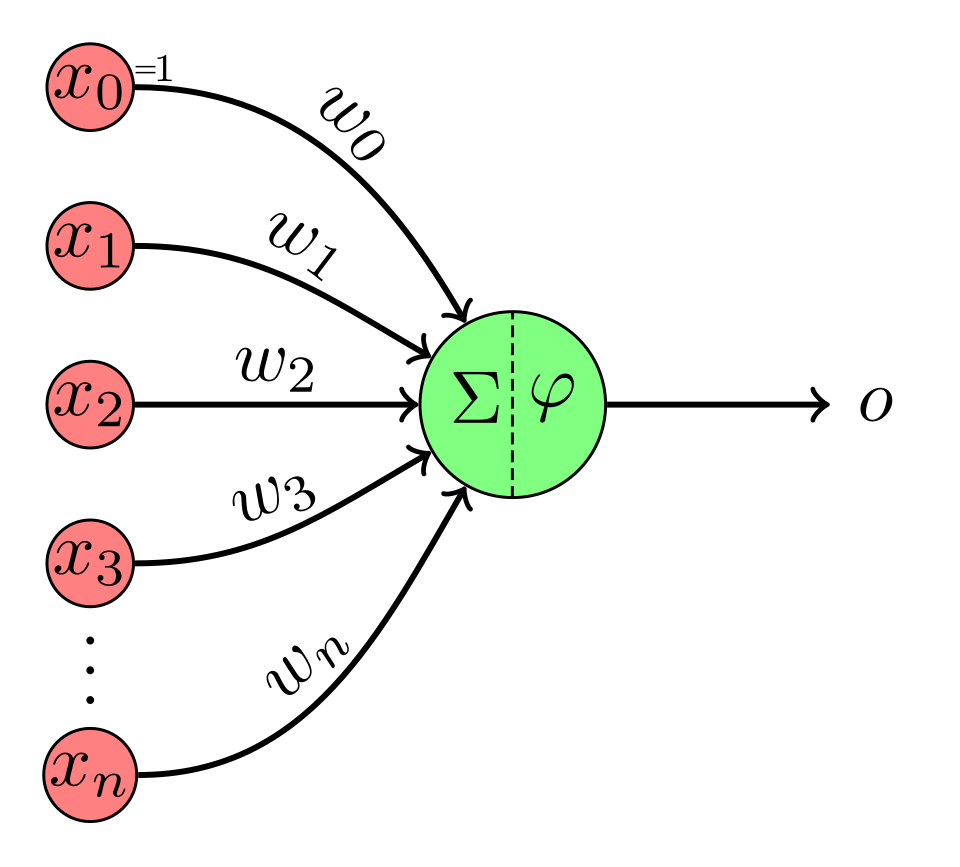
\includegraphics[width=0.68\linewidth]{assets/images/melke-neuronove-site/perceptron-unit.png}
  \caption[Perceptron jako umělý neuron]{Perceptron jako umělý neuron. Popis obrázku: vstupy se násobí
  vahami, sečtou se a výsledná hodnota projde aktivační funkcí. Bias lze chápat jako vstup s konstantní
  hodnotou $1$, který posouvá rozhodovací hranici. Zdroj obrázku: MartinThoma,
  \href{https://commons.wikimedia.org/wiki/File:Perceptron-unit.svg}{Wikimedia Commons}, licence CC0 1.0.}
  \label{fig:perceptron-unit}
\end{figure}

\subsection*{Perceptron pro binární klasifikaci}

U jednoduchého perceptronu se často používá skoková aktivační funkce:
\[
\phi(z)
=
\begin{cases}
1, & z\geq 0,\\
0, & z<0.
\end{cases}
\]

Predikce:
\[
\hat{y}
=
\phi(w^\top x+b).
\]

Perceptron vytváří lineární rozhodovací hranici:
\[
w^\top x+b=0.
\]

To znamená, že jednoduchý perceptron řeší pouze lineárně separovatelné úlohy.

\subsection*{Architektura mělké neuronové sítě}

Mělká dopředná síť s jednou skrytou vrstvou:

\[
x
\rightarrow
h
\rightarrow
\hat{y}.
\]

Pro $H$ neuronů ve skryté vrstvě:

\[
z_j^{(1)}
=
\sum_{\ell=1}^p
w_{j\ell}^{(1)}x_\ell
+
b_j^{(1)},
\qquad
j=1,\ldots,H.
\]

Aktivace skrytých neuronů:
\[
h_j
=
\phi(z_j^{(1)}).
\]

Výstupní vrstva:
\[
z^{(2)}
=
\sum_{j=1}^H
w_j^{(2)}h_j
+
b^{(2)}.
\]

Výstup:
\[
\hat{y}
=
g(z^{(2)}),
\]
kde $g$ závisí na typu úlohy.

Pokud je každá jednotka jedné vrstvy propojena se všemi jednotkami další vrstvy, mluví se o plně propojené
vrstvě. U tabulkových dat je to běžný výchozí model: vstupní proměnné nejprve vytvoří skryté reprezentace a
výstupní vrstva je převede na číselnou predikci nebo pravděpodobnosti tříd.

\begin{figure}[htbp]
  \centering
  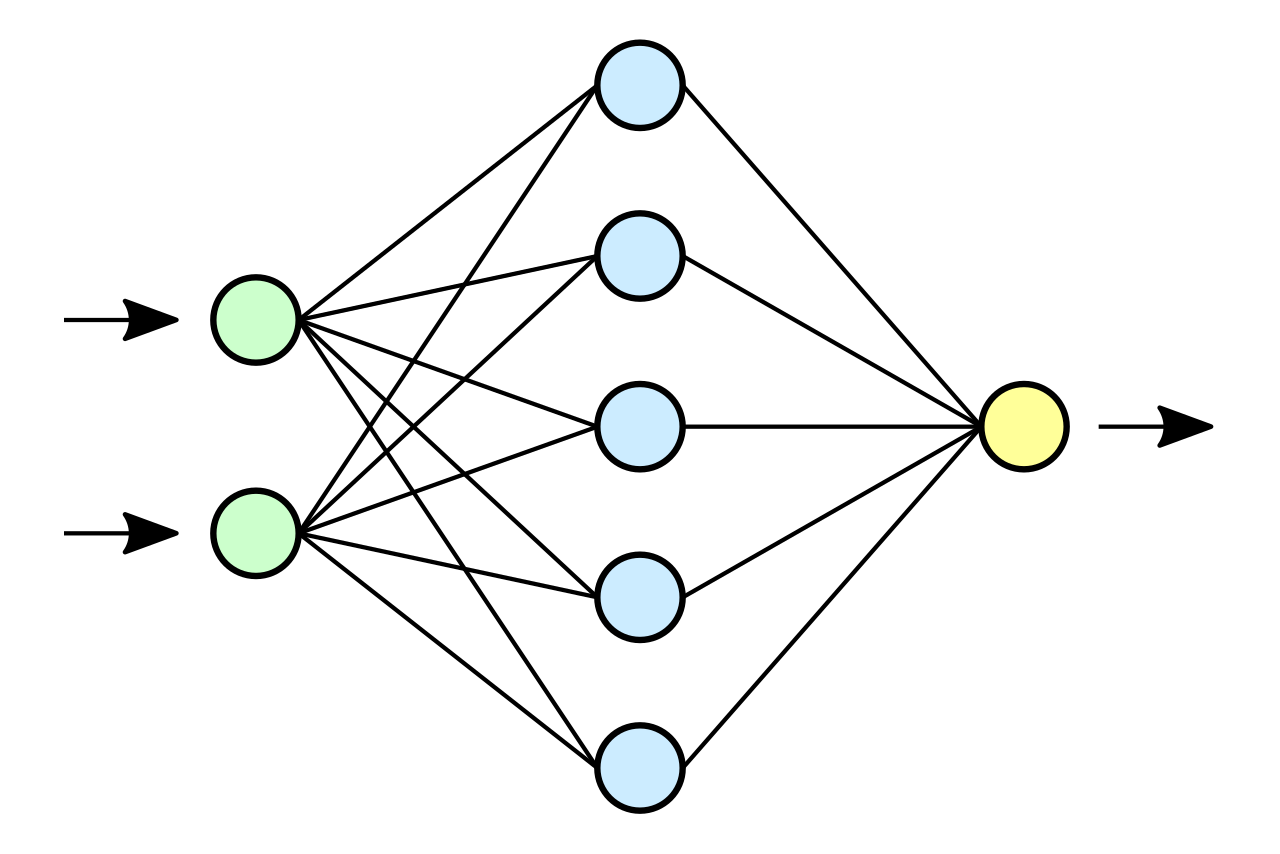
\includegraphics[width=0.74\linewidth]{assets/images/melke-neuronove-site/shallow-neural-network.png}
  \caption[Mělká dopředná neuronová síť]{Zjednodušené schéma dopředné neuronové sítě. Popis obrázku:
  signál teče zleva doprava ze vstupních proměnných přes skrytou vrstvu do výstupu. U mělké sítě je klíčová
  právě jedna skrytá vrstva; přidáním dalších skrytých vrstev vzniká hlubší architektura. Zdroj obrázku:
  Dake a Mysid, \href{https://commons.wikimedia.org/wiki/File:Neural\_network.svg}{Wikimedia Commons},
  licence CC BY 1.0.}
  \label{fig:shallow-neural-network}
\end{figure}

\subsection*{Maticový zápis}

Pro jednu skrytou vrstvu:

\[
h
=
\phi(W^{(1)}x+b^{(1)}),
\]

\[
\hat{y}
=
g(W^{(2)}h+b^{(2)}).
\]

Kde:
\begin{itemize}
    \item $W^{(1)}$ jsou váhy mezi vstupem a skrytou vrstvou,
    \item $b^{(1)}$ jsou biasy skryté vrstvy,
    \item $W^{(2)}$ jsou váhy mezi skrytou a výstupní vrstvou,
    \item $b^{(2)}$ je bias výstupní vrstvy.
\end{itemize}

\subsection*{Aktivační funkce}

Aktivační funkce zavádí nelinearitu. Bez nelineární aktivace by vícevrstvá neuronová síť byla jen lineární
model.

Dobrá aktivační funkce má být nelineární, numericky stabilní a ideálně má poskytovat použitelné gradienty
pro učení. V hidden vrstvách se dnes často používá ReLU nebo její varianty, zatímco sigmoid a softmax se
typicky objevují ve výstupní vrstvě klasifikačních modelů.

\begin{figure}[htbp]
  \centering
  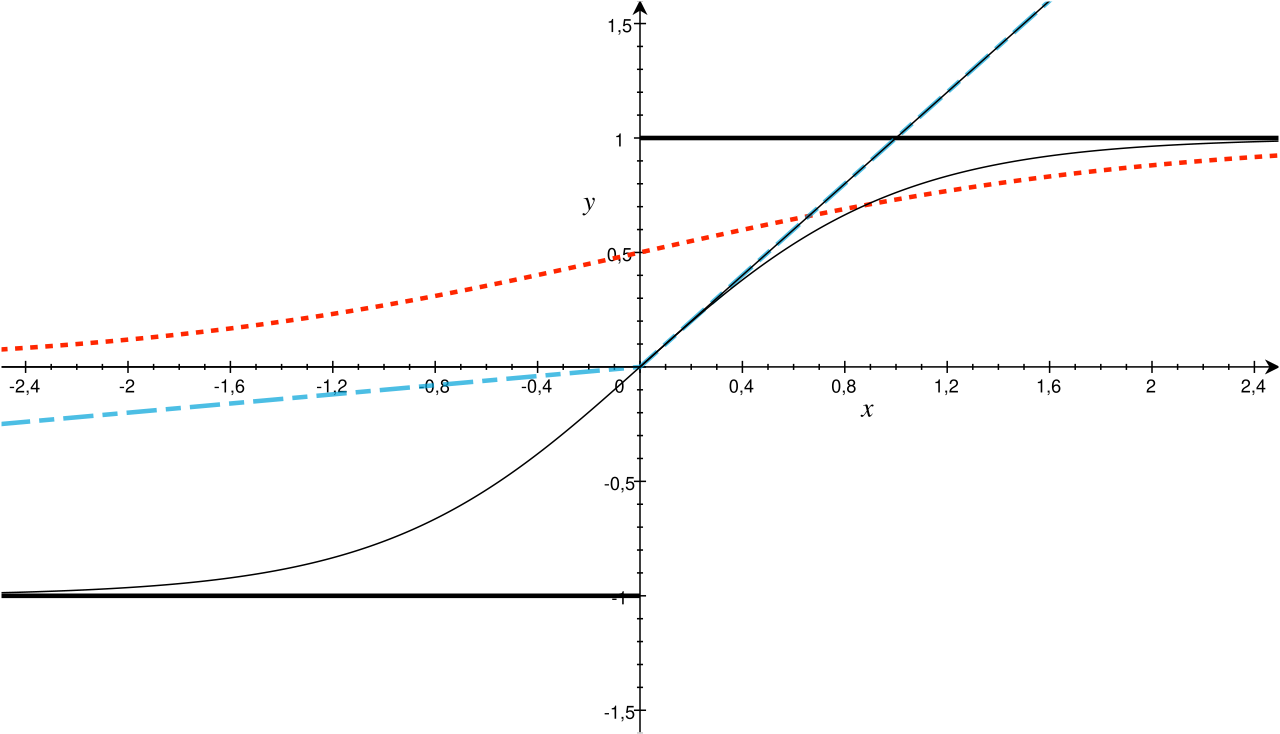
\includegraphics[width=0.86\linewidth]{assets/images/melke-neuronove-site/activation-functions.png}
  \caption[Aktivační funkce]{Příklady aktivačních funkcí. Popis obrázku: sigmoid převádí hodnoty do intervalu
  $(0,1)$, hyperbolický tangens do intervalu $(-1,1)$, ReLU propouští kladné hodnoty a záporné nastavuje na
  nulu. Volba aktivace ovlivňuje nelinearitu modelu i chování gradientů při trénování. Zdroj obrázku:
  Andreas Maier, Christopher Syben, Tobias Lasser a Christian Riess,
  \href{https://commons.wikimedia.org/wiki/File:ActivationFunctions.svg}{Wikimedia Commons}, licence CC BY 4.0.}
  \label{fig:activation-functions}
\end{figure}

\subsubsection*{Sigmoid}

\[
\sigma(z)=
\frac{1}{1+e^{-z}}.
\]

Vlastnosti:
\begin{itemize}
    \item výstup je v intervalu $(0,1)$,
    \item vhodná pro binární výstup,
    \item může trpět vanishing gradient problémem.
\end{itemize}

Derivace:
\[
\sigma'(z)
=
\sigma(z)(1-\sigma(z)).
\]

\subsubsection*{Tanh}

\[
\tanh(z)=
\frac{e^z-e^{-z}}{e^z+e^{-z}}.
\]

Výstup je v intervalu:
\[
(-1,1).
\]

\subsubsection*{ReLU}

\[
ReLU(z)=
\max(0,z).
\]

Výhody:
\begin{itemize}
    \item jednoduchá,
    \item rychlá,
    \item často dobře funguje,
    \item omezuje problém mizejících gradientů oproti sigmoidu.
\end{itemize}

Nevýhoda:
\begin{itemize}
    \item pro záporné hodnoty má nulový gradient, neuron může přestat učit.
\end{itemize}

\subsubsection*{Softmax}

Softmax se používá pro vícetřídní klasifikaci:
\[
\hat{p}_k
=
\frac{e^{z_k}}
{\sum_{\ell=1}^K e^{z_\ell}}.
\]

Platí:
\[
0\leq \hat{p}_k\leq 1,
\qquad
\sum_{k=1}^K \hat{p}_k=1.
\]

\subsection*{Volba výstupní vrstvy podle typu úlohy}

\begin{itemize}
    \item \textbf{Regrese:}
    lineární výstup
    \[
    \hat{y}=z.
    \]
    
    \item \textbf{Binární klasifikace:}
    sigmoid
    \[
    \hat{p}=P(y=1|x)=\sigma(z).
    \]
    
    \item \textbf{Vícetřídní klasifikace:}
    softmax
    \[
    \hat{p}_k=P(y=k|x).
    \]
\end{itemize}

\subsection*{Ztrátové funkce}

Neuronová síť se trénuje minimalizací ztrátové funkce:
\[
L(y,\hat{y}).
\]

Celková empirická ztráta:
\[
J(\theta)
=
\frac{1}{n}
\sum_{i=1}^n
L(y_i,\hat{y}_i),
\]
kde $\theta$ označuje všechny váhy a biasy v síti.

\subsubsection*{MSE pro regresi}

\[
L(y,\hat{y})
=
(y-\hat{y})^2.
\]

Celkově:
\[
MSE
=
\frac{1}{n}
\sum_{i=1}^n
(y_i-\hat{y}_i)^2.
\]

\subsubsection*{Binární cross-entropy}

Pro binární klasifikaci:
\[
L(y,\hat{p})
=
-
\left[
y\log(\hat{p})
+
(1-y)\log(1-\hat{p})
\right].
\]

\subsubsection*{Categorical cross-entropy}

Pro vícetřídní klasifikaci:
\[
L(y,\hat{p})
=
-
\sum_{k=1}^K
y_k\log(\hat{p}_k).
\]

\subsection*{Forward propagation}

Forward propagation znamená výpočet predikce od vstupu k výstupu.

Pro jedno pozorování:
\[
z^{(1)}=W^{(1)}x+b^{(1)},
\]
\[
h=\phi(z^{(1)}),
\]
\[
z^{(2)}=W^{(2)}h+b^{(2)},
\]
\[
\hat{y}=g(z^{(2)}).
\]

Potom spočítáme ztrátu:
\[
L(y,\hat{y}).
\]

\subsection*{Backpropagation}

Backpropagation je algoritmus pro efektivní výpočet gradientů ztrátové funkce podle všech vah a biasů.

Cílem je získat:
\[
\frac{\partial J}{\partial w}
\]
pro každou váhu $w$ v síti.

Používá se řetězové pravidlo:
\[
\frac{\partial L}{\partial w}
=
\frac{\partial L}{\partial \hat{y}}
\cdot
\frac{\partial \hat{y}}{\partial z}
\cdot
\frac{\partial z}{\partial w}.
\]

\paragraph{Intuice.}
Nejprve síť udělá predikci. Spočítáme chybu. Potom chybu propagujeme zpět sítí a zjišťujeme, které váhy
k chybě přispěly a jak je upravit.

Pro síť s jednou skrytou vrstvou lze zpětný průchod zapsat kompaktně. Označme chybu ve výstupní vrstvě:
\[
\delta^{(2)}
=
\frac{\partial L}{\partial z^{(2)}}.
\]
Gradienty pro výstupní vrstvu jsou:
\[
\frac{\partial L}{\partial W^{(2)}}=\delta^{(2)}h^\top,
\qquad
\frac{\partial L}{\partial b^{(2)}}=\delta^{(2)}.
\]
Chyba se do skryté vrstvy přenese přes váhy výstupní vrstvy:
\[
\delta^{(1)}
=
\left(W^{(2)\top}\delta^{(2)}\right)
\odot
\phi'(z^{(1)}),
\]
kde $\odot$ značí násobení po složkách. Gradienty pro první vrstvu jsou:
\[
\frac{\partial L}{\partial W^{(1)}}=\delta^{(1)}x^\top,
\qquad
\frac{\partial L}{\partial b^{(1)}}=\delta^{(1)}.
\]

U kombinace softmaxu a cross-entropy se výstupní chyba zjednoduší na tvar
\[
\delta^{(2)}=\hat{p}-y,
\]
což je jeden z důvodů, proč se tato dvojice v klasifikaci používá tak často.

\subsection*{Gradient descent}

Trénování znamená hledání vah, které minimalizují ztrátovou funkci:
\[
\min_{\theta} J(\theta).
\]

Gradient descent aktualizuje parametry proti směru gradientu:
\[
\theta^{(t+1)}
=
\theta^{(t)}
-
\eta
\nabla J(\theta^{(t)}).
\]

Kde:
\begin{itemize}
    \item $\eta$ je learning rate,
    \item $\nabla J(\theta)$ je gradient ztrátové funkce.
\end{itemize}

Pro jednu váhu:
\[
w^{(t+1)}
=
w^{(t)}
-
\eta
\frac{\partial J}{\partial w}.
\]

\paragraph{Intuice.}
Gradient ukazuje směr nejrychlejšího růstu ztráty. Proto se při minimalizaci pohybujeme opačným směrem.

Optimalizace neuronové sítě je zpravidla nekonvexní. Algoritmus proto nemusí najít globální minimum; v praxi
se hledá dostatečně dobré řešení, které dobře generalizuje na nová data. Důležité je sledovat nejen trénovací
ztrátu, ale i validační ztrátu.

\begin{figure}[htbp]
  \centering
  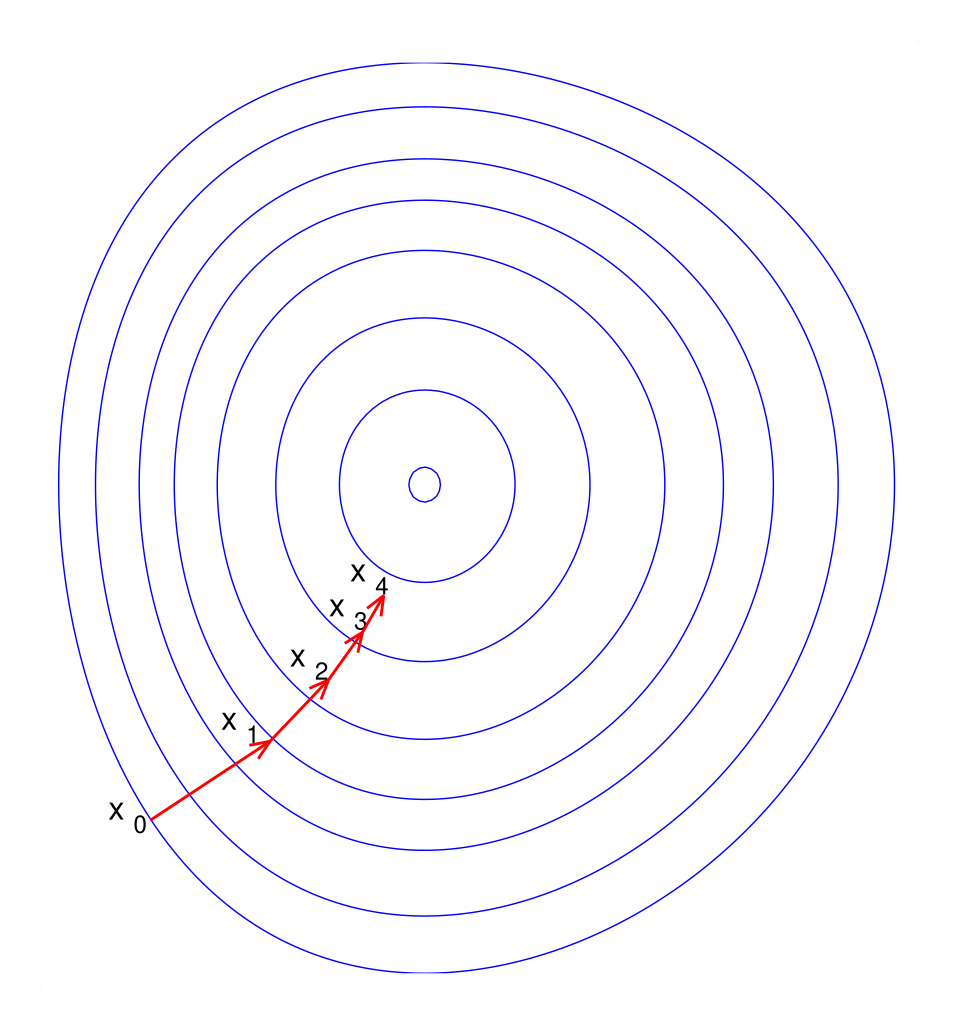
\includegraphics[width=0.58\linewidth]{assets/images/melke-neuronove-site/gradient-descent.png}
  \caption[Gradientní sestup]{Ilustrace gradientního sestupu. Popis obrázku: algoritmus postupně mění
  parametry ve směru, který snižuje hodnotu optimalizované funkce. U neuronových sítí se stejný princip
  používá pro aktualizaci vah podle gradientu ztrátové funkce. Zdroj obrázku: Zerodamage,
  \href{https://commons.wikimedia.org/wiki/File:Gradient\_descent.svg}{Wikimedia Commons}, public domain.}
  \label{fig:gradient-descent}
\end{figure}

\subsection*{Learning rate}

Learning rate $\eta$ určuje velikost kroku.

Pokud je $\eta$ příliš malé:
\begin{itemize}
    \item učení je velmi pomalé,
    \item model může potřebovat mnoho iterací.
\end{itemize}

Pokud je $\eta$ příliš velké:
\begin{itemize}
    \item optimalizace může oscilovat,
    \item ztráta nemusí klesat,
    \item algoritmus může divergovat.
\end{itemize}

\subsection*{Epochy, batch a mini-batch}

\begin{itemize}
    \item \textbf{Epoch:}
    jeden průchod celým trénovacím datasetem.
    
    \item \textbf{Batch:}
    část dat použitá pro jeden update vah.
    
    \item \textbf{Batch size:}
    počet pozorování v jedné dávce.
\end{itemize}

\subsection*{Varianty gradientního sestupu}

\subsubsection*{Batch gradient descent}

Používá celý dataset pro jeden update:
\[
\nabla J(\theta)
=
\frac{1}{n}
\sum_{i=1}^n
\nabla L_i(\theta).
\]

Výhody:
\begin{itemize}
    \item stabilní směr gradientu,
    \item hladší konvergence.
\end{itemize}

Nevýhody:
\begin{itemize}
    \item pomalé pro velká data,
    \item vysoká paměťová náročnost.
\end{itemize}

\subsubsection*{Stochastic gradient descent}

Používá jedno pozorování:
\[
\theta
\leftarrow
\theta
-
\eta
\nabla L_i(\theta).
\]

Výhody:
\begin{itemize}
    \item rychlé aktualizace,
    \item může pomoci uniknout z lokálních minim.
\end{itemize}

Nevýhody:
\begin{itemize}
    \item kolísavá konvergence,
    \item citlivost na learning rate.
\end{itemize}

\subsubsection*{Mini-batch gradient descent}

Používá malou dávku dat:
\[
B\subset \{1,\ldots,n\}.
\]

\[
\theta
\leftarrow
\theta
-
\eta
\frac{1}{|B|}
\sum_{i\in B}
\nabla L_i(\theta).
\]

Je to nejběžnější varianta v praxi.

\subsection*{Momentum}

Momentum vyhlazuje aktualizace a zrychluje pohyb ve stabilním směru.

\[
v_t
=
\gamma v_{t-1}
+
\eta \nabla J(\theta_t),
\]
\[
\theta_{t+1}
=
\theta_t-v_t.
\]

Momentum pomáhá omezit oscilace a zrychlit konvergenci.

\subsection*{Adaptivní optimalizátory}

\subsubsection*{AdaGrad}

AdaGrad upravuje learning rate pro každý parametr podle historie gradientů. Parametry s velkými gradienty
dostávají menší kroky.

\subsubsection*{RMSprop}

RMSprop používá exponenciálně vážený průměr čtverců gradientů, čímž řeší příliš rychlé snižování learning
rate u AdaGrad.

\subsubsection*{Adam}

Adam kombinuje momentum a adaptivní learning rate. Udržuje:
\begin{itemize}
    \item odhad prvního momentu gradientu,
    \item odhad druhého momentu gradientu.
\end{itemize}

Pro gradient $g_t=\nabla J(\theta_t)$ platí zjednodušeně:
\[
m_t=\beta_1m_{t-1}+(1-\beta_1)g_t,
\]
\[
v_t=\beta_2v_{t-1}+(1-\beta_2)g_t^2.
\]
Po korekci počátečního vychýlení se parametry aktualizují přibližně jako
\[
\theta_{t+1}
=
\theta_t
-
\eta
\frac{\hat{m}_t}{\sqrt{\hat{v}_t}+\varepsilon}.
\]

V praxi je Adam velmi často používaný optimalizátor.

\subsection*{Newtonova metoda a vztah k optimalizaci}

Newtonova metoda využívá nejen gradient, ale i druhou derivaci, tedy křivost funkce.

Pro jednu proměnnou:
\[
x_{t+1}
=
x_t
-
\frac{f'(x_t)}{f''(x_t)}.
\]

U více proměnných:
\[
\theta_{t+1}
=
\theta_t
-
H^{-1}
\nabla J(\theta_t),
\]
kde $H$ je Hessian.

Výhoda:
\begin{itemize}
    \item může konvergovat rychleji.
\end{itemize}

Nevýhody:
\begin{itemize}
    \item výpočet Hessianu je drahý,
    \item metoda je citlivá na počáteční hodnoty,
    \item u velkých neuronových sítí je často nepraktická.
\end{itemize}

Proto se v neuronových sítích používají hlavně gradientní metody, mini-batch trénování a optimalizátory jako
Adam.

\subsection*{Počet neuronů ve skryté vrstvě}

Počet neuronů je důležitý hyperparametr.

Příliš málo neuronů:
\[
\Rightarrow
\text{underfitting}.
\]

Příliš mnoho neuronů:
\[
\Rightarrow
\text{overfitting}.
\]

Praktický postup:
\begin{itemize}
    \item začít jednodušším modelem,
    \item postupně přidávat neurony,
    \item sledovat validační chybu,
    \item použít cross-validation nebo validační množinu.
\end{itemize}

\subsection*{Inicializace vah}

Váhy se typicky inicializují náhodně, ale ne příliš velké ani všechny stejné.

Pokud by všechny váhy byly stejné, neurony ve stejné vrstvě by se učily totéž. Náhodná inicializace rozbíjí
symetrii.

\subsection*{Regularizace a prevence přeučení}

Neuronové sítě se mohou snadno přeučit.

Možnosti prevence:
\begin{itemize}
    \item menší počet neuronů,
    \item regularizace vah,
    \item early stopping,
    \item dropout,
    \item více trénovacích dat,
    \item augmentace dat,
    \item validace na oddělených datech.
\end{itemize}

Dropout při trénování náhodně vypíná část neuronů, takže se síť nemůže příliš spoléhat na konkrétní jednotky.
Při predikci se používá celá síť se správným škálováním aktivací. U mělkých sítí se dropout používá méně
často než u hlubokých modelů, ale princip je důležitý: snižuje závislost modelu na jednotlivých vahách.

L2 regularizace:
\[
J_{\lambda}(\theta)
=
J(\theta)
+
\lambda
\sum_j w_j^2.
\]

L1 regularizace:
\[
J_{\lambda}(\theta)
=
J(\theta)
+
\lambda
\sum_j |w_j|.
\]

\subsection*{Early stopping}

Sledujeme chybu na validační množině:
\[
Err_{\text{val}}.
\]

Pokud trénovací chyba dál klesá, ale validační chyba začne růst, model se přeučuje.

\[
Err_{\text{train}}\downarrow
\quad
\text{a}
\quad
Err_{\text{val}}\uparrow
\quad
\Rightarrow
\quad
\text{zastavit trénování}.
\]

V praxi se nastavuje také \term{patience}, tedy kolik epoch bez zlepšení validační chyby ještě tolerujeme.
Early stopping je jednoduchá, ale silná regularizační technika, protože vybere model před začátkem výrazného
přeučení.

\subsection*{Vanishing a exploding gradient}

Vanishing gradient znamená, že gradienty při zpětné propagaci postupně mizí:
\[
\left|
\frac{\partial L}{\partial w}
\right|
\approx 0.
\]

Potom se váhy v dřívějších vrstvách učí velmi pomalu nebo vůbec. Problém je častější u hlubokých sítí a
aktivačních funkcí jako sigmoid nebo tanh.

Řešení:
\begin{itemize}
    \item ReLU a její varianty,
    \item vhodná inicializace vah,
    \item normalizace,
    \item reziduální architektury u hlubokých sítí.
\end{itemize}

U mělkých sítí je problém menší, ale princip je důležitý pro pochopení trénování.

Opačným problémem je \term{exploding gradient}, kdy jsou gradienty příliš velké a aktualizace vah začnou
divergovat. Pomáhá menší learning rate, vhodná inicializace, normalizace a u některých modelů také
\term{gradient clipping}, tedy omezení maximální velikosti gradientu.

\subsection*{Praktický workflow trénování}

\begin{enumerate}
    \item připravit data a odstranit/řešit missing values,
    \item zakódovat kategoriální proměnné,
    \item standardizovat numerické proměnné,
    \item rozdělit data na train/validation/test,
    \item zvolit architekturu sítě,
    \item zvolit aktivační funkce,
    \item zvolit loss function,
    \item zvolit optimalizátor a learning rate,
    \item trénovat model,
    \item sledovat train a validation chybu,
    \item ladit hyperparametry,
    \item finálně vyhodnotit na testovacích datech.
\end{enumerate}

U neuronových sítí je zvlášť důležité škálování vstupů. Standardizaci nebo normalizaci je potřeba naučit jen
na trénovacích datech a stejnou transformaci použít na validační a testovací data. Pokud by se scaler fitoval
i na testovací množině, šlo by o únik informace z testu do trénování.

\paragraph{Typické hyperparametry.}
\begin{itemize}
    \item počet neuronů ve skryté vrstvě,
    \item aktivační funkce,
    \item learning rate,
    \item batch size,
    \item počet epoch nebo early stopping,
    \item regularizační parametr,
    \item volba optimalizátoru.
\end{itemize}

\subsection*{Výhody a nevýhody mělkých neuronových sítí}

Výhody:
\begin{itemize}
    \item umí zachytit nelineární vztahy,
    \item použitelné pro regresi i klasifikaci,
    \item flexibilní architektura,
    \item základ pro pochopení hlubokého učení.
\end{itemize}

Nevýhody:
\begin{itemize}
    \item horší interpretovatelnost než regrese nebo stromy,
    \item nutnost ladit mnoho hyperparametrů,
    \item citlivost na škálování dat,
    \item riziko přeučení,
    \item optimalizace může skončit v horším lokálním řešení.
\end{itemize}

\subsection*{Co si pamatovat u zkoušky}

\begin{itemize}
    \item Perceptron je lineární kombinace vstupů, bias a aktivační funkce.
    \item Bez nelineární aktivace by síť byla jen lineární model.
    \item Mělká síť má jednu skrytou vrstvu; hluboká síť má více skrytých vrstev.
    \item Forward propagation počítá predikci, backpropagation počítá gradienty.
    \item Gradient descent a jeho varianty upravují váhy proti směru gradientu.
    \item Klasifikace obvykle používá cross-entropy, regrese MSE.
    \item Model je citlivý na škálování vstupů, learning rate a regularizaci.
\end{itemize}

\subsection*{Shrnutí ke zkoušce}

Mělká neuronová síť má vstupní vrstvu, jednu skrytou vrstvu a výstupní vrstvu. Každý neuron počítá lineární
kombinaci vstupů a aplikuje aktivační funkci:
\[
a=\phi(w^\top x+b).
\]

Díky aktivačním funkcím je síť schopna modelovat nelineární vztahy. Predikce se počítá dopředným průchodem
a chyba se minimalizuje pomocí ztrátové funkce. Backpropagation efektivně vypočítá gradienty a optimalizátor
upravuje váhy:
\[
w^{(t+1)}
=
w^{(t)}
-
\eta
\frac{\partial J}{\partial w}.
\]

Důležité jsou volba architektury, aktivačních funkcí, loss function, learning rate, optimalizátoru a prevence
přeučení. Mělké sítě jsou flexibilní, ale méně interpretovatelné a citlivé na správné nastavení.

\subsection*{Zdroje}

\begin{itemize}
    \item scikit-learn User Guide:
    \href{https://scikit-learn.org/stable/modules/neural\_networks\_supervised.html}{Neural network models
    (supervised)}.
    \item scikit-learn API Reference:
    \href{https://scikit-learn.org/stable/modules/generated/sklearn.neural\_network.MLPClassifier.html}{MLPClassifier}.
    \item Goodfellow, Bengio, Courville:
    \href{https://www.deeplearningbook.org/}{Deep Learning}.
    \item Wikimedia Commons:
    \href{https://commons.wikimedia.org/wiki/File:Perceptron-unit.svg}{Perceptron-unit}.
    \item Wikimedia Commons:
    \href{https://commons.wikimedia.org/wiki/File:Neural\_network.svg}{Neural network}.
    \item Wikimedia Commons:
    \href{https://commons.wikimedia.org/wiki/File:ActivationFunctions.svg}{ActivationFunctions}.
    \item Wikimedia Commons:
    \href{https://commons.wikimedia.org/wiki/File:Gradient\_descent.svg}{Gradient descent}.
\end{itemize}

\newpage

\section{Vícevrstvé neuronové sítě a hluboké učení. Koncepce, aplikace, technologie}

\subsection*{Základní vymezení}

\textbf{Neuronová síť} je model složený z propojených výpočetních jednotek -- neuronů. Každý neuron počítá
vážený součet vstupů, přičte bias a použije aktivační funkci:
\[
z = w^\top x + b,
\qquad
a = \phi(z).
\]

Vícevrstvá neuronová síť skládá takových transformací více za sebou:
\[
x
\rightarrow
h^{(1)}
\rightarrow
h^{(2)}
\rightarrow
\cdots
\rightarrow
\hat y.
\]

\textbf{Hluboké učení} je část strojového učení založená na neuronových sítích s více skrytými vrstvami.
Hluboké sítě se neučí jen přímý vztah mezi vstupem a výstupem, ale postupně se učí reprezentace dat.
Nižší vrstvy zachycují jednoduché rysy, vyšší vrstvy složitější struktury.

\paragraph{Intuice.}
U obrázku mohou první vrstvy detekovat hrany a jednoduché tvary, další vrstvy části objektů a poslední vrstvy
celé objekty. U textu mohou první vrstvy zachycovat tokeny/slova, další vrstvy syntaktické a významové vztahy.

\subsection*{Mělká vs. hluboká síť}

\begin{itemize}
    \item \textbf{Mělká síť} má typicky jednu skrytou vrstvu.
    \item \textbf{Hluboká síť} má více skrytých vrstev.
    \item Více vrstev umožňuje skládat jednoduché nelineární transformace do složitějších funkcí.
    \item Hluboké sítě jsou výkonné hlavně pro nestrukturovaná data: obraz, text, zvuk, video.
\end{itemize}

Obecný tvar dopředné hluboké sítě:
\[
h^{(0)} = x,
\]
\[
z^{(\ell)} = W^{(\ell)}h^{(\ell-1)} + b^{(\ell)},
\qquad
h^{(\ell)} = \phi^{(\ell)}(z^{(\ell)}),
\qquad
\ell=1,\ldots,L.
\]

Výstup:
\[
\hat y = g(z^{(L)}),
\]
kde $g$ závisí na úloze:
\begin{itemize}
    \item regrese: lineární výstup,
    \item binární klasifikace: sigmoid,
    \item vícetřídní klasifikace: softmax.
\end{itemize}

\subsection*{Proč hluboké učení funguje}

Hluboké sítě jsou úspěšné hlavně díky kombinaci několika faktorů:
\begin{itemize}
    \item dostupnost velkých datasetů,
    \item vyšší výpočetní výkon, hlavně GPU/TPU,
    \item lepší optimalizační algoritmy,
    \item lepší inicializace vah,
    \item regularizace a normalizace,
    \item specializované architektury jako CNN, RNN a transformery,
    \item transfer learning a předtrénované modely.
\end{itemize}

\paragraph{Důležité.}
Hluboké učení není vhodné vždy. U malých tabulkových datasetů mohou být lepší jednodušší modely, například
logistická regrese, rozhodovací strom, random forest nebo gradient boosting. Hluboké sítě se vyplatí hlavně
tam, kde je hodně dat a složitá struktura vstupu.

\subsection*{Vícevrstvý perceptron}

Vícevrstvý perceptron, MLP, je základní dopředná neuronová síť. Každý neuron jedné vrstvy je typicky spojen
se všemi neurony následující vrstvy. Takovým vrstvám se říká plně propojené vrstvy:
\[
\text{Dense layer}.
\]

Pro jednu skrytou vrstvu:
\[
h = \phi(W^{(1)}x+b^{(1)}),
\]
\[
\hat y = g(W^{(2)}h+b^{(2)}).
\]

Pro více skrytých vrstev:
\[
h^{(1)} = \phi(W^{(1)}x+b^{(1)}),
\]
\[
h^{(2)} = \phi(W^{(2)}h^{(1)}+b^{(2)}),
\]
\[
\hat y = g(W^{(3)}h^{(2)}+b^{(3)}).
\]

\subsection*{Počet parametrů v hustých vrstvách}

Počet parametrů mezi dvěma plně propojenými vrstvami:
\[
(n_{\text{in}}+1)n_{\text{out}},
\]
kde $+1$ odpovídá biasu.

\paragraph{Příklad MNIST.}
Obrázek má velikost:
\[
28 \times 28 = 784
\]
vstupních hodnot. Pokud má síť jednu skrytou vrstvu s 256 neurony a výstupní vrstvu s 10 neurony, počet
parametrů je:
\[
784\cdot 256 + 256 + 256\cdot 10 + 10 = 203530.
\]

To ukazuje, že počet parametrů rychle roste. Proto se u obrázků nepoužívají pouze husté vrstvy, ale hlavně
konvoluční sítě.

\subsection*{Aktivační funkce}

Aktivační funkce zavádějí nelinearitu. Bez nich by složení více vrstev bylo opět jen lineární transformací.

\subsubsection*{Sigmoid}

\[
\sigma(z)=\frac{1}{1+e^{-z}}.
\]

Použití:
\begin{itemize}
    \item binární klasifikace,
    \item výstup jako pravděpodobnost.
\end{itemize}

Nevýhoda:
\begin{itemize}
    \item pro velká kladná/záporná $z$ má velmi malý gradient, což může vést k problému mizejícího gradientu.
\end{itemize}

\subsubsection*{Tanh}

\[
\tanh(z)=\frac{e^z-e^{-z}}{e^z+e^{-z}}.
\]

Výstup je v intervalu:
\[
(-1,1).
\]

\subsubsection*{ReLU}

\[
\operatorname{ReLU}(z)=\max(0,z).
\]

Výhody:
\begin{itemize}
    \item jednoduchá,
    \item výpočetně rychlá,
    \item často funguje lépe ve skrytých vrstvách než sigmoid/tanh,
    \item zmírňuje problém mizejícího gradientu.
\end{itemize}

Nevýhoda:
\begin{itemize}
    \item pro záporné vstupy má nulový gradient; neuron může přestat učit.
\end{itemize}

\subsubsection*{Softmax}

Softmax se používá pro vícetřídní klasifikaci:
\[
\hat p_k =
\frac{e^{z_k}}
{\sum_{j=1}^{K} e^{z_j}}.
\]

Platí:
\[
0 \leq \hat p_k \leq 1,
\qquad
\sum_{k=1}^{K}\hat p_k=1.
\]

\subsection*{Ztrátové funkce}

Neuronová síť se učí minimalizací ztrátové funkce:
\[
J(\theta)
=
\frac{1}{n}
\sum_{i=1}^n
L(y_i,\hat y_i),
\]
kde $\theta$ označuje všechny váhy a biasy.

\subsubsection*{Regrese}

Pro regresi se často používá MSE:
\[
L(y,\hat y)=(y-\hat y)^2.
\]

Celkově:
\[
MSE=
\frac{1}{n}
\sum_{i=1}^{n}
(y_i-\hat y_i)^2.
\]

\subsubsection*{Binární klasifikace}

Binary cross-entropy:
\[
L(y,\hat p)
=
-\left[
y\log(\hat p)
+
(1-y)\log(1-\hat p)
\right].
\]

\subsubsection*{Vícetřídní klasifikace}

Categorical cross-entropy:
\[
L(y,\hat p)
=
-\sum_{k=1}^{K} y_k\log(\hat p_k),
\]
kde $y_k$ je one-hot reprezentace skutečné třídy.

\subsection*{Trénování hlubokých sítí}

Trénování znamená hledání parametrů, které minimalizují ztrátovou funkci:
\[
\min_{\theta} J(\theta).
\]

Nejčastěji se používají gradientní metody:
\[
\theta^{(t+1)}
=
\theta^{(t)}
-
\eta \nabla J(\theta^{(t)}),
\]
kde $\eta$ je learning rate.

\subsubsection*{Forward propagation}

Dopředný průchod spočítá predikci:
\[
x \rightarrow \hat y.
\]

Například:
\[
z^{(1)}=W^{(1)}x+b^{(1)},
\]
\[
h^{(1)}=\phi(z^{(1)}),
\]
\[
z^{(2)}=W^{(2)}h^{(1)}+b^{(2)},
\]
\[
\hat y=g(z^{(2)}).
\]

\subsubsection*{Backpropagation}

Backpropagation efektivně počítá derivace ztráty podle všech vah pomocí řetězového pravidla:
\[
\frac{\partial L}{\partial w}
=
\frac{\partial L}{\partial \hat y}
\cdot
\frac{\partial \hat y}{\partial z}
\cdot
\frac{\partial z}{\partial w}.
\]

\paragraph{Intuice.}
Síť nejprve udělá predikci, poté spočítá chybu a následně šíří informaci o chybě zpět přes jednotlivé vrstvy.
Každá váha se upraví podle toho, jak přispěla k chybě.

\subsection*{Gradientní optimalizátory}

\subsubsection*{Batch gradient descent}

Používá celý trénovací dataset pro jeden update:
\[
\nabla J(\theta)
=
\frac{1}{n}
\sum_{i=1}^{n}
\nabla L_i(\theta).
\]

Výhoda:
\begin{itemize}
    \item stabilní gradient.
\end{itemize}

Nevýhoda:
\begin{itemize}
    \item pomalé u velkých datasetů.
\end{itemize}

\subsubsection*{Stochastic gradient descent}

Aktualizuje parametry po jednom pozorování:
\[
\theta
\leftarrow
\theta
-
\eta \nabla L_i(\theta).
\]

Výhody:
\begin{itemize}
    \item rychlé aktualizace,
    \item šum v gradientu může pomoci uniknout z horších lokálních minim.
\end{itemize}

Nevýhody:
\begin{itemize}
    \item nestabilnější konvergence,
    \item citlivost na learning rate.
\end{itemize}

\subsubsection*{Mini-batch gradient descent}

Používá malou dávku pozorování:
\[
B\subset \{1,\ldots,n\}.
\]

Aktualizace:
\[
\theta
\leftarrow
\theta
-
\eta
\frac{1}{|B|}
\sum_{i\in B}
\nabla L_i(\theta).
\]

Toto je nejběžnější varianta pro hluboké učení.

\subsubsection*{Momentum}

Momentum používá informaci o předchozích gradientech:
\[
v_t = \gamma v_{t-1} + \eta \nabla J(\theta_t),
\]
\[
\theta_{t+1} = \theta_t - v_t.
\]

Pomáhá zrychlit učení ve stabilním směru a tlumit oscilace.

\subsubsection*{Adam}

Adam kombinuje momentum a adaptivní learning rate. Udržuje odhad prvního a druhého momentu gradientů.
V praxi je jedním z nejpoužívanějších optimalizátorů pro neuronové sítě.

\subsection*{Problémy při trénování}

\subsubsection*{Mizející gradient}

Mizející gradient znamená:
\[
\left|
\frac{\partial L}{\partial w}
\right|
\approx 0.
\]

Potom se váhy v nižších vrstvách téměř neučí. Problém je častý u hlubokých sítí a aktivačních funkcí
sigmoid/tanh.

Řešení:
\begin{itemize}
    \item ReLU a její varianty,
    \item vhodná inicializace vah,
    \item batch normalization,
    \item reziduální spojení,
    \item LSTM/GRU u sekvenčních dat.
\end{itemize}

\subsubsection*{Explodující gradient}

Explodující gradient znamená, že gradienty jsou příliš velké:
\[
\left|
\frac{\partial L}{\partial w}
\right|
\gg 1.
\]

Řešení:
\begin{itemize}
    \item gradient clipping,
    \item menší learning rate,
    \item lepší inicializace,
    \item normalizace.
\end{itemize}

\subsubsection*{Overfitting}

Hluboké sítě mají mnoho parametrů, a proto se mohou přeučit:
\[
Err_{\text{train}} \ll Err_{\text{test}}.
\]

Řešení:
\begin{itemize}
    \item větší dataset,
    \item regularizace,
    \item dropout,
    \item early stopping,
    \item data augmentation,
    \item jednodušší architektura,
    \item transfer learning.
\end{itemize}

\subsection*{Regularizace}

\subsubsection*{L2 regularizace}

\[
J_{\lambda}(\theta)
=
J(\theta)
+
\lambda
\sum_j w_j^2.
\]

L2 penalizuje velké váhy a tím omezuje složitost modelu.

\subsubsection*{L1 regularizace}

\[
J_{\lambda}(\theta)
=
J(\theta)
+
\lambda
\sum_j |w_j|.
\]

L1 může vést k řídkým modelům, protože některé váhy tlačí k nule.

\subsubsection*{Dropout}

Dropout náhodně vypíná část neuronů během trénování:
\[
\tilde h = m \odot h,
\qquad
m_j \sim \operatorname{Bernoulli}(q).
\]

Model se tím učí nebýt příliš závislý na konkrétních neuronech.

\subsubsection*{Batch normalization}

Batch normalization normalizuje aktivace v dávce:
\[
\hat x =
\frac{x-\mu_B}
{\sqrt{\sigma_B^2+\varepsilon}},
\]
\[
y=\gamma \hat x+\beta.
\]

Pomáhá stabilizovat a zrychlit trénování.

\subsubsection*{Early stopping}

Sledujeme validační chybu:
\[
Err_{\text{val}}.
\]

Pokud trénovací chyba klesá, ale validační chyba začne růst, model se začíná přeučovat:
\[
Err_{\text{train}}\downarrow
\quad
\text{a}
\quad
Err_{\text{val}}\uparrow.
\]

Trénování zastavíme v bodě s nejlepší validační chybou.

\subsection*{Konvoluční neuronové sítě}

Konvoluční neuronové sítě, CNN, jsou specializované hlavně na obrazová data. Obrázek lze chápat jako tensor:
\begin{itemize}
    \item černobílý obrázek: výška $\times$ šířka,
    \item barevný RGB obrázek: výška $\times$ šířka $\times$ 3,
    \item dávka obrázků: počet obrázků $\times$ výška $\times$ šířka $\times$ počet kanálů.
\end{itemize}

Například RGB batch:
\[
(256,128,128,3).
\]

\subsection*{Proč nestačí plně propojené vrstvy pro obrázky}

U obrázku $32\times 32\times 3$ máme:
\[
32\cdot 32\cdot 3=3072
\]
vstupů. Pokud by byl každý neuron ve skryté vrstvě propojen se všemi pixely, počet parametrů by rychle
rostl. Navíc by síť nevyužívala prostorovou strukturu obrázku.

CNN používají:
\begin{itemize}
    \item lokální propojení,
    \item sdílení parametrů,
    \item konvoluční filtry,
    \item pooling,
    \item hierarchickou extrakci příznaků.
\end{itemize}

\subsection*{Konvoluce}

Konvoluce aplikuje filtr, také kernel, na vstupní obrázek a vytváří feature mapu:
\[
S(i,j)=(I*K)(i,j).
\]

Pro více kanálů a více filtrů:
\[
S_{i,j,k}
=
\phi
\left(
b_k+
\sum_{u=1}^{F_h}
\sum_{v=1}^{F_w}
\sum_{c=1}^{C_{\text{in}}}
K_{u,v,c,k}X_{i+u,j+v,c}
\right).
\]

Kde:
\begin{itemize}
    \item $X$ je vstupní obrázek nebo aktivace předchozí vrstvy,
    \item $K$ je konvoluční filtr,
    \item $S$ je výstupní feature mapa,
    \item $C_{\text{in}}$ je počet vstupních kanálů,
    \item $C_{\text{out}}$ je počet filtrů, tedy počet výstupních kanálů.
\end{itemize}

\subsection*{Velikost výstupu konvoluce}

Pro výšku:
\[
H_{\text{out}}
=
\left\lfloor
\frac{H+2P-F_h}{s_h}
\right\rfloor
+1.
\]

Pro šířku:
\[
W_{\text{out}}
=
\left\lfloor
\frac{W+2P-F_w}{s_w}
\right\rfloor
+1.
\]

Kde:
\begin{itemize}
    \item $H,W$ jsou rozměry vstupu,
    \item $F_h,F_w$ rozměry filtru,
    \item $P$ padding,
    \item $s_h,s_w$ stride.
\end{itemize}

\subsection*{Počet parametrů v konvoluční vrstvě}

Počet trénovatelných parametrů:
\[
F_hF_wC_{\text{in}}C_{\text{out}}+C_{\text{out}}.
\]

První část jsou váhy filtrů, druhá část biasy.

\paragraph{Příklad.}
Konvoluce s filtrem $3\times 3$, jedním vstupním kanálem a 32 filtry má:
\[
3\cdot 3\cdot 1\cdot 32 + 32 = 320
\]
parametrů.

\subsection*{Pooling}

Pooling zmenšuje prostorové rozměry:
\[
H\times W \rightarrow H'\times W'.
\]

Nejčastější je max pooling, například filtr $2\times 2$ se stride 2:
\[
\max
\begin{pmatrix}
x_{11} & x_{12}\\
x_{21} & x_{22}
\end{pmatrix}.
\]

Pooling:
\begin{itemize}
    \item snižuje počet hodnot,
    \item zmenšuje výpočetní náročnost,
    \item zvyšuje určitou robustnost vůči malým posunům,
    \item obvykle nemá trénovatelné parametry.
\end{itemize}

\subsection*{Typická CNN architektura}

Základní konvoluční síť:
\[
\text{Input}
\rightarrow
\text{Convolution}
\rightarrow
\text{ReLU}
\rightarrow
\text{Pooling}
\rightarrow
\text{Convolution}
\rightarrow
\text{ReLU}
\rightarrow
\text{Pooling}
\rightarrow
\text{Flatten}
\rightarrow
\text{Dense}
\rightarrow
\text{Softmax}.
\]

\paragraph{Příklad MNIST CNN.}
\[
(28,28,1)
\rightarrow
(26,26,32)
\rightarrow
(13,13,32)
\rightarrow
(11,11,64)
\rightarrow
(5,5,64)
\rightarrow
(3,3,128)
\rightarrow
(1152,)
\rightarrow
(10,).
\]

Počet parametrů:
\[
3\cdot3\cdot1\cdot32+32
+
3\cdot3\cdot32\cdot64+64
+
3\cdot3\cdot64\cdot128+128
+
3\cdot3\cdot128\cdot10+10
=
104202.
\]

\subsection*{Data augmentation}

Data augmentation uměle rozšiřuje trénovací data transformacemi, které nemění třídu objektu.

U obrázků:
\begin{itemize}
    \item otočení,
    \item posun,
    \item změna měřítka,
    \item ořez,
    \item horizontální překlopení,
    \item šum,
    \item změna jasu nebo kontrastu.
\end{itemize}

\paragraph{Intuice.}
Pes zůstává psem i po mírném otočení nebo ořezu obrázku. Model se tím učí robustnější reprezentace.

Existují dva přístupy:
\begin{itemize}
    \item \textbf{offline augmentation} -- nové obrázky se předem uloží na disk,
    \item \textbf{on-the-fly augmentation} -- transformace se generují během trénování.
\end{itemize}

\subsection*{Moderní CNN architektury}

\begin{itemize}
    \item \textbf{LeNet} -- raná CNN pro rozpoznávání číslic.
    \item \textbf{AlexNet} -- významný úspěch v počítačovém vidění, využití hlubší sítě a GPU.
    \item \textbf{VGG} -- jednoduchá architektura s mnoha $3\times 3$ konvolucemi.
    \item \textbf{Inception / GoogLeNet} -- paralelní konvoluce různých velikostí, efektivní využití parametrů.
    \item \textbf{ResNet} -- reziduální spojení, umožňuje trénovat velmi hluboké sítě.
\end{itemize}

Reziduální blok:
\[
h^{(\ell+1)}
=
F(h^{(\ell)}) + h^{(\ell)}.
\]

Reziduální spojení pomáhá toku gradientu a řeší problém, že velmi hluboké sítě se jinak obtížně trénují.

\subsection*{Rekurentní neuronové sítě}

Rekurentní neuronové sítě, RNN, jsou určeny pro sekvenční data:
\[
x_1,x_2,\ldots,x_T.
\]

Příklady:
\begin{itemize}
    \item text,
    \item řeč,
    \item časové řady,
    \item DNA sekvence,
    \item video.
\end{itemize}

U sekvenčních dat záleží na pořadí. RNN umožňuje, aby zpracování aktuálního prvku záviselo na předchozí
historii.

\subsection*{Vstupní tensor u RNN}

Pro jednu sekvenci:
\[
(x_1,\ldots,x_T),
\]
kde $x_t$ je vektor příznaků v čase $t$.

Pro mini-batch:
\[
(\text{batch size},\text{time steps},\text{features}).
\]

\subsection*{Jednoduchá RNN}

Skrytý stav:
\[
h_t = f_h(W_hh_{t-1}+W_xx_t+b).
\]

Výstup:
\[
y_t = f_o(W_oh_t+c).
\]

Kde:
\begin{itemize}
    \item $h_t$ shrnuje dosavadní historii,
    \item $x_t$ je aktuální vstup,
    \item stejné váhy se používají ve všech časových krocích.
\end{itemize}

\paragraph{Sdílení parametrů.}
RNN používá stejné matice $W_h,W_x,W_o$ pro každý časový krok. Díky tomu může zpracovávat sekvence různé délky.

\subsection*{Typy RNN úloh}

\begin{itemize}
    \item \textbf{One-to-one:}
    jeden vstup a jeden výstup, běžná dopředná síť.
    
    \item \textbf{Many-to-one:}
    sekvence na jeden výstup, například sentiment věty.
    
    \item \textbf{One-to-many:}
    jeden vstup na sekvenci výstupů, například generování popisu obrázku.
    
    \item \textbf{Many-to-many:}
    sekvence na sekvenci, například strojový překlad nebo značkování slov ve větě.
\end{itemize}

\subsection*{Problémy jednoduchých RNN}

Jednoduché RNN mají problém s dlouhodobými závislostmi.

\begin{itemize}
    \item \textbf{Vanishing gradient:}
    informace z dávné minulosti se při zpětném šíření ztrácí.
    
    \item \textbf{Exploding gradient:}
    gradienty mohou prudce růst.
    
    \item \textbf{Sekvenční výpočet:}
    časové kroky se zpracovávají postupně, což omezuje paralelizaci.
\end{itemize}

Řešení:
\begin{itemize}
    \item LSTM,
    \item GRU,
    \item bidirectional RNN,
    \item attention mechanismus,
    \item transformery.
\end{itemize}

\subsection*{LSTM}

LSTM, Long Short-Term Memory, používá paměťovou buňku a brány, které řídí tok informací.

Forget gate:
\[
f_t = \sigma(W_f[h_{t-1},x_t]+b_f).
\]

Input gate:
\[
i_t = \sigma(W_i[h_{t-1},x_t]+b_i).
\]

Kandidátní paměť:
\[
\tilde c_t = \tanh(W_c[h_{t-1},x_t]+b_c).
\]

Aktualizace paměti:
\[
c_t = f_t\odot c_{t-1}+i_t\odot \tilde c_t.
\]

Output gate:
\[
o_t = \sigma(W_o[h_{t-1},x_t]+b_o).
\]

Nový skrytý stav:
\[
h_t = o_t\odot \tanh(c_t).
\]

\paragraph{Intuice.}
LSTM se učí, co zapomenout, co přidat do paměti a co poslat dál jako výstup. Díky tomu lépe zachycuje
dlouhodobé závislosti než jednoduchá RNN.

\subsection*{GRU}

GRU, Gated Recurrent Unit, je jednodušší varianta bránové RNN.

Update gate:
\[
z_t = \sigma(W_z[h_{t-1},x_t]+b_z).
\]

Reset gate:
\[
r_t = \sigma(W_r[h_{t-1},x_t]+b_r).
\]

Kandidátní stav:
\[
\tilde h_t =
\tanh(W_h[r_t\odot h_{t-1},x_t]+b_h).
\]

Nový stav:
\[
h_t =
(1-z_t)\odot h_{t-1}
+
z_t\odot \tilde h_t.
\]

GRU má méně parametrů než LSTM, a proto může být rychlejší.

\subsection*{Bidirectional RNN}

Bidirectional RNN zpracovává sekvenci oběma směry:
\[
\overrightarrow{h_t}
\quad \text{z minulosti do budoucnosti},
\]
\[
\overleftarrow{h_t}
\quad \text{z budoucnosti do minulosti}.
\]

Výstup může používat:
\[
h_t =
[\overrightarrow{h_t},\overleftarrow{h_t}].
\]

Použití:
\begin{itemize}
    \item rozpoznávání řeči,
    \item rozpoznávání rukopisu,
    \item bioinformatika,
    \item zpracování textu, kde známe celou větu.
\end{itemize}

\subsection*{Word embeddings}

Text nelze přímo vložit do neuronové sítě jako slova. Je potřeba převod slov na vektory.

\subsubsection*{One-hot encoding}

Každé slovo je reprezentováno dlouhým řídkým vektorem:
\[
\text{pes} = (0,0,1,0,\ldots,0).
\]

Nevýhody:
\begin{itemize}
    \item vysoká dimenze,
    \item řídkost,
    \item žádná informace o významové podobnosti slov.
\end{itemize}

\subsubsection*{Embedding}

Embedding je hustý nízkorozměrný vektor:
\[
\text{pes} \mapsto e_{\text{pes}}\in \mathbb{R}^d.
\]

Podobná slova by měla mít podobné vektory. Podobnost lze měřit například kosinovou podobností:
\[
\cos(e_i,e_j)=
\frac{e_i^\top e_j}
{\|e_i\|\|e_j\|}.
\]

\subsubsection*{Word2Vec}

Word2Vec se učí reprezentace slov z kontextu.

\begin{itemize}
    \item \textbf{CBOW:}
    z okolních slov predikuje prostřední slovo.
    
    \item \textbf{Skip-gram:}
    z daného slova predikuje okolní slova.
\end{itemize}

Skip-gram bývá vhodnější pro méně častá slova a menší trénovací data. CBOW se obvykle trénuje rychleji.

\subsection*{Transformery}

Transformery jsou architektury založené na mechanismu attention. Vznikly jako řešení omezení RNN:
\begin{itemize}
    \item RNN zpracovávají sekvenci postupně,
    \item obtížně zachycují dlouhé závislosti,
    \item trpí mizejícím gradientem,
    \item hůře se paralelizují.
\end{itemize}

Transformer reprezentuje prvky sekvence podle jejich vzájemné relevance.

\subsection*{Self-attention}

Máme sekvenci reprezentovanou maticí:
\[
X\in \mathbb{R}^{n\times d}.
\]

Z ní se vytvoří:
\[
Q=XW_Q,
\qquad
K=XW_K,
\qquad
V=XW_V.
\]

Kde:
\begin{itemize}
    \item $Q$ jsou queries,
    \item $K$ jsou keys,
    \item $V$ jsou values.
\end{itemize}

Scaled dot-product attention:
\[
\operatorname{Attention}(Q,K,V)
=
\operatorname{softmax}
\left(
\frac{QK^\top}{\sqrt{d_k}}
\right)
V.
\]

\paragraph{Intuice.}
Každý token se ptá, na které ostatní tokeny se má dívat. Podobnost query a key určuje váhu. Výsledkem je
vážený součet value vektorů.

\subsection*{Multi-head attention}

Místo jedné attention se použije více hlav:
\[
\operatorname{head}_i
=
\operatorname{Attention}
(QW_i^Q,KW_i^K,VW_i^V).
\]

Výstup:
\[
\operatorname{MultiHead}(Q,K,V)
=
\operatorname{Concat}(\operatorname{head}_1,\ldots,\operatorname{head}_h)W^O.
\]

Každá hlava se může naučit jiný typ vztahu v sekvenci.

\subsection*{Pozicové kódování}

Self-attention sama o sobě nezná pořadí tokenů. Proto se přidává pozicové kódování:
\[
X_{\text{input}} = X_{\text{embedding}} + X_{\text{position}}.
\]

Bez pozicového kódování by transformer nerozlišil, zda slovo stojí na začátku nebo na konci věty.

\subsection*{Encoder-decoder transformer}

Původní transformer pro strojový překlad má dvě části:

\begin{itemize}
    \item \textbf{Encoder:}
    převádí vstupní sekvenci na kontextové reprezentace.
    
    \item \textbf{Decoder:}
    generuje výstupní sekvenci autoregresivně, tedy postupně token po tokenu.
\end{itemize}

V encoderu se používá self-attention nad vstupem. V decoderu se používá:
\begin{itemize}
    \item masked self-attention, aby model neviděl budoucí tokeny,
    \item attention nad výstupem encoderu,
    \item feed-forward vrstvy.
\end{itemize}

\subsection*{Typy transformerových modelů}

\begin{itemize}
    \item \textbf{Encoder-only:}
    vhodné pro porozumění textu, klasifikaci, extrakci informací.
    Příklad: BERT.
    
    \item \textbf{Decoder-only:}
    vhodné pro generování textu.
    Příklad: GPT modely.
    
    \item \textbf{Encoder-decoder:}
    vhodné pro překlad, sumarizaci a transformaci jedné sekvence na druhou.
    Příklad: T5.
\end{itemize}

\subsection*{Předtrénování a transfer learning}

Hluboké modely často netrénujeme od nuly. Používáme předtrénované modely:
\[
\theta_{\text{pretrained}}.
\]

Poté je upravíme pro konkrétní úlohu:
\[
\theta_{\text{fine-tuned}}.
\]

\subsubsection*{Transfer learning u CNN}

U obrázků se často použije předtrénovaná CNN jako extraktor příznaků:
\[
x \rightarrow \text{CNN backbone} \rightarrow z.
\]

Potom přidáme novou klasifikační hlavu:
\[
z \rightarrow \text{Dense} \rightarrow \hat y.
\]

Možnosti:
\begin{itemize}
    \item zmrazit původní vrstvy a trénovat jen novou hlavu,
    \item částečně odemrazit vyšší vrstvy,
    \item fine-tunovat celý model s malým learning rate.
\end{itemize}

\subsubsection*{Self-supervised learning}

U velkých jazykových modelů se často využívá self-supervised učení. Model si vytváří cílovou proměnnou z
dat samotných.

Příklady:
\begin{itemize}
    \item predikce dalšího tokenu,
    \item predikce maskovaného tokenu,
    \item kontrastivní učení reprezentací.
\end{itemize}

\subsection*{Autoencodery}

Autoencoder je neuronová síť, která se učí rekonstruovat vlastní vstup:
\[
x \rightarrow z \rightarrow \hat x.
\]

Encoder:
\[
z=f_{\theta}(x).
\]

Decoder:
\[
\hat x=g_{\phi}(z).
\]

Ztráta:
\[
L(x,\hat x)=\|x-\hat x\|^2.
\]

\paragraph{Bottleneck.}
Nejužší skrytá vrstva se nazývá code nebo bottleneck. Pokud má malou dimenzi, autoencoder se musí naučit
kompaktní reprezentaci dat.

Použití:
\begin{itemize}
    \item redukce dimenze,
    \item vizualizace dat,
    \item denoising,
    \item detekce anomálií,
    \item inicializace reprezentací.
\end{itemize}

\subsection*{Denoising autoencoder}

Denoising autoencoder dostane zašuměný vstup:
\[
\tilde x = x + \varepsilon,
\]
ale učí se rekonstruovat původní vstup:
\[
\hat x \approx x.
\]

Tím se učí robustnější reprezentace.

\subsection*{Aplikace hlubokého učení}

\subsubsection*{Obrazová data}

\begin{itemize}
    \item klasifikace obrázků,
    \item detekce objektů,
    \item segmentace obrazu,
    \item OCR,
    \item medicínské snímky,
    \item detekce porušování lidských práv z obrazových dat,
    \item kontrola kvality ve výrobě,
    \item autonomní řízení.
\end{itemize}

\subsubsection*{Text a jazyk}

\begin{itemize}
    \item sentiment analysis,
    \item strojový překlad,
    \item sumarizace,
    \item vyhledávání informací,
    \item otázky a odpovědi,
    \item klasifikace dokumentů,
    \item extrakce entit,
    \item generování textu.
\end{itemize}

\subsubsection*{Zvuk a řeč}

\begin{itemize}
    \item rozpoznávání řeči,
    \item převod textu na řeč,
    \item detekce řečníka,
    \item klasifikace zvuků,
    \item zpracování hudby.
\end{itemize}

\subsubsection*{Časové řady}

\begin{itemize}
    \item predikce poptávky,
    \item predikce spotřeby energie,
    \item detekce anomálií,
    \item prediktivní údržba,
    \item finanční časové řady,
    \item senzory a IoT.
\end{itemize}

\subsubsection*{Business aplikace}

\begin{itemize}
    \item detekce fraudu,
    \item scoring zákazníků,
    \item churn prediction,
    \item doporučovací systémy,
    \item automatizace zákaznické podpory,
    \item personalizovaný marketing,
    \item analýza clickstreamů.
\end{itemize}

\subsection*{Technologie pro hluboké učení}

\subsubsection*{Programovací jazyky a knihovny}

Nejčastější technologie:
\begin{itemize}
    \item \textbf{Python} -- hlavní jazyk pro deep learning,
    \item \textbf{NumPy, pandas} -- práce s daty,
    \item \textbf{scikit-learn} -- klasické ML a preprocessing,
    \item \textbf{TensorFlow / Keras} -- tvorba a trénování neuronových sítí,
    \item \textbf{PyTorch} -- flexibilní framework, často používaný ve výzkumu i produkci,
    \item \textbf{Hugging Face Transformers} -- předtrénované NLP a transformerové modely,
    \item \textbf{OpenCV} -- počítačové vidění.
\end{itemize}

\subsubsection*{Hardware}

Hluboké sítě jsou výpočetně náročné. Používají se:
\begin{itemize}
    \item CPU pro menší úlohy,
    \item GPU pro paralelní výpočty matic a tensorů,
    \item TPU pro specializované trénování neuronových sítí,
    \item distribuované clustery pro velké modely.
\end{itemize}

GPU zrychluje zejména operace:
\[
XW,
\qquad
\text{konvoluce},
\qquad
\text{backpropagation}.
\]

\subsubsection*{Datové pipeline}

Pro úspěšné hluboké učení nestačí jen model. Je potřeba i spolehlivá datová pipeline:
\begin{itemize}
    \item načítání dat,
    \item čištění dat,
    \item transformace,
    \item augmentace,
    \item batching,
    \item caching,
    \item monitoring kvality dat.
\end{itemize}

\subsubsection*{Nasazení modelu}

Model lze nasadit například jako:
\begin{itemize}
    \item REST API,
    \item batch scoring,
    \item stream processing,
    \item model běžící v mobilní aplikaci,
    \item model v cloudové službě.
\end{itemize}

Produkční řešení typicky vyžaduje:
\begin{itemize}
    \item kontejnerizaci,
    \item modularizaci,
    \item škálování,
    \item správu přístupů a tajemství,
    \item CI/CD,
    \item auditovatelnost,
    \item možnost rollbacku,
    \item monitoring výkonu a driftu.
\end{itemize}

\subsection*{MLOps}

MLOps propojuje vývoj modelu, datové inženýrství a provoz.

Typický proces:
\begin{enumerate}
    \item příprava dat,
    \item trénování modelu,
    \item validace,
    \item registrace modelu,
    \item nasazení,
    \item monitoring,
    \item retrénování,
    \item správa verzí.
\end{enumerate}

\paragraph{Důležité.}
Model v produkci není jednorázový výstup. Časem se mohou měnit data, chování uživatelů i business procesy.
Proto je nutné sledovat:
\begin{itemize}
    \item predikční výkon,
    \item datový drift,
    \item konceptový drift,
    \item latenci,
    \item náklady,
    \item chybovost služby.
\end{itemize}

\subsection*{Evaluace hlubokých modelů}

Model se hodnotí na oddělených datech:
\[
D =
D_{\text{train}}
\cup
D_{\text{validation}}
\cup
D_{\text{test}}.
\]

\begin{itemize}
    \item \textbf{Trénovací data} slouží k učení vah.
    \item \textbf{Validační data} slouží k výběru architektury a hyperparametrů.
    \item \textbf{Testovací data} slouží k finálnímu nezávislému ověření.
\end{itemize}

U klasifikace:
\[
Accuracy,\quad Precision,\quad Recall,\quad F_1,\quad AUC.
\]

U regrese:
\[
MSE,\quad RMSE,\quad MAE.
\]

U generativních modelů je hodnocení obtížnější, protože kromě přesnosti řešíme také kvalitu, užitečnost,
bezpečnost a věcnou správnost výstupu.

\subsection*{Hyperparametry}

Hyperparametry nejsou přímo naučené z dat, ale nastavují se před trénováním.

Typické hyperparametry:
\begin{itemize}
    \item počet vrstev,
    \item počet neuronů,
    \item typ aktivační funkce,
    \item learning rate,
    \item batch size,
    \item počet epoch,
    \item dropout rate,
    \item regularizační koeficient,
    \item typ optimalizátoru,
    \item velikost kernelu u CNN,
    \item počet attention heads u transformeru.
\end{itemize}

Ladění:
\begin{itemize}
    \item grid search,
    \item random search,
    \item Bayesian optimization,
    \item ruční ladění podle learning curves,
    \item early stopping.
\end{itemize}

\subsection*{Interpretovatelnost a vysvětlitelnost}

Neuronové sítě a hluboké modely jsou často \textbf{black-box} modely. Uživatel obvykle nevidí jednoduché
pravidlo, proč model rozhodl právě takto.

Rozlišujeme:
\begin{itemize}
    \item \textbf{globální interpretovatelnost} -- jak model funguje jako celek,
    \item \textbf{lokální interpretovatelnost} -- proč model rozhodl u konkrétního pozorování.
\end{itemize}

Metody vysvětlování:
\begin{itemize}
    \item variable importance,
    \item permutation importance,
    \item partial dependence plots,
    \item ICE plots,
    \item LIME,
    \item SHAP,
    \item surrogate modely,
    \item saliency maps u obrazových modelů,
    \item attention visualization u transformerů.
\end{itemize}

\paragraph{Surrogate model.}
Naučíme jednodušší model, například rozhodovací strom, který aproximuje predikce složitého modelu:
\[
\hat y_{\text{black-box}}
\approx
\hat y_{\text{surrogate}}.
\]

Potom interpretujeme jednodušší model. Je ale nutné kontrolovat fidelitu, tedy jak dobře surrogate skutečně
napodobuje původní model.

\subsection*{Rizika hlubokého učení}

\begin{itemize}
    \item potřeba velkého množství dat,
    \item vysoké výpočetní náklady,
    \item přeučení,
    \item nízká interpretovatelnost,
    \item citlivost na bias v datech,
    \item data leakage,
    \item adversariální příklady,
    \item drift v produkci,
    \item právní a etické požadavky,
    \item riziko nadměrného spoléhání na výstupy AI.
\end{itemize}

U vysoce rizikových aplikací je nutná lidská kontrola, dokumentace, auditovatelnost a možnost zásahu člověka.

\subsection*{Srovnání hlavních architektur}

\begin{itemize}
    \item \textbf{MLP:}
    obecná dopředná síť pro tabulková data a jednoduché úlohy.
    
    \item \textbf{CNN:}
    nejlepší pro obrazová data a úlohy, kde je důležitá lokální struktura.
    
    \item \textbf{RNN/LSTM/GRU:}
    sekvenční modely, vhodné pro text, řeč a časové řady, ale hůře paralelizovatelné.
    
    \item \textbf{Transformer:}
    attention-based architektura, výborná pro jazyk, text, multimodální modely a dlouhé závislosti.
    
    \item \textbf{Autoencoder:}
    model pro učení reprezentací, redukci dimenze, rekonstrukci a detekci anomálií.
\end{itemize}

\subsection*{Co říct u státnic}

Vícevrstvé neuronové sítě skládají více nelineárních transformací za sebou:
\[
h^{(\ell)}
=
\phi(W^{(\ell)}h^{(\ell-1)}+b^{(\ell)}).
\]
Díky tomu se mohou učit složité vztahy a hierarchické reprezentace dat. Hluboké učení je úspěšné hlavně díky
velkým datům, GPU, lepším optimalizačním algoritmům, regularizaci a specializovaným architekturám.

U obrázků se používají CNN, které využívají konvoluce, lokální propojení, sdílení parametrů a pooling.
U sekvenčních dat se používají RNN, LSTM a GRU:
\[
h_t=f_h(W_hh_{t-1}+W_xx_t+b).
\]
Moderní jazykové a generativní modely stojí hlavně na transformerech a self-attention:
\[
\operatorname{Attention}(Q,K,V)
=
\operatorname{softmax}
\left(
\frac{QK^\top}{\sqrt{d_k}}
\right)V.
\]

Hluboké modely se používají pro obraz, text, řeč, časové řady, fraud detection, doporučování nebo automatizaci
business procesů. Prakticky je důležité nejen trénování, ale také příprava dat, validace, MLOps, nasazení,
monitoring, škálování, bezpečnost a interpretovatelnost. Největší slabiny hlubokého učení jsou náročnost na
data a výpočetní výkon, riziko přeučení, black-box povaha a potřeba kontroly biasu, driftu a právních/etických
dopadů.

\newpage
\section{Nestrukturovaná a částečně strukturovaná data. Porovnávání vzorů, indexování a vyhledávání dokumentů, extrakce informací a web scraping}

\subsection*{Základní vymezení}

Data lze podle míry strukturovanosti rozdělit na:
\begin{itemize}
    \item \textbf{strukturovaná data} -- mají pevné schéma, typicky relační tabulky v databázi;
    \item \textbf{semistrukturovaná data} -- mají vnitřní strukturu, ale ta nemusí být pevně tabulková,
    například XML, JSON, HTML nebo logy;
    \item \textbf{nestrukturovaná data} -- nemají pevnou tabulkovou strukturu, například volný text,
    dokumenty, PDF, e-maily, obrázky, audio, video nebo webové stránky.
\end{itemize}

\paragraph{Důležitá poznámka.}
Text se často označuje jako nestrukturovaný, ale není úplně bez struktury. Přirozený jazyk má slova,
věty, gramatiku, syntax, morfologii a významové vztahy. Pro databázový systém ale obvykle nejde o předem
dané řádky a sloupce, a proto se text řadí mezi nestrukturovaná nebo slabě strukturovaná data.

\subsection*{Semistrukturovaná data}

Semistrukturovaná data mají značky, klíče nebo hierarchii, které umožňují obsah strojově zpracovat.
Prakticky je důležité nepřistupovat k nim jako k obyčejnému řetězci, pokud existuje parser pro daný formát:
u XML a HTML je bezpečnější pracovat se stromem dokumentu, u JSONu s objekty a poli.

\subsubsection*{XML}

XML je značkovací jazyk se stromovou strukturou. Data jsou tvořena elementy, atributy a textovým obsahem.

Příklad:
\[
\texttt{<book id="1"><title>Data Mining</title><price>39.90</price></book>}
\]

Vlastnosti XML:
\begin{itemize}
    \item stromová struktura,
    \item značky oddělují jednotlivé části dokumentu,
    \item možnost validace přes DTD nebo XML Schema,
    \item vhodné pro dokumenty, konfigurace a výměnu dat.
\end{itemize}

Pro dotazování nad XML se používají například:
\begin{itemize}
    \item \textbf{XPath} -- výběr uzlů ve stromu,
    \item \textbf{XQuery} -- dotazovací jazyk pro XML dokumenty.
\end{itemize}

\subsubsection*{JSON}

JSON je lehčí formát často používaný ve webových API a dokumentových databázích.

Příklad:
\[
\texttt{\{"id": 1, "title": "Data Mining", "price": 39.90\}}
\]

Vlastnosti JSON:
\begin{itemize}
    \item objekt je množina dvojic klíč--hodnota,
    \item podporuje pole, čísla, řetězce, logické hodnoty a vnořené objekty,
    \item je přirozeně použitelný v JavaScriptu,
    \item používá se v REST API, logování, konfiguracích a NoSQL databázích.
\end{itemize}

Dokumentové databáze, například MongoDB nebo CouchDB, ukládají záznamy právě jako dokumenty podobné JSONu.
Výhodou je flexibilita schématu, nevýhodou slabší kontrola integrity než u dobře navrženého relačního modelu.

\subsubsection*{HTML a DOM}

HTML je značkovací jazyk webových stránek. Pro web scraping je důležitý model DOM:
\[
\text{HTML dokument} \rightarrow \text{DOM strom}.
\]

DOM strom umožňuje vybírat prvky stránky pomocí:
\begin{itemize}
    \item CSS selektorů,
    \item XPath výrazů,
    \item navigace přes rodiče, potomky a sourozence uzlů.
\end{itemize}

Například CSS selektor:
\[
\texttt{div.product span.price}
\]
vybere cenu uvnitř elementu \texttt{span} s třídou \texttt{price}, který je uvnitř produktu.

\begin{figure}[htbp]
  \centering
  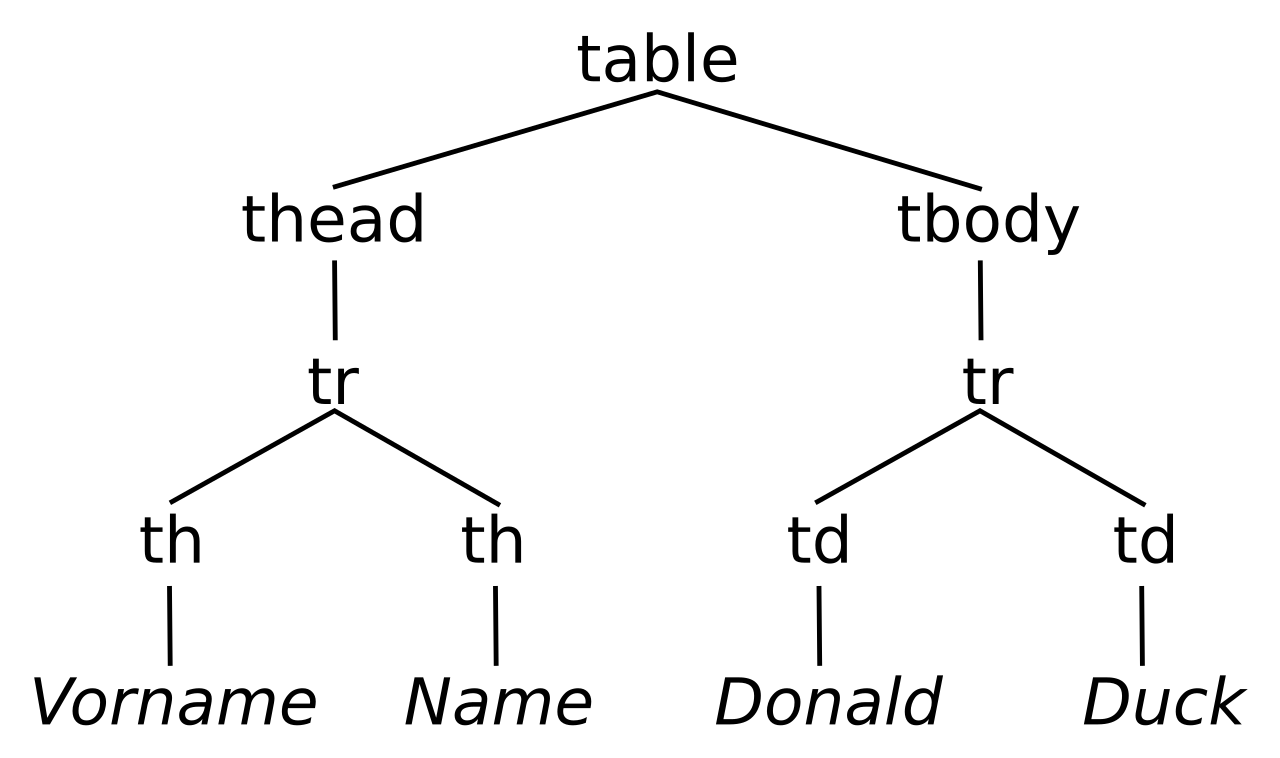
\includegraphics[width=0.70\linewidth]{assets/images/nestrukturovana-data/dom-tree.png}
  \caption[DOM strom HTML dokumentu]{Příklad DOM stromu. Popis obrázku: elementy HTML tabulky tvoří
  hierarchii rodičů a potomků, nad kterou lze vybírat uzly pomocí CSS selektorů, XPath nebo navigace ve
  stromu. Zdroj obrázku: Molily, SVG Marlus Gancher,
  \href{https://commons.wikimedia.org/wiki/File:DOM\_Beispielbaum.svg}{Wikimedia Commons}, public domain.}
  \label{fig:q17-dom-tree}
\end{figure}

\subsection*{Porovnávání vzorů}

Porovnávání vzorů znamená hledání částí dat, které odpovídají určitému předpisu. Může jít o:
\begin{itemize}
    \item přesné porovnání řetězců,
    \item regulární výrazy,
    \item přibližné porovnání řetězců,
    \item podobnost dokumentů nebo embeddingů.
\end{itemize}

\subsection*{Regulární výrazy}

Regulární výraz je formální textový vzor, který umožňuje vyhledávat, validovat, extrahovat nebo nahrazovat
části textu.

Použití:
\begin{itemize}
    \item validace e-mailu, telefonu, PSČ nebo identifikátoru,
    \item extrakce dat, měnových částek, IP adres nebo kódů,
    \item čištění logů,
    \item normalizace textu,
    \item rychlá extrakce jednoduchých entit.
\end{itemize}

\subsubsection*{Základní prvky regulárních výrazů}

\begin{itemize}
    \item \textbf{literál} -- obyčejný znak, například \texttt{a};
    \item \textbf{metaznak} -- znak se speciálním významem;
    \item \textbf{escape} -- zrušení speciálního významu metaznaku;
    \item \textbf{znaková třída} -- množina povolených znaků;
    \item \textbf{kvantifikátor} -- počet opakování;
    \item \textbf{skupina} -- část vzoru uzavřená v závorkách;
    \item \textbf{alternativa} -- výběr jedné z možností.
\end{itemize}

Příklady:
\[
\texttt{\textbackslash d}
\quad
\text{číslice},
\qquad
\texttt{\textbackslash w}
\quad
\text{slovní znak},
\qquad
\texttt{\textbackslash s}
\quad
\text{bílý znak}.
\]

Kvantifikátory:
\[
\texttt{*}
\quad
\text{0 nebo více výskytů},
\qquad
\texttt{+}
\quad
\text{1 nebo více výskytů},
\qquad
\texttt{?}
\quad
\text{0 nebo 1 výskyt}.
\]

Začátek a konec řetězce:
\[
\texttt{\string^}
\quad
\text{začátek},
\qquad
\texttt{\$}
\quad
\text{konec}.
\]

\subsubsection*{Příklad extrakce částky}

Chceme najít částky typu:
\[
\texttt{23 MEUR},\quad \texttt{500 EUR},\quad \texttt{17 KEUR}.
\]

Regex:
\[
\texttt{(\textbackslash d+)\textbackslash s*(MEUR|KEUR|EUR)}
\]

Význam:
\begin{itemize}
    \item \texttt{(\textbackslash d+)} -- jedna nebo více číslic, první zachycená skupina;
    \item \texttt{\textbackslash s*} -- libovolný počet mezer;
    \item \texttt{(MEUR|KEUR|EUR)} -- jedna z měnových jednotek.
\end{itemize}

\subsubsection*{Lookaround}

Lookaround umožňuje kontrolovat okolí nalezeného výrazu, aniž by se toto okolí stalo součástí výsledku.

\begin{itemize}
    \item \textbf{positive lookahead}: výraz musí následovat;
    \item \textbf{negative lookahead}: výraz nesmí následovat;
    \item \textbf{positive lookbehind}: výraz musí předcházet;
    \item \textbf{negative lookbehind}: výraz nesmí předcházet.
\end{itemize}

Například chceme najít číslo jen tehdy, pokud za ním následuje \texttt{EUR}:
\[
\texttt{\textbackslash d+(?=\textbackslash s*EUR)}
\]

\subsubsection*{Silné a slabé stránky regexů}

Výhody:
\begin{itemize}
    \item rychlé a přesné pro formální vzory,
    \item dobré pro kódy, data, měny, ID, e-maily, logy,
    \item jednoduché nasazení bez trénovacích dat.
\end{itemize}

Nevýhody:
\begin{itemize}
    \item špatně zachycují význam a kontext,
    \item pro přirozený jazyk bývají křehké,
    \item složité regexy jsou málo čitelné,
    \item při změně formátu dat se snadno rozbijí.
\end{itemize}

\paragraph{Typická chyba.}
Regex je vhodný pro jednoduchý textový vzor, ale není dobrý obecný parser HTML nebo XML. U webových stránek je
spolehlivější nejprve vytvořit DOM strom a až potom vybírat konkrétní elementy.

\subsection*{Přibližné porovnávání řetězců}

Přibližné porovnávání řetězců řeší situace, kdy texty nejsou totožné, ale jsou podobné:
\[
\texttt{international}
\quad
\text{vs.}
\quad
\texttt{internationalization}.
\]

Typické míry:
\begin{itemize}
    \item \textbf{Hammingova vzdálenost} -- počet rozdílných znaků na stejných pozicích;
    \item \textbf{Levenshteinova vzdálenost} -- minimální počet vložení, smazání a nahrazení;
    \item \textbf{Jaro-Winkler} -- vhodné pro jména a krátké řetězce;
    \item \textbf{nejdelší společná podposloupnost} -- délka nejdelší posloupnosti zachované v obou textech.
\end{itemize}

Levenshteinova vzdálenost:
\[
d(i,j)=
\min
\begin{cases}
d(i-1,j)+1,\\
d(i,j-1)+1,\\
d(i-1,j-1)+I(x_i\neq y_j).
\end{cases}
\]

Použití:
\begin{itemize}
    \item deduplikace záznamů,
    \item fuzzy matching jmen,
    \item opravy překlepů,
    \item propojení dat z různých zdrojů.
\end{itemize}

\subsection*{Information Retrieval}

Information Retrieval, zkráceně IR, je oblast zabývající se vyhledáváním relevantních dokumentů v kolekci
textů. Uživatel formuluje informační potřebu jako dotaz a systém vrací dokumenty nebo pasáže, které dotazu
odpovídají.

\paragraph{Základní architektura IR systému.}
\[
\begin{aligned}
\text{kolekce dokumentů}
&\rightarrow
\text{indexer}
\rightarrow
\text{index},\\
\text{uživatelský dotaz}
&\rightarrow
\text{query operations}
\rightarrow
\text{spustitelný dotaz},\\
\text{index + dotaz}
&\rightarrow
\text{retrieval system}
\rightarrow
\text{seřazené dokumenty}.
\end{aligned}
\]

\begin{figure}[htbp]
  \centering
  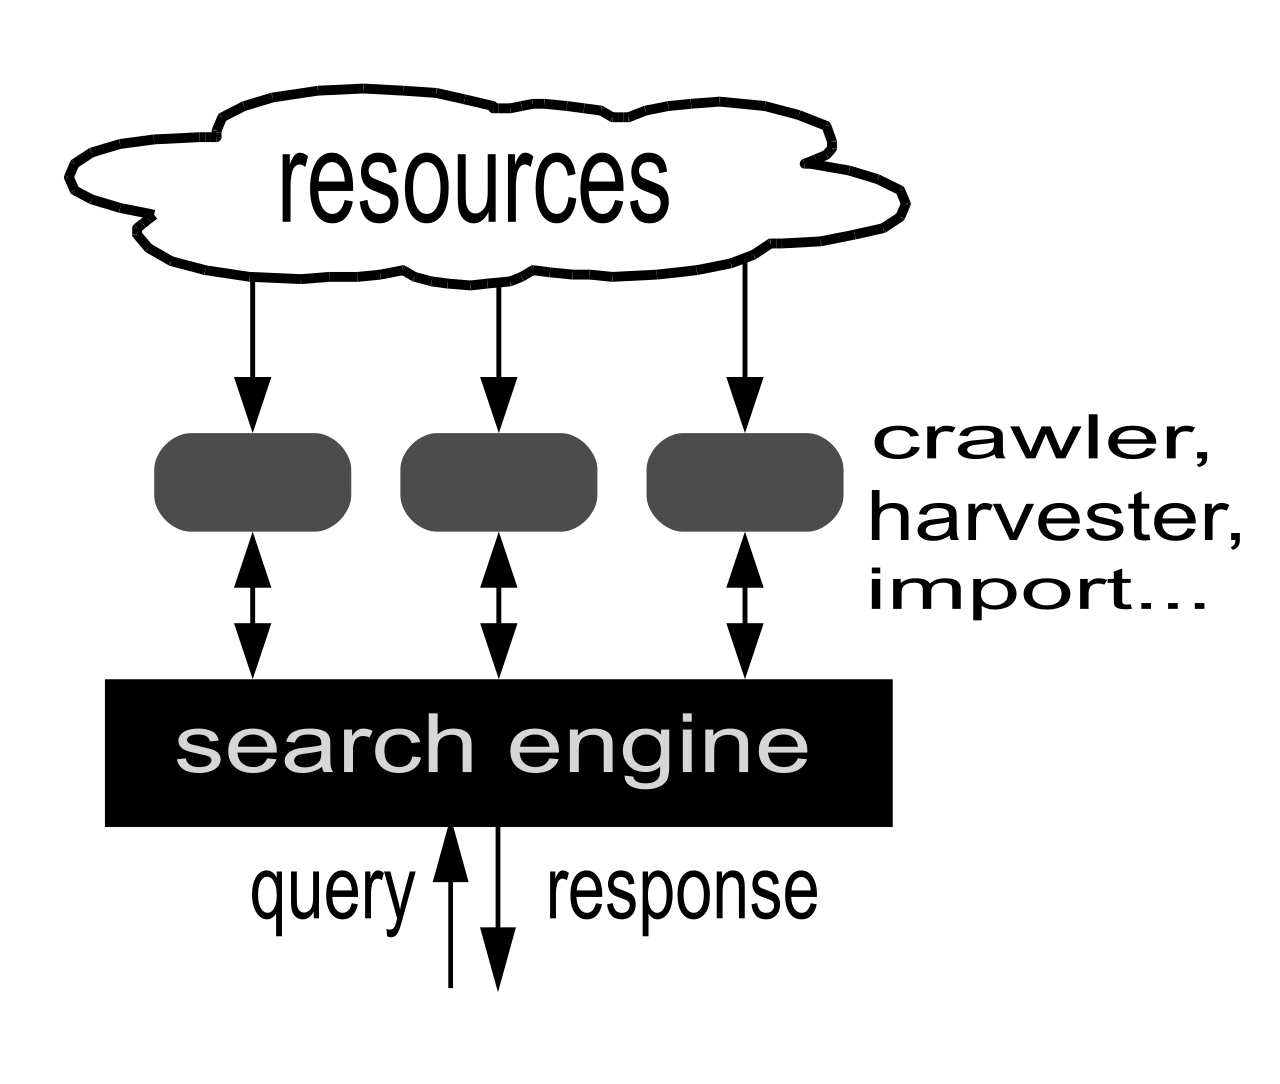
\includegraphics[width=0.66\linewidth]{assets/images/nestrukturovana-data/search-engine-concept.png}
  \caption[Koncept vyhledávače]{Zjednodušený koncept vyhledávače. Popis obrázku: crawler nebo harvester
  získává zdroje, vyhledávač nad nimi vytváří index a uživatel posílá dotaz, na který systém vrací odpověď
  nebo seřazené výsledky. Zdroj obrázku: Jakob Voss,
  \href{https://commons.wikimedia.org/wiki/File:Search-engine-diagram-en.svg}{Wikimedia Commons}, licence
  CC BY-SA 4.0.}
  \label{fig:q17-search-engine}
\end{figure}

\subsection*{Typy dotazů}

V IR se používají různé typy dotazů:
\begin{itemize}
    \item \textbf{keyword query} -- dotaz tvořený klíčovým slovem;
    \item \textbf{boolean query} -- dotaz pomocí AND, OR, NOT;
    \item \textbf{phrase query} -- přesná fráze, například \texttt{"data mining"};
    \item \textbf{proximity query} -- slova musí být blízko sebe;
    \item \textbf{full document query} -- dotazem je celý dokument;
    \item \textbf{natural language question} -- dotaz ve formě přirozené otázky.
\end{itemize}

Příklad:
\[
\texttt{cat AND dog}
\]
vrátí dokumenty obsahující oba termy.

\[
\texttt{cat AND NOT dog}
\]
vrátí dokumenty s termem \texttt{cat}, ale bez termu \texttt{dog}.

\subsection*{Předzpracování dokumentů pro vyhledávání}

Před vytvořením indexu se dokumenty obvykle převádějí do vhodné reprezentace.

Typický postup:
\begin{enumerate}
    \item získání dokumentů,
    \item extrakce textu z HTML, PDF, Wordu nebo skenů,
    \item OCR u skenovaných dokumentů,
    \item tokenizace,
    \item normalizace velikosti písmen,
    \item odstranění interpunkce nebo šumu,
    \item odstranění stop slov,
    \item stemming nebo lemmatizace,
    \item vytvoření termů, n-gramů nebo embeddingů,
    \item vytvoření indexu.
\end{enumerate}

\paragraph{Stop slova.}
Stop slova jsou častá slova s nízkou informační hodnotou, například \uv{a}, \uv{the}, \uv{of}.
Jejich odstranění může zmenšit index, ale u některých dotazů může škodit.

\paragraph{Stemming vs. lemmatizace.}
Stemming hrubě zkracuje slovo na kmen:
\[
\text{running},\ \text{runner},\ \text{runs}
\rightarrow
\text{run}.
\]

Lemmatizace převádí slovo na slovníkový tvar:
\[
\text{šel},\ \text{šla},\ \text{šli}
\rightarrow
\text{jít}.
\]

U češtiny je kvůli bohaté morfologii často vhodnější lemmatizace než jednoduchý stemming.

\subsection*{Document-term matice}

Po tokenizaci lze kolekci dokumentů reprezentovat jako document-term matici:
\[
X=(x_{ij}),
\]
kde:
\begin{itemize}
    \item řádky odpovídají dokumentům,
    \item sloupce termům,
    \item $x_{ij}$ je váha termu $j$ v dokumentu $i$.
\end{itemize}

Jednoduchá hodnota:
\[
x_{ij}=f_{ij},
\]
kde $f_{ij}$ je počet výskytů termu $j$ v dokumentu $i$.

\subsection*{Inverted index}

Pro rychlé vyhledávání se nepoužívá přímo celá document-term matice, ale \textbf{inverted index}.

Inverted index ukládá pro každý term seznam dokumentů, ve kterých se term vyskytuje:
\[
\text{term}
\rightarrow
\{(docID, frequency, positions)\}.
\]

Příklad:
\[
\texttt{cat}
\rightarrow
\{(d_1,2,[3,17]),(d_4,1,[8]),(d_9,5,[1,6,9,13,20])\}.
\]

Výhody:
\begin{itemize}
    \item rychlé vyhledávání dokumentů obsahujících term,
    \item možnost počítat skóre relevance,
    \item možnost podporovat frázové a proximity dotazy pomocí pozic termů.
\end{itemize}

\paragraph{Proč je index obrácený.}
Přímá reprezentace říká \uv{dokument $\rightarrow$ termy}. Vyhledávání ale typicky začíná termem v dotazu,
proto je efektivnější mít mapování \uv{term $\rightarrow$ dokumenty}. U velkých kolekcí se navíc posting listy
komprimují a při booleovském dotazu se nad nimi počítají průniky, sjednocení nebo rozdíly.

\subsection*{Booleovský model vyhledávání}

Booleovský model reprezentuje dokumenty jako množiny termů. Dotaz je logický výraz.

Operátory:
\[
AND,\quad OR,\quad NOT.
\]

Dokument je buď relevantní, nebo nerelevantní:
\[
rel(d,q)\in\{0,1\}.
\]

Výhody:
\begin{itemize}
    \item jednoduchý,
    \item přesný pro formální dotazy,
    \item dobře srozumitelný pro experty.
\end{itemize}

Nevýhody:
\begin{itemize}
    \item nepracuje dobře se stupněm relevance,
    \item neumí přirozeně řadit výsledky,
    \item nebere v úvahu frekvenci termů,
    \item AND může být příliš přísné a OR příliš široké.
\end{itemize}

\subsection*{Vektorový model vyhledávání}

Vektorový model reprezentuje dokument i dotaz jako vektory v prostoru termů:
\[
d_i=(w_{i1},w_{i2},\ldots,w_{ip}),
\]
\[
q=(w_{q1},w_{q2},\ldots,w_{qp}).
\]

Relevance dokumentu k dotazu se měří podobností vektorů. Nejčastěji kosinovou podobností:
\[
\cos(d_i,q)
=
\frac{d_i^\top q}
{\|d_i\|\|q\|}.
\]

Výsledek:
\begin{itemize}
    \item dokumenty nejsou jen relevantní/nerelevantní,
    \item dokumenty lze seřadit podle podobnosti s dotazem,
    \item model přirozeně využívá váhy termů.
\end{itemize}

\subsection*{TF-IDF}

TF-IDF je klasická váha termu v dokumentu. Kombinuje:
\begin{itemize}
    \item \textbf{TF} -- term frequency, tedy četnost termu v dokumentu;
    \item \textbf{IDF} -- inverse document frequency, tedy vzácnost termu v celé kolekci.
\end{itemize}

Term frequency:
\[
tf_{ij}=f_{ij}.
\]

Document frequency:
\[
df_j
=
|\{d_i:t_j\in d_i\}|.
\]

Inverse document frequency:
\[
idf_j
=
\log\left(\frac{N}{df_j}\right),
\]
kde $N$ je počet dokumentů v kolekci.

TF-IDF:
\[
w_{ij}
=
tf_{ij}\cdot idf_j.
\]

\paragraph{Intuice.}
Term je důležitý, pokud se často vyskytuje v daném dokumentu, ale není běžný ve všech dokumentech.

Slovo jako \uv{the} má vysokou četnost, ale nízké IDF. Specializovaný term může mít vysoké IDF.

\subsection*{BM25}

BM25 je modernější pravděpodobnostní skórovací funkce často používaná ve vyhledávačích.

Pro dotaz $q$ a dokument $d$:
\[
\begin{aligned}
score(d,q)
&=
\sum_{t\in q}
idf(t)
\frac{
f(t,d)(k_1+1)
}{
f(t,d)+k_1\left(1-b+b\frac{|d|}{avgdl}\right)
}.
\end{aligned}
\]

Kde:
\begin{itemize}
    \item $f(t,d)$ je četnost termu $t$ v dokumentu $d$,
    \item $|d|$ je délka dokumentu,
    \item $avgdl$ je průměrná délka dokumentu,
    \item $k_1$ a $b$ jsou laditelné parametry.
\end{itemize}

BM25 řeší například to, že dlouhé dokumenty mají přirozeně více výskytů slov.

\subsection*{Sparse a dense retrieval}

\subsubsection*{Sparse retrieval}

Sparse retrieval používá řídké vektory délky slovníku. Typicky:
\[
TF,\quad TF\text{-}IDF,\quad BM25.
\]

Výhody:
\begin{itemize}
    \item rychlé,
    \item dobře interpretovatelné,
    \item přesné pro klíčová slova.
\end{itemize}

Nevýhody:
\begin{itemize}
    \item hůře zachycuje synonymii,
    \item dokument bez přesného termu se nemusí najít,
    \item omezeně pracuje s významem.
\end{itemize}

\subsubsection*{Dense retrieval}

Dense retrieval používá husté embeddingové vektory:
\[
d_i \mapsto \mathbf{e}_{d_i}\in\mathbb{R}^k,
\qquad
q \mapsto \mathbf{e}_q\in\mathbb{R}^k.
\]

Podobnost:
\[
\cos(\mathbf{e}_{d_i},\mathbf{e}_q)
=
\frac{\mathbf{e}_{d_i}^{\top}\mathbf{e}_q}
{\|\mathbf{e}_{d_i}\|\|\mathbf{e}_q\|}.
\]

Výhody:
\begin{itemize}
    \item lepší zachycení významové podobnosti,
    \item vhodné pro sémantické vyhledávání,
    \item dokáže najít dokument i bez přesné shody slov.
\end{itemize}

Nevýhody:
\begin{itemize}
    \item horší interpretovatelnost,
    \item dražší výpočet,
    \item riziko nerelevantních, ale významově blízkých výsledků.
\end{itemize}

\subsubsection*{Hybridní retrieval}

V praxi se často kombinuje sparse a dense retrieval. Sparse část dobře zachytí přesná klíčová slova,
identifikátory a názvy, dense část pomůže se synonymy a významově podobnými formulacemi. Výsledky lze sloučit
například přes vážené skóre nebo re-ranking.

\subsection*{Hodnocení vyhledávání}

Pro vyhledávání a extrakci se používají metriky:

\[
Precision
=
\frac{TP}{TP+FP}.
\]

\[
Recall
=
\frac{TP}{TP+FN}.
\]

\[
F_1
=
2\frac{Precision\cdot Recall}{Precision+Recall}.
\]

Kde:
\begin{itemize}
    \item $TP$ jsou správně nalezené relevantní dokumenty,
    \item $FP$ jsou nalezené, ale nerelevantní dokumenty,
    \item $FN$ jsou relevantní dokumenty, které systém nenašel.
\end{itemize}

\begin{figure}[htbp]
  \centering
  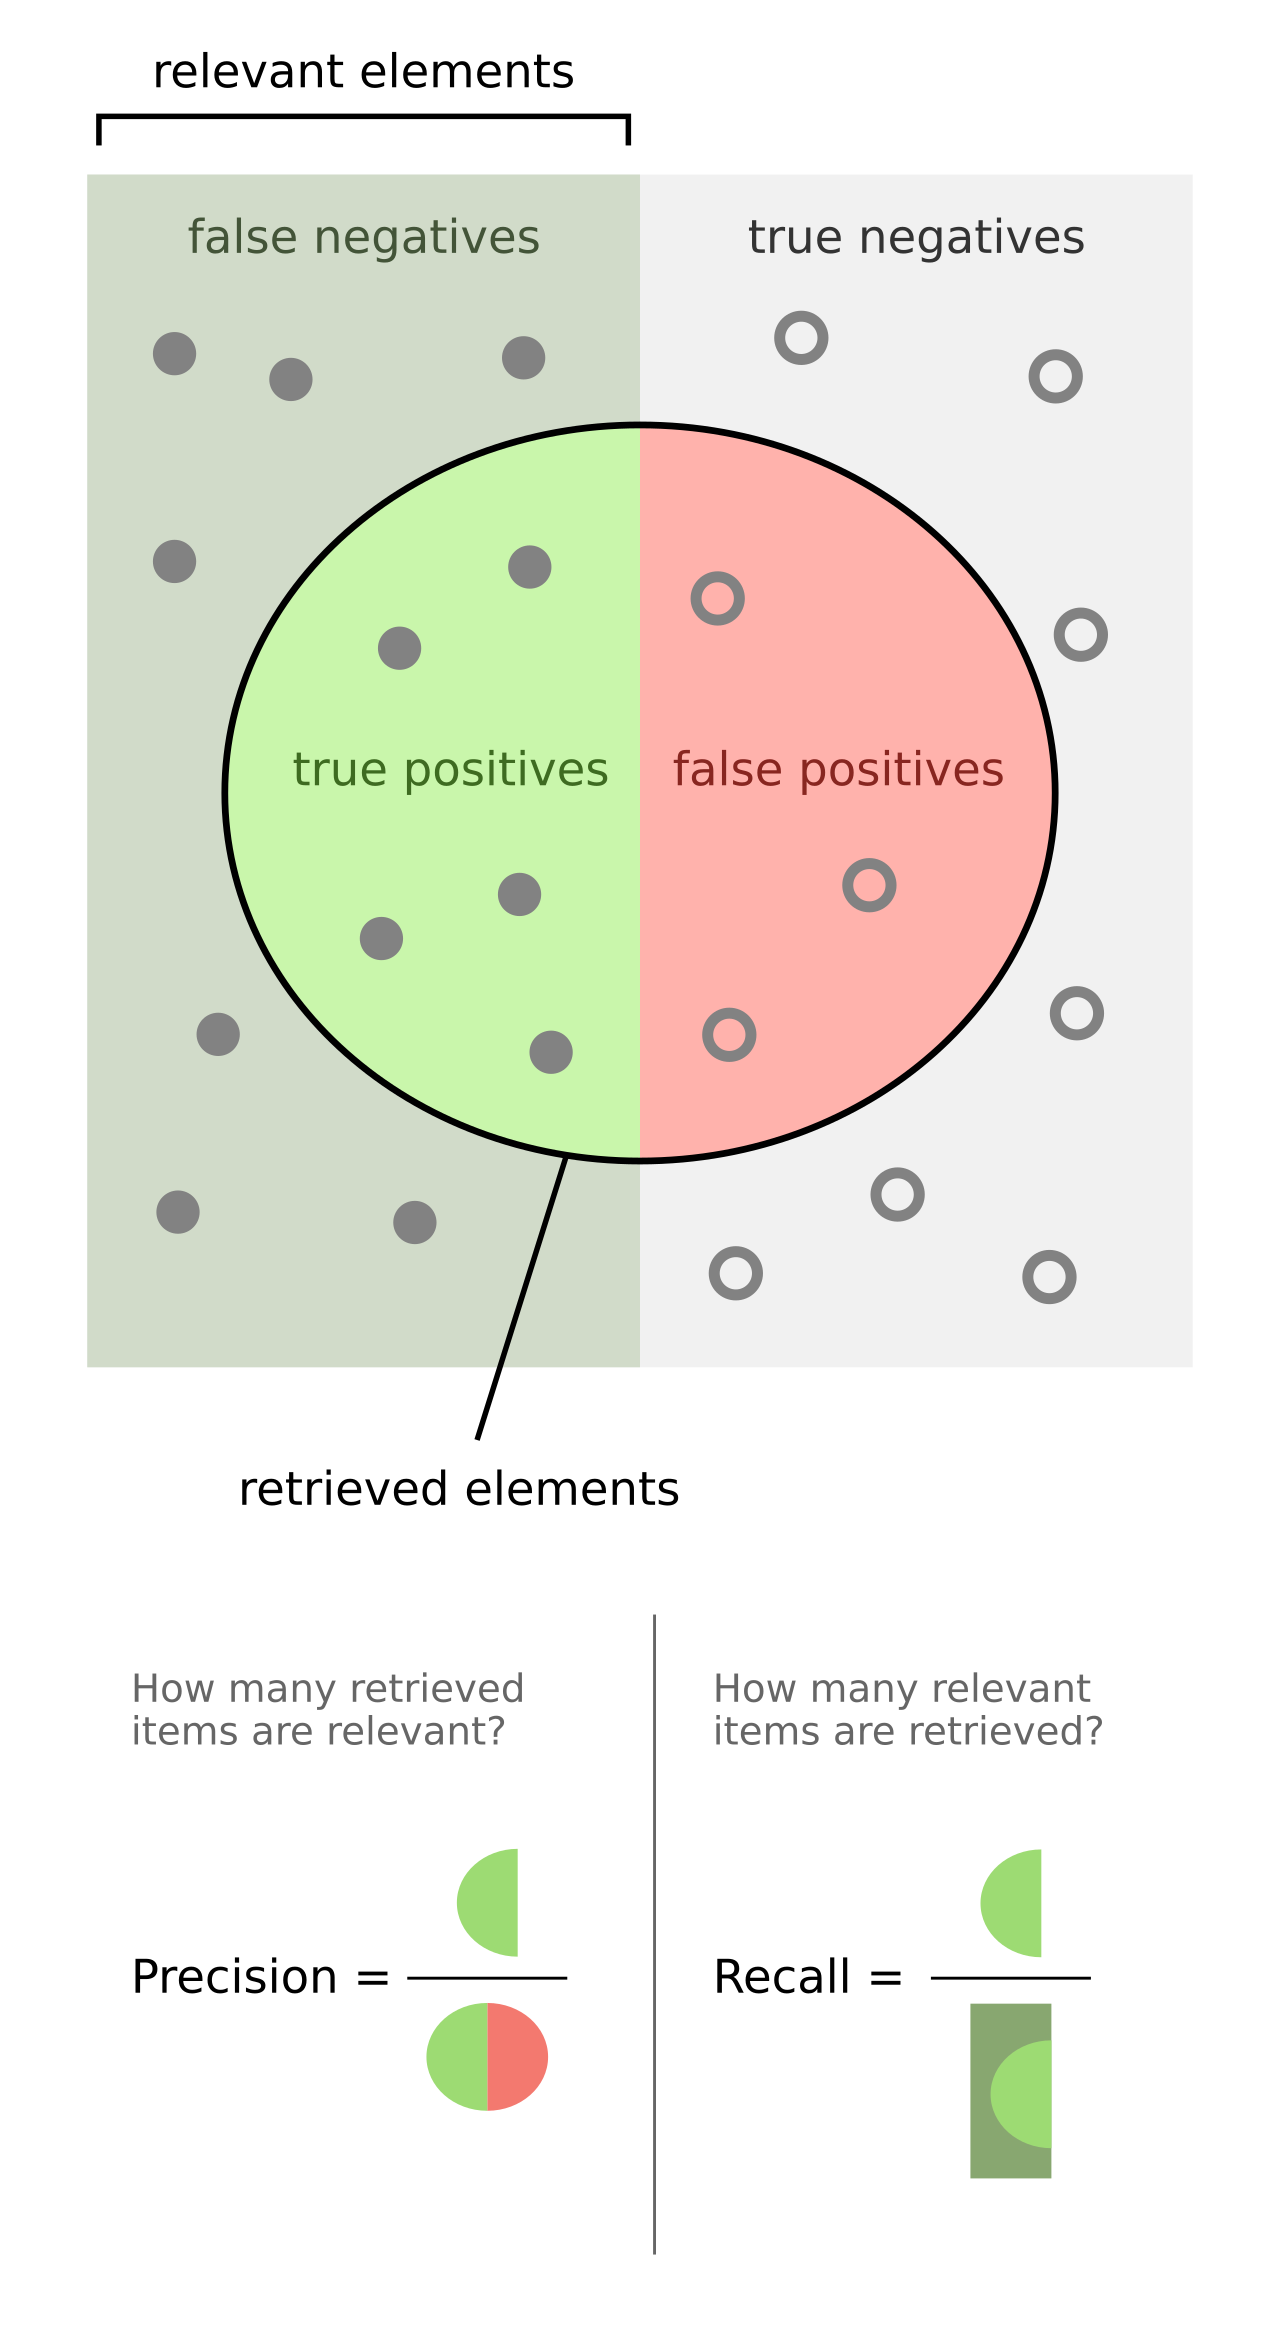
\includegraphics[width=0.56\linewidth]{assets/images/nestrukturovana-data/precision-recall.png}
  \caption[Precision a recall]{Vztah mezi precision a recall. Popis obrázku: relevantní prvky tvoří jednu
  množinu, nalezené prvky druhou; jejich průnik jsou true positives, nalezené nerelevantní prvky jsou false
  positives a nenalezené relevantní prvky jsou false negatives. Zdroj obrázku: Walber,
  \href{https://commons.wikimedia.org/wiki/File:Precisionrecall.svg}{Wikimedia Commons}, licence CC BY-SA 4.0.}
  \label{fig:q17-precision-recall}
\end{figure}

\paragraph{Napětí mezi precision a recall.}
Širší dotaz často zvýší recall, ale sníží precision. Užší dotaz může zvýšit precision, ale snížit recall.

\paragraph{Poznámka k IR.}
V reálném webovém vyhledávání často neznáme všechny relevantní dokumenty, takže recall se měří obtížně.
Snáze se obvykle odhaduje precision na vrácených výsledcích.

\subsection*{Extrakce informací}

Extrakce informací, Information Extraction, převádí nestrukturovaný nebo semistrukturovaný text na
strukturovaná data.

Obecně:
\[
\text{text}
\rightarrow
\text{tabulka / databáze / znalostní graf}.
\]

Na rozdíl od Information Retrieval, kde často stačí najít relevantní dokument, se Information Extraction snaží
vytáhnout konkrétní fakta. Výstup má být dále strojově použitelný: záznam v tabulce, JSON objekt, trojice ve
znalostním grafu nebo vyplněná šablona.

Příklad:
\begin{quote}
\uv{Oliver Blume, CEO of Volkswagen, announced sales growth of 23 MEUR in 2025.}
\end{quote}

Možný strukturovaný výstup:
\[
\begin{array}{lll}
\text{entity} & \text{type} & \text{value}\\
\hline
\text{Oliver Blume} & \text{PERSON} & -\\
\text{Volkswagen} & \text{ORGANIZATION} & -\\
\text{23 MEUR} & \text{MONEY} & 23\\
\text{2025} & \text{DATE} & 2025
\end{array}
\]

A vztah:
\[
CEO\_of(\text{Oliver Blume},\text{Volkswagen}).
\]

\subsection*{Named Entity Recognition}

Named Entity Recognition, NER, hledá pojmenované entity v textu a přiřazuje jim typ.

Typické typy:
\begin{itemize}
    \item osoby,
    \item organizace,
    \item lokace a geopolitické entity,
    \item datumy,
    \item měnové částky,
    \item produkty,
    \item události,
    \item doménově specifické entity.
\end{itemize}

Přístupy k NER:
\begin{itemize}
    \item \textbf{regulární výrazy} -- vhodné pro formální entity, například částky nebo data;
    \item \textbf{gazetteery} -- slovníky známých entit;
    \item \textbf{ručně psaná pravidla} -- využívají kontext, tvar slov a gramatiku;
    \item \textbf{statistické modely} -- například CRF;
    \item \textbf{transformerové modely a LLM} -- dnes velmi silné pro mnoho jazyků a domén.
\end{itemize}

\paragraph{Problém gazetteerů.}
Slovník entit může říct, že \uv{Denver} je město, ale v konkrétním textu může jít o osobu. Naopak nová firma
nebo produkt ještě ve slovníku nemusí být.

\subsection*{Entity linking}

Entity linking nejde jen po typu entity, ale po konkrétní entitě ve znalostní bázi:
\[
\text{\uv{Paris}}
\rightarrow
\text{Paris, France}
\quad
\text{nebo}
\quad
\text{Paris Hilton}.
\]

Postup:
\begin{enumerate}
    \item rozpoznat kandidátní entitu v textu,
    \item najít kandidáty ve znalostní bázi,
    \item vybrat správnou entitu podle kontextu,
    \item propojit text s identifikátorem ve znalostním grafu.
\end{enumerate}

Příklady znalostních bází:
\begin{itemize}
    \item Wikidata,
    \item DBpedia,
    \item YAGO,
    \item interní firemní znalostní graf.
\end{itemize}

\subsection*{Relation extraction}

Relation extraction hledá vztahy mezi entitami:
\[
relation(entity_1,entity_2).
\]

Příklady:
\[
works\_for(\text{person},\text{organization}),
\]
\[
located\_in(\text{company},\text{country}),
\]
\[
acquired(\text{company}_1,\text{company}_2).
\]

Přístupy:
\begin{itemize}
    \item pravidla a vzory,
    \item dependency parsing,
    \item supervised learning,
    \item distant supervision,
    \item transformerové modely,
    \item LLM s kontrolou výstupu.
\end{itemize}

\subsection*{Web scraping}

Web scraping je automatizované získávání dat z webových stránek. Cílem je převést webový obsah na
strukturovaná data:
\[
HTML
\rightarrow
\text{tabulka / JSON / databáze}.
\]

\begin{figure}[htbp]
  \centering
  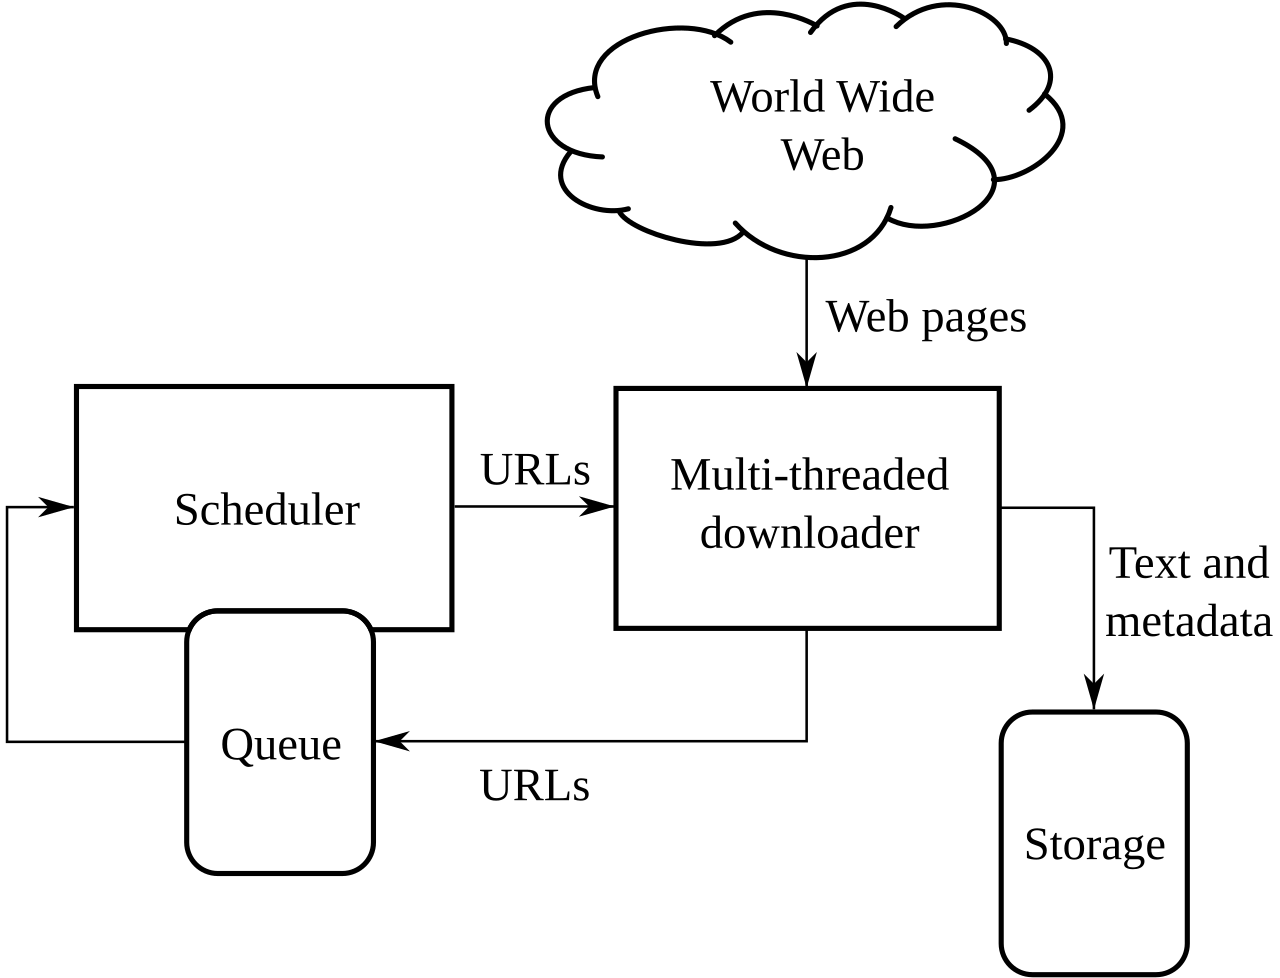
\includegraphics[width=0.86\linewidth]{assets/images/nestrukturovana-data/web-crawler-architecture.png}
  \caption[Architektura webového crawleru]{Základní architektura webového crawleru. Popis obrázku: scheduler
  spravuje frontu URL, downloader stahuje webové stránky a z textu, metadat a odkazů se doplňuje další obsah
  nebo nové URL do fronty. Zdroj obrázku: dnet podle ChaTo,
  \href{https://commons.wikimedia.org/wiki/File:WebCrawlerArchitecture.svg}{Wikimedia Commons}, licence
  CC BY-SA 3.0.}
  \label{fig:q17-web-crawler}
\end{figure}

\paragraph{Crawler vs. scraper.}
Crawler systematicky prochází odkazy a objevuje stránky. Scraper z konkrétních stránek extrahuje požadované
položky. V praxi se oba kroky často kombinují: crawler najde stránky a scraper z nich vytáhne strukturovaná
data.

\subsection*{API vs. scraping}

\begin{itemize}
    \item \textbf{API} poskytuje data ve strukturované podobě, typicky JSON nebo XML.
    Je stabilnější a vhodnější, pokud existuje.
    
    \item \textbf{Scraping} získává data přímo z HTML stránky. Je křehčí, protože změna vzhledu stránky může
    rozbít extrakční pravidla.
\end{itemize}

Obecně:
\[
\text{API} > \text{scraping},
\]
pokud API poskytuje potřebná data, je dostupné a jeho podmínky umožňují použití.

\subsection*{Typický postup web scrapingu}

\begin{enumerate}
    \item definovat cíl a datové položky,
    \item ověřit dostupnost API,
    \item zkontrolovat podmínky použití webu,
    \item stáhnout stránku přes HTTP požadavek,
    \item naparsovat HTML do DOM stromu,
    \item vybrat prvky pomocí CSS selektorů nebo XPath,
    \item zpracovat paginaci nebo odkazy,
    \item vyčistit a normalizovat data,
    \item uložit výstup do CSV, JSON, databáze nebo datového skladu,
    \item monitorovat změny struktury webu.
\end{enumerate}

HTTP požadavek:
\[
GET\ /products?page=1
\]

Výstup:
\[
\texttt{status code},\quad \texttt{headers},\quad \texttt{body}.
\]

\subsection*{CSS selektory a XPath}

CSS selektor:
\[
\texttt{div.product span.price}
\]

XPath:
\[
\texttt{//div[@class='product']//span[@class='price']}
\]

CSS selektory bývají jednodušší, XPath je expresivnější pro složitější stromové dotazy.

\subsection*{Dynamické weby}

Mnoho webů načítá obsah pomocí JavaScriptu. Pak jednoduché stažení HTML nemusí stačit.

Možnosti:
\begin{itemize}
    \item najít síťový API požadavek v prohlížeči,
    \item použít headless browser,
    \item použít Selenium nebo Playwright,
    \item počkat na vykreslení stránky,
    \item zpracovat infinite scroll.
\end{itemize}

\subsection*{Wrapper generation}

Wrapper je extrakční pravidlo nebo program, který z daného typu stránky vytahuje požadovaná data.

Příklad:
\[
\text{produktová stránka}
\rightarrow
\{\text{název},\text{cena},\text{dostupnost},\text{hodnocení}\}.
\]

Wrapper může být:
\begin{itemize}
    \item ručně napsaný,
    \item interaktivně vytvořený klikáním na prvky ve stránce,
    \item částečně automaticky naučený z příkladů.
\end{itemize}

Výhoda wrapperu:
\begin{itemize}
    \item vysoká přesnost pro konkrétní web.
\end{itemize}

Nevýhoda:
\begin{itemize}
    \item křehkost při změně šablony webu.
\end{itemize}

\subsection*{Právní a etické aspekty scrapingu}

Při scrapingu je nutné řešit:
\begin{itemize}
    \item podmínky použití webu,
    \item soubor \texttt{robots.txt},
    \item autorská práva a databázová práva,
    \item ochranu osobních údajů,
    \item zákaz obcházení technických omezení,
    \item přiměřenou zátěž serveru,
    \item transparentnost účelu sběru dat.
\end{itemize}

\paragraph{Robots.txt.}
Soubor \texttt{robots.txt} říká crawlerům, které části webu nemají navštěvovat. Není to totéž co právní
smlouva, ale je to důležitá technická a etická konvence.

\paragraph{Rate limiting.}
Slušný scraper omezuje frekvenci požadavků, používá cache, identifikuje se rozumným user-agentem a respektuje
chyby serveru. Technicky funkční scraping ještě neznamená, že je vhodný právně, eticky nebo provozně.

\paragraph{Osobní údaje.}
Pokud scraping získává osobní údaje, je nutné mít právní titul zpracování, minimalizovat rozsah dat,
zajistit bezpečné uložení a respektovat práva subjektů údajů.

\subsection*{Nástroje}

Pro praktickou práci se používají například:
\begin{itemize}
    \item \textbf{Python:} \texttt{requests}, \texttt{BeautifulSoup}, \texttt{lxml}, \texttt{Scrapy},
    \texttt{Selenium}, \texttt{Playwright}, \texttt{pandas};
    \item \textbf{IR a vyhledávání:} Apache Lucene, Elasticsearch, OpenSearch, Solr;
    \item \textbf{NLP/IE:} spaCy, NLTK, Stanza, UDPipe, transformers;
    \item \textbf{datové formáty:} JSON, XML, CSV, Parquet;
    \item \textbf{uložení:} relační databáze, dokumentové databáze, datové sklady, knowledge graphs.
\end{itemize}

\subsection*{Shrnutí ke zkoušce}

Nestrukturovaná a semistrukturovaná data vyžadují převod do strojově zpracovatelné podoby. Semistrukturovaná
data jako XML, JSON a HTML mají stromovou nebo dokumentovou strukturu. Nestrukturovaný text je třeba
tokenizovat, normalizovat a reprezentovat pomocí termů, vah nebo embeddingů.

Porovnávání vzorů zahrnuje regulární výrazy, edit distance a sémantickou podobnost. Vyhledávání dokumentů
využívá indexování, zejména inverted index. Booleovský model pracuje s přesnou logickou shodou, zatímco
vektorový model reprezentuje dotaz i dokument jako vektory a řadí výsledky podle podobnosti:
\[
\cos(d,q)=\frac{d^\top q}{\|d\|\|q\|}.
\]

Extrakce informací převádí text na strukturovaná data. Patří sem NER, entity linking, relation extraction a
template filling. Web scraping automatizovaně získává data z webových stránek, typicky přes HTTP, HTML DOM,
CSS selektory a XPath. Pokud existuje API, je obvykle vhodnější než scraping. Při scrapingu je nutné řešit
technická omezení, kvalitu dat, právní podmínky, etiku a ochranu osobních údajů.

\subsection*{Zdroje}

\begin{itemize}
    \item Manning, Raghavan, Schütze:
    \href{https://nlp.stanford.edu/IR-book/}{Introduction to Information Retrieval}.
    \item Python dokumentace:
    \href{https://docs.python.org/3/library/re.html}{\texttt{re} -- Regular expression operations}.
    \item MDN Web Docs:
    \href{https://developer.mozilla.org/en-US/docs/Web/API/Document\_Object\_Model}{Document Object Model}.
    \item RFC 9309:
    \href{https://www.rfc-editor.org/rfc/rfc9309}{Robots Exclusion Protocol}.
    \item Scrapy dokumentace:
    \href{https://docs.scrapy.org/en/latest/topics/selectors.html}{Selectors}.
    \item Wikimedia Commons:
    \href{https://commons.wikimedia.org/wiki/File:DOM\_Beispielbaum.svg}{DOM Beispielbaum}.
    \item Wikimedia Commons:
    \href{https://commons.wikimedia.org/wiki/File:Search-engine-diagram-en.svg}{Search-engine-diagram-en}.
    \item Wikimedia Commons:
    \href{https://commons.wikimedia.org/wiki/File:Precisionrecall.svg}{Precisionrecall}.
    \item Wikimedia Commons:
    \href{https://commons.wikimedia.org/wiki/File:WebCrawlerArchitecture.svg}{WebCrawlerArchitecture}.
\end{itemize}

\newpage

\section{Zpracování textových dat. Lingvistické zpracování přirozeného jazyka, jazykové modely, analytické metody, existující nástroje}

\subsection{Základní vymezení}

Zpracování textových dat se zabývá převodem textu do podoby, se kterou mohou pracovat analytické algoritmy.
Text jako takový je pro počítač pouze posloupnost znaků. Analytický model ale potřebuje příznaky:
\[
\text{text}
\rightarrow
\text{tokeny}
\rightarrow
\text{features / vectors}
\rightarrow
\text{model}.
\]

\textbf{Natural Language Processing} neboli NLP je oblast na pomezí lingvistiky, informatiky a umělé
inteligence, která se zabývá zpracováním přirozeného jazyka počítačem.

\textbf{Text analytics} lze chápat jako propojení NLP a datové analytiky nad texty. NLP často řeší jazykové
předzpracování a reprezentaci textu, zatímco text analytics se soustředí na získání analytického výstupu:
klasifikace, vyhledávání, sentiment, extrakce informací, sumarizace, topic modeling apod.

\paragraph{Příklad.}
Věta:
\begin{quote}
\uv{Zákazník si stěžoval na pomalé doručení.}
\end{quote}
může být převedena na:
\begin{itemize}
    \item tokeny: \texttt{Zákazník, si, stěžoval, na, pomalé, doručení};
    \item lemma: \texttt{zákazník, se, stěžovat, na, pomalý, doručení};
    \item sentiment: negativní;
    \item aspekt: doručení;
    \item entita: zákazník.
\end{itemize}

\subsection{Text není úplně bez struktury}

Text se často označuje jako nestrukturovaný, ale přirozený jazyk má mnoho vrstev:
\begin{itemize}
    \item znaky,
    \item morfémy,
    \item subword jednotky,
    \item slova,
    \item fráze,
    \item věty,
    \item odstavce,
    \item dokumenty.
\end{itemize}

Kromě toho má jazyk:
\begin{itemize}
    \item pravopis,
    \item gramatiku,
    \item morfologii,
    \item syntax,
    \item význam,
    \item pragmatiku a kontext.
\end{itemize}

\paragraph{Důležité pro češtinu.}
Čeština má bohatou morfologii a volnější slovosled než angličtina. Proto postupy vyvinuté pro angličtinu
nemusí bez úprav fungovat stejně dobře pro češtinu. U češtiny je důležitá hlavně kvalitní tokenizace,
lemmatizace a morfologické značkování.

\subsection{Obecný pipeline zpracování textu}

Typický postup:
\begin{enumerate}
    \item získání dokumentů,
    \item čištění textu,
    \item tokenizace,
    \item rozdělení na věty,
    \item normalizace,
    \item odstranění stop slov,
    \item stemming nebo lemmatizace,
    \item POS tagging a morfologická analýza,
    \item syntaktické zpracování,
    \item extrakce entit a vztahů,
    \item vytvoření číselné reprezentace,
    \item modelování a vyhodnocení.
\end{enumerate}

Ne všechny kroky jsou vždy potřeba. U moderních transformerových modelů se část jazykového zpracování učí
uvnitř modelu, ale porozumění těmto krokům je pořád důležité pro diagnostiku chyb a interpretaci výsledků.

\subsection{Čištění a normalizace textu}

Čištění textu zahrnuje:
\begin{itemize}
    \item odstranění HTML značek,
    \item odstranění boilerplate textu z webu,
    \item dekódování HTML entit,
    \item sjednocení kódování,
    \item odstranění duplicit,
    \item opravy typografických znaků,
    \item normalizaci mezer,
    \item zachování nebo odstranění interpunkce podle úlohy.
\end{itemize}

Normalizace může zahrnovat:
\begin{itemize}
    \item převod na malá písmena,
    \item normalizaci čísel,
    \item normalizaci URL adres,
    \item normalizaci uživatelských jmen,
    \item převod emotikonů,
    \item opravu překlepů.
\end{itemize}

\paragraph{Pozor.}
Převod na malá písmena může zhoršit NER, protože velká písmena pomáhají poznat jména osob, organizací a míst.

\subsection{Tokenizace}

Tokenizace rozděluje text na tokeny:
\[
\text{text}
\rightarrow
(t_1,t_2,\ldots,t_n).
\]

Token může být:
\begin{itemize}
    \item slovo,
    \item číslo,
    \item interpunkce,
    \item emotikon,
    \item subword jednotka,
    \item znak.
\end{itemize}

Příklad:
\begin{quote}
\uv{Prof. Novák přišel v 8:30.}
\end{quote}

Tokenizace není vždy triviální:
\begin{itemize}
    \item \texttt{Prof.} obsahuje tečku, ale nekončí větu,
    \item \texttt{8:30} je jeden časový údaj,
    \item \texttt{GPT-4} může být jeden token nebo více tokenů,
    \item emotikony a hashtagy mají speciální význam.
\end{itemize}

\paragraph{Subword tokenizace.}
Moderní jazykové modely často nepracují přímo se slovy, ale se subword jednotkami, například WordPiece, BPE
nebo unigram tokenizací. Výhoda je, že model umí zpracovat i neznámá nebo složená slova rozložením na části.
Nevýhoda je horší interpretovatelnost tokenů a rozdílná délka vstupu podle použitého tokenizeru.

\subsection{Rozdělení na věty}

Sentence splitting rozděluje text na věty. Problém je, že tečka nemusí vždy znamenat konec věty:
\begin{itemize}
    \item zkratky: \texttt{Prof.}, \texttt{Dr.}, \texttt{např.};
    \item desetinná čísla: \texttt{3.14};
    \item iniciály: \texttt{T. G. Masaryk};
    \item URL adresy.
\end{itemize}

Proto se používají pravidla nebo modely, které berou v úvahu kontext.

\subsection{Stop slova}

Stop slova jsou velmi častá slova, která často nenesou silný tematický význam:
\[
\text{a},\quad \text{the},\quad \text{of},\quad \text{se},\quad \text{v}.
\]

Odstranění stop slov může pomoci u:
\begin{itemize}
    \item vyhledávání,
    \item topic modelingu,
    \item klasických bag-of-words modelů.
\end{itemize}

Může ale škodit u:
\begin{itemize}
    \item sentimentu,
    \item negace,
    \item právních textů,
    \item jazykových modelů.
\end{itemize}

Například slovo \uv{ne} je krátké a časté, ale pro sentiment je zásadní:
\begin{center}
\uv{dobré} $\neq$ \uv{ne dobré}.
\end{center}

\subsection{Stemming a lemmatizace}

\subsubsection{Stemming}

Stemming převádí slova na hrubý kmen. Nemusí jít o skutečný slovníkový tvar.

Příklad v angličtině:
\[
\text{running},\ \text{runs},\ \text{runner}
\rightarrow
\text{run}.
\]

Výhody:
\begin{itemize}
    \item rychlý,
    \item jednoduchý,
    \item snižuje počet termů.
\end{itemize}

Nevýhody:
\begin{itemize}
    \item může produkovat neexistující tvary,
    \item může spojit významově odlišná slova,
    \item pro morfologicky bohaté jazyky může být příliš hrubý.
\end{itemize}

\subsubsection{Lemmatizace}

Lemmatizace převádí slova na lemma, tedy základní slovníkový tvar.

Příklad v češtině:
\begin{center}
\uv{šel}, \uv{šla}, \uv{šli} $\rightarrow$ \uv{jít}.
\end{center}

\begin{center}
\uv{dobrý}, \uv{dobrá}, \uv{dobré} $\rightarrow$ \uv{dobrý}.
\end{center}

Výhody:
\begin{itemize}
    \item lingvisticky přesnější,
    \item vhodná pro češtinu,
    \item zlepšuje spojení různých tvarů stejného slova.
\end{itemize}

Nevýhody:
\begin{itemize}
    \item pomalejší,
    \item vyžaduje jazykové nástroje,
    \item u neznámých slov může chybovat.
\end{itemize}

\subsection{POS tagging a morfologická analýza}

POS tagging přiřazuje slovům slovní druh:
\[
token
\rightarrow
\text{noun, verb, adjective, adverb, ...}
\]

Morfologická analýza přidává další znaky, například:
\begin{itemize}
    \item pád,
    \item číslo,
    \item rod,
    \item čas,
    \item osoba,
    \item stupeň.
\end{itemize}

Příklad:
\begin{center}
\uv{kočky}
\end{center}
může být:
\begin{itemize}
    \item 1. pád množného čísla,
    \item 2. pád jednotného čísla.
\end{itemize}

Správná interpretace často závisí na kontextu.

\subsection{Syntaktické zpracování}

Syntaktické zpracování analyzuje strukturu věty.

\subsubsection{Shallow parsing / chunking}

Chunking hledá fráze, například jmenné fráze:
\begin{center}
\uv{velmi dobrý fotoaparát} $\rightarrow$ noun phrase.
\end{center}

\subsubsection{Full syntactic parsing}

Full parsing vytváří úplnější syntaktickou strukturu věty. Často se používá dependency parsing, který
určuje vztahy mezi slovy:
\[
\text{subject},\quad \text{object},\quad \text{modifier},\quad \text{case},\quad \text{compound}.
\]

Příklad:
\begin{quote}
\uv{Zákazník koupil telefon.}
\end{quote}

Vztahy:
\[
\operatorname{subject}(koupil,zakaznik),
\qquad
\operatorname{object}(koupil,telefon).
\]

Použití:
\begin{itemize}
    \item relation extraction,
    \item sentiment k aspektům,
    \item detekce subjektu a objektu,
    \item extrakce událostí.
\end{itemize}

\begin{figure}[htbp]
  \centering
  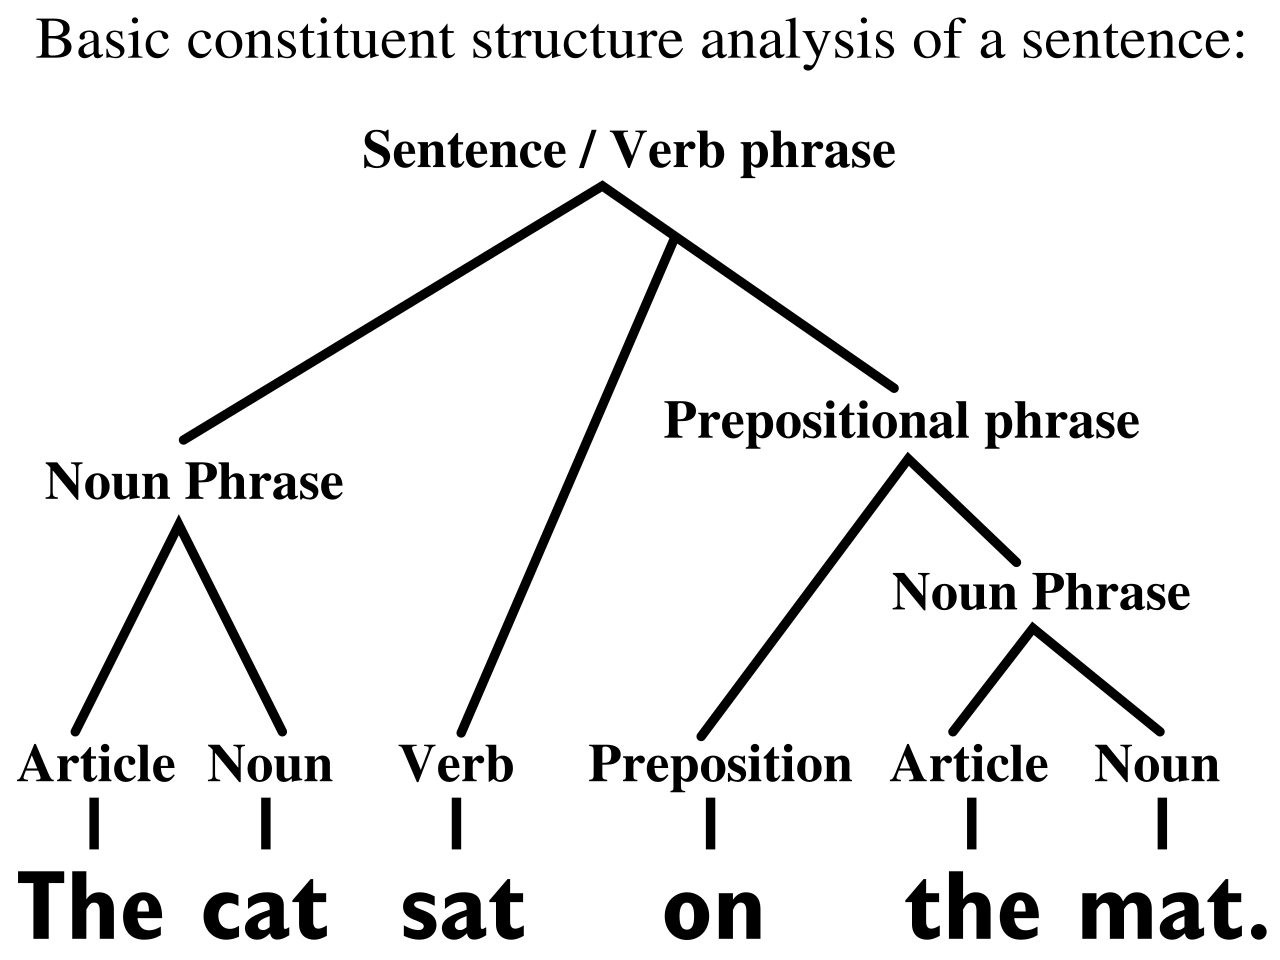
\includegraphics[width=0.82\linewidth]{assets/images/zpracovani-textovych-dat/syntax-tree.png}
  \caption[Syntaktický strom věty]{Příklad konstituentního syntaktického stromu. Popis obrázku: věta je
  rozložena na jmennou frázi, slovesnou část a předložkovou frázi; strom ukazuje hierarchii částí věty,
  kterou lze využít při parsingu nebo extrakci vztahů. Zdroj obrázku: AnonMoos,
  \href{https://commons.wikimedia.org/wiki/File:Basic\_constituent\_structure\_analysis\_English\_sentence.svg}{Wikimedia
  Commons}, public domain.}
  \label{fig:q18-syntax-tree}
\end{figure}

\subsection{Coreference resolution}

Coreference resolution řeší, které výrazy odkazují na stejnou entitu.

Příklad:
\begin{quote}
\uv{Koupil jsem telefon Samsung. Je velmi rychlý.}
\end{quote}

Zájmeno \uv{Je} odkazuje na:
\[
\text{telefon Samsung}.
\]

Coreference je důležitá pro:
\begin{itemize}
    \item extrakci informací,
    \item sumarizaci,
    \item sentiment,
    \item otázky a odpovědi.
\end{itemize}

\subsection{Reprezentace textu pro modely}

Algoritmy obvykle neumějí pracovat přímo s textem. Potřebují číselnou reprezentaci:
\[
\text{text}
\rightarrow
\mathbf{x}\in\mathbb{R}^p.
\]

Základní přístupy:
\begin{itemize}
    \item bag-of-words,
    \item n-gramy,
    \item TF-IDF,
    \item topic modely,
    \item word embeddings,
    \item contextual embeddings,
    \item sentence embeddings.
\end{itemize}

\subsection{Bag-of-words}

Bag-of-words reprezentuje dokument podle výskytu slov bez ohledu na jejich pořadí.

Dokument:
\[
d_i=(w_{i1},w_{i2},\ldots,w_{ip}),
\]
kde $p$ je velikost slovníku.

Hodnota $w_{ij}$ může být:
\begin{itemize}
    \item binární výskyt,
    \item četnost termu,
    \item TF-IDF váha.
\end{itemize}

Výhody:
\begin{itemize}
    \item jednoduché,
    \item dobře použitelné s klasickými ML modely,
    \item interpretovatelné.
\end{itemize}

Nevýhody:
\begin{itemize}
    \item ztrácí pořadí slov,
    \item nezachycuje význam,
    \item má vysokou dimenzi,
    \item nezvládá dobře synonymii a polysémii.
\end{itemize}

\subsection{N-gramy}

N-gram je posloupnost $n$ tokenů:
\[
(w_t,w_{t+1},\ldots,w_{t+n-1}).
\]

Příklady:
\begin{itemize}
    \item unigram: \texttt{data},
    \item bigram: \texttt{data mining},
    \item trigram: \texttt{natural language processing}.
\end{itemize}

N-gramy zachytí část lokálního pořadí slov. Jsou užitečné například pro:
\begin{itemize}
    \item klasifikaci textů,
    \item jazykové modely,
    \item vyhledávání frází,
    \item detekci ustálených spojení.
\end{itemize}

Nevýhoda:
\begin{itemize}
    \item velikost slovníku rychle roste s $n$.
\end{itemize}

\subsection{TF-IDF reprezentace}

TF-IDF váha:
\[
w_{ij}
=
tf_{ij}\cdot idf_j.
\]

Kde:
\[
idf_j=
\log\left(\frac{N}{df_j}\right).
\]

TF-IDF zvýrazňuje slova, která jsou častá v daném dokumentu, ale vzácná v celé kolekci.

Použití:
\begin{itemize}
    \item vyhledávání,
    \item klasifikace dokumentů,
    \item clustering dokumentů,
    \item podobnost dokumentů.
\end{itemize}

Kosinová podobnost:
\[
\cos(d_i,d_j)
=
\frac{d_i^\top d_j}
{\|d_i\|\|d_j\|}.
\]

\subsection{Klasické jazykové modely}

Jazykový model přiřazuje pravděpodobnost posloupnosti slov:
\[
P(w_1,w_2,\ldots,w_T).
\]

Pomocí řetězového pravidla:
\[
P(w_1,\ldots,w_T)
=
\prod_{t=1}^{T}
P(w_t|w_1,\ldots,w_{t-1}).
\]

Protože dlouhá historie je nepraktická, n-gramový model zjednodušuje:
\[
P(w_t|w_1,\ldots,w_{t-1})
\approx
P(w_t|w_{t-n+1},\ldots,w_{t-1}).
\]

Bigramový model:
\[
P(w_1,\ldots,w_T)
\approx
\prod_{t=1}^{T}
P(w_t|w_{t-1}).
\]

Problém:
\begin{itemize}
    \item mnoho n-gramů se ve vzorku nevyskytne,
    \item potřebujeme vyhlazování,
    \item model má omezený kontext,
    \item nepracuje dobře se synonymy ani s významem.
\end{itemize}

\subsection{Word embeddings}

Word embedding je vektorová reprezentace slova:
\[
w
\mapsto
\mathbf{e}_w\in\mathbb{R}^k.
\]

Na rozdíl od one-hot reprezentace je embedding:
\begin{itemize}
    \item hustý,
    \item nízkorozměrný,
    \item naučený z dat,
    \item schopný zachytit významovou podobnost.
\end{itemize}

One-hot reprezentace:
\[
\text{pes}=(0,0,1,0,\ldots,0).
\]

Embedding:
\[
\text{pes}\mapsto (0.12,-0.41,0.33,\ldots).
\]

Podobnost slov lze měřit kosinovou podobností:
\[
\cos(\mathbf{e}_a,\mathbf{e}_b)
=
\frac{\mathbf{e}_a^\top\mathbf{e}_b}
{\|\mathbf{e}_a\|\|\mathbf{e}_b\|}.
\]

\subsection{Distribuční hypotéza}

Embeddingy vycházejí z distribuční hypotézy:
\begin{center}
slova s podobným kontextem mají podobný význam.
\end{center}

Například slova \uv{pes} a \uv{kočka} se často vyskytují v podobných kontextech:
\begin{center}
\uv{krmit}, \uv{zvíře}, \uv{mazlíček}, \uv{veterinář}.
\end{center}

Proto by jejich vektory měly být blízko.

\subsection{Word2Vec}

Word2Vec je metoda pro učení slovních embeddingů pomocí jednoduché neuronové sítě.

Existují dvě základní varianty:
\begin{itemize}
    \item \textbf{CBOW} -- z kontextu predikuje prostřední slovo;
    \item \textbf{Skip-gram} -- z prostředního slova predikuje okolní slova.
\end{itemize}

\begin{figure}[htbp]
  \centering
  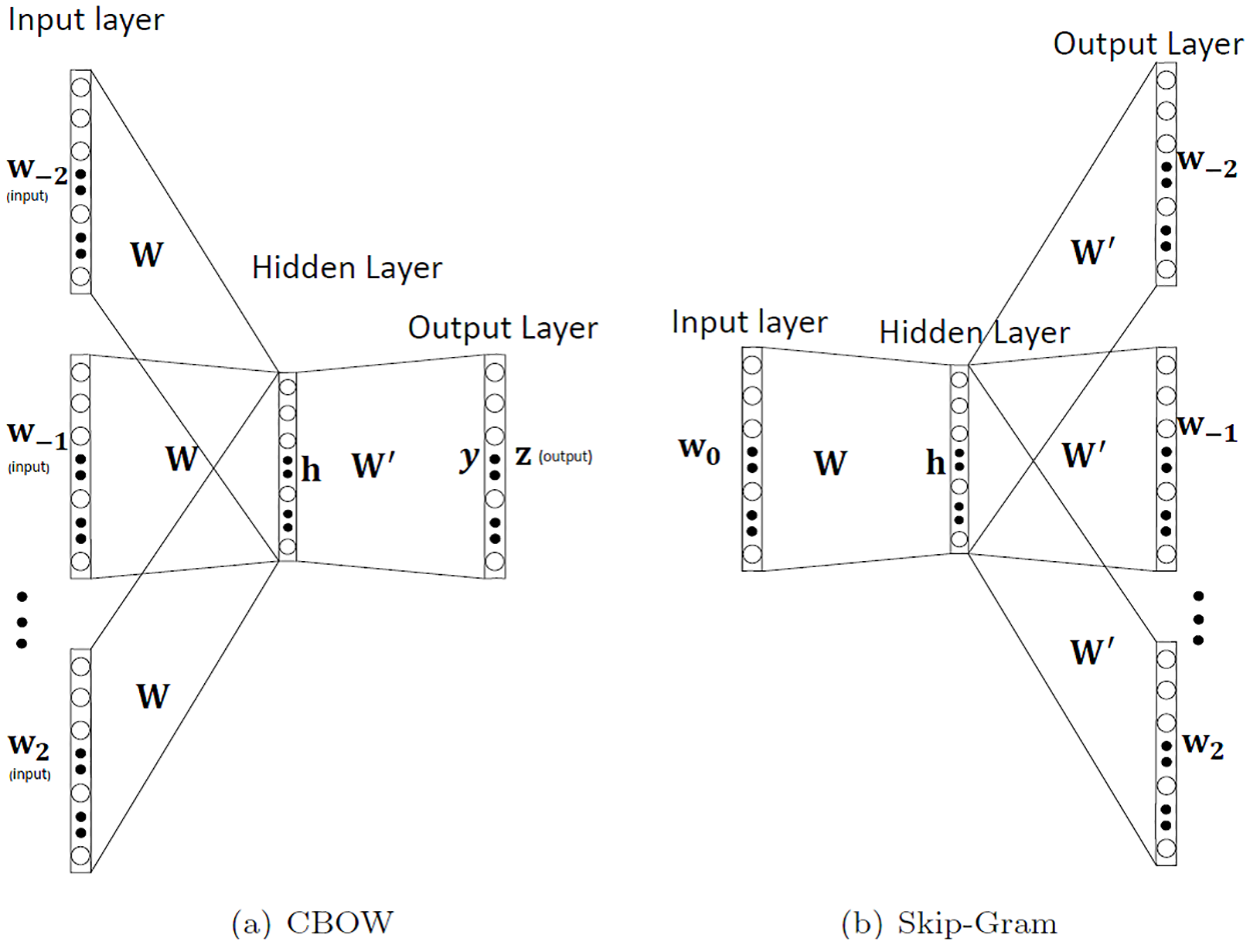
\includegraphics[width=0.92\linewidth]{assets/images/zpracovani-textovych-dat/word2vec-cbow-skipgram.png}
  \caption[CBOW a Skip-gram ve Word2Vec]{Dvě varianty architektury Word2Vec. Popis obrázku: CBOW na levé
  straně používá okolní slova k predikci prostředního slova, zatímco Skip-gram na pravé straně používá
  prostřední slovo k predikci jeho okolního kontextu. Zdroj obrázku: Kimothi, Biyani, Hogan, Soni, Kelly,
  \href{https://doi.org/10.1371/journal.pone.0216636.g001}{PLOS ONE / Figshare}, licence CC BY 4.0.}
  \label{fig:q18-word2vec}
\end{figure}

\subsubsection{CBOW}

CBOW:
\[
(w_{t-r},\ldots,w_{t-1},w_{t+1},\ldots,w_{t+r})
\rightarrow
w_t.
\]

Model dostane okolní slova a snaží se odhadnout slovo uprostřed.

Vlastnosti:
\begin{itemize}
    \item rychlejší trénování,
    \item dobré pro častá slova.
\end{itemize}

\subsubsection{Skip-gram}

Skip-gram:
\[
w_t
\rightarrow
(w_{t-r},\ldots,w_{t-1},w_{t+1},\ldots,w_{t+r}).
\]

Model dostane slovo a snaží se odhadnout jeho kontext.

Vlastnosti:
\begin{itemize}
    \item lepší pro méně častá slova,
    \item potřebuje méně dat pro zachycení vzácnějších vztahů,
    \item často používá negative sampling pro zrychlení trénování.
\end{itemize}

\subsection{GloVe}

GloVe je metoda založená na matici spoluvýskytů slov. Využívá globální informaci o tom, která slova se
vyskytují ve stejných kontextech.

Obecná idea:
\[
X_{ij}
=
\operatorname{cooc}(i,j).
\]

GloVe hledá vektory, které dobře vysvětlují poměry spoluvýskytů.

\subsection{Omezení klasických embeddingů}

Word2Vec a GloVe jsou typicky \textbf{context-free}. Každé slovo má jeden vektor bez ohledu na význam.

Problém:
\[
\text{bank}
\]
může znamenat:
\begin{itemize}
    \item finanční instituci,
    \item břeh řeky.
\end{itemize}

Context-free embedding má pro oba významy jeden vektor.

\subsection{Kontextové embeddingy a transformery}

Moderní modely jako BERT nebo GPT vytvářejí kontextové reprezentace. Stejné slovo může mít různý vektor
podle věty.

\[
\text{bank}_{\text{finance}}
\neq
\text{bank}_{\text{river}}.
\]

Transformer používá mechanismus attention:
\[
Attention(Q,K,V)
=
softmax
\left(
\frac{QK^\top}{\sqrt{d_k}}
\right)V.
\]

\paragraph{Intuice.}
Každý token se \uv{dívá} na jiné tokeny ve větě a určuje, které jsou pro jeho interpretaci důležité.

\begin{figure}[htbp]
  \centering
  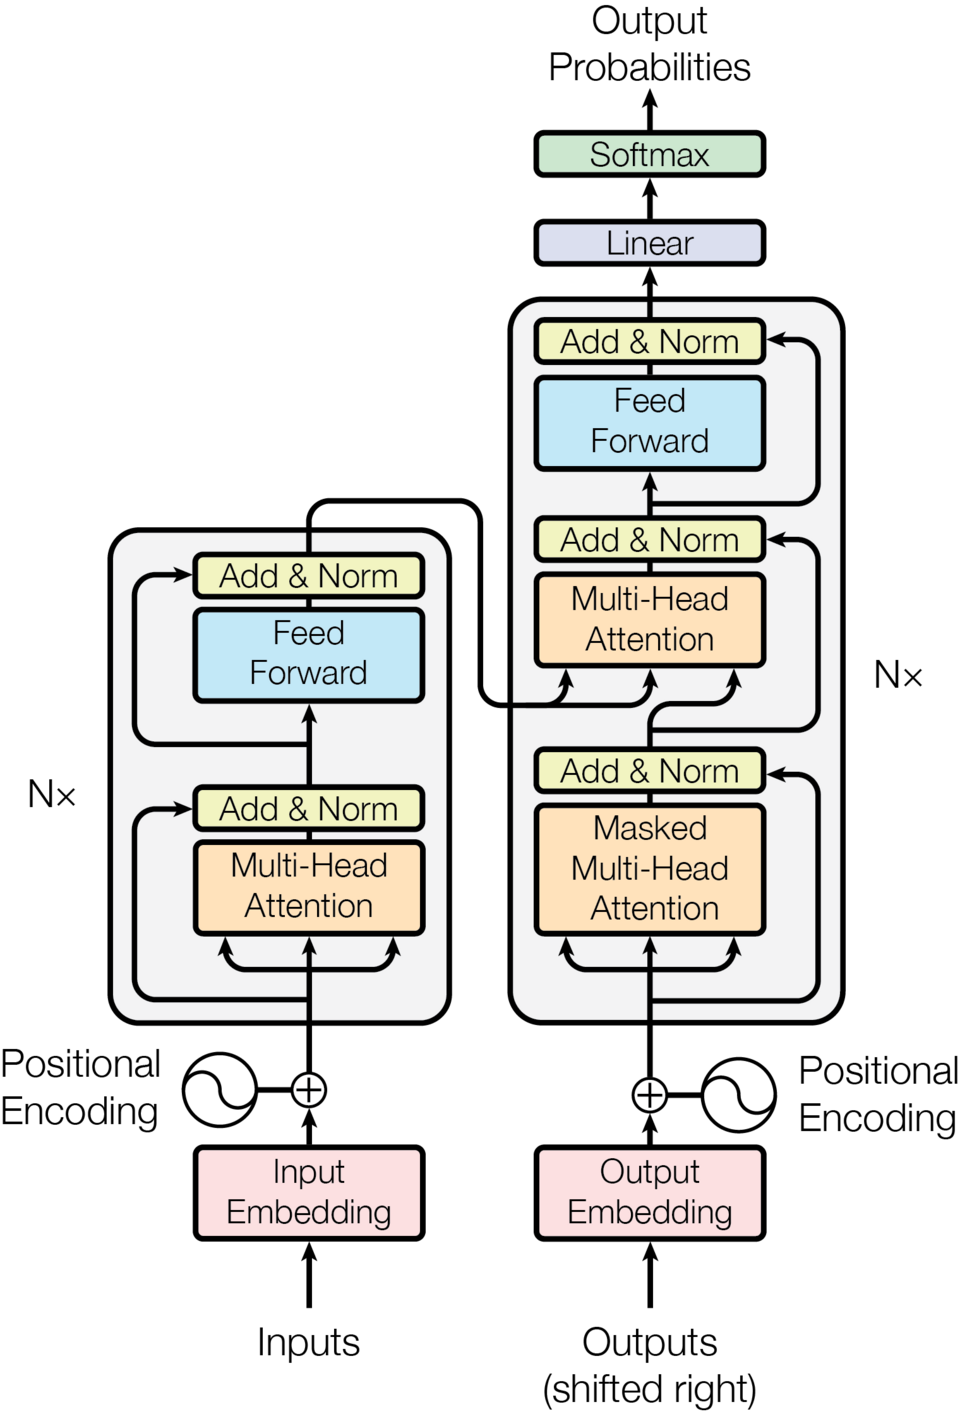
\includegraphics[width=0.54\linewidth]{assets/images/zpracovani-textovych-dat/transformer-architecture.png}
  \caption[Architektura transformeru]{Architektura encoder-decoder transformeru. Popis obrázku: vstupní a
  výstupní tokeny se převádějí na embeddingy s pozičním kódováním, procházejí bloky multi-head attention,
  feed-forward vrstvami a normalizacemi; decoder navíc používá maskovanou attention pro autoregresivní
  generování. Zdroj obrázku: Google,
  \href{https://commons.wikimedia.org/wiki/File:Attention\_Is\_All\_You\_Need\_-\_Encoder-decoder\_Architecture.png}{Wikimedia
  Commons}, licence CC BY-SA 4.0.}
  \label{fig:q18-transformer}
\end{figure}

\subsection{Typy jazykových modelů}

\begin{itemize}
    \item \textbf{N-gramové modely} -- pravděpodobnost dalšího slova podle krátké historie.
    
    \item \textbf{Word2Vec / GloVe} -- učí vektorové reprezentace slov.
    
    \item \textbf{Encoder-only transformery} -- například BERT; vhodné pro klasifikaci, NER a porozumění textu.
    
    \item \textbf{Decoder-only transformery} -- například GPT; vhodné pro generování textu.
    
    \item \textbf{Encoder-decoder transformery} -- vhodné pro překlad, sumarizaci a převod jedné sekvence na jinou.
    
    \item \textbf{Sentence embeddings} -- například Sentence-BERT; vhodné pro podobnost vět, sémantické vyhledávání
    a clustering dokumentů.
\end{itemize}

\subsection{Analytické metody nad textem}

\subsubsection{Textová klasifikace}

Textová klasifikace přiřazuje dokumentu třídu:
\[
d_i \rightarrow y_i.
\]

Příklady:
\begin{itemize}
    \item spam / ne-spam,
    \item téma článku,
    \item typ zákaznického požadavku,
    \item pozitivní / negativní sentiment,
    \item rizikový / nerizikový dokument.
\end{itemize}

Modely:
\begin{itemize}
    \item Naive Bayes,
    \item logistická regrese,
    \item SVM,
    \item rozhodovací stromy,
    \item random forest,
    \item gradient boosting,
    \item neuronové sítě,
    \item transformery.
\end{itemize}

Vyhodnocení:
\[
Accuracy,\quad Precision,\quad Recall,\quad F_1.
\]

\subsubsection{Clustering dokumentů}

Clustering hledá skupiny podobných dokumentů bez předem známých tříd.

Postup:
\begin{enumerate}
    \item reprezentovat dokumenty jako TF-IDF nebo embeddingy,
    \item spočítat podobnosti,
    \item použít shlukovací algoritmus,
    \item interpretovat shluky podle nejtypičtějších slov nebo dokumentů.
\end{enumerate}

Použitelné algoritmy:
\begin{itemize}
    \item k-means,
    \item hierarchické shlukování,
    \item DBSCAN,
    \item HDBSCAN.
\end{itemize}

\subsubsection{Topic modeling}

Topic modeling hledá skrytá témata v kolekci dokumentů.

Základní idea:
\[
\text{document}
=
\text{mixture of topics},
\]
\[
\text{topic}
=
\text{distribution over words}.
\]

LDA modeluje:
\[
P(w|d)
=
\sum_{k=1}^{K}
P(w|z=k)P(z=k|d).
\]

Kde:
\begin{itemize}
    \item $z$ je latentní téma,
    \item $P(w|z)$ říká, která slova jsou typická pro téma,
    \item $P(z|d)$ říká, jaká témata jsou zastoupena v dokumentu.
\end{itemize}

\begin{figure}[htbp]
  \centering
  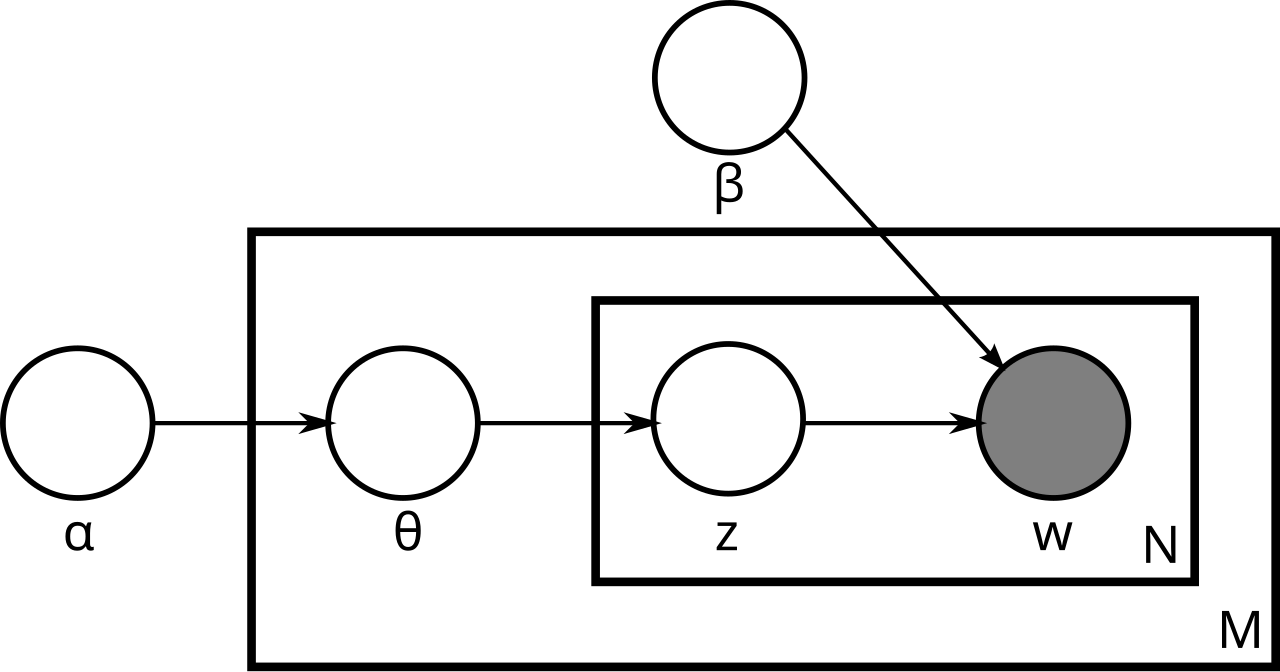
\includegraphics[width=0.78\linewidth]{assets/images/zpracovani-textovych-dat/lda-plate-notation.png}
  \caption[LDA v plate notation]{Grafický model Latent Dirichlet Allocation v plate notation. Popis obrázku:
  dokument má rozdělení témat $\theta$, každé slovo má latentní téma $z$ a pozorované slovo $w$; opakování
  přes slova a dokumenty je vyznačeno obdélníky. Zdroj obrázku: Bkkbrad,
  \href{https://commons.wikimedia.org/wiki/File:Latent\_Dirichlet\_allocation.svg}{Wikimedia Commons},
  licence CC BY-SA 4.0.}
  \label{fig:q18-lda}
\end{figure}

Použití:
\begin{itemize}
    \item explorace velké kolekce textů,
    \item monitoring médií,
    \item analýza zákaznické zpětné vazby,
    \item tematická segmentace dokumentů.
\end{itemize}

\subsubsection{Named Entity Recognition}

NER hledá pojmenované entity:
\[
\text{Oliver Blume} \rightarrow PERSON,
\]
\[
\text{Volkswagen} \rightarrow ORGANIZATION,
\]
\[
\text{23 MEUR} \rightarrow MONEY.
\]

Přístupy:
\begin{itemize}
    \item regulární výrazy,
    \item gazetteery,
    \item pravidla,
    \item CRF,
    \item transformerové modely,
    \item LLM.
\end{itemize}

Vyhodnocení NER:
\[
Precision=
\frac{TP}{TP+FP},
\qquad
Recall=
\frac{TP}{TP+FN},
\qquad
F_1=
2\frac{PR}{P+R}.
\]

Rozlišuje se:
\begin{itemize}
    \item \textbf{strict match} -- přesně stejný rozsah entity i typ,
    \item \textbf{relaxed match} -- částečná shoda rozsahu nebo tolerantnější hodnocení.
\end{itemize}

\subsubsection{Relation extraction}

Relation extraction hledá vztahy mezi entitami:
\[
relation(e_1,e_2).
\]

Příklad:
\[
CEO\_of(\text{Oliver Blume},\text{Volkswagen}).
\]

Přístupy:
\begin{itemize}
    \item pravidlové vzory,
    \item dependency parsing,
    \item supervised learning,
    \item distant supervision,
    \item transformerové modely,
    \item LLM s následnou validací.
\end{itemize}

\subsection{Sentiment analysis}

Sentiment analysis neboli opinion mining se zabývá zjišťováním názorů, postojů, hodnocení a sentimentu
vyjádřeného v textu.

Typické třídy:
\[
positive,\quad negative,\quad neutral.
\]

Sentiment lze analyzovat na různých úrovních:
\begin{itemize}
    \item \textbf{document-level} -- sentiment celého dokumentu;
    \item \textbf{sentence-level} -- sentiment věty;
    \item \textbf{aspect-based} -- sentiment ke konkrétnímu aspektu entity.
\end{itemize}

\subsubsection{Opinion quintuple}

Formální reprezentace názoru:
\[
(e_j,a_{jk},so_{ijkl},h_i,t_l).
\]

Kde:
\begin{itemize}
    \item $e_j$ je cílová entita,
    \item $a_{jk}$ je aspekt entity,
    \item $so_{ijkl}$ je sentimentová hodnota,
    \item $h_i$ je držitel názoru,
    \item $t_l$ je čas vyjádření názoru.
\end{itemize}

Příklad:
\[
(\text{iPhone},\ \text{battery life},\ -,\ \text{user123},\ \text{2025-01-10}).
\]

\subsubsection{Sentimentové lexikony}

Lexikonový přístup používá seznamy slov s polaritou:
\[
\text{good} \rightarrow +,
\qquad
\text{bad} \rightarrow -.
\]

Problémy:
\begin{itemize}
    \item význam závisí na doméně,
    \item slova mohou být ironická,
    \item sentiment může být vyjádřen faktem,
    \item nutné řešit negaci a modifikátory.
\end{itemize}

\subsubsection{Shifters a modifikátory polarity}

Negace:
\[
\text{good}
\rightarrow +,
\qquad
\text{not good}
\rightarrow -.
\]

Zesilovače:
\[
\text{very good}
\]
znamená silnější pozitivní sentiment.

Zeslabovače:
\[
\text{slightly bad}
\]
znamená slabší negativní sentiment.

Adverzativní spojky:
\[
\text{A, but B}
\]
často zvyšují význam části za \uv{but}.

\paragraph{Problém ironie.}
Věta:
\begin{quote}
\uv{Skvělé, aplikace zase spadla.}
\end{quote}
obsahuje pozitivní slovo \uv{skvělé}, ale celkový sentiment je negativní.

\subsection{Sumarizace textu}

Sumarizace převádí dlouhý text nebo kolekci textů na kratší přehled.

Typy:
\begin{itemize}
    \item \textbf{extraktivní sumarizace} -- vybírá důležité věty z původního textu;
    \item \textbf{abstraktivní sumarizace} -- generuje nové formulace.
\end{itemize}

Použití:
\begin{itemize}
    \item shrnutí dokumentů,
    \item shrnutí recenzí,
    \item shrnutí reportů,
    \item monitoring médií.
\end{itemize}

U názorů je často důležitá \textbf{aspect-based sumarizace}, například:
\begin{center}
60 \% uživatelů chválí fotoaparát, 40 \% kritizuje baterii.
\end{center}

\subsection{Question answering a RAG}

Předtrénované jazykové modely mají omezení:
\begin{itemize}
    \item nemusí obsahovat nejnovější informace,
    \item mohou halucinovat,
    \item slabě pokrývají úzké domény,
    \item neumí vždy spolehlivě uvést zdroje,
    \item výstup může být příliš obecný.
\end{itemize}

Retrieval-Augmented Generation, RAG, kombinuje jazykový model s vyhledáváním.

Postup:
\[
\begin{aligned}
\text{query}
&\rightarrow
\text{retrieval}
\rightarrow
\text{relevant passages},\\
\text{query + passages}
&\rightarrow
\text{prompt augmentation}
\rightarrow
\text{generation}.
\end{aligned}
\]

\begin{figure}[htbp]
  \centering
  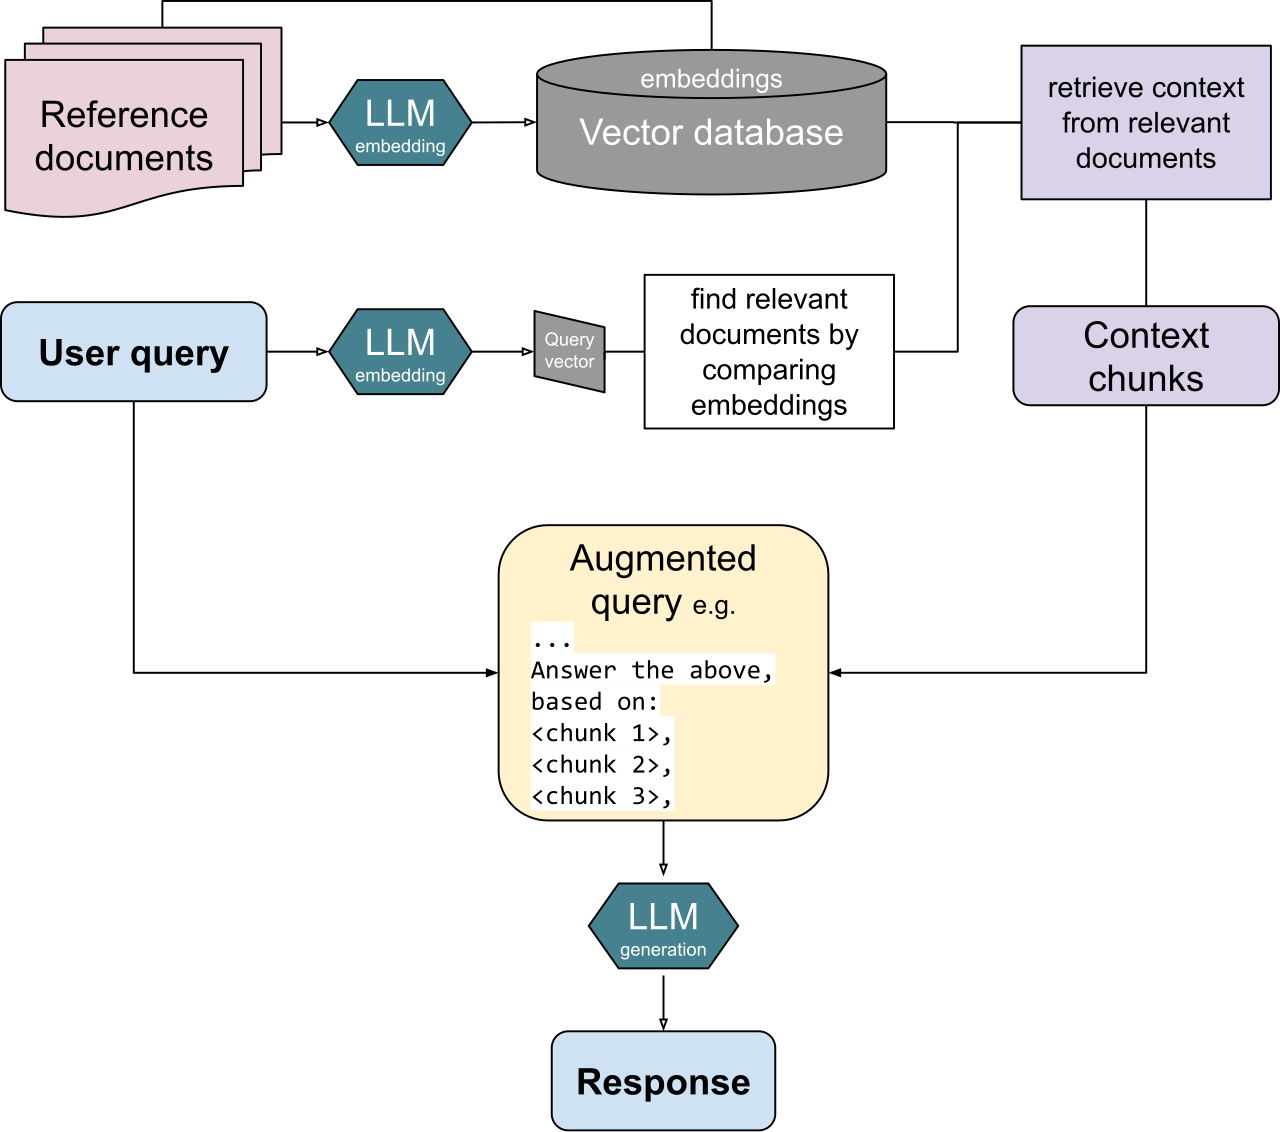
\includegraphics[width=0.82\linewidth]{assets/images/zpracovani-textovych-dat/rag-diagram.png}
  \caption[Retrieval-Augmented Generation]{Zjednodušené schéma RAG. Popis obrázku: referenční dokumenty se
  převedou na embeddingy a uloží do vektorové databáze; dotaz uživatele se také převede na vektor, podle
  podobnosti se vyhledají relevantní části dokumentů a ty se spolu s dotazem vloží do promptu pro jazykový
  model. Zdroj obrázku: Turtlecrown,
  \href{https://commons.wikimedia.org/wiki/File:RAG\_diagram.svg}{Wikimedia Commons}, licence CC BY-SA 4.0.}
  \label{fig:q18-rag}
\end{figure}

RAG umožňuje využít:
\begin{itemize}
    \item novější texty,
    \item doménově specifické dokumenty,
    \item kurátorsky ověřené zdroje,
    \item lokální firemní dokumentaci.
\end{itemize}

\subsubsection{Sparse a dense retrieval v RAG}

Sparse retrieval:
\[
TF\text{-}IDF,\quad BM25.
\]

Dense retrieval:
\[
\text{Sentence-BERT embeddings},\quad \text{vector database}.
\]

Dense retrieval je vhodný pro sémantickou podobnost, sparse retrieval je často lepší pro přesná klíčová
slova, kódy a názvy.

\subsection{Knowledge graphs a KG-RAG}

Znalostní graf ukládá fakta jako uzly a hrany:
\[
(entity_1) \xrightarrow{relation} (entity_2).
\]

Příklad:
\[
(\text{Volkswagen}) \xrightarrow{CEO} (\text{Oliver Blume}).
\]

KG-RAG využívá místo nebo vedle textového korpusu strukturovaný znalostní graf. Výhody:
\begin{itemize}
    \item přesnější a kurátorovanější fakta,
    \item lepší vysvětlitelnost,
    \item možnost grafového dotazování,
    \item menší riziko halucinací než u volného textu.
\end{itemize}

\subsection{Vyhodnocení textových metod}

\subsubsection{Klasifikace}

\[
Accuracy=
\frac{TP+TN}{TP+TN+FP+FN}.
\]

\[
Precision=
\frac{TP}{TP+FP}.
\]

\[
Recall=
\frac{TP}{TP+FN}.
\]

\[
F_1=
2\frac{Precision\cdot Recall}{Precision+Recall}.
\]

\subsubsection{IR}

U vyhledávání:
\begin{itemize}
    \item precision@k,
    \item recall@k,
    \item MAP,
    \item NDCG,
    \item MRR.
\end{itemize}

Precision@k:
\[
Precision@k
=
\frac{\#\text{ relevant documents in top } k}
{k}.
\]

\subsubsection{NER a IE}

U NER:
\begin{itemize}
    \item strict span match,
    \item relaxed span match,
    \item micro/macro precision, recall, F1.
\end{itemize}

U relation extraction:
\begin{itemize}
    \item správnost dvojice entit,
    \item správnost typu vztahu,
    \item správnost celého trojčlenu.
\end{itemize}

\subsubsection{Sumarizace a generování}

Používají se automatické metriky:
\begin{itemize}
    \item ROUGE,
    \item BLEU,
    \item BERTScore.
\end{itemize}

U generativních modelů je však často nutné lidské hodnocení:
\begin{itemize}
    \item věcná správnost,
    \item úplnost,
    \item čitelnost,
    \item relevance,
    \item citace zdrojů,
    \item bezpečnost.
\end{itemize}

\subsection{Existující nástroje}

\subsubsection{Python}

\begin{itemize}
    \item \texttt{re} -- regulární výrazy;
    \item \texttt{pandas} -- práce s tabulkovými výstupy;
    \item \texttt{scikit-learn} -- TF-IDF, klasifikace, clustering;
    \item \texttt{NLTK} -- základní NLP a výuka;
    \item \texttt{spaCy} -- tokenizace, POS tagging, NER, dependency parsing;
    \item \texttt{Stanza} -- NLP pipeline od Stanford NLP;
    \item \texttt{UDPipe} -- tokenizace, lemmatizace, POS tagging a parsing, vhodné i pro češtinu;
    \item \texttt{Gensim} -- Word2Vec, topic modeling;
    \item \texttt{transformers} -- modely BERT, GPT a další;
    \item \texttt{sentence-transformers} -- sentence embeddings;
    \item \texttt{Haystack}, \texttt{LangChain}, \texttt{LlamaIndex} -- RAG aplikace.
\end{itemize}

\subsubsection{R}

\begin{itemize}
    \item \texttt{tidytext},
    \item \texttt{quanteda},
    \item \texttt{tm},
    \item \texttt{text2vec},
    \item \texttt{udpipe},
    \item \texttt{stm}.
\end{itemize}

\subsubsection{Vyhledávání a indexace}

\begin{itemize}
    \item Apache Lucene,
    \item Elasticsearch,
    \item OpenSearch,
    \item Solr,
    \item FAISS,
    \item Milvus,
    \item Pinecone,
    \item Weaviate,
    \item Chroma.
\end{itemize}

Lucene/Elasticsearch jsou typické pro sparse retrieval a fulltextové vyhledávání. FAISS a vektorové
databáze jsou typické pro dense retrieval nad embeddingy.

\subsubsection{Anotace dat}

\begin{itemize}
    \item doccano,
    \item Label Studio,
    \item Prodigy,
    \item brat,
    \item INCEpTION,
    \item GATE.
\end{itemize}

Anotace je důležitá pro supervised úlohy jako sentiment, NER, relation extraction nebo klasifikace dokumentů.

\subsection{Typické problémy při zpracování textu}

\begin{itemize}
    \item mnoho jazykových variant,
    \item překlepy a neformální jazyk,
    \item ironie a sarkasmus,
    \item doménová specifika,
    \item nejednoznačnost slov,
    \item coreference,
    \item nedostatek anotovaných dat,
    \item nevyvážené třídy,
    \item změna témat v čase,
    \item bias v datech,
    \item ochrana osobních údajů.
\end{itemize}

\subsection{Tradiční NLP vs. deep learning}

\subsubsection{Tradiční přístup}

Tradiční NLP často používá:
\begin{itemize}
    \item ruční nebo lingvistické příznaky,
    \item tokenizaci,
    \item lemmatizaci,
    \item POS tagging,
    \item syntaktické příznaky,
    \item TF-IDF,
    \item klasické ML modely.
\end{itemize}

Výhody:
\begin{itemize}
    \item lepší interpretovatelnost,
    \item nižší výpočetní náklady,
    \item použitelné na menších datech.
\end{itemize}

Nevýhody:
\begin{itemize}
    \item vyžaduje feature engineering,
    \item hůře zachycuje hlubší význam,
    \item často horší výkon u složitých úloh.
\end{itemize}

\subsubsection{Deep learning přístup}

Moderní modely, hlavně transformery, pracují více end-to-end:
\[
\text{text}
\rightarrow
\text{tokenizer}
\rightarrow
\text{transformer}
\rightarrow
\text{output}.
\]

Výhody:
\begin{itemize}
    \item vysoký výkon,
    \item kontextové reprezentace,
    \item transfer learning,
    \item méně ručního feature engineeringu.
\end{itemize}

Nevýhody:
\begin{itemize}
    \item vyšší nároky na výpočetní výkon,
    \item horší interpretovatelnost,
    \item riziko halucinací u generativních modelů,
    \item potřeba kontroly biasu a bezpečnosti.
\end{itemize}

\subsection{Doporučený praktický postup}

\begin{enumerate}
    \item definovat úlohu: klasifikace, vyhledávání, extrakce, sumarizace;
    \item zkontrolovat zdroj a kvalitu dat;
    \item vyčistit a normalizovat text;
    \item vytvořit vhodnou reprezentaci textu;
    \item zvolit baseline model, například TF-IDF + logistická regrese;
    \item porovnat s pokročilejší metodou, například embeddingy nebo transformer;
    \item vyhodnotit na oddělených datech;
    \item analyzovat chyby;
    \item ošetřit právní, etické a bezpečnostní aspekty;
    \item připravit nasazení a monitoring.
\end{enumerate}

\subsection{Shrnutí ke zkoušce}

Zpracování textových dat převádí přirozený jazyk do podoby vhodné pro vyhledávání, modelování a extrakci
informací. Základní NLP pipeline zahrnuje tokenizaci, rozdělení vět, normalizaci, lemmatizaci, POS tagging,
syntaktické zpracování, NER, relation extraction a coreference resolution.

Text lze reprezentovat klasicky pomocí bag-of-words, n-gramů a TF-IDF:
\[
w_{ij}=tf_{ij}\cdot idf_j,
\]
nebo moderně pomocí embeddingů:
\[
w \mapsto \mathbf{e}_w\in\mathbb{R}^k.
\]

Word2Vec využívá CBOW nebo Skip-gram a učí slovní vektory z kontextu. Moderní transformery vytvářejí
kontextové reprezentace a jsou základem současných jazykových modelů. RAG kombinuje vyhledávání dokumentů
s generováním odpovědi:
\[
Retrieval \rightarrow Augmentation \rightarrow Generation.
\]

Mezi hlavní analytické metody patří klasifikace textu, sentiment analysis, topic modeling, clustering,
NER, relation extraction, sumarizace, question answering a sémantické vyhledávání. Prakticky se používají
nástroje jako Python knihovny scikit-learn, spaCy, Gensim, transformers a sentence-transformers,
vyhledávací systémy Elasticsearch a FAISS, R balíčky tidytext a quanteda nebo anotovací nástroje doccano
a Label Studio.

\subsection{Zdroje}

\begin{itemize}
    \item Jurafsky, Martin:
    \href{https://web.stanford.edu/~jurafsky/slp3/ed3book.pdf}{Speech and Language Processing}.
    \item spaCy dokumentace:
    \href{https://spacy.io/usage/linguistic-features}{Linguistic Features}.
    \item scikit-learn dokumentace:
    \href{https://scikit-learn.org/stable/modules/feature\_extraction.html\#text-feature-extraction}{Text
    feature extraction}.
    \item Gensim dokumentace:
    \href{https://radimrehurek.com/gensim/models/word2vec.html}{Word2Vec}.
    \item Vaswani et al.:
    \href{https://arxiv.org/abs/1706.03762}{Attention Is All You Need}.
    \item Lewis et al.:
    \href{https://arxiv.org/abs/2005.11401}{Retrieval-Augmented Generation for Knowledge-Intensive NLP Tasks}.
    \item Blei, Ng, Jordan:
    \href{https://www.jmlr.org/papers/v3/blei03a.html}{Latent Dirichlet Allocation}.
    \item Bing Liu:
    \href{https://www.cs.uic.edu/~liub/FBS/SentimentAnalysis-and-OpinionMining.pdf}{Sentiment Analysis and
    Opinion Mining}.
    \item Wikimedia Commons:
    \href{https://commons.wikimedia.org/wiki/File:Basic\_constituent\_structure\_analysis\_English\_sentence.svg}{Basic
    constituent structure analysis English sentence}.
    \item PLOS ONE / Figshare:
    \href{https://doi.org/10.1371/journal.pone.0216636.g001}{Word2Vec architecture}.
    \item Wikimedia Commons:
    \href{https://commons.wikimedia.org/wiki/File:Attention\_Is\_All\_You\_Need\_-\_Encoder-decoder\_Architecture.png}{Attention
    Is All You Need -- Encoder-decoder Architecture}.
    \item Wikimedia Commons:
    \href{https://commons.wikimedia.org/wiki/File:Latent\_Dirichlet\_allocation.svg}{Latent Dirichlet allocation}.
    \item Wikimedia Commons:
    \href{https://commons.wikimedia.org/wiki/File:RAG\_diagram.svg}{RAG diagram}.
\end{itemize}

\newpage

\section{Big data. Charakteristika velkých dat, metody a nástroje pro jejich zpracování}

\subsection*{Charakteristika velkých dat}
Dodaný materiál téma big data pokrývá nepřímo přes datové zdroje, transakční databáze, NoSQL, BI, data mining a kvalitu dat. Z těchto částí lze postavit základní odpověď: big data jsou data, jejichž objem, rychlost vzniku, různorodost nebo složitost překračují možnosti běžného zpracování v tradičních relačních databázích.

Velká data se obvykle popisují pomocí vlastností:
\begin{itemize}
  \item \term{Volume} - velký objem dat;
  \item \term{Velocity} - vysoká rychlost vzniku, přenosu nebo požadované reakce;
  \item \term{Variety} - různorodost datových typů, například tabulky, JSON, logy, texty, obrázky nebo streamy;
  \item \term{Veracity} - nejistota, kvalita a důvěryhodnost dat;
  \item \term{Value} - schopnost získat z dat použitelnou hodnotu pro rozhodování.
\end{itemize}

\subsection*{Vztah k dodaným materiálům}
Materiály rozlišují interní a externí datové zdroje, strukturovaná, semistrukturovaná a nestrukturovaná data. To je pro big data důležité: velká data typicky nevznikají jen v jedné relační tabulce, ale kombinují transakce, logy, texty, JSON/XML dokumenty, webová data a případně senzorová data.

\subsection*{NoSQL a specializované databáze}
V materiálech se objevují NoSQL databáze a specializované databáze. NoSQL databáze často nepoužívají klasické tabulkové struktury, normalizaci a SQL v tradičním smyslu. Místo toho mohou ukládat dokumenty, klíč-hodnota páry, grafy nebo jiné specializované struktury. Výhodou bývá flexibilnější schéma a škálovatelnost, nevýhodou slabší návaznost na relační model a často jiný způsob zajištění konzistence.

\begin{itemize}
  \item dokumentové databáze - ukládají komplexní dokumenty, často JSON/BSON;
  \item key-value databáze - rychlé ukládání hodnot podle klíče, často pro cache;
  \item grafové databáze - pracují s uzly a hranami, hodí se pro vztahy a sítě;
  \item specializované databáze - řeší konkrétní typ dat nebo přístupu.
\end{itemize}

\subsection*{Big data v analytice}
Big data se v datové analytice využívají pro reporting ve velkém měřítku, strojové učení, doporučovací systémy, detekci anomálií, personalizaci, monitoring provozu a analýzu textu nebo webových dat. Základní problém je převést velký a různorodý datový zdroj na použitelnou datovou sadu se známou kvalitou, významem proměnných a reprodukovatelným zpracováním.

\todohead
\begin{itemize}
  \item Doplnit Hadoop, HDFS, MapReduce, Spark a distribuované výpočty.
  \item Doplnit data lake, lakehouse a cloudová datová úložiště.
  \item Doplnit streamingové zpracování: Kafka, Spark Streaming, Flink.
  \item Doplnit CAP teorém, eventual consistency a rozdíl oproti ACID.
\end{itemize}

\newpage

\section{Business intelligence. Principy, technologické komponenty, nástroje}

\subsection*{Smysl BI v podniku}
Materiály vysvětlují BI jako technologii a přístup, který integruje data z podnikových oblastí a poskytuje managementu informace v požadované struktuře. Podniky uchovávají velké množství dat v systémech ERP, CRM, SCM a dalších aplikacích. Tato data jsou typicky v transakčních databázích OLTP, které jsou vhodné pro provozní změny, ale nevhodné pro složité souhrnné analýzy.

BI řeší dva hlavní problémy:
\begin{itemize}
  \item analytická data pocházejí z různých systémů s odlišnou strukturou;
  \item management potřebuje rychlé, přesné a srozumitelné informace pro rozhodování.
\end{itemize}

Bez BI mohou být informace nedostupné, získávané pomalu nebo nekonzistentní, což vede k intuitivnímu rozhodování nepodloženému fakty. BI má umožnit rozhodování založené na datech.

\subsection*{Princip BI: multidimenzionální pohled}
Základním principem BI je multidimenzionální pohled na data. To znamená, že sledované ukazatele lze zobrazovat podle různých dimenzí. Například tržby lze analyzovat podle času, regionu, produktu, zákazníka, prodejního kanálu nebo organizační jednotky.

Technologie založená na multidimenzionálních databázích se nazývá OLAP - \textit{On-Line Analytical Processing}. OLAP umožňuje rychlé analytické dotazy, agregace, drill-down, roll-up a změnu pohledu na stejná data.

\subsection*{Architektura BI}
Materiály popisují tok dat ve zjednodušené podobě:
\[
\text{zdrojové systémy} \rightarrow \text{ETL} \rightarrow \text{datový sklad} \rightarrow \text{OLAP} \rightarrow \text{analýzy a reporting}
\]

\term{Produkční databáze} jsou zdrojové systémy, například ERP, SCM, CRM, finanční systémy nebo externí systémy. Jsou optimalizované pro provozní zpracování a ukládání dat v reálném čase, nikoli pro analytické úlohy.

\term{ETL} je datová pumpa. Jejím úkolem je data získat, transformovat a nahrát do analytických struktur. Pracuje často dávkově v pravidelných intervalech.

\term{DSA} je dočasné úložiště extrahovaných dat. Data zde bývají detailní, aktuální, často nekonzistentní a ve stejné struktuře jako ve zdrojových systémech.

\term{ODS} je operativní úložiště aktuálních a konsolidovaných dat. Může sloužit pro jednoduché dotazy nad aktuálními daty nebo jako centrální databáze referenčních údajů.

\term{Datový sklad} je integrovaný, subjektově orientovaný, stálý a časově rozlišený souhrn dat pro podporu managementu.

\term{Datové tržiště} je menší datový sklad určený pro omezený okruh uživatelů nebo specifickou oblast.

\term{OLAP databáze} obsahuje jednu nebo více OLAP kostek. Kostky často obsahují předzpracované agregace podle hierarchií dimenzí.

\subsection*{Reporting a analýzy}
Reporting je dotazování do databází a prezentace výsledků. Materiály rozlišují:
\begin{itemize}
  \item \term{standardní reporting} - předdefinované reporty v pravidelných intervalech;
  \item \term{ad hoc reporting} - jednorázový specifický dotaz vytvořený uživatelem.
\end{itemize}

BI dále souvisí s data miningem. Datový sklad poskytuje kvalitní zdroj pro analytické metody, které hledají strategické informace a skryté vztahy v datech.

\subsection*{Vazba BI na podnikové aplikace}
Materiály uvádějí BI jako jednu z rozšiřujících oblastí ERP II vedle CRM a SCM. ERP poskytuje provozní data z financí, nákupu, výroby, logistiky a HR. CRM poskytuje zákaznická data. SCM poskytuje data o dodavatelském řetězci. BI tato data integruje a převádí do podoby vhodné pro rozhodování.

\todohead
\begin{itemize}
  \item Doplnit hvězdicové a sněhové schéma, fact table a dimension table.
  \item Doplnit OLAP operace: slice, dice, drill-down, roll-up, pivot.
  \item Doplnit moderní BI nástroje: Power BI, Tableau, Qlik, Looker.
  \item Doplnit rozdíl DWH, data lake a lakehouse.
  \item Doplnit governance v BI: metadata, datový katalog, kvalita dat, vlastnictví dat.
\end{itemize}

\newpage

\section{Řízení datového projektu. Životní cyklus, metodiky a standardy, organizace projektu a nástroje pro podporu řízení}

\subsection*{Datový projekt jako projekt dobývání znalostí}
Dodaný materiál nemá samostatnou kapitolu „řízení datového projektu“, ale obsahuje CRISP-DM, metodiky budování IS, životní cyklus aplikace, agilní metodiky, Scrum a části o organizaci analytické práce. Pro datovou analytiku je nejlépe použitelný CRISP-DM.

Datový projekt typicky nezačíná modelem, ale problémem zadavatele. Cílem je převést business otázku na analytickou úlohu, získat a připravit data, vytvořit výstup nebo model, vyhodnotit ho a zajistit využití v praxi.

\subsection*{Životní cyklus podle CRISP-DM}
CRISP-DM lze použít jako hlavní kostru řízení datového projektu:

\begin{enumerate}
  \item \term{Porozumění businessu} - domluvit cíl, očekávání, kritéria úspěchu, omezení, cenu analýzy a rizika. V materiálech je zdůrazněna komunikace s vlastníkem dat a doménovým expertem.
  \item \term{Porozumění datům} - zjistit dostupná data, jejich strukturu, rozsah, formát, význam polí, granularitu a kvalitu.
  \item \term{Příprava dat} - čistit data, řešit chybějící hodnoty, duplicity, chybná data, transformovat formáty, diskretizovat, vytvářet odvozené proměnné a doplňovat externí data.
  \item \term{Modelování} - vybrat analytické metody odpovídající cíli a povaze dat. Modelování je jen jedna část projektu, ne celý projekt.
  \item \term{Vyhodnocení} - posoudit, zda výsledky odpovídají business cíli, zda jsou srozumitelné a důvěryhodné.
  \item \term{Nasazení / využití} - předat výstupy, zapracovat do rozhodování, reportingu, procesu nebo aplikace.
\end{enumerate}

Materiály uvádějí, že příprava dat a komunikace se zadavatelem jsou velmi pracné části. Samotné modelování může tvořit menší část práce než čištění, pochopení problému a interpretace.

\subsection*{Organizace projektu a role}
Z materiálů k MMDIS a projektům lze odvodit role použitelné i pro datový projekt:
\begin{itemize}
  \item \term{zadavatel / sponzor} - určuje smysl projektu, rozhoduje o zdrojích a očekávaném přínosu;
  \item \term{vlastník business procesu} - zná proces, ve kterém mají být výsledky použity;
  \item \term{vlastník dat} - odpovídá za dostupnost a význam dat;
  \item \term{doménový expert} - pomáhá interpretovat proměnné a výsledky;
  \item \term{datový analytik / data scientist} - provádí analýzu, modelování a interpretaci;
  \item \term{datový inženýr} - připravuje datové pipeline, integraci a úložiště;
  \item \term{uživatel výstupu} - používá report, dashboard, model nebo doporučení.
\end{itemize}

Důležitá je průběžná komunikace. Materiály u CRISP-DM zdůrazňují budování důvěry vlastníka dat a doménového experta, protože bez důvěry se výsledky nemusí použít.

\subsection*{Metodiky řízení: rigorózní a agilní přístup}
Materiály rozlišují rigorózní a agilní metodiky. Pro datový projekt je užitečné znát rozdíl.

\term{Rigorózní metodiky} předpokládají, že procesy lze popsat, plánovat, řídit a měřit. Mají více dokumentace, formalit a předem definovaných kroků. Hodí se pro stabilnější prostředí, větší projekty a situace s nutností silné kontroly.

\term{Agilní metodiky} kladou důraz na fungující výstup, častou komunikaci, reakci na změnu, spolupráci se zákazníkem, krátké iterace a samoorganizující se týmy. V datových projektech se hodí, protože data i požadavky se často během práce zpřesňují.

Scrum lze popsat jako rámec s Product Ownerem, týmem a Scrum Masterem. Práce probíhá ve sprintech, na začátku se plánuje sprint backlog, každý den probíhá krátká porada a na konci sprintu review a retrospektiva.

\subsection*{Standardy a výstupy}
Z dodaných materiálů lze jako standard pro data mining uvést CRISP-DM. Dále materiály uvádějí metodiky IS/ICT a IT governance rámce jako ITIL a COBIT, ale ty jsou pro datový projekt spíše doplňkové.

Typické výstupy datového projektu:
\begin{itemize}
  \item zadání a business cíle;
  \item popis dat a datových zdrojů;
  \item datový slovník;
  \item dokumentace čištění a transformací;
  \item analytický dataset;
  \item model nebo report;
  \item vyhodnocení kvality modelu;
  \item doporučení a plán využití výsledků.
\end{itemize}

\todohead
\begin{itemize}
  \item Doplnit standardy a metodiky mimo CRISP-DM: SEMMA, TDSP, případně DAMA-DMBOK pro data management.
  \item Doplnit nástroje řízení projektu: Jira, Trello, MS Project, Git, GitLab/GitHub, MLflow, DVC, Airflow.
  \item Doplnit MLOps a životní cyklus modelu po nasazení: monitoring, drift, retraining, verzování dat a modelů.
  \item Doplnit rizika datového projektu: nedostupná data, nízká kvalita, nejasný cíl, právní omezení, nepřijetí uživateli.
\end{itemize}

\newpage

\section{Optimalizační modely pro podporu ekonomického rozhodování. Příklady typických úloh LP a MILP, heuristické optimalizační algoritmy}

\subsection{Základní myšlenka optimalizace}

Optimalizace slouží k tomu, abychom z množiny přípustných rozhodnutí vybrali takové, které je
nejlepší vzhledem ke zvolenému kritériu. V ekonomii a managementu jde typicky o maximalizaci
zisku, výnosu nebo užitku, případně minimalizaci nákladů, času, rizika, vzdálenosti či ztráty.

Obecný optimalizační problém lze zapsat jako
\[
\begin{aligned}
\min/\max \quad & f(x)\\
\text{s.t.}\quad & g_i(x)\le 0,\quad i=1,\dots,m,\\
& h_j(x)=0,\quad j=1,\dots,p,\\
& x\in X.
\end{aligned}
\]

Kde:
\begin{itemize}
    \item $x$ je vektor rozhodovacích proměnných,
    \item $f(x)$ je účelová funkce,
    \item $g_i(x)$ a $h_j(x)$ jsou omezení,
    \item $X$ určuje typ proměnných, například spojité, celočíselné nebo binární.
\end{itemize}

Typický postup při tvorbě optimalizačního modelu:
\[
\text{reálný problém}
\rightarrow
\text{rozhodovací proměnné}
\rightarrow
\text{účelová funkce}
\rightarrow
\text{omezení}
\rightarrow
\text{výpočet a interpretace řešení}.
\]

Například firma může rozhodovat, kolik vyrobit jednotlivých produktů. Proměnné jsou vyráběná
množství, účelová funkce je zisk a omezení vyjadřují dostupné zdroje, kapacity strojů nebo maximální
poptávku.

\subsection{Lineární programování}

Lineární programování, zkráceně LP, řeší optimalizační úlohy, ve kterých je účelová funkce i všechna
omezení lineární. Standardní maximalizační tvar je
\[
\begin{aligned}
\max_x \quad & c^\top x\\
\text{s.t.}\quad & Ax\le b,\\
& x\ge 0.
\end{aligned}
\]

Kde:
\begin{itemize}
    \item $c$ je vektor koeficientů účelové funkce, například jednotkových zisků,
    \item $A$ je matice technologických nebo strukturálních koeficientů,
    \item $b$ je vektor pravých stran, například dostupných kapacit,
    \item $x$ je vektor rozhodovacích proměnných.
\end{itemize}

Nerovnosti lze převést na rovnosti pomocí doplňkových proměnných:
\[
Ax+s=b,\qquad s\ge 0.
\]
Proměnná $s_i$ říká, kolik zůstalo nevyužité kapacity v $i$-tém omezení. Pokud je $s_i=0$, dané
omezení je aktivní; pokud je $s_i>0$, zdroj není plně využit.

\subsubsection{Geometrická interpretace LP}

Přípustná množina lineárního programu je průnik polorovin, tedy konvexní mnohostěn. Pro LP platí
důležitá vlastnost:

\[
\text{pokud existuje optimální řešení, existuje také v některém vrcholu přípustné množiny.}
\]

Proto není nutné prohledávat všechny body přípustné množiny. Stačí se zaměřit na vrcholy, které
odpovídají tzv. bazickým přípustným řešením.

Možné koncové stavy LP:
\begin{itemize}
    \item jedno optimální řešení,
    \item více optimálních řešení,
    \item neomezené řešení,
    \item žádné přípustné řešení.
\end{itemize}

\subsection{Bazické řešení a bazické přípustné řešení}

Po převodu omezení do tvaru
\[
A'x=b,\qquad x\ge 0
\]
vybíráme určité proměnné jako bazické. Ostatní, nebazické proměnné, nastavíme na nulu.
Pokud výsledné řešení splňuje nezápornost, jde o \textbf{bazické přípustné řešení}.

Je-li v modelu po zavedení slack proměnných $n$ proměnných a $m$ omezení ve tvaru rovností,
pak bázi tvoří $m$ lineárně nezávislých sloupců matice $A'$. Počet možných bází může být velmi
velký:
\[
\binom{n}{m}.
\]
Proto by prosté vyzkoušení všech bazických řešení bylo pro větší úlohy nepraktické.

\subsection{Simplexová metoda}

Simplexová metoda je základní metoda řešení LP. Využívá fakt, že optimum LP leží v některém
vrcholu přípustné množiny. Algoritmus tedy nepohybuje řešením náhodně uvnitř přípustné oblasti,
ale přechází z jednoho bazického přípustného řešení do sousedního, přičemž v každém kroku zlepšuje
hodnotu účelové funkce.

Základní myšlenka:
\[
\text{vrchol}
\rightarrow
\text{sousední lepší vrchol}
\rightarrow
\cdots
\rightarrow
\text{optimální vrchol}.
\]

Pro úlohu
\[
\begin{aligned}
\max_x \quad & c^\top x\\
\text{s.t.}\quad & Ax\le b,\\
& x\ge 0
\end{aligned}
\]
po zavedení slack proměnných vytváříme počáteční simplexovou tabulku:
\[
\left[
\begin{array}{ccc}
A & I & b\\
-c^\top & 0 & 0
\end{array}
\right].
\]

\subsubsection{Postup simplexového algoritmu}

Pro maximalizační úlohu ve standardní tabulkové formě:

\begin{enumerate}
    \item Zkontrolujeme poslední řádek tabulky, tedy řádek účelové funkce.
    \item Pokud v posledním řádku nejsou záporné koeficienty, aktuální řešení je optimální.
    \item Pokud záporné koeficienty existují, vybereme vstupující proměnnou. Obvykle se bere sloupec
    s nejvíce záporným koeficientem.
    \item Tento sloupec se nazývá pivotní sloupec.
    \item Pokud jsou všechny hodnoty v pivotním sloupci nekladné, úloha je neomezená.
    \item Jinak provedeme poměrový test:
    \[
    \frac{b_i}{a_{ik}},\qquad a_{ik}>0.
    \]
    Řádek s nejmenším kladným poměrem určuje vystupující proměnnou.
    \item Prvek v průniku pivotního řádku a pivotního sloupce je pivot.
    \item Pomocí řádkových úprav převedeme pivotní sloupec na jednotkový sloupec.
    \item Dostaneme novou bázi a nové bazické přípustné řešení.
    \item Postup opakujeme.
\end{enumerate}

Intuitivně:
\begin{itemize}
    \item vstupující proměnná je proměnná, kterou se vyplatí začít vyrábět nebo využívat,
    \item vystupující proměnná je proměnná, která se musí z báze odstranit, aby zůstala splněna omezení,
    \item pivotní operace odpovídá přesunu do sousedního vrcholu přípustné množiny.
\end{itemize}

\subsubsection{Jednoduchý příklad LP}

Firma vyrábí produkty $A$ a $B$:
\[
\begin{aligned}
\max \quad & 2x_1+x_2\\
\text{s.t.}\quad & x_1+2x_2\le 8,\\
& x_1\le 6,\\
& x_1,x_2\ge 0.
\end{aligned}
\]

Po zavedení slack proměnných:
\[
\begin{aligned}
x_1+2x_2+x_3&=8,\\
x_1+x_4&=6.
\end{aligned}
\]

Počáteční řešení je
\[
x=(0,0,8,6),
\]
tedy firma zatím nevyrábí nic, ale má nevyužité kapacity. Simplexová metoda postupně zjišťuje,
který produkt se vyplatí zařadit do báze, a přepočítává řešení, dokud není dosaženo optima.

\subsubsection{Poznámky ke simplexové metodě}

\begin{itemize}
    \item V nejhorším případě má simplexová metoda exponenciální složitost.
    \item V praxi je však často velmi rychlá a efektivní.
    \item Pokud není zřejmé počáteční bazické přípustné řešení, používá se dvoufázová simplexová metoda.
    \item Revidovaná simplexová metoda neukládá celou tabulku, ale pracuje efektivněji s maticovou reprezentací báze.
    \item Pro velké úlohy se používají i metody vnitřních bodů, které se nepohybují po hranici přípustné množiny,
    ale uvnitř ní.
\end{itemize}

\subsection{Dualita a ekonomická interpretace}

K primalní úloze
\[
\begin{aligned}
(P)\quad \max_x \quad & c^\top x\\
\text{s.t.}\quad & Ax\le b,\\
& x\ge 0
\end{aligned}
\]
existuje duální úloha
\[
\begin{aligned}
(D)\quad \min_y \quad & b^\top y\\
\text{s.t.}\quad & A^\top y\ge c,\\
& y\ge 0.
\end{aligned}
\]

Duální proměnné $y_i$ mají ekonomickou interpretaci jako \textbf{stínové ceny}. Stínová cena ukazuje,
o kolik by se změnila optimální hodnota účelové funkce, pokud bychom zvýšili pravou stranu daného
omezení o jednu jednotku:
\[
y_i^* \approx \frac{\partial z^*}{\partial b_i}.
\]

Například pokud je omezením počet hodin práce a stínová cena je $5$, znamená to, že jedna dodatečná
hodina práce zvýší optimální zisk přibližně o $5$ jednotek. Tato interpretace platí jen v určitém
intervalu změn, protože při větší změně se může změnit optimální báze.

\subsubsection{Slabá a silná dualita}

Slabá dualita říká, že pro každé přípustné řešení primalu a duálu platí
\[
c^\top x \le b^\top y.
\]
Duální úloha tedy poskytuje horní mez pro primalní maximalizační úlohu.

Silná dualita říká, že pokud existuje optimální řešení, pak optimální hodnoty primalu a duálu jsou stejné:
\[
c^\top x^* = b^\top y^*.
\]

\subsection{Typické úlohy lineárního programování}

\subsubsection{Výrobní plánování}

Firma vyrábí produkty $j=1,\dots,n$ a využívá zdroje $i=1,\dots,m$:
\[
\begin{aligned}
\max_x \quad & \sum_{j=1}^n p_jx_j\\
\text{s.t.}\quad & \sum_{j=1}^n a_{ij}x_j\le b_i,\quad i=1,\dots,m,\\
& x_j\ge 0.
\end{aligned}
\]

Kde:
\begin{itemize}
    \item $x_j$ je množství produktu $j$,
    \item $p_j$ je jednotkový zisk produktu $j$,
    \item $a_{ij}$ je spotřeba zdroje $i$ na jednotku produktu $j$,
    \item $b_i$ je dostupná kapacita zdroje $i$.
\end{itemize}

\subsubsection{Dopravní problém}

Cílem je minimalizovat náklady přepravy ze skladů k odběratelům:
\[
\begin{aligned}
\min_x \quad & \sum_i\sum_j c_{ij}x_{ij}\\
\text{s.t.}\quad & \sum_j x_{ij}\le s_i,\quad \forall i,\\
& \sum_i x_{ij}\ge d_j,\quad \forall j,\\
& x_{ij}\ge 0.
\end{aligned}
\]

\subsubsection{Směšovací a dietní úlohy}

Cílem je najít nejlevnější kombinaci vstupů při splnění požadavků na složení:
\[
\begin{aligned}
\min_x \quad & c^\top x\\
\text{s.t.}\quad & Ax\ge q,\\
& x\ge 0.
\end{aligned}
\]

Použití:
\begin{itemize}
    \item krmné směsi,
    \item energetický mix,
    \item investiční portfolio,
    \item plánování nákupu surovin.
\end{itemize}

\subsection{Celočíselné a smíšené celočíselné programování}

Celočíselné lineární programování, zkráceně ILP, má lineární účelovou funkci a lineární omezení,
ale některé proměnné musí být celočíselné:
\[
\begin{aligned}
\max_x \quad & c^\top x\\
\text{s.t.}\quad & Ax\le b,\\
& x\in \mathbb{Z}^n.
\end{aligned}
\]

Pokud jsou celočíselné pouze některé proměnné a ostatní jsou spojité, jde o smíšené celočíselné
lineární programování, tedy MILP:
\[
\begin{aligned}
\max_{x,y}\quad & c^\top x+d^\top y\\
\text{s.t.}\quad & Ax+By\le b,\\
& x\ge 0,\\
& y\in \mathbb{Z}^p.
\end{aligned}
\]

Zvlášť důležité jsou binární proměnné:
\[
y_j\in\{0,1\}.
\]
Ty reprezentují rozhodnutí typu ano/ne:
\[
y_j=
\begin{cases}
1, & \text{varianta se zvolí,}\\
0, & \text{varianta se nezvolí.}
\end{cases}
\]

\subsubsection{Proč nestačí zaokrouhlit LP řešení}

U ILP nelze obecně vyřešit LP relaxaci a výsledek pouze zaokrouhlit. Důvody:
\begin{itemize}
    \item zaokrouhlené řešení může porušit omezení,
    \item zaokrouhlené řešení může být přípustné, ale daleko od optima,
    \item optimum LP relaxace často leží ve vrcholu, který není celočíselný.
\end{itemize}

Příklad: pokud omezení říká
\[
x_1+x_2\le 1
\]
a LP řešení je
\[
x_1=x_2=0.6,
\]
pak zaokrouhlení na
\[
x_1=x_2=1
\]
vede k porušení omezení.

\subsection{LP relaxace a integrality gap}

LP relaxace vznikne odstraněním celočíselných podmínek. Například:
\[
x_i\in\{0,1\}
\quad\Rightarrow\quad
0\le x_i\le 1.
\]

Pro maximalizační úlohu platí:
\[
z^*_{LP}\ge z^*_{ILP},
\]
protože LP relaxace má větší přípustnou množinu.

Pro minimalizační úlohu platí:
\[
z^*_{LP}\le z^*_{ILP}.
\]

Při řešení ILP se pracuje s mezemi:
\begin{itemize}
    \item u minimalizace poskytuje LP relaxace dolní mez,
    \item každé přípustné celočíselné řešení poskytuje horní mez,
    \item u maximalizace je interpretace opačná.
\end{itemize}

Relativní mezera se často zapisuje jako
\[
gap=
\frac{z_{UB}-z_{LB}}{|z_{UB}|},
\]
kde $z_{UB}$ je horní mez a $z_{LB}$ dolní mez. Pokud je mezera malá, lze řešení prakticky považovat
za dostatečně dobré.

\subsection{Branch-and-bound}

Branch-and-bound je základní přesná metoda pro řešení ILP/MILP. Kombinuje řešení LP relaxací
s postupným dělením problému na menší podproblémy.

Postup pro maximalizační úlohu:
\begin{enumerate}
    \item Vyřešíme LP relaxaci původní úlohy.
    \item Pokud je řešení celočíselné, je kandidátem na optimum.
    \item Pokud řešení není celočíselné, vybereme neceločíselnou proměnnou $x_i^*$.
    \item Provedeme větvení:
    \[
    x_i\le \lfloor x_i^*\rfloor,
    \qquad
    x_i\ge \lceil x_i^*\rceil.
    \]
    \item Vzniknou dva nové podproblémy.
    \item Každý podproblém řešíme jako LP relaxaci.
    \item Větev zahodíme, pokud:
    \begin{itemize}
        \item je nepřípustná,
        \item její LP relaxace nemůže překonat nejlepší dosud nalezené celočíselné řešení,
        \item její LP řešení je celočíselné a bylo vyhodnoceno.
    \end{itemize}
\end{enumerate}

Důležitý pojem je \textbf{incumbent}, tedy nejlepší dosud nalezené celočíselné řešení. Branch-and-bound
systematicky zmenšuje prostor řešení, dokud neprokáže optimálnost incumbentu nebo nedosáhne
požadované mezery.

\subsection{Cutting planes}

Metoda cutting planes řeší ILP pomocí dodatečných lineárních omezení, tzv. řezů. Řez je omezení,
které odstraní část přípustné množiny LP relaxace, ale neodstraní žádné přípustné celočíselné řešení.

Formálně: nechť
\[
P_R=\{x\in\mathbb{R}^n:Ax\le b\}
\]
je relaxovaná přípustná množina a
\[
P_I=\{x\in\mathbb{Z}^n:Ax\le b\}
\]
je množina celočíselných řešení. Řez má tvar
\[
\alpha^\top x\le \beta
\]
a musí splňovat:
\[
\alpha^\top x\le \beta \quad \text{pro všechna } x\in P_I,
\]
ale současně má být porušen aktuálním neceločíselným LP řešením $x^R$:
\[
\alpha^\top x^R> \beta.
\]

Tím se aktuální neceločíselné řešení odřízne, ale všechna celočíselná řešení zůstanou zachována.

\subsubsection{Algoritmus cutting plane}

\begin{enumerate}
    \item Vyřešíme LP relaxaci.
    \item Pokud je optimální řešení celočíselné, končíme.
    \item Pokud je řešení neceločíselné, najdeme platný řez, který jej odřízne.
    \item Řez přidáme do modelu jako nové omezení.
    \item Znovu řešíme LP relaxaci.
\end{enumerate}

Intuice:
\[
\text{velká LP oblast}
\rightarrow
\text{přidání řezů}
\rightarrow
\text{menší LP oblast}
\rightarrow
\text{vrcholy blíže celočíselným řešením}.
\]

Po konečném počtu vhodných řezů se může stát, že všechny vrcholy relaxované množiny jsou
celočíselné. Potom řešení LP poskytne i řešení ILP.

\subsubsection{Gomoryho řezy}

Gomoryho řezy jsou jedním ze známých způsobů generování řezů. Vycházejí ze simplexové tabulky.
Pokud má některá bazická proměnná neceločíselnou hodnotu, lze z jejího řádku vytvořit omezení,
které aktuální neceločíselné řešení odřízne.

Uvažujme řádek simplexové tabulky:
\[
x_{B_i}=b_i-\sum_{j\in N}a_{ij}x_j,
\]
kde $b_i$ není celé číslo. Označme zlomkovou část čísla jako
\[
\{r\}=r-\lfloor r\rfloor.
\]
Potom lze zapsat Gomoryho řez například ve tvaru
\[
\sum_{j\in N}\{a_{ij}\}x_j \ge \{b_i\}.
\]

Tento řez:
\begin{itemize}
    \item je platný pro všechna celočíselná řešení,
    \item odřízne aktuální zlomkové řešení LP relaxace,
    \item lze relativně efektivně generovat ze simplexové tabulky.
\end{itemize}

V praxi se samotné cutting planes často kombinují s branch-and-bound. Tato kombinace se nazývá
\textbf{branch-and-cut}. Moderní MILP řešiče používají právě tento princip: v uzlech větvicího stromu
řeší LP relaxace, přidávají řezy a teprve potom větví dál.

\subsubsection{Řezy v TSP}

U problému obchodního cestujícího se řezy používají například k eliminaci podcyklů. Pokud $S$ je
podmnožina měst, pak nesmí vzniknout samostatný cyklus pouze uvnitř $S$:
\[
\sum_{\substack{i,j\in S\\ i<j}}x_{ij}\le |S|-1.
\]

Tato omezení se nazývají subtour elimination constraints. Protože jich je exponenciálně mnoho,
nepřidávají se všechna najednou. Řešič nejprve vyřeší relaxovanou úlohu a potom přidává pouze ta
omezení, která jsou aktuálním řešením porušena.

\subsection{Typické úlohy MILP}

\subsubsection{Batohový problém}

Máme položky s hodnotou $p_i$ a váhou $w_i$. Chceme vybrat nejhodnotnější kombinaci, která se
vejde do kapacity $W$:
\[
\begin{aligned}
\max_x \quad & \sum_{i=1}^n p_ix_i\\
\text{s.t.}\quad & \sum_{i=1}^n w_ix_i\le W,\\
& x_i\in\{0,1\}.
\end{aligned}
\]

Proměnná $x_i=1$ znamená, že položku vybereme. Ekonomická interpretace může být výběr projektů
při omezeném rozpočtu.

\subsubsection{Lokalizační úloha se fixními náklady}

Rozhodujeme, která zařízení otevřít a jak k nim přiřadit zákazníky:
\[
\begin{aligned}
\min_{x,y}\quad
& \sum_j f_jy_j+\sum_i\sum_j c_{ij}x_{ij}\\
\text{s.t.}\quad
& \sum_j x_{ij}=1,\quad \forall i,\\
& x_{ij}\le y_j,\quad \forall i,j,\\
& y_j\in\{0,1\},\\
& x_{ij}\ge 0.
\end{aligned}
\]

Kde:
\begin{itemize}
    \item $y_j=1$ znamená, že zařízení $j$ otevřeme,
    \item $x_{ij}$ vyjadřuje přiřazení zákazníka $i$ k zařízení $j$,
    \item $f_j$ jsou fixní náklady otevření zařízení,
    \item $c_{ij}$ jsou náklady obsluhy zákazníka.
\end{itemize}

Omezení
\[
x_{ij}\le y_j
\]
zajišťuje, že zákazníka nelze přiřadit k neotevřenému zařízení.

\subsubsection{Modelování logických podmínek pomocí Big-M}

Binární proměnné umožňují modelovat logická rozhodnutí. Například pokud výroba $x$ může probíhat
pouze tehdy, pokud je aktivována varianta $y$, lze použít:
\[
x\le My,\qquad y\in\{0,1\}.
\]

Pokud $y=0$, potom $x\le 0$ a výroba neprobíhá. Pokud $y=1$, potom $x\le M$ a výroba je povolena.
Konstanta $M$ má být dostatečně velká, ale ne zbytečně obrovská, protože příliš velké $M$ zhoršuje
numerickou stabilitu a kvalitu LP relaxace.

\subsection{Kombinatorická optimalizace}

Kombinatorická optimalizace hledá nejlepší objekt z konečné množiny objektů. Typicky jde o cesty,
cykly, množiny hran, rozvrhy nebo přiřazení. Často se používá v grafových úlohách.

\subsubsection{Nejkratší cesta}

Máme graf $G=(V,A)$ a délky hran $c_{ij}$. Chceme najít nejkratší cestu ze zdroje $s$ do cíle $t$:
\[
\min \sum_{(i,j)\in A} c_{ij}x_{ij}.
\]

Toková formulace:
\[
\sum_{j:(i,j)\in A}x_{ij}
-
\sum_{j:(j,i)\in A}x_{ji}
=
\begin{cases}
1, & i=s,\\
-1, & i=t,\\
0, & \text{jinak.}
\end{cases}
\]

Použití:
\begin{itemize}
    \item logistika,
    \item navigace,
    \item routing,
    \item plánování toku materiálu.
\end{itemize}

\subsubsection{Minimální kostra grafu}

Máme neorientovaný souvislý graf $G=(V,E)$ a chceme propojit všechny uzly s minimální celkovou
vahou bez vytvoření cyklu:
\[
\min \sum_{e\in E} w_ex_e.
\]

Základní podmínky:
\[
\sum_{e\in E}x_e=|V|-1,
\]
\[
\sum_{e\in E(S)}x_e\le |S|-1,\qquad \forall S\subseteq V.
\]

Interpretace:
\begin{itemize}
    \item návrh nejlevnější sítě,
    \item propojení poboček,
    \item návrh komunikační nebo distribuční infrastruktury.
\end{itemize}

\subsubsection{Problém obchodního cestujícího}

Problém obchodního cestujícího, TSP, hledá nejkratší cyklus, který navštíví každé město právě jednou
a vrátí se do výchozího města.

Pro symetrický TSP:
\[
\begin{aligned}
\min_x \quad & \sum_{i<j}d_{ij}x_{ij}\\
\text{s.t.}\quad
& \sum_{j<i}x_{ji}+\sum_{j>i}x_{ij}=2,\quad \forall i\in V,\\
& \sum_{\substack{i,j\in S\\ i<j}}x_{ij}\le |S|-1,\quad \forall S\subset V,\; 3\le |S|\le |V|-1,\\
& x_{ij}\in\{0,1\}.
\end{aligned}
\]

První skupina omezení říká, že do každého města vstupují právě dvě hrany. Druhá skupina omezení
eliminuje podcykly.

TSP je důležitý, protože je jednoduchý na formulaci, ale výpočetně náročný. Slouží jako typický příklad
NP-těžké úlohy a testovací problém pro obecné optimalizační metody.

\subsection{Heuristiky a metaheuristiky}

U velkých ILP/MILP a kombinatorických úloh může být přesné nalezení optima příliš časově náročné.
Proto se používají heuristiky a metaheuristiky.

\subsubsection{Heuristika}

Heuristika je postup, který hledá dobré přípustné řešení, ale obvykle negarantuje nalezení globálního
optima. Může být:
\begin{itemize}
    \item konstruktivní -- staví řešení od začátku,
    \item zlepšovací -- začíná s existujícím řešením a snaží se ho vylepšit.
\end{itemize}

U minimalizační úlohy poskytuje každé přípustné heuristické řešení horní mez:
\[
z_{UB}=z(x^{heur}).
\]

\subsubsection{Metaheuristika}

Metaheuristika je obecnější rámec, který není vázán jen na jeden konkrétní typ problému.
Příklady:
\begin{itemize}
    \item lokální hledání,
    \item simulované žíhání,
    \item genetické algoritmy,
    \item ant colony optimization.
\end{itemize}

Výhoda metaheuristik:
\begin{itemize}
    \item použitelnost pro mnoho typů úloh,
    \item schopnost najít dobré řešení u velkých problémů,
    \item možnost pracovat i tam, kde přesné metody selhávají časově.
\end{itemize}

Nevýhoda:
\begin{itemize}
    \item bez záruky globálního optima,
    \item výsledek závisí na parametrech a počátečním řešení,
    \item často je vhodné provádět více běhů algoritmu.
\end{itemize}

\subsection{Lokální hledání}

Lokální hledání vychází z aktuálního řešení a zkoumá jeho okolí:
\[
x^{(t+1)}\in N(x^{(t)}).
\]

Okolí $N(x)$ je množina řešení, která se od aktuálního řešení liší jen malou změnou.

Příklady okolí:
\begin{itemize}
    \item u TSP prohození dvou hran,
    \item u binárního programu změna jedné proměnné z $0$ na $1$ nebo opačně,
    \item u rozvrhování prohození dvou úloh.
\end{itemize}

Postup:
\begin{enumerate}
    \item začneme z nějakého přípustného řešení,
    \item najdeme lepší řešení v jeho okolí,
    \item přesuneme se do něj,
    \item opakujeme, dokud nelze najít zlepšení.
\end{enumerate}

Problémem je lokální optimum. Lokální optimum je řešení, které je nejlepší ve svém okolí, ale nemusí být
globálně nejlepší.

\subsection{Simulované žíhání}

Simulované žíhání rozšiřuje lokální hledání tím, že občas přijme i horší řešení. To umožňuje uniknout
z lokálního optima.

Pro minimalizační úlohu označme:
\[
\Delta=f(x')-f(x).
\]

Nové řešení $x'$ přijmeme, pokud:
\[
\Delta<0,
\]
nebo s pravděpodobností
\[
P=\exp\left(-\frac{\Delta}{T}\right),
\]
kde $T$ je teplota.

Interpretace:
\begin{itemize}
    \item při vysoké teplotě algoritmus více experimentuje,
    \item při nízké teplotě se chová podobně jako lokální hledání,
    \item postupné snižování teploty se nazývá cooling schedule.
\end{itemize}

\subsection{Genetický algoritmus}

Genetický algoritmus je inspirován biologickou evolucí. Nepracuje s jedním řešením, ale s celou
populací řešení.

Pojmy:
\begin{itemize}
    \item jedinec = jedno kandidátní řešení,
    \item populace = množina kandidátních řešení,
    \item fitness = kvalita řešení,
    \item generace = jedna iterace vývoje populace.
\end{itemize}

Základní kroky:
\begin{enumerate}
    \item inicializace počáteční populace,
    \item výpočet fitness,
    \item výběr rodičů,
    \item křížení,
    \item mutace,
    \item vytvoření nové generace,
    \item elitismus -- zachování nejlepších řešení.
\end{enumerate}

Mutace udržuje diverzitu populace. Křížení kombinuje vlastnosti dvou dobrých řešení.
Elitismus zajišťuje, že se nejlepší dosud nalezené řešení neztratí.

\subsection{Ant Colony Optimization}

Ant colony optimization je metaheuristika inspirovaná chováním mravenců. Mravenci při hledání potravy
zanechávají feromonové stopy. Cesty, které vedou k dobrým řešením, jsou postupně posilovány.

U TSP si lze představit, že každý umělý mravenec postupně konstruuje trasu. Pravděpodobnost přechodu
z města $i$ do města $j$ může být úměrná:
\[
p_{ij}\propto \tau_{ij}^{\alpha}\eta_{ij}^{\beta},
\]
kde:
\begin{itemize}
    \item $\tau_{ij}$ je množství feromonu na hraně,
    \item $\eta_{ij}$ je heuristická informace, například $\eta_{ij}=1/d_{ij}$,
    \item $\alpha$ a $\beta$ určují váhu feromonu a heuristiky.
\end{itemize}

Aktualizace feromonu:
\[
\tau_{ij}\leftarrow (1-\rho)\tau_{ij}+\Delta\tau_{ij},
\]
kde $\rho$ je míra vypařování feromonu. Vypařování brání tomu, aby algoritmus příliš brzy zafixoval
špatnou cestu.

\subsection{Penalizace omezení}

Pokud je obtížné pracovat přímo s omezeními, lze je zahrnout do účelové funkce pomocí penalizace.
Pro problém
\[
\min f(x)
\quad \text{s.t.}\quad
g_i(x)\le 0
\]
lze vytvořit penalizovanou funkci:
\[
F(x)=f(x)+c\sum_{i=1}^m \max\{0,g_i(x)\}^2.
\]

Pokud je omezení splněno, člen $\max\{0,g_i(x)\}$ je nulový. Pokud je omezení porušeno, účelová
funkce se zhorší. Parametr $c$ určuje sílu penalizace.

\subsection{Gradientní metody}

U spojitých nelineárních úloh lze použít numerické metody. Gradientní sestup aktualizuje řešení podle
vzorce:
\[
x^{new}=x^{old}-\eta\nabla f(x^{old}),
\]
kde:
\begin{itemize}
    \item $\nabla f(x)$ je gradient,
    \item $\eta$ je velikost kroku.
\end{itemize}

Gradient ukazuje směr největšího růstu funkce, proto při minimalizaci postupujeme opačným směrem.
Příliš malý krok vede k pomalé konvergenci, příliš velký krok může způsobit oscilace nebo divergenci.

Newtonova metoda navíc využívá Hessovu matici:
\[
H(f)=
\left(
\frac{\partial^2 f}{\partial x_i\partial x_j}
\right).
\]
Díky informaci o zakřivení může konvergovat rychleji, ale je výpočetně náročnější.

\subsection{Shrnutí ke zkoušce}

\begin{itemize}
    \item Optimalizační model má rozhodovací proměnné, účelovou funkci a omezení.
    \item LP má lineární účelovou funkci a lineární omezení.
    \item Přípustná množina LP je konvexní a optimum, pokud existuje, leží ve vrcholu.
    \item Simplexová metoda postupuje mezi bazickými přípustnými řešeními a zlepšuje účelovou funkci.
    \item Duální proměnné LP lze interpretovat jako stínové ceny zdrojů.
    \item ILP/MILP přidává celočíselné a binární proměnné, čímž umožňuje modelovat výběr, fixní náklady,
    logické podmínky a kombinatorické struktury.
    \item LP relaxace odstraňuje celočíselnost a poskytuje mez pro původní celočíselnou úlohu.
    \item Branch-and-bound řeší ILP pomocí LP relaxací, větvení a ořezávání neperspektivních větví.
    \item Cutting planes přidávají platná omezení, která odříznou neceločíselné LP řešení, ale zachovají všechna
    celočíselná řešení.
    \item Moderní řešiče často kombinují branch-and-bound a cutting planes do metody branch-and-cut.
    \item Typické úlohy: výrobní plánování, dopravní problém, batoh, lokalizace zařízení, nejkratší cesta,
    minimální kostra a TSP.
    \item Heuristiky a metaheuristiky hledají dobrá řešení bez záruky optima, ale jsou prakticky důležité u velkých
    a výpočetně těžkých úloh.
\end{itemize}


\end{document}
